\documentclass[twoside]{book}

% Packages required by doxygen
\usepackage{calc}
\usepackage{doxygen}
\usepackage{graphicx}
\usepackage[utf8]{inputenc}
\usepackage{makeidx}
\usepackage{multicol}
\usepackage{multirow}
\usepackage{textcomp}
\usepackage[table]{xcolor}

% Font selection
\usepackage[T1]{fontenc}
\usepackage{mathptmx}
\usepackage[scaled=.90]{helvet}
\usepackage{courier}
\usepackage{amssymb}
\usepackage{sectsty}
\renewcommand{\familydefault}{\sfdefault}
\allsectionsfont{%
  \fontseries{bc}\selectfont%
  \color{darkgray}%
}
\renewcommand{\DoxyLabelFont}{%
  \fontseries{bc}\selectfont%
  \color{darkgray}%
}

% Page & text layout
\usepackage{geometry}
\geometry{%
  a4paper,%
  top=2.5cm,%
  bottom=2.5cm,%
  left=2.5cm,%
  right=2.5cm%
}
\tolerance=750
\hfuzz=15pt
\hbadness=750
\setlength{\emergencystretch}{15pt}
\setlength{\parindent}{0cm}
\setlength{\parskip}{0.2cm}
\makeatletter
\renewcommand{\paragraph}{%
  \@startsection{paragraph}{4}{0ex}{-1.0ex}{1.0ex}{%
    \normalfont\normalsize\bfseries\SS@parafont%
  }%
}
\renewcommand{\subparagraph}{%
  \@startsection{subparagraph}{5}{0ex}{-1.0ex}{1.0ex}{%
    \normalfont\normalsize\bfseries\SS@subparafont%
  }%
}
\makeatother

% Headers & footers
\usepackage{fancyhdr}
\pagestyle{fancyplain}
\fancyhead[LE]{\fancyplain{}{\bfseries\thepage}}
\fancyhead[CE]{\fancyplain{}{}}
\fancyhead[RE]{\fancyplain{}{\bfseries\leftmark}}
\fancyhead[LO]{\fancyplain{}{\bfseries\rightmark}}
\fancyhead[CO]{\fancyplain{}{}}
\fancyhead[RO]{\fancyplain{}{\bfseries\thepage}}
\fancyfoot[LE]{\fancyplain{}{}}
\fancyfoot[CE]{\fancyplain{}{}}
\fancyfoot[RE]{\fancyplain{}{\bfseries\scriptsize Generated on Wed Jul 30 2014 21\-:39\-:19 for Ph2\-\_\-\-D\-A\-Q by Doxygen }}
\fancyfoot[LO]{\fancyplain{}{\bfseries\scriptsize Generated on Wed Jul 30 2014 21\-:39\-:19 for Ph2\-\_\-\-D\-A\-Q by Doxygen }}
\fancyfoot[CO]{\fancyplain{}{}}
\fancyfoot[RO]{\fancyplain{}{}}
\renewcommand{\footrulewidth}{0.4pt}
\renewcommand{\chaptermark}[1]{%
  \markboth{#1}{}%
}
\renewcommand{\sectionmark}[1]{%
  \markright{\thesection\ #1}%
}

% Indices & bibliography
\usepackage{natbib}
\usepackage[titles]{tocloft}
\setcounter{tocdepth}{3}
\setcounter{secnumdepth}{5}
\makeindex

% Hyperlinks (required, but should be loaded last)
\usepackage{ifpdf}
\ifpdf
  \usepackage[pdftex,pagebackref=true]{hyperref}
\else
  \usepackage[ps2pdf,pagebackref=true]{hyperref}
\fi
\hypersetup{%
  colorlinks=true,%
  linkcolor=blue,%
  citecolor=blue,%
  unicode%
}

% Custom commands
\newcommand{\clearemptydoublepage}{%
  \newpage{\pagestyle{empty}\cleardoublepage}%
}


%===== C O N T E N T S =====

\begin{document}

% Titlepage & ToC
\hypersetup{pageanchor=false}
\pagenumbering{roman}
\begin{titlepage}
\vspace*{7cm}
\begin{center}%
{\Large Ph2\-\_\-\-D\-A\-Q \\[1ex]\large 0.\-3 }\\
\vspace*{1cm}
{\large Generated by Doxygen 1.8.5}\\
\vspace*{0.5cm}
{\small Wed Jul 30 2014 21:39:19}\\
\end{center}
\end{titlepage}
\clearemptydoublepage
\tableofcontents
\clearemptydoublepage
\pagenumbering{arabic}
\hypersetup{pageanchor=true}

%--- Begin generated contents ---
\chapter{Git Repository for P\-H2\-\_\-\-D\-A\-Q Software}
\label{md__r_e_a_d_m_e}
\hypertarget{md__r_e_a_d_m_e}{}
~~~~~~{\bfseries Supposed to contain}


\begin{DoxyItemize}
\item A middleware A\-P\-I layer, implemented in C++, which will basically wrap to abstracted functions the firmware calls and handshakes currently hardcoded into D\-A\-Q systems software
\item A C++ object-\/based library describing the system components (C\-B\-Cs, Hybrids, Boards) and their properties(values, status)
\item The M\-C\-P test program that is the wrapping the previous two
\end{DoxyItemize}

\subsection*{The Test Software itself \-: the M\-C\-P Test Interface }

You'll find an install step by step and a How To. \par
 \par
 ~~~~~~{\bfseries Install the M\-C\-P Test Interface step by step...}

Here are the step to make the program functional


\begin{DoxyEnumerate}
\item Recover the Git\-Hub repo with the latest tested version of the M\-C\-P.
\item Change in \hyperlink{_definition_8h}{H\-W\-Description/\-Definition.\-h} the path to the u\-Hal connection file.
\begin{DoxyItemize}
\item It's per default set to \-: \href{file:///afs/cern.ch/user/n/npierre/dev/settings/connections.xml}{\tt file\-:///afs/cern.\-ch/user/n/npierre/dev/settings/connections.\-xml}
\item You have to change it to \-: \href{file://$(BUILD)/settings/connections.xml}{\tt file\-://\$(\-B\-U\-I\-L\-D)/settings/connections.\-xml} (where  is the path to the root of the Git\-Hub repo you recovered)
\end{DoxyItemize}
\item Change in settings/connections.\-xml the path to the adress table
\begin{DoxyItemize}
\item It's per default set to \-: \href{file:///afs/cern.ch/user/n/npierre/dev/settings/adress_table.xml}{\tt file\-:///afs/cern.\-ch/user/n/npierre/dev/settings/adress\-\_\-table.\-xml}
\item You have to change it to \-: \href{file://$(BUILD)/settings/adress_table.xml}{\tt file\-://\$(\-B\-U\-I\-L\-D)/settings/adress\-\_\-table.\-xml} (where  is the path to the root of the Git\-Hub repo you recovered)
\end{DoxyItemize}
\item Do a make in the root the repo (make sure you have all u\-Hal, root, boost... libraries on your computer)
\item Launch testpgrm command if you want to test if everything is working good
\item Launch mcp to play with the Test Interface \par
 \par
 {\bfseries What can you do with the software ?}
\end{DoxyEnumerate}

A Glib is created per default (maybe in the future you will be able to play with more than one Glib)

You can then add Modules to the Glib and Cbcs to the Modules you created. When creating a Cbc, you can choose the config file you will load to its register map. If you want to add your personal config file, please make sure to add it in \#define in the H\-W\-Description/\-Description.\-h and then to add an option in the M\-C\-P code.

After this creation round, you can do anything you want \-:
\begin{DoxyItemize}
\item Configure the Glib or the Cbcs
\item Manipulate the registers in the Glib
\item Manipulate the registers in the Cbcs
\item Perform a D\-A\-Q and tracing diagrams counting the number of hits
\item Have a configuration recap of all the objects you created
\end{DoxyItemize}

Concerning the manipulation of the Cbcs, you have the opportunity to modify all the Cbcs of a same Module at once with the Broadcast feature of the Cbc.

When you write a register in the Glib or the Cbc, the writing is updated to the map contained in Glib/\-Cbc objects so that you're always fully aware of what is in the Glib/\-Cbc register.

For writing value in register, we invite you to put in the following format \-: 0x\-\_\-\-\_\-. You must thus type '0x\-F\-F' for exemple and not just 'F\-F' in the command line. That might change in the future..

You can also run D\-A\-Q and recover the Hit Histogram for each Cbc and each Event in the output file.

At the end of the program, the register maps are saved into output\-\_\-\-X\-\_\-\-X.\-txt files you can find in the settings directory. For example, output\-\_\-1\-\_\-2.\-txt contains the register map of the Cbc 2 of the Module 1. You can also find different .pdf files containing the histograms of the D\-A\-Q.

More features will be implemented later, so make sure to have the last release locally to benefit from them.

Warning ! \-: be careful with options choice in the program menus, some mistypes can leed to unexpected hazards \-:-\/(.

\subsection*{On the go... }

~~~~~~{\bfseries Last Updates}


\begin{DoxyItemize}
\item 09/07/14 \-: Added threading for stack writing registers
\item 10/07/14 \-: Read Data from acquisition in a rubbish format
\item $\sim$$\sim$25/07/14 \-: Fully functional for 2\-C\-B\-C (safe from Broadcast obviously), pending for 8\-C\-B\-C$\sim$$\sim$
\item $\sim$$\sim$28/07/14 \-: Found a bug in the reading of C\-B\-C1 of 2\-C\-B\-C, trying to see if coming from soft or hard$\sim$$\sim$
\item 30/07/14 \-: Working 8\-C\-B\-C version, branch frozen ! \par
 \par
 {\bfseries Future Improvements}
\item This branch is frozen !
\end{DoxyItemize}

\subsection*{Support, Suggestions ? }

For any support/suggestions, mail Lorenzo Bidegain, Nicolas Pierre or Georg Auzinger. 
\chapter{Namespace Index}
\input{namespaces}
\chapter{Hierarchical Index}
\section{Class Hierarchy}
This inheritance list is sorted roughly, but not completely, alphabetically\-:\begin{DoxyCompactList}
\item \contentsline{section}{Ph2\-\_\-\-Hw\-Description\-:\-:Be\-Board}{\pageref{class_ph2___hw_description_1_1_be_board}}{}
\begin{DoxyCompactList}
\item \contentsline{section}{Ph2\-\_\-\-Hw\-Description\-:\-:Glib}{\pageref{class_ph2___hw_description_1_1_glib}}{}
\end{DoxyCompactList}
\item \contentsline{section}{Ph2\-\_\-\-Hw\-Description\-:\-:Cbc\-Comparer}{\pageref{struct_ph2___hw_description_1_1_cbc_comparer}}{}
\item \contentsline{section}{Ph2\-\_\-\-Hw\-Description\-:\-:Cbc\-Reg\-Item}{\pageref{struct_ph2___hw_description_1_1_cbc_reg_item}}{}
\item \contentsline{section}{Ph2\-\_\-\-Hw\-Interface\-:\-:Data}{\pageref{class_ph2___hw_interface_1_1_data}}{}
\item \contentsline{section}{Ph2\-\_\-\-Hw\-Interface\-:\-:Event}{\pageref{class_ph2___hw_interface_1_1_event}}{}
\item exception\begin{DoxyCompactList}
\item \contentsline{section}{Ph2\-\_\-\-Hw\-Interface\-:\-:Exception}{\pageref{class_ph2___hw_interface_1_1_exception}}{}
\end{DoxyCompactList}
\item \contentsline{section}{Ph2\-\_\-\-Hw\-Description\-:\-:Front\-End\-Description}{\pageref{class_ph2___hw_description_1_1_front_end_description}}{}
\begin{DoxyCompactList}
\item \contentsline{section}{Ph2\-\_\-\-Hw\-Description\-:\-:Cbc}{\pageref{class_ph2___hw_description_1_1_cbc}}{}
\item \contentsline{section}{Ph2\-\_\-\-Hw\-Description\-:\-:Module}{\pageref{class_ph2___hw_description_1_1_module}}{}
\end{DoxyCompactList}
\item \contentsline{section}{Ph2\-\_\-\-Hw\-Interface\-:\-:Reg\-Manager}{\pageref{class_ph2___hw_interface_1_1_reg_manager}}{}
\begin{DoxyCompactList}
\item \contentsline{section}{Ph2\-\_\-\-Hw\-Interface\-:\-:Cbc\-Interface}{\pageref{class_ph2___hw_interface_1_1_cbc_interface}}{}
\item \contentsline{section}{Ph2\-\_\-\-Hw\-Interface\-:\-:Glib\-Interface}{\pageref{class_ph2___hw_interface_1_1_glib_interface}}{}
\end{DoxyCompactList}
\end{DoxyCompactList}

\chapter{Data Structure Index}
\section{Data Structures}
Here are the data structures with brief descriptions\-:\begin{DoxyCompactList}
\item\contentsline{section}{\hyperlink{class_ph2___hw_description_1_1_be_board}{Ph2\-\_\-\-Hw\-Description\-::\-Be\-Board} \\*Read/\-Write \hyperlink{class_ph2___hw_description_1_1_be_board}{Be\-Board}'s registers on a file, contains a register map and contains a vector of \hyperlink{class_ph2___hw_description_1_1_module}{Module} which are connected to the \hyperlink{class_ph2___hw_description_1_1_be_board}{Be\-Board} }{\pageref{class_ph2___hw_description_1_1_be_board}}{}
\item\contentsline{section}{\hyperlink{class_ph2___hw_interface_1_1_be_board_interface}{Ph2\-\_\-\-Hw\-Interface\-::\-Be\-Board\-Interface} }{\pageref{class_ph2___hw_interface_1_1_be_board_interface}}{}
\item\contentsline{section}{\hyperlink{class_ph2___hw_description_1_1_cbc}{Ph2\-\_\-\-Hw\-Description\-::\-Cbc} \\*Read/\-Write \hyperlink{class_ph2___hw_description_1_1_cbc}{Cbc}'s registers on a file }{\pageref{class_ph2___hw_description_1_1_cbc}}{}
\item\contentsline{section}{\hyperlink{struct_ph2___hw_description_1_1_cbc_comparer}{Ph2\-\_\-\-Hw\-Description\-::\-Cbc\-Comparer} \\*Compare two \hyperlink{class_ph2___hw_description_1_1_cbc}{Cbc} by their I\-D }{\pageref{struct_ph2___hw_description_1_1_cbc_comparer}}{}
\item\contentsline{section}{\hyperlink{class_ph2___hw_interface_1_1_cbc_interface}{Ph2\-\_\-\-Hw\-Interface\-::\-Cbc\-Interface} \\*Permit r/w given registers in the Cbc you specify }{\pageref{class_ph2___hw_interface_1_1_cbc_interface}}{}
\item\contentsline{section}{\hyperlink{struct_ph2___hw_description_1_1_cbc_reg_item}{Ph2\-\_\-\-Hw\-Description\-::\-Cbc\-Reg\-Item} \\*Struct for Cbc\-Register\-Item that is identified by Page, Address, Default\-Value, Value }{\pageref{struct_ph2___hw_description_1_1_cbc_reg_item}}{}
\item\contentsline{section}{\hyperlink{class_ph2___hw_interface_1_1_data}{Ph2\-\_\-\-Hw\-Interface\-::\-Data} \\*\hyperlink{class_ph2___hw_interface_1_1_data}{Data} container to manipulate data flux from the Cbc }{\pageref{class_ph2___hw_interface_1_1_data}}{}
\item\contentsline{section}{\hyperlink{class_ph2___hw_interface_1_1_event}{Ph2\-\_\-\-Hw\-Interface\-::\-Event} \\*\hyperlink{class_ph2___hw_interface_1_1_event}{Event} container to manipulate event flux from the Cbc }{\pageref{class_ph2___hw_interface_1_1_event}}{}
\item\contentsline{section}{\hyperlink{class_ph2___hw_interface_1_1_exception}{Ph2\-\_\-\-Hw\-Interface\-::\-Exception} \\*\hyperlink{class_ph2___hw_interface_1_1_exception}{Exception} handling class, inheriting from std\-::exception }{\pageref{class_ph2___hw_interface_1_1_exception}}{}
\item\contentsline{section}{\hyperlink{class_ph2___hw_description_1_1_front_end_description}{Ph2\-\_\-\-Hw\-Description\-::\-Front\-End\-Description} \\*Describe all parameters common to all F\-E Components in the D\-A\-Q chain }{\pageref{class_ph2___hw_description_1_1_front_end_description}}{}
\item\contentsline{section}{\hyperlink{class_ph2___hw_description_1_1_glib}{Ph2\-\_\-\-Hw\-Description\-::\-Glib} \\*Read/\-Write \hyperlink{class_ph2___hw_description_1_1_glib}{Glib}'s registers on a file, contains a register map and contains a vector of \hyperlink{class_ph2___hw_description_1_1_module}{Module} which are connected to the \hyperlink{class_ph2___hw_description_1_1_glib}{Glib} }{\pageref{class_ph2___hw_description_1_1_glib}}{}
\item\contentsline{section}{\hyperlink{class_ph2___hw_interface_1_1_glib_interface}{Ph2\-\_\-\-Hw\-Interface\-::\-Glib\-Interface} \\*Permit r/w given registers in the Glib you specify }{\pageref{class_ph2___hw_interface_1_1_glib_interface}}{}
\item\contentsline{section}{\hyperlink{class_ph2___hw_description_1_1_module}{Ph2\-\_\-\-Hw\-Description\-::\-Module} \\*Vector of \hyperlink{class_ph2___hw_description_1_1_cbc}{Cbc} which are connected to the \hyperlink{class_ph2___hw_description_1_1_module}{Module} }{\pageref{class_ph2___hw_description_1_1_module}}{}
\item\contentsline{section}{\hyperlink{class_ph2___hw_interface_1_1_reg_manager}{Ph2\-\_\-\-Hw\-Interface\-::\-Reg\-Manager} \\*Permit connection to given boards and r/w given registers }{\pageref{class_ph2___hw_interface_1_1_reg_manager}}{}
\end{DoxyCompactList}

\chapter{File Index}
\section{File List}
Here is a list of all files with brief descriptions\-:\begin{DoxyCompactList}
\item\contentsline{section}{H\-W\-Description/\hyperlink{_be_board_8cc}{Be\-Board.\-cc} \\*Be\-Board Description class, configs of the Be\-Board }{\pageref{_be_board_8cc}}{}
\item\contentsline{section}{H\-W\-Description/\hyperlink{_be_board_8h}{Be\-Board.\-h} \\*Be\-Board Description class, configs of the Be\-Board }{\pageref{_be_board_8h}}{}
\item\contentsline{section}{H\-W\-Description/\hyperlink{_cbc_8cc}{Cbc.\-cc} \\*Cbc Description class, config of the Cbcs }{\pageref{_cbc_8cc}}{}
\item\contentsline{section}{H\-W\-Description/\hyperlink{_cbc_8h}{Cbc.\-h} \\*Cbc Description class, config of the Cbcs }{\pageref{_cbc_8h}}{}
\item\contentsline{section}{H\-W\-Description/\hyperlink{_cbc_reg_item_8h}{Cbc\-Reg\-Item.\-h} \\*Cbc\-Reg\-Item description, contents of the structure Cbc\-Reg\-Item with is the value of the Cbc\-Reg\-Map }{\pageref{_cbc_reg_item_8h}}{}
\item\contentsline{section}{H\-W\-Description/\hyperlink{_definition_8h}{Definition.\-h} }{\pageref{_definition_8h}}{}
\item\contentsline{section}{H\-W\-Description/\hyperlink{_front_end_description_8cc}{Front\-End\-Description.\-cc} \\*Front\-End\-Description base class to describe all parameters common to all F\-E Components in the D\-A\-Q chain }{\pageref{_front_end_description_8cc}}{}
\item\contentsline{section}{H\-W\-Description/\hyperlink{_front_end_description_8h}{Front\-End\-Description.\-h} \\*Front\-End\-Description base class to describe all parameters common to all F\-E Components in the D\-A\-Q chain }{\pageref{_front_end_description_8h}}{}
\item\contentsline{section}{H\-W\-Description/\hyperlink{_glib_8cc}{Glib.\-cc} \\*Glib Description class, configs of the Glib }{\pageref{_glib_8cc}}{}
\item\contentsline{section}{H\-W\-Description/\hyperlink{_glib_8h}{Glib.\-h} \\*Glib Description class, configs of the Glib }{\pageref{_glib_8h}}{}
\item\contentsline{section}{H\-W\-Description/\hyperlink{_module_8cc}{Module.\-cc} \\*Module Description class }{\pageref{_module_8cc}}{}
\item\contentsline{section}{H\-W\-Description/\hyperlink{_module_8h}{Module.\-h} \\*Module Description class }{\pageref{_module_8h}}{}
\item\contentsline{section}{H\-W\-Interface/\hyperlink{_cbc_interface_8cc}{Cbc\-Interface.\-cc} }{\pageref{_cbc_interface_8cc}}{}
\item\contentsline{section}{H\-W\-Interface/\hyperlink{_cbc_interface_8h}{Cbc\-Interface.\-h} }{\pageref{_cbc_interface_8h}}{}
\item\contentsline{section}{H\-W\-Interface/\hyperlink{_data_8cc}{Data.\-cc} }{\pageref{_data_8cc}}{}
\item\contentsline{section}{H\-W\-Interface/\hyperlink{_data_8h}{Data.\-h} }{\pageref{_data_8h}}{}
\item\contentsline{section}{H\-W\-Interface/\hyperlink{_event_8cc}{Event.\-cc} }{\pageref{_event_8cc}}{}
\item\contentsline{section}{H\-W\-Interface/\hyperlink{_event_8h}{Event.\-h} }{\pageref{_event_8h}}{}
\item\contentsline{section}{H\-W\-Interface/\hyperlink{_exception_8cc}{Exception.\-cc} }{\pageref{_exception_8cc}}{}
\item\contentsline{section}{H\-W\-Interface/\hyperlink{_exception_8h}{Exception.\-h} }{\pageref{_exception_8h}}{}
\item\contentsline{section}{H\-W\-Interface/\hyperlink{_g_l_i_b_interface_8cc}{G\-L\-I\-B\-Interface.\-cc} }{\pageref{_g_l_i_b_interface_8cc}}{}
\item\contentsline{section}{H\-W\-Interface/\hyperlink{_g_l_i_b_interface_8h}{G\-L\-I\-B\-Interface.\-h} }{\pageref{_g_l_i_b_interface_8h}}{}
\item\contentsline{section}{H\-W\-Interface/\hyperlink{_reg_manager_8cc}{Reg\-Manager.\-cc} }{\pageref{_reg_manager_8cc}}{}
\item\contentsline{section}{H\-W\-Interface/\hyperlink{_reg_manager_8h}{Reg\-Manager.\-h} \\*Reg\-Manager class, permit connection \& r/w registers }{\pageref{_reg_manager_8h}}{}
\item\contentsline{section}{H\-W\-Interface/\hyperlink{_utilities_8cc}{Utilities.\-cc} }{\pageref{_utilities_8cc}}{}
\item\contentsline{section}{H\-W\-Interface/\hyperlink{_utilities_8h}{Utilities.\-h} }{\pageref{_utilities_8h}}{}
\item\contentsline{section}{src/\hyperlink{mcp_8cc}{mcp.\-cc} }{\pageref{mcp_8cc}}{}
\item\contentsline{section}{src/\hyperlink{test_8cc}{test.\-cc} }{\pageref{test_8cc}}{}
\end{DoxyCompactList}

\chapter{Namespace Documentation}
\hypertarget{namespace_ph2___hw_description}{\section{Ph2\-\_\-\-Hw\-Description Namespace Reference}
\label{namespace_ph2___hw_description}\index{Ph2\-\_\-\-Hw\-Description@{Ph2\-\_\-\-Hw\-Description}}
}


Namespace regrouping all the hardware description.  


\subsection*{Data Structures}
\begin{DoxyCompactItemize}
\item 
class \hyperlink{class_ph2___hw_description_1_1_be_board}{Be\-Board}
\begin{DoxyCompactList}\small\item\em Read/\-Write \hyperlink{class_ph2___hw_description_1_1_be_board}{Be\-Board}'s registers on a file, contains a register map and contains a vector of \hyperlink{class_ph2___hw_description_1_1_module}{Module} which are connected to the \hyperlink{class_ph2___hw_description_1_1_be_board}{Be\-Board}. \end{DoxyCompactList}\item 
class \hyperlink{class_ph2___hw_description_1_1_cbc}{Cbc}
\begin{DoxyCompactList}\small\item\em Read/\-Write \hyperlink{class_ph2___hw_description_1_1_cbc}{Cbc}'s registers on a file. \end{DoxyCompactList}\item 
struct \hyperlink{struct_ph2___hw_description_1_1_cbc_comparer}{Cbc\-Comparer}
\begin{DoxyCompactList}\small\item\em Compare two \hyperlink{class_ph2___hw_description_1_1_cbc}{Cbc} by their I\-D. \end{DoxyCompactList}\item 
struct \hyperlink{struct_ph2___hw_description_1_1_cbc_reg_item}{Cbc\-Reg\-Item}
\begin{DoxyCompactList}\small\item\em Struct for Cbc\-Register\-Item that is identified by Page, Address, Default\-Value, Value. \end{DoxyCompactList}\item 
class \hyperlink{class_ph2___hw_description_1_1_front_end_description}{Front\-End\-Description}
\begin{DoxyCompactList}\small\item\em Describe all parameters common to all F\-E Components in the D\-A\-Q chain. \end{DoxyCompactList}\item 
class \hyperlink{class_ph2___hw_description_1_1_glib}{Glib}
\begin{DoxyCompactList}\small\item\em Read/\-Write \hyperlink{class_ph2___hw_description_1_1_glib}{Glib}'s registers on a file, contains a register map and contains a vector of \hyperlink{class_ph2___hw_description_1_1_module}{Module} which are connected to the \hyperlink{class_ph2___hw_description_1_1_glib}{Glib}. \end{DoxyCompactList}\item 
class \hyperlink{class_ph2___hw_description_1_1_module}{Module}
\begin{DoxyCompactList}\small\item\em contains a vector of \hyperlink{class_ph2___hw_description_1_1_cbc}{Cbc} which are connected to the \hyperlink{class_ph2___hw_description_1_1_module}{Module} \end{DoxyCompactList}\end{DoxyCompactItemize}
\subsection*{Typedefs}
\begin{DoxyCompactItemize}
\item 
typedef std\-::map$<$ std\-::string, \\*
uint16\-\_\-t $>$ \hyperlink{namespace_ph2___hw_description_a2e13fb82c8ed98154c60f9d0f8467d72}{Be\-Board\-Reg\-Map}
\item 
typedef std\-::map$<$ std\-::string, \\*
\hyperlink{struct_ph2___hw_description_1_1_cbc_reg_item}{Cbc\-Reg\-Item} $>$ \hyperlink{namespace_ph2___hw_description_a9a23b373068f169aa67ca1d22c9a6001}{Cbc\-Reg\-Map}
\end{DoxyCompactItemize}
\subsection*{Enumerations}
\begin{DoxyCompactItemize}
\item 
enum \hyperlink{namespace_ph2___hw_description_a891c19542f306c932b747f42fe48fc2b}{nb\-\_\-\-F\-E} \{ \hyperlink{namespace_ph2___hw_description_a891c19542f306c932b747f42fe48fc2baa30d72f6d58dc25b003fbf8bf56b3ace}{S\-I\-N\-G\-L\-E\-\_\-\-F\-E}, 
\hyperlink{namespace_ph2___hw_description_a891c19542f306c932b747f42fe48fc2ba6e0b877d015d017f61b07618e057c452}{F\-E\-\_\-\-T\-R\-G}, 
\hyperlink{namespace_ph2___hw_description_a891c19542f306c932b747f42fe48fc2bae3b57cb16641bb367bfc57a00315a4ca}{D\-U\-A\-L\-\_\-\-F\-E}
 \}
\end{DoxyCompactItemize}


\subsection{Detailed Description}
Namespace regrouping all the hardware description. 

\subsection{Typedef Documentation}
\hypertarget{namespace_ph2___hw_description_a2e13fb82c8ed98154c60f9d0f8467d72}{\index{Ph2\-\_\-\-Hw\-Description@{Ph2\-\_\-\-Hw\-Description}!Be\-Board\-Reg\-Map@{Be\-Board\-Reg\-Map}}
\index{Be\-Board\-Reg\-Map@{Be\-Board\-Reg\-Map}!Ph2_HwDescription@{Ph2\-\_\-\-Hw\-Description}}
\subsubsection[{Be\-Board\-Reg\-Map}]{\setlength{\rightskip}{0pt plus 5cm}typedef std\-::map$<$ std\-::string, uint16\-\_\-t $>$ {\bf Ph2\-\_\-\-Hw\-Description\-::\-Be\-Board\-Reg\-Map}}}\label{namespace_ph2___hw_description_a2e13fb82c8ed98154c60f9d0f8467d72}
\hypertarget{namespace_ph2___hw_description_a9a23b373068f169aa67ca1d22c9a6001}{\index{Ph2\-\_\-\-Hw\-Description@{Ph2\-\_\-\-Hw\-Description}!Cbc\-Reg\-Map@{Cbc\-Reg\-Map}}
\index{Cbc\-Reg\-Map@{Cbc\-Reg\-Map}!Ph2_HwDescription@{Ph2\-\_\-\-Hw\-Description}}
\subsubsection[{Cbc\-Reg\-Map}]{\setlength{\rightskip}{0pt plus 5cm}typedef std\-::map$<$ std\-::string, {\bf Cbc\-Reg\-Item} $>$ {\bf Ph2\-\_\-\-Hw\-Description\-::\-Cbc\-Reg\-Map}}}\label{namespace_ph2___hw_description_a9a23b373068f169aa67ca1d22c9a6001}


\subsection{Enumeration Type Documentation}
\hypertarget{namespace_ph2___hw_description_a891c19542f306c932b747f42fe48fc2b}{\index{Ph2\-\_\-\-Hw\-Description@{Ph2\-\_\-\-Hw\-Description}!nb\-\_\-\-F\-E@{nb\-\_\-\-F\-E}}
\index{nb\-\_\-\-F\-E@{nb\-\_\-\-F\-E}!Ph2_HwDescription@{Ph2\-\_\-\-Hw\-Description}}
\subsubsection[{nb\-\_\-\-F\-E}]{\setlength{\rightskip}{0pt plus 5cm}enum {\bf Ph2\-\_\-\-Hw\-Description\-::nb\-\_\-\-F\-E}}}\label{namespace_ph2___hw_description_a891c19542f306c932b747f42fe48fc2b}
\begin{Desc}
\item[Enumerator]\par
\begin{description}
\index{S\-I\-N\-G\-L\-E\-\_\-\-F\-E@{S\-I\-N\-G\-L\-E\-\_\-\-F\-E}!Ph2\-\_\-\-Hw\-Description@{Ph2\-\_\-\-Hw\-Description}}\index{Ph2\-\_\-\-Hw\-Description@{Ph2\-\_\-\-Hw\-Description}!S\-I\-N\-G\-L\-E\-\_\-\-F\-E@{S\-I\-N\-G\-L\-E\-\_\-\-F\-E}}\item[{\em 
\hypertarget{namespace_ph2___hw_description_a891c19542f306c932b747f42fe48fc2baa30d72f6d58dc25b003fbf8bf56b3ace}{S\-I\-N\-G\-L\-E\-\_\-\-F\-E}\label{namespace_ph2___hw_description_a891c19542f306c932b747f42fe48fc2baa30d72f6d58dc25b003fbf8bf56b3ace}
}]\index{F\-E\-\_\-\-T\-R\-G@{F\-E\-\_\-\-T\-R\-G}!Ph2\-\_\-\-Hw\-Description@{Ph2\-\_\-\-Hw\-Description}}\index{Ph2\-\_\-\-Hw\-Description@{Ph2\-\_\-\-Hw\-Description}!F\-E\-\_\-\-T\-R\-G@{F\-E\-\_\-\-T\-R\-G}}\item[{\em 
\hypertarget{namespace_ph2___hw_description_a891c19542f306c932b747f42fe48fc2ba6e0b877d015d017f61b07618e057c452}{F\-E\-\_\-\-T\-R\-G}\label{namespace_ph2___hw_description_a891c19542f306c932b747f42fe48fc2ba6e0b877d015d017f61b07618e057c452}
}]\index{D\-U\-A\-L\-\_\-\-F\-E@{D\-U\-A\-L\-\_\-\-F\-E}!Ph2\-\_\-\-Hw\-Description@{Ph2\-\_\-\-Hw\-Description}}\index{Ph2\-\_\-\-Hw\-Description@{Ph2\-\_\-\-Hw\-Description}!D\-U\-A\-L\-\_\-\-F\-E@{D\-U\-A\-L\-\_\-\-F\-E}}\item[{\em 
\hypertarget{namespace_ph2___hw_description_a891c19542f306c932b747f42fe48fc2bae3b57cb16641bb367bfc57a00315a4ca}{D\-U\-A\-L\-\_\-\-F\-E}\label{namespace_ph2___hw_description_a891c19542f306c932b747f42fe48fc2bae3b57cb16641bb367bfc57a00315a4ca}
}]\end{description}
\end{Desc}

\hypertarget{namespace_ph2___hw_interface}{\section{Ph2\-\_\-\-Hw\-Interface Namespace Reference}
\label{namespace_ph2___hw_interface}\index{Ph2\-\_\-\-Hw\-Interface@{Ph2\-\_\-\-Hw\-Interface}}
}


Namespace regrouping all the interfaces to the hardware.  


\subsection*{Data Structures}
\begin{DoxyCompactItemize}
\item 
class \hyperlink{class_ph2___hw_interface_1_1_be_board_interface}{Be\-Board\-Interface}
\item 
class \hyperlink{class_ph2___hw_interface_1_1_cbc_interface}{Cbc\-Interface}
\begin{DoxyCompactList}\small\item\em Permit r/w given registers in the Cbc you specify. \end{DoxyCompactList}\item 
class \hyperlink{class_ph2___hw_interface_1_1_data}{Data}
\begin{DoxyCompactList}\small\item\em \hyperlink{class_ph2___hw_interface_1_1_data}{Data} container to manipulate data flux from the Cbc. \end{DoxyCompactList}\item 
class \hyperlink{class_ph2___hw_interface_1_1_event}{Event}
\begin{DoxyCompactList}\small\item\em \hyperlink{class_ph2___hw_interface_1_1_event}{Event} container to manipulate event flux from the Cbc. \end{DoxyCompactList}\item 
class \hyperlink{class_ph2___hw_interface_1_1_exception}{Exception}
\begin{DoxyCompactList}\small\item\em \hyperlink{class_ph2___hw_interface_1_1_exception}{Exception} handling class, inheriting from std\-::exception. \end{DoxyCompactList}\item 
class \hyperlink{class_ph2___hw_interface_1_1_glib_interface}{Glib\-Interface}
\begin{DoxyCompactList}\small\item\em Permit r/w given registers in the Glib you specify. \end{DoxyCompactList}\item 
class \hyperlink{class_ph2___hw_interface_1_1_reg_manager}{Reg\-Manager}
\begin{DoxyCompactList}\small\item\em Permit connection to given boards and r/w given registers. \end{DoxyCompactList}\end{DoxyCompactItemize}
\subsection*{Typedefs}
\begin{DoxyCompactItemize}
\item 
typedef std\-::map$<$ uint32\-\_\-t, \\*
char $\ast$ $>$ \hyperlink{namespace_ph2___hw_interface_a50d97ee46941c2c0c2ecadc929e41b05}{Fe\-Event\-Map}
\item 
typedef std\-::map$<$ uint32\-\_\-t, \\*
\hyperlink{namespace_ph2___hw_interface_a50d97ee46941c2c0c2ecadc929e41b05}{Fe\-Event\-Map} $>$ \hyperlink{namespace_ph2___hw_interface_acf9f41d647e7a3ad9bae233b04b9e3bc}{Event\-Map}
\end{DoxyCompactItemize}
\subsection*{Functions}
\begin{DoxyCompactItemize}
\item 
void \hyperlink{namespace_ph2___hw_interface_ad58bc815dfbb93c57791f3aecc84a1ea}{swap\-\_\-byte\-\_\-order} (const void $\ast$org, void $\ast$swapped, unsigned int nbyte)
\item 
\hyperlink{namespace_ph2___hw_interface_a45c84dee08a5b37d565bbcd5eeab2b4d}{f\-Deactive\-Thread} (false)
\item 
long \hyperlink{namespace_ph2___hw_interface_a033a07cbe28368de19d534ef7cd3325d}{get\-Time\-Took} (struct timeval \&p\-Start, bool p\-Mili)
\begin{DoxyCompactList}\small\item\em Get time took since the start. \end{DoxyCompactList}\item 
void \hyperlink{namespace_ph2___hw_interface_a2fe2ee1ddb69c79c23bf9b0b2fa58f67}{myflush} (std\-::istream \&in)
\begin{DoxyCompactList}\small\item\em Flush the content of the input stream. \end{DoxyCompactList}\item 
void \hyperlink{namespace_ph2___hw_interface_a20399ed909de2641f1e7e086a4ec3667}{mypause} ()
\begin{DoxyCompactList}\small\item\em Wait for Enter key press. \end{DoxyCompactList}\end{DoxyCompactItemize}


\subsection{Detailed Description}
Namespace regrouping all the interfaces to the hardware. 

\subsection{Typedef Documentation}
\hypertarget{namespace_ph2___hw_interface_acf9f41d647e7a3ad9bae233b04b9e3bc}{\index{Ph2\-\_\-\-Hw\-Interface@{Ph2\-\_\-\-Hw\-Interface}!Event\-Map@{Event\-Map}}
\index{Event\-Map@{Event\-Map}!Ph2_HwInterface@{Ph2\-\_\-\-Hw\-Interface}}
\subsubsection[{Event\-Map}]{\setlength{\rightskip}{0pt plus 5cm}typedef std\-::map$<$uint32\-\_\-t, {\bf Fe\-Event\-Map}$>$ {\bf Ph2\-\_\-\-Hw\-Interface\-::\-Event\-Map}}}\label{namespace_ph2___hw_interface_acf9f41d647e7a3ad9bae233b04b9e3bc}
\hyperlink{class_ph2___hw_interface_1_1_event}{Event} Map of F\-E \hypertarget{namespace_ph2___hw_interface_a50d97ee46941c2c0c2ecadc929e41b05}{\index{Ph2\-\_\-\-Hw\-Interface@{Ph2\-\_\-\-Hw\-Interface}!Fe\-Event\-Map@{Fe\-Event\-Map}}
\index{Fe\-Event\-Map@{Fe\-Event\-Map}!Ph2_HwInterface@{Ph2\-\_\-\-Hw\-Interface}}
\subsubsection[{Fe\-Event\-Map}]{\setlength{\rightskip}{0pt plus 5cm}typedef std\-::map$<$uint32\-\_\-t, char$\ast$$>$ {\bf Ph2\-\_\-\-Hw\-Interface\-::\-Fe\-Event\-Map}}}\label{namespace_ph2___hw_interface_a50d97ee46941c2c0c2ecadc929e41b05}
\hyperlink{class_ph2___hw_interface_1_1_event}{Event} Map of Cbc 

\subsection{Function Documentation}
\hypertarget{namespace_ph2___hw_interface_a45c84dee08a5b37d565bbcd5eeab2b4d}{\index{Ph2\-\_\-\-Hw\-Interface@{Ph2\-\_\-\-Hw\-Interface}!f\-Deactive\-Thread@{f\-Deactive\-Thread}}
\index{f\-Deactive\-Thread@{f\-Deactive\-Thread}!Ph2_HwInterface@{Ph2\-\_\-\-Hw\-Interface}}
\subsubsection[{f\-Deactive\-Thread}]{\setlength{\rightskip}{0pt plus 5cm}Ph2\-\_\-\-Hw\-Interface\-::f\-Deactive\-Thread (
\begin{DoxyParamCaption}
\item[{false}]{}
\end{DoxyParamCaption}
)}}\label{namespace_ph2___hw_interface_a45c84dee08a5b37d565bbcd5eeab2b4d}
\hypertarget{namespace_ph2___hw_interface_a033a07cbe28368de19d534ef7cd3325d}{\index{Ph2\-\_\-\-Hw\-Interface@{Ph2\-\_\-\-Hw\-Interface}!get\-Time\-Took@{get\-Time\-Took}}
\index{get\-Time\-Took@{get\-Time\-Took}!Ph2_HwInterface@{Ph2\-\_\-\-Hw\-Interface}}
\subsubsection[{get\-Time\-Took}]{\setlength{\rightskip}{0pt plus 5cm}long Ph2\-\_\-\-Hw\-Interface\-::get\-Time\-Took (
\begin{DoxyParamCaption}
\item[{struct timeval \&}]{p\-Start, }
\item[{bool}]{p\-Mili}
\end{DoxyParamCaption}
)}}\label{namespace_ph2___hw_interface_a033a07cbe28368de19d534ef7cd3325d}


Get time took since the start. 


\begin{DoxyParams}{Parameters}
{\em p\-Start} & \-: Variable taking the start \\
\hline
{\em p\-Mili} & \-: Result in milliseconds/microseconds -\/$>$ 1/0 \\
\hline
\end{DoxyParams}
\begin{DoxyReturn}{Returns}
The time took 
\end{DoxyReturn}
\hypertarget{namespace_ph2___hw_interface_a2fe2ee1ddb69c79c23bf9b0b2fa58f67}{\index{Ph2\-\_\-\-Hw\-Interface@{Ph2\-\_\-\-Hw\-Interface}!myflush@{myflush}}
\index{myflush@{myflush}!Ph2_HwInterface@{Ph2\-\_\-\-Hw\-Interface}}
\subsubsection[{myflush}]{\setlength{\rightskip}{0pt plus 5cm}void Ph2\-\_\-\-Hw\-Interface\-::myflush (
\begin{DoxyParamCaption}
\item[{std\-::istream \&}]{in}
\end{DoxyParamCaption}
)}}\label{namespace_ph2___hw_interface_a2fe2ee1ddb69c79c23bf9b0b2fa58f67}


Flush the content of the input stream. 


\begin{DoxyParams}{Parameters}
{\em in} & \-: input stream \\
\hline
\end{DoxyParams}
\hypertarget{namespace_ph2___hw_interface_a20399ed909de2641f1e7e086a4ec3667}{\index{Ph2\-\_\-\-Hw\-Interface@{Ph2\-\_\-\-Hw\-Interface}!mypause@{mypause}}
\index{mypause@{mypause}!Ph2_HwInterface@{Ph2\-\_\-\-Hw\-Interface}}
\subsubsection[{mypause}]{\setlength{\rightskip}{0pt plus 5cm}void Ph2\-\_\-\-Hw\-Interface\-::mypause (
\begin{DoxyParamCaption}
{}
\end{DoxyParamCaption}
)}}\label{namespace_ph2___hw_interface_a20399ed909de2641f1e7e086a4ec3667}


Wait for Enter key press. 

\hypertarget{namespace_ph2___hw_interface_ad58bc815dfbb93c57791f3aecc84a1ea}{\index{Ph2\-\_\-\-Hw\-Interface@{Ph2\-\_\-\-Hw\-Interface}!swap\-\_\-byte\-\_\-order@{swap\-\_\-byte\-\_\-order}}
\index{swap\-\_\-byte\-\_\-order@{swap\-\_\-byte\-\_\-order}!Ph2_HwInterface@{Ph2\-\_\-\-Hw\-Interface}}
\subsubsection[{swap\-\_\-byte\-\_\-order}]{\setlength{\rightskip}{0pt plus 5cm}void Ph2\-\_\-\-Hw\-Interface\-::swap\-\_\-byte\-\_\-order (
\begin{DoxyParamCaption}
\item[{const void $\ast$}]{org, }
\item[{void $\ast$}]{swapped, }
\item[{unsigned int}]{nbyte}
\end{DoxyParamCaption}
)}}\label{namespace_ph2___hw_interface_ad58bc815dfbb93c57791f3aecc84a1ea}

\chapter{Data Structure Documentation}
\hypertarget{class_ph2___hw_description_1_1_be_board}{\section{Ph2\-\_\-\-Hw\-Description\-:\-:Be\-Board Class Reference}
\label{class_ph2___hw_description_1_1_be_board}\index{Ph2\-\_\-\-Hw\-Description\-::\-Be\-Board@{Ph2\-\_\-\-Hw\-Description\-::\-Be\-Board}}
}


Read/\-Write \hyperlink{class_ph2___hw_description_1_1_be_board}{Be\-Board}'s registers on a file, contains a register map and contains a vector of \hyperlink{class_ph2___hw_description_1_1_module}{Module} which are connected to the \hyperlink{class_ph2___hw_description_1_1_be_board}{Be\-Board}.  




{\ttfamily \#include $<$Be\-Board.\-h$>$}

Inheritance diagram for Ph2\-\_\-\-Hw\-Description\-:\-:Be\-Board\-:\begin{figure}[H]
\begin{center}
\leavevmode
\includegraphics[height=2.000000cm]{class_ph2___hw_description_1_1_be_board}
\end{center}
\end{figure}
\subsection*{Public Member Functions}
\begin{DoxyCompactItemize}
\item 
\hyperlink{class_ph2___hw_description_1_1_be_board_a57482a66173fb76260272c973ce72c9f}{Be\-Board} (uint8\-\_\-t p\-Shelve\-Id, uint8\-\_\-t p\-Be\-Id, uint8\-\_\-t p\-N\-Fe, std\-::string filename)
\item 
virtual \hyperlink{class_ph2___hw_description_1_1_be_board_a8ab3ac3c6f3aac002c33ef458779845e}{$\sim$\-Be\-Board} ()
\item 
virtual uint8\-\_\-t \hyperlink{class_ph2___hw_description_1_1_be_board_acee42e119fd170dd4291825b10a30436}{get\-N\-Fe} ()
\begin{DoxyCompactList}\small\item\em Get the number of modules connected to the \hyperlink{class_ph2___hw_description_1_1_be_board}{Be\-Board}. \end{DoxyCompactList}\item 
virtual uint8\-\_\-t \hyperlink{class_ph2___hw_description_1_1_be_board_a54e7ce5a90312b4b71f2af9d88e90dbb}{get\-Be\-Id} ()
\begin{DoxyCompactList}\small\item\em Get the Be Id of the \hyperlink{class_ph2___hw_description_1_1_be_board}{Be\-Board}. \end{DoxyCompactList}\item 
virtual uint8\-\_\-t \hyperlink{class_ph2___hw_description_1_1_be_board_addc30268e0f48b5a1408fd261d080f03}{get\-Shelve\-Id} ()
\begin{DoxyCompactList}\small\item\em Get the Shelve Id of the \hyperlink{class_ph2___hw_description_1_1_be_board}{Be\-Board}. \end{DoxyCompactList}\item 
virtual uint16\-\_\-t \hyperlink{class_ph2___hw_description_1_1_be_board_ac25f4182e6340ca29d42ba9b861d8e67}{get\-Reg} (std\-::string p\-Reg)
\begin{DoxyCompactList}\small\item\em Get any register from the Map. \end{DoxyCompactList}\item 
virtual void \hyperlink{class_ph2___hw_description_1_1_be_board_a933f9d5f715fbe9187f6aa79589cb55c}{set\-Reg} (std\-::string p\-Reg, uint16\-\_\-t pset\-Value)
\begin{DoxyCompactList}\small\item\em Set any register of the Map. \end{DoxyCompactList}\item 
virtual void \hyperlink{class_ph2___hw_description_1_1_be_board_a5242925c065165be9b407dabf889ac9a}{add\-Module} (\hyperlink{class_ph2___hw_description_1_1_module}{Module} \&p\-Module)
\begin{DoxyCompactList}\small\item\em Adding a module to the vector. \end{DoxyCompactList}\item 
virtual bool \hyperlink{class_ph2___hw_description_1_1_be_board_aba02e7319c8c41b569c583bfa2068215}{remove\-Module} (uint8\-\_\-t p\-Module\-Id)
\begin{DoxyCompactList}\small\item\em Remove a \hyperlink{class_ph2___hw_description_1_1_module}{Module} from the vector. \end{DoxyCompactList}\item 
virtual \hyperlink{class_ph2___hw_description_1_1_module}{Module} $\ast$ \hyperlink{class_ph2___hw_description_1_1_be_board_a71b8e3e970d554d7642bea8a9d21b037}{get\-Module} (uint8\-\_\-t p\-Module\-Id)
\begin{DoxyCompactList}\small\item\em Get a module from the vector. \end{DoxyCompactList}\item 
virtual std\-::map$<$ std\-::string, \\*
uint16\-\_\-t $>$ \hyperlink{class_ph2___hw_description_1_1_be_board_a8d27a8030371768636694f5b2ac95046}{get\-Be\-Board\-Reg\-Map} ()
\end{DoxyCompactItemize}
\subsection*{Protected Attributes}
\begin{DoxyCompactItemize}
\item 
uint8\-\_\-t \hyperlink{class_ph2___hw_description_1_1_be_board_a8e45d863c0a596466a78fd3e16ef92d1}{f\-Shelve\-Id}
\item 
uint8\-\_\-t \hyperlink{class_ph2___hw_description_1_1_be_board_aabe1a515a23ff8813d4641293a8b4ba1}{f\-Be\-Id}
\item 
std\-::vector$<$ \hyperlink{class_ph2___hw_description_1_1_module}{Module} $>$ \hyperlink{class_ph2___hw_description_1_1_be_board_adcee78870a20c92fc8c060ff709a4baf}{f\-Module\-Vector}
\item 
\hyperlink{namespace_ph2___hw_description_a2e13fb82c8ed98154c60f9d0f8467d72}{Be\-Board\-Reg\-Map} \hyperlink{class_ph2___hw_description_1_1_be_board_a6db4850485715c0f23c97c3d621a781b}{f\-Reg\-Map}
\end{DoxyCompactItemize}
\subsection*{Private Member Functions}
\begin{DoxyCompactItemize}
\item 
virtual void \hyperlink{class_ph2___hw_description_1_1_be_board_a1aaade58f564544b17de9509ad82cb0e}{load\-Config\-File} (std\-::string filename)
\begin{DoxyCompactList}\small\item\em Load Reg\-Map from a file. \end{DoxyCompactList}\end{DoxyCompactItemize}


\subsection{Detailed Description}
Read/\-Write \hyperlink{class_ph2___hw_description_1_1_be_board}{Be\-Board}'s registers on a file, contains a register map and contains a vector of \hyperlink{class_ph2___hw_description_1_1_module}{Module} which are connected to the \hyperlink{class_ph2___hw_description_1_1_be_board}{Be\-Board}. 

\subsection{Constructor \& Destructor Documentation}
\hypertarget{class_ph2___hw_description_1_1_be_board_a57482a66173fb76260272c973ce72c9f}{\index{Ph2\-\_\-\-Hw\-Description\-::\-Be\-Board@{Ph2\-\_\-\-Hw\-Description\-::\-Be\-Board}!Be\-Board@{Be\-Board}}
\index{Be\-Board@{Be\-Board}!Ph2_HwDescription::BeBoard@{Ph2\-\_\-\-Hw\-Description\-::\-Be\-Board}}
\subsubsection[{Be\-Board}]{\setlength{\rightskip}{0pt plus 5cm}Ph2\-\_\-\-Hw\-Description\-::\-Be\-Board\-::\-Be\-Board (
\begin{DoxyParamCaption}
\item[{uint8\-\_\-t}]{p\-Shelve\-Id, }
\item[{uint8\-\_\-t}]{p\-Be\-Id, }
\item[{uint8\-\_\-t}]{p\-N\-Fe, }
\item[{std\-::string}]{filename}
\end{DoxyParamCaption}
)}}\label{class_ph2___hw_description_1_1_be_board_a57482a66173fb76260272c973ce72c9f}
\hypertarget{class_ph2___hw_description_1_1_be_board_a8ab3ac3c6f3aac002c33ef458779845e}{\index{Ph2\-\_\-\-Hw\-Description\-::\-Be\-Board@{Ph2\-\_\-\-Hw\-Description\-::\-Be\-Board}!$\sim$\-Be\-Board@{$\sim$\-Be\-Board}}
\index{$\sim$\-Be\-Board@{$\sim$\-Be\-Board}!Ph2_HwDescription::BeBoard@{Ph2\-\_\-\-Hw\-Description\-::\-Be\-Board}}
\subsubsection[{$\sim$\-Be\-Board}]{\setlength{\rightskip}{0pt plus 5cm}virtual Ph2\-\_\-\-Hw\-Description\-::\-Be\-Board\-::$\sim$\-Be\-Board (
\begin{DoxyParamCaption}
{}
\end{DoxyParamCaption}
)\hspace{0.3cm}{\ttfamily [inline]}, {\ttfamily [virtual]}}}\label{class_ph2___hw_description_1_1_be_board_a8ab3ac3c6f3aac002c33ef458779845e}


\subsection{Member Function Documentation}
\hypertarget{class_ph2___hw_description_1_1_be_board_a5242925c065165be9b407dabf889ac9a}{\index{Ph2\-\_\-\-Hw\-Description\-::\-Be\-Board@{Ph2\-\_\-\-Hw\-Description\-::\-Be\-Board}!add\-Module@{add\-Module}}
\index{add\-Module@{add\-Module}!Ph2_HwDescription::BeBoard@{Ph2\-\_\-\-Hw\-Description\-::\-Be\-Board}}
\subsubsection[{add\-Module}]{\setlength{\rightskip}{0pt plus 5cm}void Ph2\-\_\-\-Hw\-Description\-::\-Be\-Board\-::add\-Module (
\begin{DoxyParamCaption}
\item[{{\bf Module} \&}]{p\-Module}
\end{DoxyParamCaption}
)\hspace{0.3cm}{\ttfamily [virtual]}}}\label{class_ph2___hw_description_1_1_be_board_a5242925c065165be9b407dabf889ac9a}


Adding a module to the vector. 


\begin{DoxyParams}{Parameters}
{\em p\-Module} & \\
\hline
\end{DoxyParams}
\hypertarget{class_ph2___hw_description_1_1_be_board_a8d27a8030371768636694f5b2ac95046}{\index{Ph2\-\_\-\-Hw\-Description\-::\-Be\-Board@{Ph2\-\_\-\-Hw\-Description\-::\-Be\-Board}!get\-Be\-Board\-Reg\-Map@{get\-Be\-Board\-Reg\-Map}}
\index{get\-Be\-Board\-Reg\-Map@{get\-Be\-Board\-Reg\-Map}!Ph2_HwDescription::BeBoard@{Ph2\-\_\-\-Hw\-Description\-::\-Be\-Board}}
\subsubsection[{get\-Be\-Board\-Reg\-Map}]{\setlength{\rightskip}{0pt plus 5cm}virtual std\-::map$<$ std\-::string, uint16\-\_\-t $>$ Ph2\-\_\-\-Hw\-Description\-::\-Be\-Board\-::get\-Be\-Board\-Reg\-Map (
\begin{DoxyParamCaption}
{}
\end{DoxyParamCaption}
)\hspace{0.3cm}{\ttfamily [inline]}, {\ttfamily [virtual]}}}\label{class_ph2___hw_description_1_1_be_board_a8d27a8030371768636694f5b2ac95046}
\hypertarget{class_ph2___hw_description_1_1_be_board_a54e7ce5a90312b4b71f2af9d88e90dbb}{\index{Ph2\-\_\-\-Hw\-Description\-::\-Be\-Board@{Ph2\-\_\-\-Hw\-Description\-::\-Be\-Board}!get\-Be\-Id@{get\-Be\-Id}}
\index{get\-Be\-Id@{get\-Be\-Id}!Ph2_HwDescription::BeBoard@{Ph2\-\_\-\-Hw\-Description\-::\-Be\-Board}}
\subsubsection[{get\-Be\-Id}]{\setlength{\rightskip}{0pt plus 5cm}virtual uint8\-\_\-t Ph2\-\_\-\-Hw\-Description\-::\-Be\-Board\-::get\-Be\-Id (
\begin{DoxyParamCaption}
{}
\end{DoxyParamCaption}
)\hspace{0.3cm}{\ttfamily [inline]}, {\ttfamily [virtual]}}}\label{class_ph2___hw_description_1_1_be_board_a54e7ce5a90312b4b71f2af9d88e90dbb}


Get the Be Id of the \hyperlink{class_ph2___hw_description_1_1_be_board}{Be\-Board}. 

\begin{DoxyReturn}{Returns}
the Be Id 
\end{DoxyReturn}
\hypertarget{class_ph2___hw_description_1_1_be_board_a71b8e3e970d554d7642bea8a9d21b037}{\index{Ph2\-\_\-\-Hw\-Description\-::\-Be\-Board@{Ph2\-\_\-\-Hw\-Description\-::\-Be\-Board}!get\-Module@{get\-Module}}
\index{get\-Module@{get\-Module}!Ph2_HwDescription::BeBoard@{Ph2\-\_\-\-Hw\-Description\-::\-Be\-Board}}
\subsubsection[{get\-Module}]{\setlength{\rightskip}{0pt plus 5cm}{\bf Module} $\ast$ Ph2\-\_\-\-Hw\-Description\-::\-Be\-Board\-::get\-Module (
\begin{DoxyParamCaption}
\item[{uint8\-\_\-t}]{p\-Module\-Id}
\end{DoxyParamCaption}
)\hspace{0.3cm}{\ttfamily [virtual]}}}\label{class_ph2___hw_description_1_1_be_board_a71b8e3e970d554d7642bea8a9d21b037}


Get a module from the vector. 


\begin{DoxyParams}{Parameters}
{\em p\-Module\-Id} & \\
\hline
\end{DoxyParams}
\begin{DoxyReturn}{Returns}
a pointer of module, so we can manipulate directly the module contained in the vector 
\end{DoxyReturn}
\hypertarget{class_ph2___hw_description_1_1_be_board_acee42e119fd170dd4291825b10a30436}{\index{Ph2\-\_\-\-Hw\-Description\-::\-Be\-Board@{Ph2\-\_\-\-Hw\-Description\-::\-Be\-Board}!get\-N\-Fe@{get\-N\-Fe}}
\index{get\-N\-Fe@{get\-N\-Fe}!Ph2_HwDescription::BeBoard@{Ph2\-\_\-\-Hw\-Description\-::\-Be\-Board}}
\subsubsection[{get\-N\-Fe}]{\setlength{\rightskip}{0pt plus 5cm}virtual uint8\-\_\-t Ph2\-\_\-\-Hw\-Description\-::\-Be\-Board\-::get\-N\-Fe (
\begin{DoxyParamCaption}
{}
\end{DoxyParamCaption}
)\hspace{0.3cm}{\ttfamily [inline]}, {\ttfamily [virtual]}}}\label{class_ph2___hw_description_1_1_be_board_acee42e119fd170dd4291825b10a30436}


Get the number of modules connected to the \hyperlink{class_ph2___hw_description_1_1_be_board}{Be\-Board}. 

\begin{DoxyReturn}{Returns}
The size of the vector 
\end{DoxyReturn}
\hypertarget{class_ph2___hw_description_1_1_be_board_ac25f4182e6340ca29d42ba9b861d8e67}{\index{Ph2\-\_\-\-Hw\-Description\-::\-Be\-Board@{Ph2\-\_\-\-Hw\-Description\-::\-Be\-Board}!get\-Reg@{get\-Reg}}
\index{get\-Reg@{get\-Reg}!Ph2_HwDescription::BeBoard@{Ph2\-\_\-\-Hw\-Description\-::\-Be\-Board}}
\subsubsection[{get\-Reg}]{\setlength{\rightskip}{0pt plus 5cm}uint16\-\_\-t Ph2\-\_\-\-Hw\-Description\-::\-Be\-Board\-::get\-Reg (
\begin{DoxyParamCaption}
\item[{std\-::string}]{p\-Reg}
\end{DoxyParamCaption}
)\hspace{0.3cm}{\ttfamily [virtual]}}}\label{class_ph2___hw_description_1_1_be_board_ac25f4182e6340ca29d42ba9b861d8e67}


Get any register from the Map. 


\begin{DoxyParams}{Parameters}
{\em p\-Reg} & \\
\hline
\end{DoxyParams}
\begin{DoxyReturn}{Returns}
The value of the register 
\end{DoxyReturn}
\hypertarget{class_ph2___hw_description_1_1_be_board_addc30268e0f48b5a1408fd261d080f03}{\index{Ph2\-\_\-\-Hw\-Description\-::\-Be\-Board@{Ph2\-\_\-\-Hw\-Description\-::\-Be\-Board}!get\-Shelve\-Id@{get\-Shelve\-Id}}
\index{get\-Shelve\-Id@{get\-Shelve\-Id}!Ph2_HwDescription::BeBoard@{Ph2\-\_\-\-Hw\-Description\-::\-Be\-Board}}
\subsubsection[{get\-Shelve\-Id}]{\setlength{\rightskip}{0pt plus 5cm}virtual uint8\-\_\-t Ph2\-\_\-\-Hw\-Description\-::\-Be\-Board\-::get\-Shelve\-Id (
\begin{DoxyParamCaption}
{}
\end{DoxyParamCaption}
)\hspace{0.3cm}{\ttfamily [inline]}, {\ttfamily [virtual]}}}\label{class_ph2___hw_description_1_1_be_board_addc30268e0f48b5a1408fd261d080f03}


Get the Shelve Id of the \hyperlink{class_ph2___hw_description_1_1_be_board}{Be\-Board}. 

\begin{DoxyReturn}{Returns}
the Be Id 
\end{DoxyReturn}
\hypertarget{class_ph2___hw_description_1_1_be_board_a1aaade58f564544b17de9509ad82cb0e}{\index{Ph2\-\_\-\-Hw\-Description\-::\-Be\-Board@{Ph2\-\_\-\-Hw\-Description\-::\-Be\-Board}!load\-Config\-File@{load\-Config\-File}}
\index{load\-Config\-File@{load\-Config\-File}!Ph2_HwDescription::BeBoard@{Ph2\-\_\-\-Hw\-Description\-::\-Be\-Board}}
\subsubsection[{load\-Config\-File}]{\setlength{\rightskip}{0pt plus 5cm}void Ph2\-\_\-\-Hw\-Description\-::\-Be\-Board\-::load\-Config\-File (
\begin{DoxyParamCaption}
\item[{std\-::string}]{filename}
\end{DoxyParamCaption}
)\hspace{0.3cm}{\ttfamily [private]}, {\ttfamily [virtual]}}}\label{class_ph2___hw_description_1_1_be_board_a1aaade58f564544b17de9509ad82cb0e}


Load Reg\-Map from a file. 


\begin{DoxyParams}{Parameters}
{\em filename} & \\
\hline
\end{DoxyParams}
\hypertarget{class_ph2___hw_description_1_1_be_board_aba02e7319c8c41b569c583bfa2068215}{\index{Ph2\-\_\-\-Hw\-Description\-::\-Be\-Board@{Ph2\-\_\-\-Hw\-Description\-::\-Be\-Board}!remove\-Module@{remove\-Module}}
\index{remove\-Module@{remove\-Module}!Ph2_HwDescription::BeBoard@{Ph2\-\_\-\-Hw\-Description\-::\-Be\-Board}}
\subsubsection[{remove\-Module}]{\setlength{\rightskip}{0pt plus 5cm}bool Ph2\-\_\-\-Hw\-Description\-::\-Be\-Board\-::remove\-Module (
\begin{DoxyParamCaption}
\item[{uint8\-\_\-t}]{p\-Module\-Id}
\end{DoxyParamCaption}
)\hspace{0.3cm}{\ttfamily [virtual]}}}\label{class_ph2___hw_description_1_1_be_board_aba02e7319c8c41b569c583bfa2068215}


Remove a \hyperlink{class_ph2___hw_description_1_1_module}{Module} from the vector. 


\begin{DoxyParams}{Parameters}
{\em p\-Module\-Id} & \\
\hline
\end{DoxyParams}
\begin{DoxyReturn}{Returns}
a bool which indicate if the removing was successful 
\end{DoxyReturn}
\hypertarget{class_ph2___hw_description_1_1_be_board_a933f9d5f715fbe9187f6aa79589cb55c}{\index{Ph2\-\_\-\-Hw\-Description\-::\-Be\-Board@{Ph2\-\_\-\-Hw\-Description\-::\-Be\-Board}!set\-Reg@{set\-Reg}}
\index{set\-Reg@{set\-Reg}!Ph2_HwDescription::BeBoard@{Ph2\-\_\-\-Hw\-Description\-::\-Be\-Board}}
\subsubsection[{set\-Reg}]{\setlength{\rightskip}{0pt plus 5cm}void Ph2\-\_\-\-Hw\-Description\-::\-Be\-Board\-::set\-Reg (
\begin{DoxyParamCaption}
\item[{std\-::string}]{p\-Reg, }
\item[{uint16\-\_\-t}]{pset\-Value}
\end{DoxyParamCaption}
)\hspace{0.3cm}{\ttfamily [virtual]}}}\label{class_ph2___hw_description_1_1_be_board_a933f9d5f715fbe9187f6aa79589cb55c}


Set any register of the Map. 


\begin{DoxyParams}{Parameters}
{\em p\-Reg} & \\
\hline
{\em pset\-Value} & \\
\hline
\end{DoxyParams}


\subsection{Field Documentation}
\hypertarget{class_ph2___hw_description_1_1_be_board_aabe1a515a23ff8813d4641293a8b4ba1}{\index{Ph2\-\_\-\-Hw\-Description\-::\-Be\-Board@{Ph2\-\_\-\-Hw\-Description\-::\-Be\-Board}!f\-Be\-Id@{f\-Be\-Id}}
\index{f\-Be\-Id@{f\-Be\-Id}!Ph2_HwDescription::BeBoard@{Ph2\-\_\-\-Hw\-Description\-::\-Be\-Board}}
\subsubsection[{f\-Be\-Id}]{\setlength{\rightskip}{0pt plus 5cm}uint8\-\_\-t Ph2\-\_\-\-Hw\-Description\-::\-Be\-Board\-::f\-Be\-Id\hspace{0.3cm}{\ttfamily [protected]}}}\label{class_ph2___hw_description_1_1_be_board_aabe1a515a23ff8813d4641293a8b4ba1}
\hypertarget{class_ph2___hw_description_1_1_be_board_adcee78870a20c92fc8c060ff709a4baf}{\index{Ph2\-\_\-\-Hw\-Description\-::\-Be\-Board@{Ph2\-\_\-\-Hw\-Description\-::\-Be\-Board}!f\-Module\-Vector@{f\-Module\-Vector}}
\index{f\-Module\-Vector@{f\-Module\-Vector}!Ph2_HwDescription::BeBoard@{Ph2\-\_\-\-Hw\-Description\-::\-Be\-Board}}
\subsubsection[{f\-Module\-Vector}]{\setlength{\rightskip}{0pt plus 5cm}std\-::vector$<$ {\bf Module} $>$ Ph2\-\_\-\-Hw\-Description\-::\-Be\-Board\-::f\-Module\-Vector\hspace{0.3cm}{\ttfamily [protected]}}}\label{class_ph2___hw_description_1_1_be_board_adcee78870a20c92fc8c060ff709a4baf}
\hypertarget{class_ph2___hw_description_1_1_be_board_a6db4850485715c0f23c97c3d621a781b}{\index{Ph2\-\_\-\-Hw\-Description\-::\-Be\-Board@{Ph2\-\_\-\-Hw\-Description\-::\-Be\-Board}!f\-Reg\-Map@{f\-Reg\-Map}}
\index{f\-Reg\-Map@{f\-Reg\-Map}!Ph2_HwDescription::BeBoard@{Ph2\-\_\-\-Hw\-Description\-::\-Be\-Board}}
\subsubsection[{f\-Reg\-Map}]{\setlength{\rightskip}{0pt plus 5cm}{\bf Be\-Board\-Reg\-Map} Ph2\-\_\-\-Hw\-Description\-::\-Be\-Board\-::f\-Reg\-Map\hspace{0.3cm}{\ttfamily [protected]}}}\label{class_ph2___hw_description_1_1_be_board_a6db4850485715c0f23c97c3d621a781b}
\hypertarget{class_ph2___hw_description_1_1_be_board_a8e45d863c0a596466a78fd3e16ef92d1}{\index{Ph2\-\_\-\-Hw\-Description\-::\-Be\-Board@{Ph2\-\_\-\-Hw\-Description\-::\-Be\-Board}!f\-Shelve\-Id@{f\-Shelve\-Id}}
\index{f\-Shelve\-Id@{f\-Shelve\-Id}!Ph2_HwDescription::BeBoard@{Ph2\-\_\-\-Hw\-Description\-::\-Be\-Board}}
\subsubsection[{f\-Shelve\-Id}]{\setlength{\rightskip}{0pt plus 5cm}uint8\-\_\-t Ph2\-\_\-\-Hw\-Description\-::\-Be\-Board\-::f\-Shelve\-Id\hspace{0.3cm}{\ttfamily [protected]}}}\label{class_ph2___hw_description_1_1_be_board_a8e45d863c0a596466a78fd3e16ef92d1}


The documentation for this class was generated from the following files\-:\begin{DoxyCompactItemize}
\item 
H\-W\-Description/\hyperlink{_be_board_8h}{Be\-Board.\-h}\item 
H\-W\-Description/\hyperlink{_be_board_8cc}{Be\-Board.\-cc}\end{DoxyCompactItemize}

\input{class_ph2___hw_description_1_1_cbc}
\input{struct_ph2___hw_description_1_1_cbc_comparer}
\hypertarget{class_ph2___hw_interface_1_1_cbc_interface}{\section{Ph2\-\_\-\-Hw\-Interface\-:\-:Cbc\-Interface Class Reference}
\label{class_ph2___hw_interface_1_1_cbc_interface}\index{Ph2\-\_\-\-Hw\-Interface\-::\-Cbc\-Interface@{Ph2\-\_\-\-Hw\-Interface\-::\-Cbc\-Interface}}
}


Permit r/w given registers in the Cbc you specify.  




{\ttfamily \#include $<$Cbc\-Interface.\-h$>$}

Inheritance diagram for Ph2\-\_\-\-Hw\-Interface\-:\-:Cbc\-Interface\-:\begin{figure}[H]
\begin{center}
\leavevmode
\includegraphics[height=2.000000cm]{class_ph2___hw_interface_1_1_cbc_interface}
\end{center}
\end{figure}
\subsection*{Public Member Functions}
\begin{DoxyCompactItemize}
\item 
void \hyperlink{class_ph2___hw_interface_1_1_cbc_interface_a628bbb6c24aa40a7d1a6bc7e9585790e}{Select\-S\-R\-A\-M} (uint32\-\_\-t p\-Fe)
\begin{DoxyCompactList}\small\item\em Select S\-R\-A\-M from F\-E (used with 0 per default) \end{DoxyCompactList}\item 
bool \hyperlink{class_ph2___hw_interface_1_1_cbc_interface_ad171e07d3777cebcdd1f65cc03915e7b}{I2c\-Cmd\-Ack\-Wait} (uint32\-\_\-t p\-Ack\-Val, uint8\-\_\-t p\-Ncount=1)
\begin{DoxyCompactList}\small\item\em Wait for the I2\-C command acknowledgement. \end{DoxyCompactList}\item 
void \hyperlink{class_ph2___hw_interface_1_1_cbc_interface_a89fb26e8441039ffa635ce189ab034be}{Send\-Block\-Cbc\-I2c\-Request} (std\-::vector$<$ uint32\-\_\-t $>$ \&p\-Vec\-Req, bool p\-Write)
\begin{DoxyCompactList}\small\item\em Send request to r/w blocks via I2\-C. \end{DoxyCompactList}\item 
void \hyperlink{class_ph2___hw_interface_1_1_cbc_interface_a5bffbf2ff373386ed92f8823ebe2cef3}{Read\-I2c\-Block\-Values\-In\-S\-R\-A\-M} (std\-::vector$<$ uint32\-\_\-t $>$ \&p\-Vec\-Req)
\begin{DoxyCompactList}\small\item\em Read blocks from S\-R\-A\-M via I2\-C. \end{DoxyCompactList}\item 
void \hyperlink{class_ph2___hw_interface_1_1_cbc_interface_a03c443239c9ee90a9d547fbcfed89df4}{Enable\-I2c} (\hyperlink{class_ph2___hw_description_1_1_cbc}{Cbc} $\ast$p\-Cbc, bool p\-Enable)
\begin{DoxyCompactList}\small\item\em Enable I2\-C communications. \end{DoxyCompactList}\item 
void \hyperlink{class_ph2___hw_interface_1_1_cbc_interface_a0829d7f94889de251860cae3f5f9d565}{Write\-Cbc\-Block\-Reg} (\hyperlink{class_ph2___hw_description_1_1_cbc}{Cbc} $\ast$p\-Cbc, std\-::vector$<$ uint32\-\_\-t $>$ \&p\-Vec\-Req)
\begin{DoxyCompactList}\small\item\em Write register blocks of a Cbc. \end{DoxyCompactList}\item 
void \hyperlink{class_ph2___hw_interface_1_1_cbc_interface_ac9ec0a962f0527a8298c1771240bf838}{Read\-Cbc\-Block\-Reg} (\hyperlink{class_ph2___hw_description_1_1_cbc}{Cbc} $\ast$p\-Cbc, std\-::vector$<$ uint32\-\_\-t $>$ \&p\-Vec\-Req)
\begin{DoxyCompactList}\small\item\em Read register blocks of a Cbc. \end{DoxyCompactList}\item 
void \hyperlink{class_ph2___hw_interface_1_1_cbc_interface_a2718fb251129aef788f6068c53dd1b44}{Encode\-Reg} (\hyperlink{struct_ph2___hw_description_1_1_cbc_reg_item}{Cbc\-Reg\-Item} \&p\-Reg\-Item, uint8\-\_\-t \&p\-Cbc\-Id, std\-::vector$<$ uint32\-\_\-t $>$ \&p\-Vec\-Req)
\begin{DoxyCompactList}\small\item\em Encode a/several word(s) readable for a Cbc. \end{DoxyCompactList}\item 
void \hyperlink{class_ph2___hw_interface_1_1_cbc_interface_acf2c23c04d1f48b3d1ad875d63e6b98e}{Decode\-Reg} (\hyperlink{struct_ph2___hw_description_1_1_cbc_reg_item}{Cbc\-Reg\-Item} \&p\-Reg\-Item, uint8\-\_\-t \&p\-Cbc\-Id, uint32\-\_\-t p\-Word)
\begin{DoxyCompactList}\small\item\em Decode a word from a read of a register of the Cbc. \end{DoxyCompactList}\item 
\hyperlink{class_ph2___hw_interface_1_1_cbc_interface_a3ddefe5549da06a7d26fee1502a792b4}{Cbc\-Interface} (const char $\ast$pu\-Hal\-Config\-File\-Name)
\begin{DoxyCompactList}\small\item\em Constructor of the \hyperlink{class_ph2___hw_interface_1_1_cbc_interface}{Cbc\-Interface} class. \end{DoxyCompactList}\item 
\hyperlink{class_ph2___hw_interface_1_1_cbc_interface_a1f0ab7d7cf7783a0fe275e8e1d7e5a49}{$\sim$\-Cbc\-Interface} ()
\begin{DoxyCompactList}\small\item\em Destructor of the \hyperlink{class_ph2___hw_interface_1_1_cbc_interface}{Cbc\-Interface} class. \end{DoxyCompactList}\item 
void \hyperlink{class_ph2___hw_interface_1_1_cbc_interface_a0567c7a31f70f446202e60d037c869ea}{Configure\-Cbc} (\hyperlink{class_ph2___hw_description_1_1_cbc}{Cbc} $\ast$p\-Cbc)
\begin{DoxyCompactList}\small\item\em Configure the Cbc with the Cbc Config File. \end{DoxyCompactList}\item 
void \hyperlink{class_ph2___hw_interface_1_1_cbc_interface_afcde3c318e031defea6f28660cfcba9f}{Write\-Cbc} (\hyperlink{class_ph2___hw_description_1_1_cbc}{Cbc} $\ast$p\-Cbc, const std\-::string \&p\-Reg\-Node, uint32\-\_\-t p\-Value)
\begin{DoxyCompactList}\small\item\em Write the designated register in both Cbc and Cbc Config File. \end{DoxyCompactList}\item 
void \hyperlink{class_ph2___hw_interface_1_1_cbc_interface_ac2c24e9993f4c2d6b59748fabfb439e5}{Update\-Cbc} (\hyperlink{class_ph2___hw_description_1_1_cbc}{Cbc} $\ast$p\-Cbc, const std\-::string \&p\-Reg\-Node)
\begin{DoxyCompactList}\small\item\em Read the designated register in the Cbc. \end{DoxyCompactList}\item 
void \hyperlink{class_ph2___hw_interface_1_1_cbc_interface_a2c9f30c3546a3337db1fc5e7fd5cb90c}{Update\-All\-Cbc} (\hyperlink{class_ph2___hw_description_1_1_module}{Module} $\ast$p\-Module)
\begin{DoxyCompactList}\small\item\em Read all register in all Cbcs and then Update\-Cbc. \end{DoxyCompactList}\item 
void \hyperlink{class_ph2___hw_interface_1_1_cbc_interface_af4a7fb33df95b0052bf5046910676aec}{Write\-Broadcast} (\hyperlink{class_ph2___hw_description_1_1_module}{Module} $\ast$p\-Module, const std\-::string \&p\-Reg\-Node, uint8\-\_\-t p\-Value)
\begin{DoxyCompactList}\small\item\em Write same register in all Cbcs and then Update\-Cbc. \end{DoxyCompactList}\item 
void \hyperlink{class_ph2___hw_interface_1_1_cbc_interface_a0e9a7f5c0a444cb8ca14f3a90cd9e759}{Cbc\-Hard\-Reset} (\hyperlink{class_ph2___hw_description_1_1_cbc}{Cbc} $\ast$p\-Cbc)
\begin{DoxyCompactList}\small\item\em Hard reset of the Cbc. \end{DoxyCompactList}\item 
void \hyperlink{class_ph2___hw_interface_1_1_cbc_interface_ae2166f5bd24481d88bdd015d1db08051}{Cbc\-Fast\-Reset} (\hyperlink{class_ph2___hw_description_1_1_cbc}{Cbc} $\ast$p\-Cbc)
\begin{DoxyCompactList}\small\item\em Fast Reset of the Cbc. \end{DoxyCompactList}\end{DoxyCompactItemize}
\subsection*{Private Attributes}
\begin{DoxyCompactItemize}
\item 
std\-::string \hyperlink{class_ph2___hw_interface_1_1_cbc_interface_aaddc36b6ef3360c0a99da44c53a3242f}{f\-Str\-Sram}
\item 
std\-::string \hyperlink{class_ph2___hw_interface_1_1_cbc_interface_a3277ad84e5806e7992563dbb6122fdb9}{f\-Str\-Other\-Sram}
\item 
std\-::string \hyperlink{class_ph2___hw_interface_1_1_cbc_interface_a61c9447688cc556e33d7051c26459755}{f\-Str\-Sram\-User\-Logic}
\item 
std\-::string \hyperlink{class_ph2___hw_interface_1_1_cbc_interface_af458b438071fb92e4df1a46711530457}{f\-Str\-Other\-Sram\-User\-Logic}
\end{DoxyCompactItemize}
\subsection*{Additional Inherited Members}


\subsection{Detailed Description}
Permit r/w given registers in the Cbc you specify. 

\subsection{Constructor \& Destructor Documentation}
\hypertarget{class_ph2___hw_interface_1_1_cbc_interface_a3ddefe5549da06a7d26fee1502a792b4}{\index{Ph2\-\_\-\-Hw\-Interface\-::\-Cbc\-Interface@{Ph2\-\_\-\-Hw\-Interface\-::\-Cbc\-Interface}!Cbc\-Interface@{Cbc\-Interface}}
\index{Cbc\-Interface@{Cbc\-Interface}!Ph2_HwInterface::CbcInterface@{Ph2\-\_\-\-Hw\-Interface\-::\-Cbc\-Interface}}
\subsubsection[{Cbc\-Interface}]{\setlength{\rightskip}{0pt plus 5cm}Ph2\-\_\-\-Hw\-Interface\-::\-Cbc\-Interface\-::\-Cbc\-Interface (
\begin{DoxyParamCaption}
\item[{const char $\ast$}]{pu\-Hal\-Config\-File\-Name}
\end{DoxyParamCaption}
)}}\label{class_ph2___hw_interface_1_1_cbc_interface_a3ddefe5549da06a7d26fee1502a792b4}


Constructor of the \hyperlink{class_ph2___hw_interface_1_1_cbc_interface}{Cbc\-Interface} class. 


\begin{DoxyParams}{Parameters}
{\em pu\-Hal\-Config\-File\-Name} & \-: path of the u\-Hal Config File \\
\hline
\end{DoxyParams}
\hypertarget{class_ph2___hw_interface_1_1_cbc_interface_a1f0ab7d7cf7783a0fe275e8e1d7e5a49}{\index{Ph2\-\_\-\-Hw\-Interface\-::\-Cbc\-Interface@{Ph2\-\_\-\-Hw\-Interface\-::\-Cbc\-Interface}!$\sim$\-Cbc\-Interface@{$\sim$\-Cbc\-Interface}}
\index{$\sim$\-Cbc\-Interface@{$\sim$\-Cbc\-Interface}!Ph2_HwInterface::CbcInterface@{Ph2\-\_\-\-Hw\-Interface\-::\-Cbc\-Interface}}
\subsubsection[{$\sim$\-Cbc\-Interface}]{\setlength{\rightskip}{0pt plus 5cm}Ph2\-\_\-\-Hw\-Interface\-::\-Cbc\-Interface\-::$\sim$\-Cbc\-Interface (
\begin{DoxyParamCaption}
{}
\end{DoxyParamCaption}
)}}\label{class_ph2___hw_interface_1_1_cbc_interface_a1f0ab7d7cf7783a0fe275e8e1d7e5a49}


Destructor of the \hyperlink{class_ph2___hw_interface_1_1_cbc_interface}{Cbc\-Interface} class. 



\subsection{Member Function Documentation}
\hypertarget{class_ph2___hw_interface_1_1_cbc_interface_ae2166f5bd24481d88bdd015d1db08051}{\index{Ph2\-\_\-\-Hw\-Interface\-::\-Cbc\-Interface@{Ph2\-\_\-\-Hw\-Interface\-::\-Cbc\-Interface}!Cbc\-Fast\-Reset@{Cbc\-Fast\-Reset}}
\index{Cbc\-Fast\-Reset@{Cbc\-Fast\-Reset}!Ph2_HwInterface::CbcInterface@{Ph2\-\_\-\-Hw\-Interface\-::\-Cbc\-Interface}}
\subsubsection[{Cbc\-Fast\-Reset}]{\setlength{\rightskip}{0pt plus 5cm}void Ph2\-\_\-\-Hw\-Interface\-::\-Cbc\-Interface\-::\-Cbc\-Fast\-Reset (
\begin{DoxyParamCaption}
\item[{{\bf Cbc} $\ast$}]{p\-Cbc}
\end{DoxyParamCaption}
)}}\label{class_ph2___hw_interface_1_1_cbc_interface_ae2166f5bd24481d88bdd015d1db08051}


Fast Reset of the Cbc. 


\begin{DoxyParams}{Parameters}
{\em p\-Cbc} & \\
\hline
\end{DoxyParams}
\hypertarget{class_ph2___hw_interface_1_1_cbc_interface_a0e9a7f5c0a444cb8ca14f3a90cd9e759}{\index{Ph2\-\_\-\-Hw\-Interface\-::\-Cbc\-Interface@{Ph2\-\_\-\-Hw\-Interface\-::\-Cbc\-Interface}!Cbc\-Hard\-Reset@{Cbc\-Hard\-Reset}}
\index{Cbc\-Hard\-Reset@{Cbc\-Hard\-Reset}!Ph2_HwInterface::CbcInterface@{Ph2\-\_\-\-Hw\-Interface\-::\-Cbc\-Interface}}
\subsubsection[{Cbc\-Hard\-Reset}]{\setlength{\rightskip}{0pt plus 5cm}void Ph2\-\_\-\-Hw\-Interface\-::\-Cbc\-Interface\-::\-Cbc\-Hard\-Reset (
\begin{DoxyParamCaption}
\item[{{\bf Cbc} $\ast$}]{p\-Cbc}
\end{DoxyParamCaption}
)}}\label{class_ph2___hw_interface_1_1_cbc_interface_a0e9a7f5c0a444cb8ca14f3a90cd9e759}


Hard reset of the Cbc. 


\begin{DoxyParams}{Parameters}
{\em p\-Cbc} & \\
\hline
\end{DoxyParams}
\hypertarget{class_ph2___hw_interface_1_1_cbc_interface_a0567c7a31f70f446202e60d037c869ea}{\index{Ph2\-\_\-\-Hw\-Interface\-::\-Cbc\-Interface@{Ph2\-\_\-\-Hw\-Interface\-::\-Cbc\-Interface}!Configure\-Cbc@{Configure\-Cbc}}
\index{Configure\-Cbc@{Configure\-Cbc}!Ph2_HwInterface::CbcInterface@{Ph2\-\_\-\-Hw\-Interface\-::\-Cbc\-Interface}}
\subsubsection[{Configure\-Cbc}]{\setlength{\rightskip}{0pt plus 5cm}void Ph2\-\_\-\-Hw\-Interface\-::\-Cbc\-Interface\-::\-Configure\-Cbc (
\begin{DoxyParamCaption}
\item[{{\bf Cbc} $\ast$}]{p\-Cbc}
\end{DoxyParamCaption}
)}}\label{class_ph2___hw_interface_1_1_cbc_interface_a0567c7a31f70f446202e60d037c869ea}


Configure the Cbc with the Cbc Config File. 


\begin{DoxyParams}{Parameters}
{\em p\-Cbc} & \\
\hline
\end{DoxyParams}
\hypertarget{class_ph2___hw_interface_1_1_cbc_interface_acf2c23c04d1f48b3d1ad875d63e6b98e}{\index{Ph2\-\_\-\-Hw\-Interface\-::\-Cbc\-Interface@{Ph2\-\_\-\-Hw\-Interface\-::\-Cbc\-Interface}!Decode\-Reg@{Decode\-Reg}}
\index{Decode\-Reg@{Decode\-Reg}!Ph2_HwInterface::CbcInterface@{Ph2\-\_\-\-Hw\-Interface\-::\-Cbc\-Interface}}
\subsubsection[{Decode\-Reg}]{\setlength{\rightskip}{0pt plus 5cm}void Ph2\-\_\-\-Hw\-Interface\-::\-Cbc\-Interface\-::\-Decode\-Reg (
\begin{DoxyParamCaption}
\item[{{\bf Cbc\-Reg\-Item} \&}]{p\-Reg\-Item, }
\item[{uint8\-\_\-t \&}]{p\-Cbc\-Id, }
\item[{uint32\-\_\-t}]{p\-Word}
\end{DoxyParamCaption}
)}}\label{class_ph2___hw_interface_1_1_cbc_interface_acf2c23c04d1f48b3d1ad875d63e6b98e}


Decode a word from a read of a register of the Cbc. 


\begin{DoxyParams}{Parameters}
{\em p\-Reg\-Item} & \-: Reg\-Item containing infos (name, adress, value...) about the register to read \\
\hline
{\em p\-Cbc\-Id} & \-: Id of the Cbc to work with \\
\hline
{\em p\-Word} & \-: variable to put the decoded word\-Decode a word from a read of a register of the Cbc \\
\hline
\end{DoxyParams}
\hypertarget{class_ph2___hw_interface_1_1_cbc_interface_a03c443239c9ee90a9d547fbcfed89df4}{\index{Ph2\-\_\-\-Hw\-Interface\-::\-Cbc\-Interface@{Ph2\-\_\-\-Hw\-Interface\-::\-Cbc\-Interface}!Enable\-I2c@{Enable\-I2c}}
\index{Enable\-I2c@{Enable\-I2c}!Ph2_HwInterface::CbcInterface@{Ph2\-\_\-\-Hw\-Interface\-::\-Cbc\-Interface}}
\subsubsection[{Enable\-I2c}]{\setlength{\rightskip}{0pt plus 5cm}void Ph2\-\_\-\-Hw\-Interface\-::\-Cbc\-Interface\-::\-Enable\-I2c (
\begin{DoxyParamCaption}
\item[{{\bf Cbc} $\ast$}]{p\-Cbc, }
\item[{bool}]{p\-Enable}
\end{DoxyParamCaption}
)}}\label{class_ph2___hw_interface_1_1_cbc_interface_a03c443239c9ee90a9d547fbcfed89df4}


Enable I2\-C communications. 


\begin{DoxyParams}{Parameters}
{\em p\-Cbc} & \-: Cbc to work with \\
\hline
{\em p\-Enable} & \-: 1/0 -\/$>$ Enable/\-Disable \\
\hline
\end{DoxyParams}
\hypertarget{class_ph2___hw_interface_1_1_cbc_interface_a2718fb251129aef788f6068c53dd1b44}{\index{Ph2\-\_\-\-Hw\-Interface\-::\-Cbc\-Interface@{Ph2\-\_\-\-Hw\-Interface\-::\-Cbc\-Interface}!Encode\-Reg@{Encode\-Reg}}
\index{Encode\-Reg@{Encode\-Reg}!Ph2_HwInterface::CbcInterface@{Ph2\-\_\-\-Hw\-Interface\-::\-Cbc\-Interface}}
\subsubsection[{Encode\-Reg}]{\setlength{\rightskip}{0pt plus 5cm}void Ph2\-\_\-\-Hw\-Interface\-::\-Cbc\-Interface\-::\-Encode\-Reg (
\begin{DoxyParamCaption}
\item[{{\bf Cbc\-Reg\-Item} \&}]{p\-Reg\-Item, }
\item[{uint8\-\_\-t \&}]{p\-Cbc\-Id, }
\item[{std\-::vector$<$ uint32\-\_\-t $>$ \&}]{p\-Vec\-Req}
\end{DoxyParamCaption}
)}}\label{class_ph2___hw_interface_1_1_cbc_interface_a2718fb251129aef788f6068c53dd1b44}


Encode a/several word(s) readable for a Cbc. 


\begin{DoxyParams}{Parameters}
{\em p\-Reg\-Item} & \-: Reg\-Item containing infos (name, adress, value...) about the register to write \\
\hline
{\em p\-Cbc\-Id} & \-: Id of the Cbc to work with \\
\hline
{\em p\-Vec\-Req} & \-: Vector to stack the encoded words\-Encode a/several word(s) readable for a Cbc \\
\hline
\end{DoxyParams}
\hypertarget{class_ph2___hw_interface_1_1_cbc_interface_ad171e07d3777cebcdd1f65cc03915e7b}{\index{Ph2\-\_\-\-Hw\-Interface\-::\-Cbc\-Interface@{Ph2\-\_\-\-Hw\-Interface\-::\-Cbc\-Interface}!I2c\-Cmd\-Ack\-Wait@{I2c\-Cmd\-Ack\-Wait}}
\index{I2c\-Cmd\-Ack\-Wait@{I2c\-Cmd\-Ack\-Wait}!Ph2_HwInterface::CbcInterface@{Ph2\-\_\-\-Hw\-Interface\-::\-Cbc\-Interface}}
\subsubsection[{I2c\-Cmd\-Ack\-Wait}]{\setlength{\rightskip}{0pt plus 5cm}bool Ph2\-\_\-\-Hw\-Interface\-::\-Cbc\-Interface\-::\-I2c\-Cmd\-Ack\-Wait (
\begin{DoxyParamCaption}
\item[{uint32\-\_\-t}]{p\-Ack\-Val, }
\item[{uint8\-\_\-t}]{p\-Ncount = {\ttfamily 1}}
\end{DoxyParamCaption}
)}}\label{class_ph2___hw_interface_1_1_cbc_interface_ad171e07d3777cebcdd1f65cc03915e7b}


Wait for the I2\-C command acknowledgement. 


\begin{DoxyParams}{Parameters}
{\em p\-Ack\-Val} & \-: Expected status of acknowledgement, 1/0 -\/$>$ true/false \\
\hline
{\em p\-Ncount} & \-: Number of registers at stake \\
\hline
\end{DoxyParams}
\begin{DoxyReturn}{Returns}
boolean confirming the acknowledgement 
\end{DoxyReturn}
\hypertarget{class_ph2___hw_interface_1_1_cbc_interface_ac9ec0a962f0527a8298c1771240bf838}{\index{Ph2\-\_\-\-Hw\-Interface\-::\-Cbc\-Interface@{Ph2\-\_\-\-Hw\-Interface\-::\-Cbc\-Interface}!Read\-Cbc\-Block\-Reg@{Read\-Cbc\-Block\-Reg}}
\index{Read\-Cbc\-Block\-Reg@{Read\-Cbc\-Block\-Reg}!Ph2_HwInterface::CbcInterface@{Ph2\-\_\-\-Hw\-Interface\-::\-Cbc\-Interface}}
\subsubsection[{Read\-Cbc\-Block\-Reg}]{\setlength{\rightskip}{0pt plus 5cm}void Ph2\-\_\-\-Hw\-Interface\-::\-Cbc\-Interface\-::\-Read\-Cbc\-Block\-Reg (
\begin{DoxyParamCaption}
\item[{{\bf Cbc} $\ast$}]{p\-Cbc, }
\item[{std\-::vector$<$ uint32\-\_\-t $>$ \&}]{p\-Vec\-Req}
\end{DoxyParamCaption}
)}}\label{class_ph2___hw_interface_1_1_cbc_interface_ac9ec0a962f0527a8298c1771240bf838}


Read register blocks of a Cbc. 


\begin{DoxyParams}{Parameters}
{\em p\-Cbc} & \-: Cbc to work with \\
\hline
{\em p\-Vec\-Req} & \-: Vector to stack the read words \\
\hline
\end{DoxyParams}
\hypertarget{class_ph2___hw_interface_1_1_cbc_interface_a5bffbf2ff373386ed92f8823ebe2cef3}{\index{Ph2\-\_\-\-Hw\-Interface\-::\-Cbc\-Interface@{Ph2\-\_\-\-Hw\-Interface\-::\-Cbc\-Interface}!Read\-I2c\-Block\-Values\-In\-S\-R\-A\-M@{Read\-I2c\-Block\-Values\-In\-S\-R\-A\-M}}
\index{Read\-I2c\-Block\-Values\-In\-S\-R\-A\-M@{Read\-I2c\-Block\-Values\-In\-S\-R\-A\-M}!Ph2_HwInterface::CbcInterface@{Ph2\-\_\-\-Hw\-Interface\-::\-Cbc\-Interface}}
\subsubsection[{Read\-I2c\-Block\-Values\-In\-S\-R\-A\-M}]{\setlength{\rightskip}{0pt plus 5cm}void Ph2\-\_\-\-Hw\-Interface\-::\-Cbc\-Interface\-::\-Read\-I2c\-Block\-Values\-In\-S\-R\-A\-M (
\begin{DoxyParamCaption}
\item[{std\-::vector$<$ uint32\-\_\-t $>$ \&}]{p\-Vec\-Req}
\end{DoxyParamCaption}
)}}\label{class_ph2___hw_interface_1_1_cbc_interface_a5bffbf2ff373386ed92f8823ebe2cef3}


Read blocks from S\-R\-A\-M via I2\-C. 


\begin{DoxyParams}{Parameters}
{\em p\-Vec\-Req} & \-: Vector to stack the read words \\
\hline
\end{DoxyParams}
\hypertarget{class_ph2___hw_interface_1_1_cbc_interface_a628bbb6c24aa40a7d1a6bc7e9585790e}{\index{Ph2\-\_\-\-Hw\-Interface\-::\-Cbc\-Interface@{Ph2\-\_\-\-Hw\-Interface\-::\-Cbc\-Interface}!Select\-S\-R\-A\-M@{Select\-S\-R\-A\-M}}
\index{Select\-S\-R\-A\-M@{Select\-S\-R\-A\-M}!Ph2_HwInterface::CbcInterface@{Ph2\-\_\-\-Hw\-Interface\-::\-Cbc\-Interface}}
\subsubsection[{Select\-S\-R\-A\-M}]{\setlength{\rightskip}{0pt plus 5cm}void Ph2\-\_\-\-Hw\-Interface\-::\-Cbc\-Interface\-::\-Select\-S\-R\-A\-M (
\begin{DoxyParamCaption}
\item[{uint32\-\_\-t}]{p\-Fe}
\end{DoxyParamCaption}
)}}\label{class_ph2___hw_interface_1_1_cbc_interface_a628bbb6c24aa40a7d1a6bc7e9585790e}


Select S\-R\-A\-M from F\-E (used with 0 per default) 


\begin{DoxyParams}{Parameters}
{\em p\-Fe} & \-: F\-E Id \\
\hline
\end{DoxyParams}
\hypertarget{class_ph2___hw_interface_1_1_cbc_interface_a89fb26e8441039ffa635ce189ab034be}{\index{Ph2\-\_\-\-Hw\-Interface\-::\-Cbc\-Interface@{Ph2\-\_\-\-Hw\-Interface\-::\-Cbc\-Interface}!Send\-Block\-Cbc\-I2c\-Request@{Send\-Block\-Cbc\-I2c\-Request}}
\index{Send\-Block\-Cbc\-I2c\-Request@{Send\-Block\-Cbc\-I2c\-Request}!Ph2_HwInterface::CbcInterface@{Ph2\-\_\-\-Hw\-Interface\-::\-Cbc\-Interface}}
\subsubsection[{Send\-Block\-Cbc\-I2c\-Request}]{\setlength{\rightskip}{0pt plus 5cm}void Ph2\-\_\-\-Hw\-Interface\-::\-Cbc\-Interface\-::\-Send\-Block\-Cbc\-I2c\-Request (
\begin{DoxyParamCaption}
\item[{std\-::vector$<$ uint32\-\_\-t $>$ \&}]{p\-Vec\-Req, }
\item[{bool}]{p\-Write}
\end{DoxyParamCaption}
)}}\label{class_ph2___hw_interface_1_1_cbc_interface_a89fb26e8441039ffa635ce189ab034be}


Send request to r/w blocks via I2\-C. 


\begin{DoxyParams}{Parameters}
{\em p\-Vec\-Req} & \-: Block of words to send \\
\hline
{\em p\-Write} & \-: 1/0 -\/$>$ Write/\-Read \\
\hline
\end{DoxyParams}
\hypertarget{class_ph2___hw_interface_1_1_cbc_interface_a2c9f30c3546a3337db1fc5e7fd5cb90c}{\index{Ph2\-\_\-\-Hw\-Interface\-::\-Cbc\-Interface@{Ph2\-\_\-\-Hw\-Interface\-::\-Cbc\-Interface}!Update\-All\-Cbc@{Update\-All\-Cbc}}
\index{Update\-All\-Cbc@{Update\-All\-Cbc}!Ph2_HwInterface::CbcInterface@{Ph2\-\_\-\-Hw\-Interface\-::\-Cbc\-Interface}}
\subsubsection[{Update\-All\-Cbc}]{\setlength{\rightskip}{0pt plus 5cm}void Ph2\-\_\-\-Hw\-Interface\-::\-Cbc\-Interface\-::\-Update\-All\-Cbc (
\begin{DoxyParamCaption}
\item[{{\bf Module} $\ast$}]{p\-Module}
\end{DoxyParamCaption}
)}}\label{class_ph2___hw_interface_1_1_cbc_interface_a2c9f30c3546a3337db1fc5e7fd5cb90c}


Read all register in all Cbcs and then Update\-Cbc. 


\begin{DoxyParams}{Parameters}
{\em p\-Module} & \-: Module containing vector of Cbcs \\
\hline
\end{DoxyParams}
\hypertarget{class_ph2___hw_interface_1_1_cbc_interface_ac2c24e9993f4c2d6b59748fabfb439e5}{\index{Ph2\-\_\-\-Hw\-Interface\-::\-Cbc\-Interface@{Ph2\-\_\-\-Hw\-Interface\-::\-Cbc\-Interface}!Update\-Cbc@{Update\-Cbc}}
\index{Update\-Cbc@{Update\-Cbc}!Ph2_HwInterface::CbcInterface@{Ph2\-\_\-\-Hw\-Interface\-::\-Cbc\-Interface}}
\subsubsection[{Update\-Cbc}]{\setlength{\rightskip}{0pt plus 5cm}void Ph2\-\_\-\-Hw\-Interface\-::\-Cbc\-Interface\-::\-Update\-Cbc (
\begin{DoxyParamCaption}
\item[{{\bf Cbc} $\ast$}]{p\-Cbc, }
\item[{const std\-::string \&}]{p\-Reg\-Node}
\end{DoxyParamCaption}
)}}\label{class_ph2___hw_interface_1_1_cbc_interface_ac2c24e9993f4c2d6b59748fabfb439e5}


Read the designated register in the Cbc. 


\begin{DoxyParams}{Parameters}
{\em p\-Cbc} & \\
\hline
{\em p\-Reg\-Node} & \-: Node of the register to read \\
\hline
\end{DoxyParams}
\hypertarget{class_ph2___hw_interface_1_1_cbc_interface_af4a7fb33df95b0052bf5046910676aec}{\index{Ph2\-\_\-\-Hw\-Interface\-::\-Cbc\-Interface@{Ph2\-\_\-\-Hw\-Interface\-::\-Cbc\-Interface}!Write\-Broadcast@{Write\-Broadcast}}
\index{Write\-Broadcast@{Write\-Broadcast}!Ph2_HwInterface::CbcInterface@{Ph2\-\_\-\-Hw\-Interface\-::\-Cbc\-Interface}}
\subsubsection[{Write\-Broadcast}]{\setlength{\rightskip}{0pt plus 5cm}void Ph2\-\_\-\-Hw\-Interface\-::\-Cbc\-Interface\-::\-Write\-Broadcast (
\begin{DoxyParamCaption}
\item[{{\bf Module} $\ast$}]{p\-Module, }
\item[{const std\-::string \&}]{p\-Reg\-Node, }
\item[{uint8\-\_\-t}]{p\-Value}
\end{DoxyParamCaption}
)}}\label{class_ph2___hw_interface_1_1_cbc_interface_af4a7fb33df95b0052bf5046910676aec}


Write same register in all Cbcs and then Update\-Cbc. 


\begin{DoxyParams}{Parameters}
{\em p\-Module} & \-: Module containing vector of Cbcs \\
\hline
{\em p\-Reg\-Node} & \-: Node of the register to write \\
\hline
{\em p\-Value} & \-: Value to write \\
\hline
\end{DoxyParams}
\hypertarget{class_ph2___hw_interface_1_1_cbc_interface_afcde3c318e031defea6f28660cfcba9f}{\index{Ph2\-\_\-\-Hw\-Interface\-::\-Cbc\-Interface@{Ph2\-\_\-\-Hw\-Interface\-::\-Cbc\-Interface}!Write\-Cbc@{Write\-Cbc}}
\index{Write\-Cbc@{Write\-Cbc}!Ph2_HwInterface::CbcInterface@{Ph2\-\_\-\-Hw\-Interface\-::\-Cbc\-Interface}}
\subsubsection[{Write\-Cbc}]{\setlength{\rightskip}{0pt plus 5cm}void Ph2\-\_\-\-Hw\-Interface\-::\-Cbc\-Interface\-::\-Write\-Cbc (
\begin{DoxyParamCaption}
\item[{{\bf Cbc} $\ast$}]{p\-Cbc, }
\item[{const std\-::string \&}]{p\-Reg\-Node, }
\item[{uint32\-\_\-t}]{p\-Value}
\end{DoxyParamCaption}
)}}\label{class_ph2___hw_interface_1_1_cbc_interface_afcde3c318e031defea6f28660cfcba9f}


Write the designated register in both Cbc and Cbc Config File. 


\begin{DoxyParams}{Parameters}
{\em p\-Cbc} & \\
\hline
{\em p\-Reg\-Node} & \-: Node of the register to write \\
\hline
{\em p\-Value} & \-: Value to write \\
\hline
\end{DoxyParams}
\hypertarget{class_ph2___hw_interface_1_1_cbc_interface_a0829d7f94889de251860cae3f5f9d565}{\index{Ph2\-\_\-\-Hw\-Interface\-::\-Cbc\-Interface@{Ph2\-\_\-\-Hw\-Interface\-::\-Cbc\-Interface}!Write\-Cbc\-Block\-Reg@{Write\-Cbc\-Block\-Reg}}
\index{Write\-Cbc\-Block\-Reg@{Write\-Cbc\-Block\-Reg}!Ph2_HwInterface::CbcInterface@{Ph2\-\_\-\-Hw\-Interface\-::\-Cbc\-Interface}}
\subsubsection[{Write\-Cbc\-Block\-Reg}]{\setlength{\rightskip}{0pt plus 5cm}void Ph2\-\_\-\-Hw\-Interface\-::\-Cbc\-Interface\-::\-Write\-Cbc\-Block\-Reg (
\begin{DoxyParamCaption}
\item[{{\bf Cbc} $\ast$}]{p\-Cbc, }
\item[{std\-::vector$<$ uint32\-\_\-t $>$ \&}]{p\-Vec\-Req}
\end{DoxyParamCaption}
)}}\label{class_ph2___hw_interface_1_1_cbc_interface_a0829d7f94889de251860cae3f5f9d565}


Write register blocks of a Cbc. 


\begin{DoxyParams}{Parameters}
{\em p\-Cbc} & \-: Cbc to work with \\
\hline
{\em p\-Vec\-Req} & \-: Block of words to write \\
\hline
\end{DoxyParams}


\subsection{Field Documentation}
\hypertarget{class_ph2___hw_interface_1_1_cbc_interface_a3277ad84e5806e7992563dbb6122fdb9}{\index{Ph2\-\_\-\-Hw\-Interface\-::\-Cbc\-Interface@{Ph2\-\_\-\-Hw\-Interface\-::\-Cbc\-Interface}!f\-Str\-Other\-Sram@{f\-Str\-Other\-Sram}}
\index{f\-Str\-Other\-Sram@{f\-Str\-Other\-Sram}!Ph2_HwInterface::CbcInterface@{Ph2\-\_\-\-Hw\-Interface\-::\-Cbc\-Interface}}
\subsubsection[{f\-Str\-Other\-Sram}]{\setlength{\rightskip}{0pt plus 5cm}std\-::string Ph2\-\_\-\-Hw\-Interface\-::\-Cbc\-Interface\-::f\-Str\-Other\-Sram\hspace{0.3cm}{\ttfamily [private]}}}\label{class_ph2___hw_interface_1_1_cbc_interface_a3277ad84e5806e7992563dbb6122fdb9}
\hypertarget{class_ph2___hw_interface_1_1_cbc_interface_af458b438071fb92e4df1a46711530457}{\index{Ph2\-\_\-\-Hw\-Interface\-::\-Cbc\-Interface@{Ph2\-\_\-\-Hw\-Interface\-::\-Cbc\-Interface}!f\-Str\-Other\-Sram\-User\-Logic@{f\-Str\-Other\-Sram\-User\-Logic}}
\index{f\-Str\-Other\-Sram\-User\-Logic@{f\-Str\-Other\-Sram\-User\-Logic}!Ph2_HwInterface::CbcInterface@{Ph2\-\_\-\-Hw\-Interface\-::\-Cbc\-Interface}}
\subsubsection[{f\-Str\-Other\-Sram\-User\-Logic}]{\setlength{\rightskip}{0pt plus 5cm}std\-::string Ph2\-\_\-\-Hw\-Interface\-::\-Cbc\-Interface\-::f\-Str\-Other\-Sram\-User\-Logic\hspace{0.3cm}{\ttfamily [private]}}}\label{class_ph2___hw_interface_1_1_cbc_interface_af458b438071fb92e4df1a46711530457}
\hypertarget{class_ph2___hw_interface_1_1_cbc_interface_aaddc36b6ef3360c0a99da44c53a3242f}{\index{Ph2\-\_\-\-Hw\-Interface\-::\-Cbc\-Interface@{Ph2\-\_\-\-Hw\-Interface\-::\-Cbc\-Interface}!f\-Str\-Sram@{f\-Str\-Sram}}
\index{f\-Str\-Sram@{f\-Str\-Sram}!Ph2_HwInterface::CbcInterface@{Ph2\-\_\-\-Hw\-Interface\-::\-Cbc\-Interface}}
\subsubsection[{f\-Str\-Sram}]{\setlength{\rightskip}{0pt plus 5cm}std\-::string Ph2\-\_\-\-Hw\-Interface\-::\-Cbc\-Interface\-::f\-Str\-Sram\hspace{0.3cm}{\ttfamily [private]}}}\label{class_ph2___hw_interface_1_1_cbc_interface_aaddc36b6ef3360c0a99da44c53a3242f}
\hypertarget{class_ph2___hw_interface_1_1_cbc_interface_a61c9447688cc556e33d7051c26459755}{\index{Ph2\-\_\-\-Hw\-Interface\-::\-Cbc\-Interface@{Ph2\-\_\-\-Hw\-Interface\-::\-Cbc\-Interface}!f\-Str\-Sram\-User\-Logic@{f\-Str\-Sram\-User\-Logic}}
\index{f\-Str\-Sram\-User\-Logic@{f\-Str\-Sram\-User\-Logic}!Ph2_HwInterface::CbcInterface@{Ph2\-\_\-\-Hw\-Interface\-::\-Cbc\-Interface}}
\subsubsection[{f\-Str\-Sram\-User\-Logic}]{\setlength{\rightskip}{0pt plus 5cm}std\-::string Ph2\-\_\-\-Hw\-Interface\-::\-Cbc\-Interface\-::f\-Str\-Sram\-User\-Logic\hspace{0.3cm}{\ttfamily [private]}}}\label{class_ph2___hw_interface_1_1_cbc_interface_a61c9447688cc556e33d7051c26459755}


The documentation for this class was generated from the following files\-:\begin{DoxyCompactItemize}
\item 
H\-W\-Interface/\hyperlink{_cbc_interface_8h}{Cbc\-Interface.\-h}\item 
H\-W\-Interface/\hyperlink{_cbc_interface_8cc}{Cbc\-Interface.\-cc}\end{DoxyCompactItemize}

\input{struct_ph2___hw_description_1_1_cbc_reg_item}
\hypertarget{class_ph2___hw_interface_1_1_data}{\section{Ph2\-\_\-\-Hw\-Interface\-:\-:Data Class Reference}
\label{class_ph2___hw_interface_1_1_data}\index{Ph2\-\_\-\-Hw\-Interface\-::\-Data@{Ph2\-\_\-\-Hw\-Interface\-::\-Data}}
}


\hyperlink{class_ph2___hw_interface_1_1_data}{Data} container to manipulate data flux from the Cbc.  




{\ttfamily \#include $<$Data.\-h$>$}

\subsection*{Public Member Functions}
\begin{DoxyCompactItemize}
\item 
\hyperlink{class_ph2___hw_interface_1_1_data_a72e6b3c8af444dd82569d3a47f89812c}{Data} ()
\begin{DoxyCompactList}\small\item\em Constructor of the \hyperlink{class_ph2___hw_interface_1_1_data}{Data} class. \end{DoxyCompactList}\item 
\hyperlink{class_ph2___hw_interface_1_1_data_aa98dbf6219ca78afda306b2fa41dbcc5}{Data} (\hyperlink{class_ph2___hw_description_1_1_be_board}{Be\-Board} \&p\-Board)
\begin{DoxyCompactList}\small\item\em Constructor of the \hyperlink{class_ph2___hw_interface_1_1_data}{Data} class. \end{DoxyCompactList}\item 
\hyperlink{class_ph2___hw_interface_1_1_data_aefcb0c450523abe1c4397189f64a3aff}{Data} (\hyperlink{class_ph2___hw_interface_1_1_data}{Data} \&p\-Data)
\begin{DoxyCompactList}\small\item\em Copy Constructor of the \hyperlink{class_ph2___hw_interface_1_1_data}{Data} class. \end{DoxyCompactList}\item 
\hyperlink{class_ph2___hw_interface_1_1_data_a889228098e5c0b4eb5d06ad7850cdd7e}{$\sim$\-Data} ()
\begin{DoxyCompactList}\small\item\em Destructor of the \hyperlink{class_ph2___hw_interface_1_1_data}{Data} class. \end{DoxyCompactList}\item 
void \hyperlink{class_ph2___hw_interface_1_1_data_ab3a85993abf1f3981ab917b5f87c4000}{Initialise} (uint32\-\_\-t p\-Nevents)
\begin{DoxyCompactList}\small\item\em Initialise the data structure. \end{DoxyCompactList}\item 
void \hyperlink{class_ph2___hw_interface_1_1_data_a4d6bcb42ecdaa4b5763a3b8279f22599}{Initialise} (uint32\-\_\-t p\-Nevents, \hyperlink{class_ph2___hw_description_1_1_be_board}{Be\-Board} \&p\-Board)
\begin{DoxyCompactList}\small\item\em Initialise the data structure. \end{DoxyCompactList}\item 
void \hyperlink{class_ph2___hw_interface_1_1_data_aec509baa349ed8a038797b63df76b3d9}{Set} (void $\ast$p\-Data)
\begin{DoxyCompactList}\small\item\em Set the data in the data map. \end{DoxyCompactList}\item 
void \hyperlink{class_ph2___hw_interface_1_1_data_ab33619d62d7662d11cf6c2bddebcc835}{Reset} ()
\begin{DoxyCompactList}\small\item\em Reset the data structure. \end{DoxyCompactList}\item 
void \hyperlink{class_ph2___hw_interface_1_1_data_a751235bbc2393f58f9fd83b8837ad2b4}{Copy\-Buffer} (\hyperlink{class_ph2___hw_interface_1_1_data}{Data} \&p\-Data)
\begin{DoxyCompactList}\small\item\em Copy the data buffer. \end{DoxyCompactList}\item 
const char $\ast$ \hyperlink{class_ph2___hw_interface_1_1_data_a6093f26d20db6ca6a2a248b6bc8ddb25}{Get\-Buffer} (uint32\-\_\-t \&p\-Buf\-Size) const 
\begin{DoxyCompactList}\small\item\em Copy the data buffer. \end{DoxyCompactList}\item 
const \hyperlink{class_ph2___hw_interface_1_1_event}{Event} $\ast$ \hyperlink{class_ph2___hw_interface_1_1_data_a18d1e30edd97079893bbd2332809cba8}{Get\-Next\-Event} ()
\begin{DoxyCompactList}\small\item\em Get the next \hyperlink{class_ph2___hw_interface_1_1_event}{Event}. \end{DoxyCompactList}\end{DoxyCompactItemize}
\subsection*{Private Member Functions}
\begin{DoxyCompactItemize}
\item 
void \hyperlink{class_ph2___hw_interface_1_1_data_a91b7bafc8b47251b022aab16e19fa722}{swap\-Byte\-Order} (const char $\ast$org, char $\ast$swapped, unsigned int nbyte)
\begin{DoxyCompactList}\small\item\em Byte swapping (not used) \end{DoxyCompactList}\end{DoxyCompactItemize}
\subsection*{Private Attributes}
\begin{DoxyCompactItemize}
\item 
char $\ast$ \hyperlink{class_ph2___hw_interface_1_1_data_acf647e64b2febe8555e7b044e5cfc98d}{f\-Buf}
\item 
uint32\-\_\-t \hyperlink{class_ph2___hw_interface_1_1_data_aaf97e7ef5081a4a6a412c25382b3bafe}{f\-Buf\-Size}
\item 
uint32\-\_\-t \hyperlink{class_ph2___hw_interface_1_1_data_ac27abb30ceb327ce0fc4245caaf0b3d5}{f\-Nevents}
\item 
\hyperlink{class_ph2___hw_interface_1_1_event}{Event} \hyperlink{class_ph2___hw_interface_1_1_data_a1b13d9197eeb9fd673a42a35b55e8dd8}{f\-Event}
\item 
uint32\-\_\-t \hyperlink{class_ph2___hw_interface_1_1_data_a4566e332acab8fe25be41f05c2862222}{f\-Current\-Event}
\end{DoxyCompactItemize}


\subsection{Detailed Description}
\hyperlink{class_ph2___hw_interface_1_1_data}{Data} container to manipulate data flux from the Cbc. 

\subsection{Constructor \& Destructor Documentation}
\hypertarget{class_ph2___hw_interface_1_1_data_a72e6b3c8af444dd82569d3a47f89812c}{\index{Ph2\-\_\-\-Hw\-Interface\-::\-Data@{Ph2\-\_\-\-Hw\-Interface\-::\-Data}!Data@{Data}}
\index{Data@{Data}!Ph2_HwInterface::Data@{Ph2\-\_\-\-Hw\-Interface\-::\-Data}}
\subsubsection[{Data}]{\setlength{\rightskip}{0pt plus 5cm}Ph2\-\_\-\-Hw\-Interface\-::\-Data\-::\-Data (
\begin{DoxyParamCaption}
{}
\end{DoxyParamCaption}
)\hspace{0.3cm}{\ttfamily [inline]}}}\label{class_ph2___hw_interface_1_1_data_a72e6b3c8af444dd82569d3a47f89812c}


Constructor of the \hyperlink{class_ph2___hw_interface_1_1_data}{Data} class. 

\hypertarget{class_ph2___hw_interface_1_1_data_aa98dbf6219ca78afda306b2fa41dbcc5}{\index{Ph2\-\_\-\-Hw\-Interface\-::\-Data@{Ph2\-\_\-\-Hw\-Interface\-::\-Data}!Data@{Data}}
\index{Data@{Data}!Ph2_HwInterface::Data@{Ph2\-\_\-\-Hw\-Interface\-::\-Data}}
\subsubsection[{Data}]{\setlength{\rightskip}{0pt plus 5cm}Ph2\-\_\-\-Hw\-Interface\-::\-Data\-::\-Data (
\begin{DoxyParamCaption}
\item[{{\bf Be\-Board} \&}]{p\-Board}
\end{DoxyParamCaption}
)}}\label{class_ph2___hw_interface_1_1_data_aa98dbf6219ca78afda306b2fa41dbcc5}


Constructor of the \hyperlink{class_ph2___hw_interface_1_1_data}{Data} class. 


\begin{DoxyParams}{Parameters}
{\em p\-Board} & \-: Board to work with \\
\hline
\end{DoxyParams}
\hypertarget{class_ph2___hw_interface_1_1_data_aefcb0c450523abe1c4397189f64a3aff}{\index{Ph2\-\_\-\-Hw\-Interface\-::\-Data@{Ph2\-\_\-\-Hw\-Interface\-::\-Data}!Data@{Data}}
\index{Data@{Data}!Ph2_HwInterface::Data@{Ph2\-\_\-\-Hw\-Interface\-::\-Data}}
\subsubsection[{Data}]{\setlength{\rightskip}{0pt plus 5cm}Ph2\-\_\-\-Hw\-Interface\-::\-Data\-::\-Data (
\begin{DoxyParamCaption}
\item[{{\bf Data} \&}]{p\-Data}
\end{DoxyParamCaption}
)}}\label{class_ph2___hw_interface_1_1_data_aefcb0c450523abe1c4397189f64a3aff}


Copy Constructor of the \hyperlink{class_ph2___hw_interface_1_1_data}{Data} class. 

\hypertarget{class_ph2___hw_interface_1_1_data_a889228098e5c0b4eb5d06ad7850cdd7e}{\index{Ph2\-\_\-\-Hw\-Interface\-::\-Data@{Ph2\-\_\-\-Hw\-Interface\-::\-Data}!$\sim$\-Data@{$\sim$\-Data}}
\index{$\sim$\-Data@{$\sim$\-Data}!Ph2_HwInterface::Data@{Ph2\-\_\-\-Hw\-Interface\-::\-Data}}
\subsubsection[{$\sim$\-Data}]{\setlength{\rightskip}{0pt plus 5cm}Ph2\-\_\-\-Hw\-Interface\-::\-Data\-::$\sim$\-Data (
\begin{DoxyParamCaption}
{}
\end{DoxyParamCaption}
)\hspace{0.3cm}{\ttfamily [inline]}}}\label{class_ph2___hw_interface_1_1_data_a889228098e5c0b4eb5d06ad7850cdd7e}


Destructor of the \hyperlink{class_ph2___hw_interface_1_1_data}{Data} class. 



\subsection{Member Function Documentation}
\hypertarget{class_ph2___hw_interface_1_1_data_a751235bbc2393f58f9fd83b8837ad2b4}{\index{Ph2\-\_\-\-Hw\-Interface\-::\-Data@{Ph2\-\_\-\-Hw\-Interface\-::\-Data}!Copy\-Buffer@{Copy\-Buffer}}
\index{Copy\-Buffer@{Copy\-Buffer}!Ph2_HwInterface::Data@{Ph2\-\_\-\-Hw\-Interface\-::\-Data}}
\subsubsection[{Copy\-Buffer}]{\setlength{\rightskip}{0pt plus 5cm}void Ph2\-\_\-\-Hw\-Interface\-::\-Data\-::\-Copy\-Buffer (
\begin{DoxyParamCaption}
\item[{{\bf Data} \&}]{p\-Data}
\end{DoxyParamCaption}
)}}\label{class_ph2___hw_interface_1_1_data_a751235bbc2393f58f9fd83b8837ad2b4}


Copy the data buffer. 


\begin{DoxyParams}{Parameters}
{\em p\-Data} & \-: \hyperlink{class_ph2___hw_interface_1_1_data}{Data} to copy in \\
\hline
\end{DoxyParams}
\hypertarget{class_ph2___hw_interface_1_1_data_a6093f26d20db6ca6a2a248b6bc8ddb25}{\index{Ph2\-\_\-\-Hw\-Interface\-::\-Data@{Ph2\-\_\-\-Hw\-Interface\-::\-Data}!Get\-Buffer@{Get\-Buffer}}
\index{Get\-Buffer@{Get\-Buffer}!Ph2_HwInterface::Data@{Ph2\-\_\-\-Hw\-Interface\-::\-Data}}
\subsubsection[{Get\-Buffer}]{\setlength{\rightskip}{0pt plus 5cm}const char $\ast$ Ph2\-\_\-\-Hw\-Interface\-::\-Data\-::\-Get\-Buffer (
\begin{DoxyParamCaption}
\item[{uint32\-\_\-t \&}]{p\-Buf\-Size}
\end{DoxyParamCaption}
) const}}\label{class_ph2___hw_interface_1_1_data_a6093f26d20db6ca6a2a248b6bc8ddb25}


Copy the data buffer. 


\begin{DoxyParams}{Parameters}
{\em p\-Buf\-Size} & \-: size of the buffer \\
\hline
\end{DoxyParams}
\begin{DoxyReturn}{Returns}
\hyperlink{class_ph2___hw_interface_1_1_data}{Data} buffer 
\end{DoxyReturn}
\hypertarget{class_ph2___hw_interface_1_1_data_a18d1e30edd97079893bbd2332809cba8}{\index{Ph2\-\_\-\-Hw\-Interface\-::\-Data@{Ph2\-\_\-\-Hw\-Interface\-::\-Data}!Get\-Next\-Event@{Get\-Next\-Event}}
\index{Get\-Next\-Event@{Get\-Next\-Event}!Ph2_HwInterface::Data@{Ph2\-\_\-\-Hw\-Interface\-::\-Data}}
\subsubsection[{Get\-Next\-Event}]{\setlength{\rightskip}{0pt plus 5cm}const {\bf Event} $\ast$ Ph2\-\_\-\-Hw\-Interface\-::\-Data\-::\-Get\-Next\-Event (
\begin{DoxyParamCaption}
{}
\end{DoxyParamCaption}
)}}\label{class_ph2___hw_interface_1_1_data_a18d1e30edd97079893bbd2332809cba8}


Get the next \hyperlink{class_ph2___hw_interface_1_1_event}{Event}. 

\begin{DoxyReturn}{Returns}
Next \hyperlink{class_ph2___hw_interface_1_1_event}{Event} 
\end{DoxyReturn}
\hypertarget{class_ph2___hw_interface_1_1_data_ab3a85993abf1f3981ab917b5f87c4000}{\index{Ph2\-\_\-\-Hw\-Interface\-::\-Data@{Ph2\-\_\-\-Hw\-Interface\-::\-Data}!Initialise@{Initialise}}
\index{Initialise@{Initialise}!Ph2_HwInterface::Data@{Ph2\-\_\-\-Hw\-Interface\-::\-Data}}
\subsubsection[{Initialise}]{\setlength{\rightskip}{0pt plus 5cm}void Ph2\-\_\-\-Hw\-Interface\-::\-Data\-::\-Initialise (
\begin{DoxyParamCaption}
\item[{uint32\-\_\-t}]{p\-Nevents}
\end{DoxyParamCaption}
)}}\label{class_ph2___hw_interface_1_1_data_ab3a85993abf1f3981ab917b5f87c4000}


Initialise the data structure. 


\begin{DoxyParams}{Parameters}
{\em p\-Nevents} & \-: number of Events \\
\hline
\end{DoxyParams}
\hypertarget{class_ph2___hw_interface_1_1_data_a4d6bcb42ecdaa4b5763a3b8279f22599}{\index{Ph2\-\_\-\-Hw\-Interface\-::\-Data@{Ph2\-\_\-\-Hw\-Interface\-::\-Data}!Initialise@{Initialise}}
\index{Initialise@{Initialise}!Ph2_HwInterface::Data@{Ph2\-\_\-\-Hw\-Interface\-::\-Data}}
\subsubsection[{Initialise}]{\setlength{\rightskip}{0pt plus 5cm}void Ph2\-\_\-\-Hw\-Interface\-::\-Data\-::\-Initialise (
\begin{DoxyParamCaption}
\item[{uint32\-\_\-t}]{p\-Nevents, }
\item[{{\bf Be\-Board} \&}]{p\-Board}
\end{DoxyParamCaption}
)}}\label{class_ph2___hw_interface_1_1_data_a4d6bcb42ecdaa4b5763a3b8279f22599}


Initialise the data structure. 


\begin{DoxyParams}{Parameters}
{\em p\-Nevents} & \-: number of Events \\
\hline
{\em p\-Board} & \-: Board to work with \\
\hline
\end{DoxyParams}
\hypertarget{class_ph2___hw_interface_1_1_data_ab33619d62d7662d11cf6c2bddebcc835}{\index{Ph2\-\_\-\-Hw\-Interface\-::\-Data@{Ph2\-\_\-\-Hw\-Interface\-::\-Data}!Reset@{Reset}}
\index{Reset@{Reset}!Ph2_HwInterface::Data@{Ph2\-\_\-\-Hw\-Interface\-::\-Data}}
\subsubsection[{Reset}]{\setlength{\rightskip}{0pt plus 5cm}void Ph2\-\_\-\-Hw\-Interface\-::\-Data\-::\-Reset (
\begin{DoxyParamCaption}
{}
\end{DoxyParamCaption}
)}}\label{class_ph2___hw_interface_1_1_data_ab33619d62d7662d11cf6c2bddebcc835}


Reset the data structure. 

\hypertarget{class_ph2___hw_interface_1_1_data_aec509baa349ed8a038797b63df76b3d9}{\index{Ph2\-\_\-\-Hw\-Interface\-::\-Data@{Ph2\-\_\-\-Hw\-Interface\-::\-Data}!Set@{Set}}
\index{Set@{Set}!Ph2_HwInterface::Data@{Ph2\-\_\-\-Hw\-Interface\-::\-Data}}
\subsubsection[{Set}]{\setlength{\rightskip}{0pt plus 5cm}void Ph2\-\_\-\-Hw\-Interface\-::\-Data\-::\-Set (
\begin{DoxyParamCaption}
\item[{void $\ast$}]{p\-Data}
\end{DoxyParamCaption}
)}}\label{class_ph2___hw_interface_1_1_data_aec509baa349ed8a038797b63df76b3d9}


Set the data in the data map. 


\begin{DoxyParams}{Parameters}
{\em $\ast$p\-Data} & \-: \hyperlink{class_ph2___hw_interface_1_1_data}{Data} from the Cbc \\
\hline
\end{DoxyParams}
\hypertarget{class_ph2___hw_interface_1_1_data_a91b7bafc8b47251b022aab16e19fa722}{\index{Ph2\-\_\-\-Hw\-Interface\-::\-Data@{Ph2\-\_\-\-Hw\-Interface\-::\-Data}!swap\-Byte\-Order@{swap\-Byte\-Order}}
\index{swap\-Byte\-Order@{swap\-Byte\-Order}!Ph2_HwInterface::Data@{Ph2\-\_\-\-Hw\-Interface\-::\-Data}}
\subsubsection[{swap\-Byte\-Order}]{\setlength{\rightskip}{0pt plus 5cm}void Ph2\-\_\-\-Hw\-Interface\-::\-Data\-::swap\-Byte\-Order (
\begin{DoxyParamCaption}
\item[{const char $\ast$}]{org, }
\item[{char $\ast$}]{swapped, }
\item[{unsigned int}]{nbyte}
\end{DoxyParamCaption}
)\hspace{0.3cm}{\ttfamily [private]}}}\label{class_ph2___hw_interface_1_1_data_a91b7bafc8b47251b022aab16e19fa722}


Byte swapping (not used) 

Current \hyperlink{class_ph2___hw_interface_1_1_event}{Event} in use $<$


\begin{DoxyParams}{Parameters}
{\em $\ast$org} & \-: input byte string \\
\hline
{\em $\ast$swapped} & \-: output byte string \\
\hline
{\em nbytes} & \-: lenght of byte string \\
\hline
\end{DoxyParams}


\subsection{Field Documentation}
\hypertarget{class_ph2___hw_interface_1_1_data_acf647e64b2febe8555e7b044e5cfc98d}{\index{Ph2\-\_\-\-Hw\-Interface\-::\-Data@{Ph2\-\_\-\-Hw\-Interface\-::\-Data}!f\-Buf@{f\-Buf}}
\index{f\-Buf@{f\-Buf}!Ph2_HwInterface::Data@{Ph2\-\_\-\-Hw\-Interface\-::\-Data}}
\subsubsection[{f\-Buf}]{\setlength{\rightskip}{0pt plus 5cm}char$\ast$ Ph2\-\_\-\-Hw\-Interface\-::\-Data\-::f\-Buf\hspace{0.3cm}{\ttfamily [private]}}}\label{class_ph2___hw_interface_1_1_data_acf647e64b2febe8555e7b044e5cfc98d}
\hypertarget{class_ph2___hw_interface_1_1_data_aaf97e7ef5081a4a6a412c25382b3bafe}{\index{Ph2\-\_\-\-Hw\-Interface\-::\-Data@{Ph2\-\_\-\-Hw\-Interface\-::\-Data}!f\-Buf\-Size@{f\-Buf\-Size}}
\index{f\-Buf\-Size@{f\-Buf\-Size}!Ph2_HwInterface::Data@{Ph2\-\_\-\-Hw\-Interface\-::\-Data}}
\subsubsection[{f\-Buf\-Size}]{\setlength{\rightskip}{0pt plus 5cm}uint32\-\_\-t Ph2\-\_\-\-Hw\-Interface\-::\-Data\-::f\-Buf\-Size\hspace{0.3cm}{\ttfamily [private]}}}\label{class_ph2___hw_interface_1_1_data_aaf97e7ef5081a4a6a412c25382b3bafe}
\hyperlink{class_ph2___hw_interface_1_1_data}{Data} buffer $<$ \hypertarget{class_ph2___hw_interface_1_1_data_a4566e332acab8fe25be41f05c2862222}{\index{Ph2\-\_\-\-Hw\-Interface\-::\-Data@{Ph2\-\_\-\-Hw\-Interface\-::\-Data}!f\-Current\-Event@{f\-Current\-Event}}
\index{f\-Current\-Event@{f\-Current\-Event}!Ph2_HwInterface::Data@{Ph2\-\_\-\-Hw\-Interface\-::\-Data}}
\subsubsection[{f\-Current\-Event}]{\setlength{\rightskip}{0pt plus 5cm}uint32\-\_\-t Ph2\-\_\-\-Hw\-Interface\-::\-Data\-::f\-Current\-Event\hspace{0.3cm}{\ttfamily [private]}}}\label{class_ph2___hw_interface_1_1_data_a4566e332acab8fe25be41f05c2862222}
Events container $<$ \hypertarget{class_ph2___hw_interface_1_1_data_a1b13d9197eeb9fd673a42a35b55e8dd8}{\index{Ph2\-\_\-\-Hw\-Interface\-::\-Data@{Ph2\-\_\-\-Hw\-Interface\-::\-Data}!f\-Event@{f\-Event}}
\index{f\-Event@{f\-Event}!Ph2_HwInterface::Data@{Ph2\-\_\-\-Hw\-Interface\-::\-Data}}
\subsubsection[{f\-Event}]{\setlength{\rightskip}{0pt plus 5cm}{\bf Event} Ph2\-\_\-\-Hw\-Interface\-::\-Data\-::f\-Event\hspace{0.3cm}{\ttfamily [private]}}}\label{class_ph2___hw_interface_1_1_data_a1b13d9197eeb9fd673a42a35b55e8dd8}
Number of Events$<$ \hypertarget{class_ph2___hw_interface_1_1_data_ac27abb30ceb327ce0fc4245caaf0b3d5}{\index{Ph2\-\_\-\-Hw\-Interface\-::\-Data@{Ph2\-\_\-\-Hw\-Interface\-::\-Data}!f\-Nevents@{f\-Nevents}}
\index{f\-Nevents@{f\-Nevents}!Ph2_HwInterface::Data@{Ph2\-\_\-\-Hw\-Interface\-::\-Data}}
\subsubsection[{f\-Nevents}]{\setlength{\rightskip}{0pt plus 5cm}uint32\-\_\-t Ph2\-\_\-\-Hw\-Interface\-::\-Data\-::f\-Nevents\hspace{0.3cm}{\ttfamily [private]}}}\label{class_ph2___hw_interface_1_1_data_ac27abb30ceb327ce0fc4245caaf0b3d5}
Size of \hyperlink{class_ph2___hw_interface_1_1_data}{Data} buffer $<$ 

The documentation for this class was generated from the following files\-:\begin{DoxyCompactItemize}
\item 
H\-W\-Interface/\hyperlink{_data_8h}{Data.\-h}\item 
H\-W\-Interface/\hyperlink{_data_8cc}{Data.\-cc}\end{DoxyCompactItemize}

\hypertarget{class_ph2___hw_interface_1_1_event}{\section{Ph2\-\_\-\-Hw\-Interface\-:\-:Event Class Reference}
\label{class_ph2___hw_interface_1_1_event}\index{Ph2\-\_\-\-Hw\-Interface\-::\-Event@{Ph2\-\_\-\-Hw\-Interface\-::\-Event}}
}


\hyperlink{class_ph2___hw_interface_1_1_event}{Event} container to manipulate event flux from the Cbc.  




{\ttfamily \#include $<$Event.\-h$>$}

\subsection*{Public Member Functions}
\begin{DoxyCompactItemize}
\item 
\hyperlink{class_ph2___hw_interface_1_1_event_a61150c0e6dad5ec2068c126e8a018fe1}{Event} ()
\begin{DoxyCompactList}\small\item\em Constructor of the \hyperlink{class_ph2___hw_interface_1_1_event}{Event} Class. \end{DoxyCompactList}\item 
\hyperlink{class_ph2___hw_interface_1_1_event_ae6873ebe9fd64b7d039098e97d815106}{Event} (\hyperlink{class_ph2___hw_description_1_1_be_board}{Be\-Board} \&p\-Board)
\begin{DoxyCompactList}\small\item\em Constructor of the \hyperlink{class_ph2___hw_interface_1_1_event}{Event} Class. \end{DoxyCompactList}\item 
\hyperlink{class_ph2___hw_interface_1_1_event_a3f676bea23859e6417f1ccbade7308df}{Event} (\hyperlink{class_ph2___hw_interface_1_1_event}{Event} \&p\-Event)
\begin{DoxyCompactList}\small\item\em Copy Constructor of the \hyperlink{class_ph2___hw_interface_1_1_event}{Event} Class. \end{DoxyCompactList}\item 
\hyperlink{class_ph2___hw_interface_1_1_event_a2698d395adfcd65d0853676a899127fc}{$\sim$\-Event} ()
\begin{DoxyCompactList}\small\item\em Destructor of the \hyperlink{class_ph2___hw_interface_1_1_event}{Event} Class. \end{DoxyCompactList}\item 
void \hyperlink{class_ph2___hw_interface_1_1_event_ac324585a7a75fb07c51e71317e53ea64}{Clear} ()
\begin{DoxyCompactList}\small\item\em Clear the \hyperlink{class_ph2___hw_interface_1_1_event}{Event} Map. \end{DoxyCompactList}\item 
void \hyperlink{class_ph2___hw_interface_1_1_event_a41a2aae19c78d908c738163e56f1be0b}{Add\-Board} (\hyperlink{class_ph2___hw_description_1_1_be_board}{Be\-Board} \&p\-Board)
\begin{DoxyCompactList}\small\item\em Add a board structure in the map. \end{DoxyCompactList}\item 
int \hyperlink{class_ph2___hw_interface_1_1_event_a67bf8cfaeaec158907932be40b37601d}{Set\-Event} (char $\ast$p\-Event)
\begin{DoxyCompactList}\small\item\em Set an \hyperlink{class_ph2___hw_interface_1_1_event}{Event} to the \hyperlink{class_ph2___hw_interface_1_1_event}{Event} map. \end{DoxyCompactList}\item 
char $\ast$ \hyperlink{class_ph2___hw_interface_1_1_event_a2ee5e2552a84cb78ae902436e0dd77f4}{Get\-Cbc\-Event} (uint8\-\_\-t \&p\-Fe\-Id, uint8\-\_\-t \&p\-Cbc\-Id) const 
\begin{DoxyCompactList}\small\item\em Get an event contained in a Cbc. \end{DoxyCompactList}\item 
uint32\-\_\-t \hyperlink{class_ph2___hw_interface_1_1_event_ab577a18ce8a9edc17debb67ea8734530}{Get\-Bunch} () const 
\begin{DoxyCompactList}\small\item\em Get the bunch value. \end{DoxyCompactList}\item 
uint32\-\_\-t \hyperlink{class_ph2___hw_interface_1_1_event_a02d8bec5f5249cb80e2835e8aff037d7}{Get\-Orbit} () const 
\begin{DoxyCompactList}\small\item\em Get the orbit value. \end{DoxyCompactList}\item 
uint32\-\_\-t \hyperlink{class_ph2___hw_interface_1_1_event_ae5af75e033d2eb6d76a039e859a9ce86}{Get\-Lumi} () const 
\begin{DoxyCompactList}\small\item\em Get the luminence value. \end{DoxyCompactList}\item 
uint32\-\_\-t \hyperlink{class_ph2___hw_interface_1_1_event_aaebf08f816e8a98f424ba8ab25e32231}{Get\-Event\-Count} () const 
\begin{DoxyCompactList}\small\item\em Get the \hyperlink{class_ph2___hw_interface_1_1_event}{Event} counter. \end{DoxyCompactList}\item 
uint32\-\_\-t \hyperlink{class_ph2___hw_interface_1_1_event_a620592c831036eae724c37db45ca0765}{Get\-Event\-Count\-C\-B\-C} () const 
\begin{DoxyCompactList}\small\item\em Get the Cbc \hyperlink{class_ph2___hw_interface_1_1_event}{Event} counter. \end{DoxyCompactList}\item 
uint32\-\_\-t \hyperlink{class_ph2___hw_interface_1_1_event_a2c193b4b2bdb35267f63d03cc684e7b1}{Get\-T\-D\-C} () const 
\begin{DoxyCompactList}\small\item\em Get T\-D\-C value ?? \end{DoxyCompactList}\item 
std\-::string \hyperlink{class_ph2___hw_interface_1_1_event_a1dd8d9cc8a8169df80518d57b1075d2c}{Hex\-String} () const 
\begin{DoxyCompactList}\small\item\em Convert \hyperlink{class_ph2___hw_interface_1_1_data}{Data} to Hex string. \end{DoxyCompactList}\item 
bool \hyperlink{class_ph2___hw_interface_1_1_event_a5b542b0d98a413feef14cc57cff250bf}{Bit} (uint8\-\_\-t p\-Fe\-Id, uint8\-\_\-t p\-Cbc\-Id, uint32\-\_\-t p\-Position) const 
\begin{DoxyCompactList}\small\item\em Function to get the bit at the global data string position. \end{DoxyCompactList}\item 
bool \hyperlink{class_ph2___hw_interface_1_1_event_ae0242a4b78e3da2959a2bcfb8adb86f9}{Error} (uint8\-\_\-t p\-Fe\-Id, uint8\-\_\-t p\-Cbc\-Id, uint32\-\_\-t i) const 
\begin{DoxyCompactList}\small\item\em Function to get Error bit. \end{DoxyCompactList}\item 
uint32\-\_\-t \hyperlink{class_ph2___hw_interface_1_1_event_ab3bbc58be7f96ba0dbc1721eb90d4380}{Error} (uint8\-\_\-t p\-Fe\-Id, uint8\-\_\-t p\-Cbc\-Id) const 
\begin{DoxyCompactList}\small\item\em Function to get all Error bits. \end{DoxyCompactList}\item 
uint32\-\_\-t \hyperlink{class_ph2___hw_interface_1_1_event_a2597189e1c09b65433df4489f5afbf56}{Pipeline\-Address} (uint8\-\_\-t p\-Fe\-Id, uint8\-\_\-t p\-Cbc\-Id) const 
\begin{DoxyCompactList}\small\item\em Function to get pipeline address. \end{DoxyCompactList}\item 
bool \hyperlink{class_ph2___hw_interface_1_1_event_a3e93e6f16944f443caffd2df81262fbe}{Data\-Bit} (uint8\-\_\-t p\-Fe\-Id, uint8\-\_\-t p\-Cbc\-Id, uint32\-\_\-t i) const 
\begin{DoxyCompactList}\small\item\em Function to get a C\-B\-C pixel bit data. \end{DoxyCompactList}\item 
std\-::string \hyperlink{class_ph2___hw_interface_1_1_event_a67261ba2ea976e1c265c8aa7fe1a4b2d}{Bit\-String} (uint8\-\_\-t p\-Fe\-Id, uint8\-\_\-t p\-Cbc\-Id, uint32\-\_\-t p\-Offset, uint32\-\_\-t p\-Width) const 
\begin{DoxyCompactList}\small\item\em Function to get bit string from the data offset and width. \end{DoxyCompactList}\item 
std\-::vector$<$ bool $>$ \hyperlink{class_ph2___hw_interface_1_1_event_ab83e11f21873bd5beebd1049671ce3da}{Bit\-Vector} (uint8\-\_\-t p\-Fe\-Id, uint8\-\_\-t p\-Cbc\-Id, uint32\-\_\-t p\-Offset, uint32\-\_\-t p\-Width) const 
\begin{DoxyCompactList}\small\item\em Function to get bit vector from the data offset and width. \end{DoxyCompactList}\item 
std\-::string \hyperlink{class_ph2___hw_interface_1_1_event_adb005c7fbcd56f6cb66a4b83b185886b}{Data\-Bit\-String} (uint8\-\_\-t p\-Fe\-Id, uint8\-\_\-t p\-Cbc\-Id) const 
\begin{DoxyCompactList}\small\item\em Function to get bit string of C\-B\-C data. \end{DoxyCompactList}\item 
std\-::vector$<$ bool $>$ \hyperlink{class_ph2___hw_interface_1_1_event_a54db44c9de8f4ca816d8cadcaa733260}{Data\-Bit\-Vector} (uint8\-\_\-t p\-Fe\-Id, uint8\-\_\-t p\-Cbc\-Id) const 
\begin{DoxyCompactList}\small\item\em Function to get bit vector of C\-B\-C data. \end{DoxyCompactList}\item 
std\-::string \hyperlink{class_ph2___hw_interface_1_1_event_ab7a41db929dba07f724a0b0f3e5ba626}{Data\-Hex\-String} (uint8\-\_\-t p\-Fe\-Id, uint8\-\_\-t p\-Cbc\-Id) const 
\begin{DoxyCompactList}\small\item\em Function to get bit string in hexadecimal format for C\-B\-C data. \end{DoxyCompactList}\item 
std\-::string \hyperlink{class_ph2___hw_interface_1_1_event_a8b6a50a409927366a830084f11885882}{Glib\-Flag\-String} (uint8\-\_\-t p\-Fe\-Id, uint8\-\_\-t p\-Cbc\-Id) const 
\begin{DoxyCompactList}\small\item\em Function to get G\-L\-I\-B flag string. \end{DoxyCompactList}\item 
std\-::string \hyperlink{class_ph2___hw_interface_1_1_event_abc647a9563bd796f8785590a2b5b525b}{Stub\-Bit\-String} (uint8\-\_\-t p\-Fe\-Id, uint8\-\_\-t p\-Cbc\-Id) const 
\begin{DoxyCompactList}\small\item\em Function to get bit string for C\-B\-C S\-T\-U\-B data. \end{DoxyCompactList}\item 
char \hyperlink{class_ph2___hw_interface_1_1_event_a348abea85bdfdfc8c0b88cda907dbea8}{Char} (uint8\-\_\-t p\-Fe\-Id, uint8\-\_\-t p\-Cbc\-Id, uint32\-\_\-t p\-Byte\-Position)
\begin{DoxyCompactList}\small\item\em Function to get char at the global data string at position 8$\ast$i. \end{DoxyCompactList}\end{DoxyCompactItemize}
\subsection*{Private Attributes}
\begin{DoxyCompactItemize}
\item 
char $\ast$ \hyperlink{class_ph2___hw_interface_1_1_event_ab396cf1480f11b535d0e464aa6f9f046}{f\-Buf}
\item 
\hyperlink{namespace_ph2___hw_interface_acf9f41d647e7a3ad9bae233b04b9e3bc}{Event\-Map} \hyperlink{class_ph2___hw_interface_1_1_event_ace9844f1fc14895f880ed111c705d392}{f\-Event\-Map}
\item 
uint32\-\_\-t \hyperlink{class_ph2___hw_interface_1_1_event_ae5b69f2e0a9c9c947f7a37b7dcf380dc}{f\-Bunch}
\item 
uint32\-\_\-t \hyperlink{class_ph2___hw_interface_1_1_event_a6aa6c402d2b16e735fbb4b7518c2666e}{f\-Orbit}
\item 
uint32\-\_\-t \hyperlink{class_ph2___hw_interface_1_1_event_a78afd0886560acf70ee6b982c5690e0a}{f\-Lumi}
\item 
uint32\-\_\-t \hyperlink{class_ph2___hw_interface_1_1_event_add8f3a445ae11e54b47af7690074a4ce}{f\-Event\-Count}
\item 
uint32\-\_\-t \hyperlink{class_ph2___hw_interface_1_1_event_ac61b0e2c53e5d4228d43132f470dfdac}{f\-Event\-Count\-C\-B\-C}
\item 
uint32\-\_\-t \hyperlink{class_ph2___hw_interface_1_1_event_ab91638311238d12f1cd258556c8d1d80}{f\-T\-D\-C}
\end{DoxyCompactItemize}


\subsection{Detailed Description}
\hyperlink{class_ph2___hw_interface_1_1_event}{Event} container to manipulate event flux from the Cbc. 

\subsection{Constructor \& Destructor Documentation}
\hypertarget{class_ph2___hw_interface_1_1_event_a61150c0e6dad5ec2068c126e8a018fe1}{\index{Ph2\-\_\-\-Hw\-Interface\-::\-Event@{Ph2\-\_\-\-Hw\-Interface\-::\-Event}!Event@{Event}}
\index{Event@{Event}!Ph2_HwInterface::Event@{Ph2\-\_\-\-Hw\-Interface\-::\-Event}}
\subsubsection[{Event}]{\setlength{\rightskip}{0pt plus 5cm}Ph2\-\_\-\-Hw\-Interface\-::\-Event\-::\-Event (
\begin{DoxyParamCaption}
{}
\end{DoxyParamCaption}
)\hspace{0.3cm}{\ttfamily [inline]}}}\label{class_ph2___hw_interface_1_1_event_a61150c0e6dad5ec2068c126e8a018fe1}


Constructor of the \hyperlink{class_ph2___hw_interface_1_1_event}{Event} Class. 

\hypertarget{class_ph2___hw_interface_1_1_event_ae6873ebe9fd64b7d039098e97d815106}{\index{Ph2\-\_\-\-Hw\-Interface\-::\-Event@{Ph2\-\_\-\-Hw\-Interface\-::\-Event}!Event@{Event}}
\index{Event@{Event}!Ph2_HwInterface::Event@{Ph2\-\_\-\-Hw\-Interface\-::\-Event}}
\subsubsection[{Event}]{\setlength{\rightskip}{0pt plus 5cm}Ph2\-\_\-\-Hw\-Interface\-::\-Event\-::\-Event (
\begin{DoxyParamCaption}
\item[{{\bf Be\-Board} \&}]{p\-Board}
\end{DoxyParamCaption}
)\hspace{0.3cm}{\ttfamily [inline]}}}\label{class_ph2___hw_interface_1_1_event_ae6873ebe9fd64b7d039098e97d815106}


Constructor of the \hyperlink{class_ph2___hw_interface_1_1_event}{Event} Class. 


\begin{DoxyParams}{Parameters}
{\em p\-Board} & \-: Board to work with \\
\hline
\end{DoxyParams}
\hypertarget{class_ph2___hw_interface_1_1_event_a3f676bea23859e6417f1ccbade7308df}{\index{Ph2\-\_\-\-Hw\-Interface\-::\-Event@{Ph2\-\_\-\-Hw\-Interface\-::\-Event}!Event@{Event}}
\index{Event@{Event}!Ph2_HwInterface::Event@{Ph2\-\_\-\-Hw\-Interface\-::\-Event}}
\subsubsection[{Event}]{\setlength{\rightskip}{0pt plus 5cm}Ph2\-\_\-\-Hw\-Interface\-::\-Event\-::\-Event (
\begin{DoxyParamCaption}
\item[{{\bf Event} \&}]{p\-Event}
\end{DoxyParamCaption}
)}}\label{class_ph2___hw_interface_1_1_event_a3f676bea23859e6417f1ccbade7308df}


Copy Constructor of the \hyperlink{class_ph2___hw_interface_1_1_event}{Event} Class. 

\hypertarget{class_ph2___hw_interface_1_1_event_a2698d395adfcd65d0853676a899127fc}{\index{Ph2\-\_\-\-Hw\-Interface\-::\-Event@{Ph2\-\_\-\-Hw\-Interface\-::\-Event}!$\sim$\-Event@{$\sim$\-Event}}
\index{$\sim$\-Event@{$\sim$\-Event}!Ph2_HwInterface::Event@{Ph2\-\_\-\-Hw\-Interface\-::\-Event}}
\subsubsection[{$\sim$\-Event}]{\setlength{\rightskip}{0pt plus 5cm}Ph2\-\_\-\-Hw\-Interface\-::\-Event\-::$\sim$\-Event (
\begin{DoxyParamCaption}
{}
\end{DoxyParamCaption}
)\hspace{0.3cm}{\ttfamily [inline]}}}\label{class_ph2___hw_interface_1_1_event_a2698d395adfcd65d0853676a899127fc}


Destructor of the \hyperlink{class_ph2___hw_interface_1_1_event}{Event} Class. 



\subsection{Member Function Documentation}
\hypertarget{class_ph2___hw_interface_1_1_event_a41a2aae19c78d908c738163e56f1be0b}{\index{Ph2\-\_\-\-Hw\-Interface\-::\-Event@{Ph2\-\_\-\-Hw\-Interface\-::\-Event}!Add\-Board@{Add\-Board}}
\index{Add\-Board@{Add\-Board}!Ph2_HwInterface::Event@{Ph2\-\_\-\-Hw\-Interface\-::\-Event}}
\subsubsection[{Add\-Board}]{\setlength{\rightskip}{0pt plus 5cm}void Ph2\-\_\-\-Hw\-Interface\-::\-Event\-::\-Add\-Board (
\begin{DoxyParamCaption}
\item[{{\bf Be\-Board} \&}]{p\-Board}
\end{DoxyParamCaption}
)}}\label{class_ph2___hw_interface_1_1_event_a41a2aae19c78d908c738163e56f1be0b}


Add a board structure in the map. 


\begin{DoxyParams}{Parameters}
{\em p\-Board} & \-: board to work with \\
\hline
\end{DoxyParams}
\hypertarget{class_ph2___hw_interface_1_1_event_a5b542b0d98a413feef14cc57cff250bf}{\index{Ph2\-\_\-\-Hw\-Interface\-::\-Event@{Ph2\-\_\-\-Hw\-Interface\-::\-Event}!Bit@{Bit}}
\index{Bit@{Bit}!Ph2_HwInterface::Event@{Ph2\-\_\-\-Hw\-Interface\-::\-Event}}
\subsubsection[{Bit}]{\setlength{\rightskip}{0pt plus 5cm}bool Ph2\-\_\-\-Hw\-Interface\-::\-Event\-::\-Bit (
\begin{DoxyParamCaption}
\item[{uint8\-\_\-t}]{p\-Fe\-Id, }
\item[{uint8\-\_\-t}]{p\-Cbc\-Id, }
\item[{uint32\-\_\-t}]{p\-Position}
\end{DoxyParamCaption}
) const}}\label{class_ph2___hw_interface_1_1_event_a5b542b0d98a413feef14cc57cff250bf}


Function to get the bit at the global data string position. 


\begin{DoxyParams}{Parameters}
{\em p\-Fe\-Id} & \-: F\-E Id \\
\hline
{\em p\-Cbc\-Id} & \-: Cbc Id \\
\hline
{\em p\-Position} & \-: Position in the data buffer \\
\hline
\end{DoxyParams}
\begin{DoxyReturn}{Returns}
Bit 
\end{DoxyReturn}
\hypertarget{class_ph2___hw_interface_1_1_event_a67261ba2ea976e1c265c8aa7fe1a4b2d}{\index{Ph2\-\_\-\-Hw\-Interface\-::\-Event@{Ph2\-\_\-\-Hw\-Interface\-::\-Event}!Bit\-String@{Bit\-String}}
\index{Bit\-String@{Bit\-String}!Ph2_HwInterface::Event@{Ph2\-\_\-\-Hw\-Interface\-::\-Event}}
\subsubsection[{Bit\-String}]{\setlength{\rightskip}{0pt plus 5cm}std\-::string Ph2\-\_\-\-Hw\-Interface\-::\-Event\-::\-Bit\-String (
\begin{DoxyParamCaption}
\item[{uint8\-\_\-t}]{p\-Fe\-Id, }
\item[{uint8\-\_\-t}]{p\-Cbc\-Id, }
\item[{uint32\-\_\-t}]{p\-Offset, }
\item[{uint32\-\_\-t}]{p\-Width}
\end{DoxyParamCaption}
) const}}\label{class_ph2___hw_interface_1_1_event_a67261ba2ea976e1c265c8aa7fe1a4b2d}


Function to get bit string from the data offset and width. 


\begin{DoxyParams}{Parameters}
{\em p\-Fe\-Id} & \-: F\-E Id \\
\hline
{\em p\-Cbc\-Id} & \-: Cbc Id \\
\hline
{\em p\-Offset} & \-: position Offset \\
\hline
{\em p\-Width} & \-: string width \\
\hline
\end{DoxyParams}
\begin{DoxyReturn}{Returns}
Bit string 
\end{DoxyReturn}
\hypertarget{class_ph2___hw_interface_1_1_event_ab83e11f21873bd5beebd1049671ce3da}{\index{Ph2\-\_\-\-Hw\-Interface\-::\-Event@{Ph2\-\_\-\-Hw\-Interface\-::\-Event}!Bit\-Vector@{Bit\-Vector}}
\index{Bit\-Vector@{Bit\-Vector}!Ph2_HwInterface::Event@{Ph2\-\_\-\-Hw\-Interface\-::\-Event}}
\subsubsection[{Bit\-Vector}]{\setlength{\rightskip}{0pt plus 5cm}std\-::vector$<$ bool $>$ Ph2\-\_\-\-Hw\-Interface\-::\-Event\-::\-Bit\-Vector (
\begin{DoxyParamCaption}
\item[{uint8\-\_\-t}]{p\-Fe\-Id, }
\item[{uint8\-\_\-t}]{p\-Cbc\-Id, }
\item[{uint32\-\_\-t}]{p\-Offset, }
\item[{uint32\-\_\-t}]{p\-Width}
\end{DoxyParamCaption}
) const}}\label{class_ph2___hw_interface_1_1_event_ab83e11f21873bd5beebd1049671ce3da}


Function to get bit vector from the data offset and width. 


\begin{DoxyParams}{Parameters}
{\em p\-Fe\-Id} & \-: F\-E Id \\
\hline
{\em p\-Cbc\-Id} & \-: Cbc Id \\
\hline
{\em p\-Offset} & \-: position Offset \\
\hline
{\em p\-Width} & \-: string width \\
\hline
\end{DoxyParams}
\begin{DoxyReturn}{Returns}
Boolean/\-Bit vector 
\end{DoxyReturn}
\hypertarget{class_ph2___hw_interface_1_1_event_a348abea85bdfdfc8c0b88cda907dbea8}{\index{Ph2\-\_\-\-Hw\-Interface\-::\-Event@{Ph2\-\_\-\-Hw\-Interface\-::\-Event}!Char@{Char}}
\index{Char@{Char}!Ph2_HwInterface::Event@{Ph2\-\_\-\-Hw\-Interface\-::\-Event}}
\subsubsection[{Char}]{\setlength{\rightskip}{0pt plus 5cm}char Ph2\-\_\-\-Hw\-Interface\-::\-Event\-::\-Char (
\begin{DoxyParamCaption}
\item[{uint8\-\_\-t}]{p\-Fe\-Id, }
\item[{uint8\-\_\-t}]{p\-Cbc\-Id, }
\item[{uint32\-\_\-t}]{p\-Byte\-Position}
\end{DoxyParamCaption}
)\hspace{0.3cm}{\ttfamily [inline]}}}\label{class_ph2___hw_interface_1_1_event_a348abea85bdfdfc8c0b88cda907dbea8}


Function to get char at the global data string at position 8$\ast$i. 


\begin{DoxyParams}{Parameters}
{\em p\-Fe\-Id} & \-: F\-E Id \\
\hline
{\em p\-Cbc\-Id} & \-: Cbc Id \\
\hline
{\em p\-Byte\-Position} & \-: Position of the byte \\
\hline
\end{DoxyParams}
\begin{DoxyReturn}{Returns}
Char in given position 
\end{DoxyReturn}
\hypertarget{class_ph2___hw_interface_1_1_event_ac324585a7a75fb07c51e71317e53ea64}{\index{Ph2\-\_\-\-Hw\-Interface\-::\-Event@{Ph2\-\_\-\-Hw\-Interface\-::\-Event}!Clear@{Clear}}
\index{Clear@{Clear}!Ph2_HwInterface::Event@{Ph2\-\_\-\-Hw\-Interface\-::\-Event}}
\subsubsection[{Clear}]{\setlength{\rightskip}{0pt plus 5cm}void Ph2\-\_\-\-Hw\-Interface\-::\-Event\-::\-Clear (
\begin{DoxyParamCaption}
{}
\end{DoxyParamCaption}
)\hspace{0.3cm}{\ttfamily [inline]}}}\label{class_ph2___hw_interface_1_1_event_ac324585a7a75fb07c51e71317e53ea64}


Clear the \hyperlink{class_ph2___hw_interface_1_1_event}{Event} Map. 

\hypertarget{class_ph2___hw_interface_1_1_event_a3e93e6f16944f443caffd2df81262fbe}{\index{Ph2\-\_\-\-Hw\-Interface\-::\-Event@{Ph2\-\_\-\-Hw\-Interface\-::\-Event}!Data\-Bit@{Data\-Bit}}
\index{Data\-Bit@{Data\-Bit}!Ph2_HwInterface::Event@{Ph2\-\_\-\-Hw\-Interface\-::\-Event}}
\subsubsection[{Data\-Bit}]{\setlength{\rightskip}{0pt plus 5cm}bool Ph2\-\_\-\-Hw\-Interface\-::\-Event\-::\-Data\-Bit (
\begin{DoxyParamCaption}
\item[{uint8\-\_\-t}]{p\-Fe\-Id, }
\item[{uint8\-\_\-t}]{p\-Cbc\-Id, }
\item[{uint32\-\_\-t}]{i}
\end{DoxyParamCaption}
) const}}\label{class_ph2___hw_interface_1_1_event_a3e93e6f16944f443caffd2df81262fbe}


Function to get a C\-B\-C pixel bit data. 


\begin{DoxyParams}{Parameters}
{\em p\-Fe\-Id} & \-: F\-E Id \\
\hline
{\em p\-Cbc\-Id} & \-: Cbc Id \\
\hline
{\em i} & \-: pixel bit data number i \\
\hline
\end{DoxyParams}
\begin{DoxyReturn}{Returns}
\hyperlink{class_ph2___hw_interface_1_1_data}{Data} Bit 
\end{DoxyReturn}
\hypertarget{class_ph2___hw_interface_1_1_event_adb005c7fbcd56f6cb66a4b83b185886b}{\index{Ph2\-\_\-\-Hw\-Interface\-::\-Event@{Ph2\-\_\-\-Hw\-Interface\-::\-Event}!Data\-Bit\-String@{Data\-Bit\-String}}
\index{Data\-Bit\-String@{Data\-Bit\-String}!Ph2_HwInterface::Event@{Ph2\-\_\-\-Hw\-Interface\-::\-Event}}
\subsubsection[{Data\-Bit\-String}]{\setlength{\rightskip}{0pt plus 5cm}std\-::string Ph2\-\_\-\-Hw\-Interface\-::\-Event\-::\-Data\-Bit\-String (
\begin{DoxyParamCaption}
\item[{uint8\-\_\-t}]{p\-Fe\-Id, }
\item[{uint8\-\_\-t}]{p\-Cbc\-Id}
\end{DoxyParamCaption}
) const}}\label{class_ph2___hw_interface_1_1_event_adb005c7fbcd56f6cb66a4b83b185886b}


Function to get bit string of C\-B\-C data. 


\begin{DoxyParams}{Parameters}
{\em p\-Fe\-Id} & \-: F\-E Id \\
\hline
{\em p\-Cbc\-Id} & \-: Cbc Id \\
\hline
\end{DoxyParams}
\begin{DoxyReturn}{Returns}
\hyperlink{class_ph2___hw_interface_1_1_data}{Data} Bit string 
\end{DoxyReturn}
\hypertarget{class_ph2___hw_interface_1_1_event_a54db44c9de8f4ca816d8cadcaa733260}{\index{Ph2\-\_\-\-Hw\-Interface\-::\-Event@{Ph2\-\_\-\-Hw\-Interface\-::\-Event}!Data\-Bit\-Vector@{Data\-Bit\-Vector}}
\index{Data\-Bit\-Vector@{Data\-Bit\-Vector}!Ph2_HwInterface::Event@{Ph2\-\_\-\-Hw\-Interface\-::\-Event}}
\subsubsection[{Data\-Bit\-Vector}]{\setlength{\rightskip}{0pt plus 5cm}std\-::vector$<$ bool $>$ Ph2\-\_\-\-Hw\-Interface\-::\-Event\-::\-Data\-Bit\-Vector (
\begin{DoxyParamCaption}
\item[{uint8\-\_\-t}]{p\-Fe\-Id, }
\item[{uint8\-\_\-t}]{p\-Cbc\-Id}
\end{DoxyParamCaption}
) const}}\label{class_ph2___hw_interface_1_1_event_a54db44c9de8f4ca816d8cadcaa733260}


Function to get bit vector of C\-B\-C data. 


\begin{DoxyParams}{Parameters}
{\em p\-Fe\-Id} & \-: F\-E Id \\
\hline
{\em p\-Cbc\-Id} & \-: Cbc Id \\
\hline
\end{DoxyParams}
\begin{DoxyReturn}{Returns}
\hyperlink{class_ph2___hw_interface_1_1_data}{Data} Bit vector 
\end{DoxyReturn}
\hypertarget{class_ph2___hw_interface_1_1_event_ab7a41db929dba07f724a0b0f3e5ba626}{\index{Ph2\-\_\-\-Hw\-Interface\-::\-Event@{Ph2\-\_\-\-Hw\-Interface\-::\-Event}!Data\-Hex\-String@{Data\-Hex\-String}}
\index{Data\-Hex\-String@{Data\-Hex\-String}!Ph2_HwInterface::Event@{Ph2\-\_\-\-Hw\-Interface\-::\-Event}}
\subsubsection[{Data\-Hex\-String}]{\setlength{\rightskip}{0pt plus 5cm}std\-::string Ph2\-\_\-\-Hw\-Interface\-::\-Event\-::\-Data\-Hex\-String (
\begin{DoxyParamCaption}
\item[{uint8\-\_\-t}]{p\-Fe\-Id, }
\item[{uint8\-\_\-t}]{p\-Cbc\-Id}
\end{DoxyParamCaption}
) const}}\label{class_ph2___hw_interface_1_1_event_ab7a41db929dba07f724a0b0f3e5ba626}


Function to get bit string in hexadecimal format for C\-B\-C data. 


\begin{DoxyParams}{Parameters}
{\em p\-Fe\-Id} & \-: F\-E Id \\
\hline
{\em p\-Cbc\-Id} & \-: Cbc Id \\
\hline
\end{DoxyParams}
\begin{DoxyReturn}{Returns}
\hyperlink{class_ph2___hw_interface_1_1_data}{Data} Bit string in Hex 
\end{DoxyReturn}
\hypertarget{class_ph2___hw_interface_1_1_event_ae0242a4b78e3da2959a2bcfb8adb86f9}{\index{Ph2\-\_\-\-Hw\-Interface\-::\-Event@{Ph2\-\_\-\-Hw\-Interface\-::\-Event}!Error@{Error}}
\index{Error@{Error}!Ph2_HwInterface::Event@{Ph2\-\_\-\-Hw\-Interface\-::\-Event}}
\subsubsection[{Error}]{\setlength{\rightskip}{0pt plus 5cm}bool Ph2\-\_\-\-Hw\-Interface\-::\-Event\-::\-Error (
\begin{DoxyParamCaption}
\item[{uint8\-\_\-t}]{p\-Fe\-Id, }
\item[{uint8\-\_\-t}]{p\-Cbc\-Id, }
\item[{uint32\-\_\-t}]{i}
\end{DoxyParamCaption}
) const}}\label{class_ph2___hw_interface_1_1_event_ae0242a4b78e3da2959a2bcfb8adb86f9}


Function to get Error bit. 


\begin{DoxyParams}{Parameters}
{\em p\-Fe\-Id} & \-: F\-E Id \\
\hline
{\em p\-Cbc\-Id} & \-: Cbc Id \\
\hline
{\em i} & \-: Error bit number i \\
\hline
\end{DoxyParams}
\begin{DoxyReturn}{Returns}
Error bit 
\end{DoxyReturn}
\hypertarget{class_ph2___hw_interface_1_1_event_ab3bbc58be7f96ba0dbc1721eb90d4380}{\index{Ph2\-\_\-\-Hw\-Interface\-::\-Event@{Ph2\-\_\-\-Hw\-Interface\-::\-Event}!Error@{Error}}
\index{Error@{Error}!Ph2_HwInterface::Event@{Ph2\-\_\-\-Hw\-Interface\-::\-Event}}
\subsubsection[{Error}]{\setlength{\rightskip}{0pt plus 5cm}uint32\-\_\-t Ph2\-\_\-\-Hw\-Interface\-::\-Event\-::\-Error (
\begin{DoxyParamCaption}
\item[{uint8\-\_\-t}]{p\-Fe\-Id, }
\item[{uint8\-\_\-t}]{p\-Cbc\-Id}
\end{DoxyParamCaption}
) const}}\label{class_ph2___hw_interface_1_1_event_ab3bbc58be7f96ba0dbc1721eb90d4380}


Function to get all Error bits. 


\begin{DoxyParams}{Parameters}
{\em p\-Fe\-Id} & \-: F\-E Id \\
\hline
{\em p\-Cbc\-Id} & \-: Cbc Id \\
\hline
\end{DoxyParams}
\begin{DoxyReturn}{Returns}
Error bit 
\end{DoxyReturn}
\hypertarget{class_ph2___hw_interface_1_1_event_ab577a18ce8a9edc17debb67ea8734530}{\index{Ph2\-\_\-\-Hw\-Interface\-::\-Event@{Ph2\-\_\-\-Hw\-Interface\-::\-Event}!Get\-Bunch@{Get\-Bunch}}
\index{Get\-Bunch@{Get\-Bunch}!Ph2_HwInterface::Event@{Ph2\-\_\-\-Hw\-Interface\-::\-Event}}
\subsubsection[{Get\-Bunch}]{\setlength{\rightskip}{0pt plus 5cm}uint32\-\_\-t Ph2\-\_\-\-Hw\-Interface\-::\-Event\-::\-Get\-Bunch (
\begin{DoxyParamCaption}
{}
\end{DoxyParamCaption}
) const\hspace{0.3cm}{\ttfamily [inline]}}}\label{class_ph2___hw_interface_1_1_event_ab577a18ce8a9edc17debb67ea8734530}


Get the bunch value. 

\begin{DoxyReturn}{Returns}
Bunch value 
\end{DoxyReturn}
\hypertarget{class_ph2___hw_interface_1_1_event_a2ee5e2552a84cb78ae902436e0dd77f4}{\index{Ph2\-\_\-\-Hw\-Interface\-::\-Event@{Ph2\-\_\-\-Hw\-Interface\-::\-Event}!Get\-Cbc\-Event@{Get\-Cbc\-Event}}
\index{Get\-Cbc\-Event@{Get\-Cbc\-Event}!Ph2_HwInterface::Event@{Ph2\-\_\-\-Hw\-Interface\-::\-Event}}
\subsubsection[{Get\-Cbc\-Event}]{\setlength{\rightskip}{0pt plus 5cm}char $\ast$ Ph2\-\_\-\-Hw\-Interface\-::\-Event\-::\-Get\-Cbc\-Event (
\begin{DoxyParamCaption}
\item[{uint8\-\_\-t \&}]{p\-Fe\-Id, }
\item[{uint8\-\_\-t \&}]{p\-Cbc\-Id}
\end{DoxyParamCaption}
) const}}\label{class_ph2___hw_interface_1_1_event_a2ee5e2552a84cb78ae902436e0dd77f4}


Get an event contained in a Cbc. 


\begin{DoxyParams}{Parameters}
{\em p\-Fe\-Id} & \-: F\-E Id \\
\hline
{\em p\-Cbc\-Id} & \-: Cbc Id \\
\hline
\end{DoxyParams}
\begin{DoxyReturn}{Returns}
\hyperlink{class_ph2___hw_interface_1_1_event}{Event} buffer 
\end{DoxyReturn}
\hypertarget{class_ph2___hw_interface_1_1_event_aaebf08f816e8a98f424ba8ab25e32231}{\index{Ph2\-\_\-\-Hw\-Interface\-::\-Event@{Ph2\-\_\-\-Hw\-Interface\-::\-Event}!Get\-Event\-Count@{Get\-Event\-Count}}
\index{Get\-Event\-Count@{Get\-Event\-Count}!Ph2_HwInterface::Event@{Ph2\-\_\-\-Hw\-Interface\-::\-Event}}
\subsubsection[{Get\-Event\-Count}]{\setlength{\rightskip}{0pt plus 5cm}uint32\-\_\-t Ph2\-\_\-\-Hw\-Interface\-::\-Event\-::\-Get\-Event\-Count (
\begin{DoxyParamCaption}
{}
\end{DoxyParamCaption}
) const\hspace{0.3cm}{\ttfamily [inline]}}}\label{class_ph2___hw_interface_1_1_event_aaebf08f816e8a98f424ba8ab25e32231}


Get the \hyperlink{class_ph2___hw_interface_1_1_event}{Event} counter. 

\begin{DoxyReturn}{Returns}
\hyperlink{class_ph2___hw_interface_1_1_event}{Event} counter 
\end{DoxyReturn}
\hypertarget{class_ph2___hw_interface_1_1_event_a620592c831036eae724c37db45ca0765}{\index{Ph2\-\_\-\-Hw\-Interface\-::\-Event@{Ph2\-\_\-\-Hw\-Interface\-::\-Event}!Get\-Event\-Count\-C\-B\-C@{Get\-Event\-Count\-C\-B\-C}}
\index{Get\-Event\-Count\-C\-B\-C@{Get\-Event\-Count\-C\-B\-C}!Ph2_HwInterface::Event@{Ph2\-\_\-\-Hw\-Interface\-::\-Event}}
\subsubsection[{Get\-Event\-Count\-C\-B\-C}]{\setlength{\rightskip}{0pt plus 5cm}uint32\-\_\-t Ph2\-\_\-\-Hw\-Interface\-::\-Event\-::\-Get\-Event\-Count\-C\-B\-C (
\begin{DoxyParamCaption}
{}
\end{DoxyParamCaption}
) const\hspace{0.3cm}{\ttfamily [inline]}}}\label{class_ph2___hw_interface_1_1_event_a620592c831036eae724c37db45ca0765}


Get the Cbc \hyperlink{class_ph2___hw_interface_1_1_event}{Event} counter. 

\begin{DoxyReturn}{Returns}
Cbc \hyperlink{class_ph2___hw_interface_1_1_event}{Event} counter 
\end{DoxyReturn}
\hypertarget{class_ph2___hw_interface_1_1_event_ae5af75e033d2eb6d76a039e859a9ce86}{\index{Ph2\-\_\-\-Hw\-Interface\-::\-Event@{Ph2\-\_\-\-Hw\-Interface\-::\-Event}!Get\-Lumi@{Get\-Lumi}}
\index{Get\-Lumi@{Get\-Lumi}!Ph2_HwInterface::Event@{Ph2\-\_\-\-Hw\-Interface\-::\-Event}}
\subsubsection[{Get\-Lumi}]{\setlength{\rightskip}{0pt plus 5cm}uint32\-\_\-t Ph2\-\_\-\-Hw\-Interface\-::\-Event\-::\-Get\-Lumi (
\begin{DoxyParamCaption}
{}
\end{DoxyParamCaption}
) const\hspace{0.3cm}{\ttfamily [inline]}}}\label{class_ph2___hw_interface_1_1_event_ae5af75e033d2eb6d76a039e859a9ce86}


Get the luminence value. 

\begin{DoxyReturn}{Returns}
Luminence value 
\end{DoxyReturn}
\hypertarget{class_ph2___hw_interface_1_1_event_a02d8bec5f5249cb80e2835e8aff037d7}{\index{Ph2\-\_\-\-Hw\-Interface\-::\-Event@{Ph2\-\_\-\-Hw\-Interface\-::\-Event}!Get\-Orbit@{Get\-Orbit}}
\index{Get\-Orbit@{Get\-Orbit}!Ph2_HwInterface::Event@{Ph2\-\_\-\-Hw\-Interface\-::\-Event}}
\subsubsection[{Get\-Orbit}]{\setlength{\rightskip}{0pt plus 5cm}uint32\-\_\-t Ph2\-\_\-\-Hw\-Interface\-::\-Event\-::\-Get\-Orbit (
\begin{DoxyParamCaption}
{}
\end{DoxyParamCaption}
) const\hspace{0.3cm}{\ttfamily [inline]}}}\label{class_ph2___hw_interface_1_1_event_a02d8bec5f5249cb80e2835e8aff037d7}


Get the orbit value. 

\begin{DoxyReturn}{Returns}
Orbit value 
\end{DoxyReturn}
\hypertarget{class_ph2___hw_interface_1_1_event_a2c193b4b2bdb35267f63d03cc684e7b1}{\index{Ph2\-\_\-\-Hw\-Interface\-::\-Event@{Ph2\-\_\-\-Hw\-Interface\-::\-Event}!Get\-T\-D\-C@{Get\-T\-D\-C}}
\index{Get\-T\-D\-C@{Get\-T\-D\-C}!Ph2_HwInterface::Event@{Ph2\-\_\-\-Hw\-Interface\-::\-Event}}
\subsubsection[{Get\-T\-D\-C}]{\setlength{\rightskip}{0pt plus 5cm}uint32\-\_\-t Ph2\-\_\-\-Hw\-Interface\-::\-Event\-::\-Get\-T\-D\-C (
\begin{DoxyParamCaption}
{}
\end{DoxyParamCaption}
) const\hspace{0.3cm}{\ttfamily [inline]}}}\label{class_ph2___hw_interface_1_1_event_a2c193b4b2bdb35267f63d03cc684e7b1}


Get T\-D\-C value ?? 

\begin{DoxyReturn}{Returns}
T\-D\-C value 
\end{DoxyReturn}
\hypertarget{class_ph2___hw_interface_1_1_event_a8b6a50a409927366a830084f11885882}{\index{Ph2\-\_\-\-Hw\-Interface\-::\-Event@{Ph2\-\_\-\-Hw\-Interface\-::\-Event}!Glib\-Flag\-String@{Glib\-Flag\-String}}
\index{Glib\-Flag\-String@{Glib\-Flag\-String}!Ph2_HwInterface::Event@{Ph2\-\_\-\-Hw\-Interface\-::\-Event}}
\subsubsection[{Glib\-Flag\-String}]{\setlength{\rightskip}{0pt plus 5cm}std\-::string Ph2\-\_\-\-Hw\-Interface\-::\-Event\-::\-Glib\-Flag\-String (
\begin{DoxyParamCaption}
\item[{uint8\-\_\-t}]{p\-Fe\-Id, }
\item[{uint8\-\_\-t}]{p\-Cbc\-Id}
\end{DoxyParamCaption}
) const}}\label{class_ph2___hw_interface_1_1_event_a8b6a50a409927366a830084f11885882}


Function to get G\-L\-I\-B flag string. 


\begin{DoxyParams}{Parameters}
{\em p\-Fe\-Id} & \-: F\-E Id \\
\hline
{\em p\-Cbc\-Id} & \-: Cbc Id \\
\hline
\end{DoxyParams}
\begin{DoxyReturn}{Returns}
Glib flag string 
\end{DoxyReturn}
\hypertarget{class_ph2___hw_interface_1_1_event_a1dd8d9cc8a8169df80518d57b1075d2c}{\index{Ph2\-\_\-\-Hw\-Interface\-::\-Event@{Ph2\-\_\-\-Hw\-Interface\-::\-Event}!Hex\-String@{Hex\-String}}
\index{Hex\-String@{Hex\-String}!Ph2_HwInterface::Event@{Ph2\-\_\-\-Hw\-Interface\-::\-Event}}
\subsubsection[{Hex\-String}]{\setlength{\rightskip}{0pt plus 5cm}std\-::string Ph2\-\_\-\-Hw\-Interface\-::\-Event\-::\-Hex\-String (
\begin{DoxyParamCaption}
{}
\end{DoxyParamCaption}
) const}}\label{class_ph2___hw_interface_1_1_event_a1dd8d9cc8a8169df80518d57b1075d2c}


Convert \hyperlink{class_ph2___hw_interface_1_1_data}{Data} to Hex string. 

\begin{DoxyReturn}{Returns}
\hyperlink{class_ph2___hw_interface_1_1_data}{Data} string in hex 
\end{DoxyReturn}
\hypertarget{class_ph2___hw_interface_1_1_event_a2597189e1c09b65433df4489f5afbf56}{\index{Ph2\-\_\-\-Hw\-Interface\-::\-Event@{Ph2\-\_\-\-Hw\-Interface\-::\-Event}!Pipeline\-Address@{Pipeline\-Address}}
\index{Pipeline\-Address@{Pipeline\-Address}!Ph2_HwInterface::Event@{Ph2\-\_\-\-Hw\-Interface\-::\-Event}}
\subsubsection[{Pipeline\-Address}]{\setlength{\rightskip}{0pt plus 5cm}uint32\-\_\-t Ph2\-\_\-\-Hw\-Interface\-::\-Event\-::\-Pipeline\-Address (
\begin{DoxyParamCaption}
\item[{uint8\-\_\-t}]{p\-Fe\-Id, }
\item[{uint8\-\_\-t}]{p\-Cbc\-Id}
\end{DoxyParamCaption}
) const}}\label{class_ph2___hw_interface_1_1_event_a2597189e1c09b65433df4489f5afbf56}


Function to get pipeline address. 


\begin{DoxyParams}{Parameters}
{\em p\-Fe\-Id} & \-: F\-E Id \\
\hline
{\em p\-Cbc\-Id} & \-: Cbc Id \\
\hline
\end{DoxyParams}
\begin{DoxyReturn}{Returns}
Pipeline address 
\end{DoxyReturn}
\hypertarget{class_ph2___hw_interface_1_1_event_a67bf8cfaeaec158907932be40b37601d}{\index{Ph2\-\_\-\-Hw\-Interface\-::\-Event@{Ph2\-\_\-\-Hw\-Interface\-::\-Event}!Set\-Event@{Set\-Event}}
\index{Set\-Event@{Set\-Event}!Ph2_HwInterface::Event@{Ph2\-\_\-\-Hw\-Interface\-::\-Event}}
\subsubsection[{Set\-Event}]{\setlength{\rightskip}{0pt plus 5cm}int Ph2\-\_\-\-Hw\-Interface\-::\-Event\-::\-Set\-Event (
\begin{DoxyParamCaption}
\item[{char $\ast$}]{p\-Event}
\end{DoxyParamCaption}
)}}\label{class_ph2___hw_interface_1_1_event_a67bf8cfaeaec158907932be40b37601d}


Set an \hyperlink{class_ph2___hw_interface_1_1_event}{Event} to the \hyperlink{class_ph2___hw_interface_1_1_event}{Event} map. 


\begin{DoxyParams}{Parameters}
{\em p\-Event} & \-: \hyperlink{class_ph2___hw_interface_1_1_event}{Event} to set \\
\hline
\end{DoxyParams}
\begin{DoxyReturn}{Returns}
Aknowledgement of the \hyperlink{class_ph2___hw_interface_1_1_event}{Event} setting (1/0) 
\end{DoxyReturn}
\hypertarget{class_ph2___hw_interface_1_1_event_abc647a9563bd796f8785590a2b5b525b}{\index{Ph2\-\_\-\-Hw\-Interface\-::\-Event@{Ph2\-\_\-\-Hw\-Interface\-::\-Event}!Stub\-Bit\-String@{Stub\-Bit\-String}}
\index{Stub\-Bit\-String@{Stub\-Bit\-String}!Ph2_HwInterface::Event@{Ph2\-\_\-\-Hw\-Interface\-::\-Event}}
\subsubsection[{Stub\-Bit\-String}]{\setlength{\rightskip}{0pt plus 5cm}std\-::string Ph2\-\_\-\-Hw\-Interface\-::\-Event\-::\-Stub\-Bit\-String (
\begin{DoxyParamCaption}
\item[{uint8\-\_\-t}]{p\-Fe\-Id, }
\item[{uint8\-\_\-t}]{p\-Cbc\-Id}
\end{DoxyParamCaption}
) const}}\label{class_ph2___hw_interface_1_1_event_abc647a9563bd796f8785590a2b5b525b}


Function to get bit string for C\-B\-C S\-T\-U\-B data. 


\begin{DoxyParams}{Parameters}
{\em p\-Fe\-Id} & \-: F\-E Id \\
\hline
{\em p\-Cbc\-Id} & \-: Cbc Id \\
\hline
\end{DoxyParams}
\begin{DoxyReturn}{Returns}
Stub Bit string 
\end{DoxyReturn}


\subsection{Field Documentation}
\hypertarget{class_ph2___hw_interface_1_1_event_ab396cf1480f11b535d0e464aa6f9f046}{\index{Ph2\-\_\-\-Hw\-Interface\-::\-Event@{Ph2\-\_\-\-Hw\-Interface\-::\-Event}!f\-Buf@{f\-Buf}}
\index{f\-Buf@{f\-Buf}!Ph2_HwInterface::Event@{Ph2\-\_\-\-Hw\-Interface\-::\-Event}}
\subsubsection[{f\-Buf}]{\setlength{\rightskip}{0pt plus 5cm}char$\ast$ Ph2\-\_\-\-Hw\-Interface\-::\-Event\-::f\-Buf\hspace{0.3cm}{\ttfamily [private]}}}\label{class_ph2___hw_interface_1_1_event_ab396cf1480f11b535d0e464aa6f9f046}
\hyperlink{class_ph2___hw_interface_1_1_data}{Data} buffer \hypertarget{class_ph2___hw_interface_1_1_event_ae5b69f2e0a9c9c947f7a37b7dcf380dc}{\index{Ph2\-\_\-\-Hw\-Interface\-::\-Event@{Ph2\-\_\-\-Hw\-Interface\-::\-Event}!f\-Bunch@{f\-Bunch}}
\index{f\-Bunch@{f\-Bunch}!Ph2_HwInterface::Event@{Ph2\-\_\-\-Hw\-Interface\-::\-Event}}
\subsubsection[{f\-Bunch}]{\setlength{\rightskip}{0pt plus 5cm}uint32\-\_\-t Ph2\-\_\-\-Hw\-Interface\-::\-Event\-::f\-Bunch\hspace{0.3cm}{\ttfamily [private]}}}\label{class_ph2___hw_interface_1_1_event_ae5b69f2e0a9c9c947f7a37b7dcf380dc}
Bunch value \hypertarget{class_ph2___hw_interface_1_1_event_add8f3a445ae11e54b47af7690074a4ce}{\index{Ph2\-\_\-\-Hw\-Interface\-::\-Event@{Ph2\-\_\-\-Hw\-Interface\-::\-Event}!f\-Event\-Count@{f\-Event\-Count}}
\index{f\-Event\-Count@{f\-Event\-Count}!Ph2_HwInterface::Event@{Ph2\-\_\-\-Hw\-Interface\-::\-Event}}
\subsubsection[{f\-Event\-Count}]{\setlength{\rightskip}{0pt plus 5cm}uint32\-\_\-t Ph2\-\_\-\-Hw\-Interface\-::\-Event\-::f\-Event\-Count\hspace{0.3cm}{\ttfamily [private]}}}\label{class_ph2___hw_interface_1_1_event_add8f3a445ae11e54b47af7690074a4ce}
\hyperlink{class_ph2___hw_interface_1_1_event}{Event} Counter \hypertarget{class_ph2___hw_interface_1_1_event_ac61b0e2c53e5d4228d43132f470dfdac}{\index{Ph2\-\_\-\-Hw\-Interface\-::\-Event@{Ph2\-\_\-\-Hw\-Interface\-::\-Event}!f\-Event\-Count\-C\-B\-C@{f\-Event\-Count\-C\-B\-C}}
\index{f\-Event\-Count\-C\-B\-C@{f\-Event\-Count\-C\-B\-C}!Ph2_HwInterface::Event@{Ph2\-\_\-\-Hw\-Interface\-::\-Event}}
\subsubsection[{f\-Event\-Count\-C\-B\-C}]{\setlength{\rightskip}{0pt plus 5cm}uint32\-\_\-t Ph2\-\_\-\-Hw\-Interface\-::\-Event\-::f\-Event\-Count\-C\-B\-C\hspace{0.3cm}{\ttfamily [private]}}}\label{class_ph2___hw_interface_1_1_event_ac61b0e2c53e5d4228d43132f470dfdac}
Cbc \hyperlink{class_ph2___hw_interface_1_1_event}{Event} Counter \hypertarget{class_ph2___hw_interface_1_1_event_ace9844f1fc14895f880ed111c705d392}{\index{Ph2\-\_\-\-Hw\-Interface\-::\-Event@{Ph2\-\_\-\-Hw\-Interface\-::\-Event}!f\-Event\-Map@{f\-Event\-Map}}
\index{f\-Event\-Map@{f\-Event\-Map}!Ph2_HwInterface::Event@{Ph2\-\_\-\-Hw\-Interface\-::\-Event}}
\subsubsection[{f\-Event\-Map}]{\setlength{\rightskip}{0pt plus 5cm}{\bf Event\-Map} Ph2\-\_\-\-Hw\-Interface\-::\-Event\-::f\-Event\-Map\hspace{0.3cm}{\ttfamily [private]}}}\label{class_ph2___hw_interface_1_1_event_ace9844f1fc14895f880ed111c705d392}
\hyperlink{class_ph2___hw_interface_1_1_event}{Event} map \hypertarget{class_ph2___hw_interface_1_1_event_a78afd0886560acf70ee6b982c5690e0a}{\index{Ph2\-\_\-\-Hw\-Interface\-::\-Event@{Ph2\-\_\-\-Hw\-Interface\-::\-Event}!f\-Lumi@{f\-Lumi}}
\index{f\-Lumi@{f\-Lumi}!Ph2_HwInterface::Event@{Ph2\-\_\-\-Hw\-Interface\-::\-Event}}
\subsubsection[{f\-Lumi}]{\setlength{\rightskip}{0pt plus 5cm}uint32\-\_\-t Ph2\-\_\-\-Hw\-Interface\-::\-Event\-::f\-Lumi\hspace{0.3cm}{\ttfamily [private]}}}\label{class_ph2___hw_interface_1_1_event_a78afd0886560acf70ee6b982c5690e0a}
Luminense value \hypertarget{class_ph2___hw_interface_1_1_event_a6aa6c402d2b16e735fbb4b7518c2666e}{\index{Ph2\-\_\-\-Hw\-Interface\-::\-Event@{Ph2\-\_\-\-Hw\-Interface\-::\-Event}!f\-Orbit@{f\-Orbit}}
\index{f\-Orbit@{f\-Orbit}!Ph2_HwInterface::Event@{Ph2\-\_\-\-Hw\-Interface\-::\-Event}}
\subsubsection[{f\-Orbit}]{\setlength{\rightskip}{0pt plus 5cm}uint32\-\_\-t Ph2\-\_\-\-Hw\-Interface\-::\-Event\-::f\-Orbit\hspace{0.3cm}{\ttfamily [private]}}}\label{class_ph2___hw_interface_1_1_event_a6aa6c402d2b16e735fbb4b7518c2666e}
Orbit value \hypertarget{class_ph2___hw_interface_1_1_event_ab91638311238d12f1cd258556c8d1d80}{\index{Ph2\-\_\-\-Hw\-Interface\-::\-Event@{Ph2\-\_\-\-Hw\-Interface\-::\-Event}!f\-T\-D\-C@{f\-T\-D\-C}}
\index{f\-T\-D\-C@{f\-T\-D\-C}!Ph2_HwInterface::Event@{Ph2\-\_\-\-Hw\-Interface\-::\-Event}}
\subsubsection[{f\-T\-D\-C}]{\setlength{\rightskip}{0pt plus 5cm}uint32\-\_\-t Ph2\-\_\-\-Hw\-Interface\-::\-Event\-::f\-T\-D\-C\hspace{0.3cm}{\ttfamily [private]}}}\label{class_ph2___hw_interface_1_1_event_ab91638311238d12f1cd258556c8d1d80}
T\-D\-C ?? 

The documentation for this class was generated from the following files\-:\begin{DoxyCompactItemize}
\item 
H\-W\-Interface/\hyperlink{_event_8h}{Event.\-h}\item 
H\-W\-Interface/\hyperlink{_event_8cc}{Event.\-cc}\end{DoxyCompactItemize}

\hypertarget{class_ph2___hw_interface_1_1_exception}{\section{Ph2\-\_\-\-Hw\-Interface\-:\-:Exception Class Reference}
\label{class_ph2___hw_interface_1_1_exception}\index{Ph2\-\_\-\-Hw\-Interface\-::\-Exception@{Ph2\-\_\-\-Hw\-Interface\-::\-Exception}}
}


\hyperlink{class_ph2___hw_interface_1_1_exception}{Exception} handling class, inheriting from std\-::exception.  




{\ttfamily \#include $<$Exception.\-h$>$}

Inheritance diagram for Ph2\-\_\-\-Hw\-Interface\-:\-:Exception\-:\begin{figure}[H]
\begin{center}
\leavevmode
\includegraphics[height=2.000000cm]{class_ph2___hw_interface_1_1_exception}
\end{center}
\end{figure}
\subsection*{Public Member Functions}
\begin{DoxyCompactItemize}
\item 
\hyperlink{class_ph2___hw_interface_1_1_exception_a9ac7df51fe36dfb65ff24ca975ec846f}{Exception} (const char $\ast$p\-Str\-Error)
\begin{DoxyCompactList}\small\item\em Constructor of \hyperlink{class_ph2___hw_interface_1_1_exception}{Exception} class. \end{DoxyCompactList}\item 
\hyperlink{class_ph2___hw_interface_1_1_exception_a667217cdbe920cb69842a3d3afb69d35}{$\sim$\-Exception} ()  throw ()
\begin{DoxyCompactList}\small\item\em Destructor of \hyperlink{class_ph2___hw_interface_1_1_exception}{Exception} class. \end{DoxyCompactList}\item 
const char $\ast$ \hyperlink{class_ph2___hw_interface_1_1_exception_a8db77fef785111589956a21598b748e0}{what} () const   throw ()
\begin{DoxyCompactList}\small\item\em What to throw. \end{DoxyCompactList}\end{DoxyCompactItemize}
\subsection*{Private Attributes}
\begin{DoxyCompactItemize}
\item 
std\-::string \hyperlink{class_ph2___hw_interface_1_1_exception_aa060af06e0614e117e2902f41e57e179}{f\-Str\-Error}
\end{DoxyCompactItemize}


\subsection{Detailed Description}
\hyperlink{class_ph2___hw_interface_1_1_exception}{Exception} handling class, inheriting from std\-::exception. 

\subsection{Constructor \& Destructor Documentation}
\hypertarget{class_ph2___hw_interface_1_1_exception_a9ac7df51fe36dfb65ff24ca975ec846f}{\index{Ph2\-\_\-\-Hw\-Interface\-::\-Exception@{Ph2\-\_\-\-Hw\-Interface\-::\-Exception}!Exception@{Exception}}
\index{Exception@{Exception}!Ph2_HwInterface::Exception@{Ph2\-\_\-\-Hw\-Interface\-::\-Exception}}
\subsubsection[{Exception}]{\setlength{\rightskip}{0pt plus 5cm}Ph2\-\_\-\-Hw\-Interface\-::\-Exception\-::\-Exception (
\begin{DoxyParamCaption}
\item[{const char $\ast$}]{p\-Str\-Error}
\end{DoxyParamCaption}
)\hspace{0.3cm}{\ttfamily [inline]}}}\label{class_ph2___hw_interface_1_1_exception_a9ac7df51fe36dfb65ff24ca975ec846f}


Constructor of \hyperlink{class_ph2___hw_interface_1_1_exception}{Exception} class. 


\begin{DoxyParams}{Parameters}
{\em p\-Str\-Error} & \-: Error message \\
\hline
\end{DoxyParams}
\hypertarget{class_ph2___hw_interface_1_1_exception_a667217cdbe920cb69842a3d3afb69d35}{\index{Ph2\-\_\-\-Hw\-Interface\-::\-Exception@{Ph2\-\_\-\-Hw\-Interface\-::\-Exception}!$\sim$\-Exception@{$\sim$\-Exception}}
\index{$\sim$\-Exception@{$\sim$\-Exception}!Ph2_HwInterface::Exception@{Ph2\-\_\-\-Hw\-Interface\-::\-Exception}}
\subsubsection[{$\sim$\-Exception}]{\setlength{\rightskip}{0pt plus 5cm}Ph2\-\_\-\-Hw\-Interface\-::\-Exception\-::$\sim$\-Exception (
\begin{DoxyParamCaption}
{}
\end{DoxyParamCaption}
) throw  ) \hspace{0.3cm}{\ttfamily [inline]}}}\label{class_ph2___hw_interface_1_1_exception_a667217cdbe920cb69842a3d3afb69d35}


Destructor of \hyperlink{class_ph2___hw_interface_1_1_exception}{Exception} class. 



\subsection{Member Function Documentation}
\hypertarget{class_ph2___hw_interface_1_1_exception_a8db77fef785111589956a21598b748e0}{\index{Ph2\-\_\-\-Hw\-Interface\-::\-Exception@{Ph2\-\_\-\-Hw\-Interface\-::\-Exception}!what@{what}}
\index{what@{what}!Ph2_HwInterface::Exception@{Ph2\-\_\-\-Hw\-Interface\-::\-Exception}}
\subsubsection[{what}]{\setlength{\rightskip}{0pt plus 5cm}const char $\ast$ Ph2\-\_\-\-Hw\-Interface\-::\-Exception\-::what (
\begin{DoxyParamCaption}
{}
\end{DoxyParamCaption}
) const throw  ) }}\label{class_ph2___hw_interface_1_1_exception_a8db77fef785111589956a21598b748e0}


What to throw. 



\subsection{Field Documentation}
\hypertarget{class_ph2___hw_interface_1_1_exception_aa060af06e0614e117e2902f41e57e179}{\index{Ph2\-\_\-\-Hw\-Interface\-::\-Exception@{Ph2\-\_\-\-Hw\-Interface\-::\-Exception}!f\-Str\-Error@{f\-Str\-Error}}
\index{f\-Str\-Error@{f\-Str\-Error}!Ph2_HwInterface::Exception@{Ph2\-\_\-\-Hw\-Interface\-::\-Exception}}
\subsubsection[{f\-Str\-Error}]{\setlength{\rightskip}{0pt plus 5cm}std\-::string Ph2\-\_\-\-Hw\-Interface\-::\-Exception\-::f\-Str\-Error\hspace{0.3cm}{\ttfamily [private]}}}\label{class_ph2___hw_interface_1_1_exception_aa060af06e0614e117e2902f41e57e179}
Error String 

The documentation for this class was generated from the following files\-:\begin{DoxyCompactItemize}
\item 
H\-W\-Interface/\hyperlink{_exception_8h}{Exception.\-h}\item 
H\-W\-Interface/\hyperlink{_exception_8cc}{Exception.\-cc}\end{DoxyCompactItemize}

\input{class_ph2___hw_description_1_1_front_end_description}
\input{class_ph2___hw_description_1_1_glib}
\hypertarget{class_ph2___hw_interface_1_1_glib_interface}{\section{Ph2\-\_\-\-Hw\-Interface\-:\-:Glib\-Interface Class Reference}
\label{class_ph2___hw_interface_1_1_glib_interface}\index{Ph2\-\_\-\-Hw\-Interface\-::\-Glib\-Interface@{Ph2\-\_\-\-Hw\-Interface\-::\-Glib\-Interface}}
}


Permit r/w given registers in the Glib you specify.  




{\ttfamily \#include $<$G\-L\-I\-B\-Interface.\-h$>$}

Inheritance diagram for Ph2\-\_\-\-Hw\-Interface\-:\-:Glib\-Interface\-:\begin{figure}[H]
\begin{center}
\leavevmode
\includegraphics[height=2.000000cm]{class_ph2___hw_interface_1_1_glib_interface}
\end{center}
\end{figure}
\subsection*{Public Member Functions}
\begin{DoxyCompactItemize}
\item 
\hyperlink{class_ph2___hw_interface_1_1_glib_interface_a4aebde48748debad7e261c654c2c6fd8}{Glib\-Interface} (const char $\ast$pu\-Hal\-Config\-File\-Name)
\begin{DoxyCompactList}\small\item\em Constructor of the \hyperlink{class_ph2___hw_interface_1_1_glib_interface}{Glib\-Interface} class. \end{DoxyCompactList}\item 
\hyperlink{class_ph2___hw_interface_1_1_glib_interface_a1182c81cb29bca33b23a2c9f662df2ed}{$\sim$\-Glib\-Interface} ()
\begin{DoxyCompactList}\small\item\em Destructor of the \hyperlink{class_ph2___hw_interface_1_1_glib_interface}{Glib\-Interface} class. \end{DoxyCompactList}\item 
void \hyperlink{class_ph2___hw_interface_1_1_glib_interface_a51dd2e5a8128fd01a41c4d6b204df948}{get\-Board\-Info} (\hyperlink{class_ph2___hw_description_1_1_glib}{Glib} \&p\-Glib)
\begin{DoxyCompactList}\small\item\em Get the board infos. \end{DoxyCompactList}\item 
void \hyperlink{class_ph2___hw_interface_1_1_glib_interface_ad53d40d7cfea163bd3dcd04e233a02e3}{Select\-F\-E\-Id} (\hyperlink{class_ph2___hw_description_1_1_glib}{Glib} \&p\-Glib)
\begin{DoxyCompactList}\small\item\em Detect the right F\-E Id to write the right registers (not tested) \end{DoxyCompactList}\item 
void \hyperlink{class_ph2___hw_interface_1_1_glib_interface_aad68569190ea9b318b5be1abae4fd23f}{Configure\-Glib} (\hyperlink{class_ph2___hw_description_1_1_glib}{Glib} \&p\-Glib)
\begin{DoxyCompactList}\small\item\em Configure the Glib with its Config File. \end{DoxyCompactList}\item 
void \hyperlink{class_ph2___hw_interface_1_1_glib_interface_a0706eb396293fe5c8c717c5d0ab82165}{Start} (\hyperlink{class_ph2___hw_description_1_1_glib}{Glib} \&p\-Glib)
\begin{DoxyCompactList}\small\item\em Start a D\-A\-Q. \end{DoxyCompactList}\item 
void \hyperlink{class_ph2___hw_interface_1_1_glib_interface_a3073d292371ab4e602900f4276a43b6c}{Stop} (\hyperlink{class_ph2___hw_description_1_1_glib}{Glib} \&p\-Glib, uint32\-\_\-t p\-Nth\-Acq)
\begin{DoxyCompactList}\small\item\em Stop a D\-A\-Q. \end{DoxyCompactList}\item 
void \hyperlink{class_ph2___hw_interface_1_1_glib_interface_a1db7815b60c3e3637b23bfa27bab9692}{Pause} (\hyperlink{class_ph2___hw_description_1_1_glib}{Glib} \&p\-Glib)
\begin{DoxyCompactList}\small\item\em Pause a D\-A\-Q. \end{DoxyCompactList}\item 
void \hyperlink{class_ph2___hw_interface_1_1_glib_interface_a4d6568c22d8e3777ee909db37b3b01d6}{Unpause} (\hyperlink{class_ph2___hw_description_1_1_glib}{Glib} \&p\-Glib)
\begin{DoxyCompactList}\small\item\em Unpause a D\-A\-Q. \end{DoxyCompactList}\item 
void \hyperlink{class_ph2___hw_interface_1_1_glib_interface_ad3f91f03b0214987f4a9e8b63ff99dca}{Read\-Data} (\hyperlink{class_ph2___hw_description_1_1_glib}{Glib} \&p\-Glib, uint32\-\_\-t p\-Nth\-Acq, bool p\-Break\-Trigger)
\begin{DoxyCompactList}\small\item\em Read data from D\-A\-Q. \end{DoxyCompactList}\item 
void \hyperlink{class_ph2___hw_interface_1_1_glib_interface_a116aca1863dda40c52ca63259cd073b9}{Run} (\hyperlink{class_ph2___hw_description_1_1_glib}{Glib} \&p\-Glib)
\begin{DoxyCompactList}\small\item\em Run a D\-A\-Q. \end{DoxyCompactList}\item 
void \hyperlink{class_ph2___hw_interface_1_1_glib_interface_afeda624fe12657712e9f10cd60603d8a}{Update\-Glib\-Write} (\hyperlink{class_ph2___hw_description_1_1_glib}{Glib} \&p\-Glib, const std\-::string \&p\-Reg\-Node, const uint32\-\_\-t \&p\-Val)
\begin{DoxyCompactList}\small\item\em Update both Glib register and Config File. \end{DoxyCompactList}\item 
void \hyperlink{class_ph2___hw_interface_1_1_glib_interface_a1ab42500cf3f6369a8eb2404ef8cd85b}{Update\-Glib\-Read} (\hyperlink{class_ph2___hw_description_1_1_glib}{Glib} \&p\-Glib, const std\-::string \&p\-Reg\-Node)
\begin{DoxyCompactList}\small\item\em Update Config File with the value in the Glib register. \end{DoxyCompactList}\end{DoxyCompactItemize}
\subsection*{Data Fields}
\begin{DoxyCompactItemize}
\item 
\hyperlink{class_ph2___hw_interface_1_1_data}{Data} $\ast$ \hyperlink{class_ph2___hw_interface_1_1_glib_interface_ae0e95a15055342afd67e1f46aab1481c}{f\-Data}
\end{DoxyCompactItemize}
\subsection*{Private Member Functions}
\begin{DoxyCompactItemize}
\item 
void \hyperlink{class_ph2___hw_interface_1_1_glib_interface_a014fc0ea74353469aa54e4eecaffb225}{Select\-S\-R\-A\-M} (uint32\-\_\-t p\-Nth\-Acq)
\begin{DoxyCompactList}\small\item\em S\-R\-A\-M selection for D\-A\-Q. \end{DoxyCompactList}\end{DoxyCompactItemize}
\subsection*{Private Attributes}
\begin{DoxyCompactItemize}
\item 
unsigned int \hyperlink{class_ph2___hw_interface_1_1_glib_interface_a1b8fe11933c22b5c97e23ad2c4e4407c}{f\-N\-Total\-Acq}
\item 
bool \hyperlink{class_ph2___hw_interface_1_1_glib_interface_a0cc29dcdff019e8b11ea8ebab631159e}{f\-Stop}
\item 
struct timeval \hyperlink{class_ph2___hw_interface_1_1_glib_interface_a056c3192477cbd07c67ff822bc7123de}{f\-Start\-Veto}
\item 
std\-::string \hyperlink{class_ph2___hw_interface_1_1_glib_interface_a9e24a95e6ba16076ef8fbea1c96243f4}{f\-Str\-Sram}
\item 
std\-::string \hyperlink{class_ph2___hw_interface_1_1_glib_interface_a27b44db1be7f8a3802ba1a5d675a9888}{f\-Str\-Sram\-User\-Logic}
\item 
std\-::string \hyperlink{class_ph2___hw_interface_1_1_glib_interface_a40299b584632b402f3c54fc9d98d87f2}{f\-Str\-Full}
\item 
std\-::string \hyperlink{class_ph2___hw_interface_1_1_glib_interface_a925d65d022d0dc6d453e0e611826c377}{f\-Str\-Readout}
\item 
std\-::string \hyperlink{class_ph2___hw_interface_1_1_glib_interface_aa72b2c10537eb001fe5bd7ee611b2d57}{f\-Cbc\-Stub\-Lat}
\item 
std\-::string \hyperlink{class_ph2___hw_interface_1_1_glib_interface_ae9ec903a2dd264ad800292d7c3aa3d2b}{f\-Cbc\-I2\-C\-Cmd\-Ack}
\item 
std\-::string \hyperlink{class_ph2___hw_interface_1_1_glib_interface_a413443d88da98de71c5fcfa998ea89b5}{f\-Cbc\-I2\-C\-Cmd\-Rq}
\item 
std\-::string \hyperlink{class_ph2___hw_interface_1_1_glib_interface_a3c87ad019e3df02833d10cf653b4e1eb}{f\-Cbc\-Hard\-Reset}
\item 
std\-::string \hyperlink{class_ph2___hw_interface_1_1_glib_interface_a3f6d3aec340c12329fe26242de9b9577}{f\-Cbc\-Fast\-Reset}
\item 
std\-::ofstream $\ast$ \hyperlink{class_ph2___hw_interface_1_1_glib_interface_a6efc2da55aafca870e1259e78436e1ef}{f\-Data\-File}
\end{DoxyCompactItemize}
\subsection*{Additional Inherited Members}


\subsection{Detailed Description}
Permit r/w given registers in the Glib you specify. 

\subsection{Constructor \& Destructor Documentation}
\hypertarget{class_ph2___hw_interface_1_1_glib_interface_a4aebde48748debad7e261c654c2c6fd8}{\index{Ph2\-\_\-\-Hw\-Interface\-::\-Glib\-Interface@{Ph2\-\_\-\-Hw\-Interface\-::\-Glib\-Interface}!Glib\-Interface@{Glib\-Interface}}
\index{Glib\-Interface@{Glib\-Interface}!Ph2_HwInterface::GlibInterface@{Ph2\-\_\-\-Hw\-Interface\-::\-Glib\-Interface}}
\subsubsection[{Glib\-Interface}]{\setlength{\rightskip}{0pt plus 5cm}Ph2\-\_\-\-Hw\-Interface\-::\-Glib\-Interface\-::\-Glib\-Interface (
\begin{DoxyParamCaption}
\item[{const char $\ast$}]{pu\-Hal\-Config\-File\-Name}
\end{DoxyParamCaption}
)}}\label{class_ph2___hw_interface_1_1_glib_interface_a4aebde48748debad7e261c654c2c6fd8}


Constructor of the \hyperlink{class_ph2___hw_interface_1_1_glib_interface}{Glib\-Interface} class. 


\begin{DoxyParams}{Parameters}
{\em pu\-Hal\-Config\-File\-Name} & \-: path of the u\-Hal Config File \\
\hline
\end{DoxyParams}
\hypertarget{class_ph2___hw_interface_1_1_glib_interface_a1182c81cb29bca33b23a2c9f662df2ed}{\index{Ph2\-\_\-\-Hw\-Interface\-::\-Glib\-Interface@{Ph2\-\_\-\-Hw\-Interface\-::\-Glib\-Interface}!$\sim$\-Glib\-Interface@{$\sim$\-Glib\-Interface}}
\index{$\sim$\-Glib\-Interface@{$\sim$\-Glib\-Interface}!Ph2_HwInterface::GlibInterface@{Ph2\-\_\-\-Hw\-Interface\-::\-Glib\-Interface}}
\subsubsection[{$\sim$\-Glib\-Interface}]{\setlength{\rightskip}{0pt plus 5cm}Ph2\-\_\-\-Hw\-Interface\-::\-Glib\-Interface\-::$\sim$\-Glib\-Interface (
\begin{DoxyParamCaption}
{}
\end{DoxyParamCaption}
)}}\label{class_ph2___hw_interface_1_1_glib_interface_a1182c81cb29bca33b23a2c9f662df2ed}


Destructor of the \hyperlink{class_ph2___hw_interface_1_1_glib_interface}{Glib\-Interface} class. 



\subsection{Member Function Documentation}
\hypertarget{class_ph2___hw_interface_1_1_glib_interface_aad68569190ea9b318b5be1abae4fd23f}{\index{Ph2\-\_\-\-Hw\-Interface\-::\-Glib\-Interface@{Ph2\-\_\-\-Hw\-Interface\-::\-Glib\-Interface}!Configure\-Glib@{Configure\-Glib}}
\index{Configure\-Glib@{Configure\-Glib}!Ph2_HwInterface::GlibInterface@{Ph2\-\_\-\-Hw\-Interface\-::\-Glib\-Interface}}
\subsubsection[{Configure\-Glib}]{\setlength{\rightskip}{0pt plus 5cm}void Ph2\-\_\-\-Hw\-Interface\-::\-Glib\-Interface\-::\-Configure\-Glib (
\begin{DoxyParamCaption}
\item[{{\bf Glib} \&}]{p\-Glib}
\end{DoxyParamCaption}
)}}\label{class_ph2___hw_interface_1_1_glib_interface_aad68569190ea9b318b5be1abae4fd23f}


Configure the Glib with its Config File. 


\begin{DoxyParams}{Parameters}
{\em p\-Glib} & \\
\hline
\end{DoxyParams}
\hypertarget{class_ph2___hw_interface_1_1_glib_interface_a51dd2e5a8128fd01a41c4d6b204df948}{\index{Ph2\-\_\-\-Hw\-Interface\-::\-Glib\-Interface@{Ph2\-\_\-\-Hw\-Interface\-::\-Glib\-Interface}!get\-Board\-Info@{get\-Board\-Info}}
\index{get\-Board\-Info@{get\-Board\-Info}!Ph2_HwInterface::GlibInterface@{Ph2\-\_\-\-Hw\-Interface\-::\-Glib\-Interface}}
\subsubsection[{get\-Board\-Info}]{\setlength{\rightskip}{0pt plus 5cm}void Ph2\-\_\-\-Hw\-Interface\-::\-Glib\-Interface\-::get\-Board\-Info (
\begin{DoxyParamCaption}
\item[{{\bf Glib} \&}]{p\-Glib}
\end{DoxyParamCaption}
)}}\label{class_ph2___hw_interface_1_1_glib_interface_a51dd2e5a8128fd01a41c4d6b204df948}


Get the board infos. 


\begin{DoxyParams}{Parameters}
{\em p\-Glib} & \\
\hline
\end{DoxyParams}
\hypertarget{class_ph2___hw_interface_1_1_glib_interface_a1db7815b60c3e3637b23bfa27bab9692}{\index{Ph2\-\_\-\-Hw\-Interface\-::\-Glib\-Interface@{Ph2\-\_\-\-Hw\-Interface\-::\-Glib\-Interface}!Pause@{Pause}}
\index{Pause@{Pause}!Ph2_HwInterface::GlibInterface@{Ph2\-\_\-\-Hw\-Interface\-::\-Glib\-Interface}}
\subsubsection[{Pause}]{\setlength{\rightskip}{0pt plus 5cm}void Ph2\-\_\-\-Hw\-Interface\-::\-Glib\-Interface\-::\-Pause (
\begin{DoxyParamCaption}
\item[{{\bf Glib} \&}]{p\-Glib}
\end{DoxyParamCaption}
)}}\label{class_ph2___hw_interface_1_1_glib_interface_a1db7815b60c3e3637b23bfa27bab9692}


Pause a D\-A\-Q. 


\begin{DoxyParams}{Parameters}
{\em p\-Glib} & \\
\hline
\end{DoxyParams}
\hypertarget{class_ph2___hw_interface_1_1_glib_interface_ad3f91f03b0214987f4a9e8b63ff99dca}{\index{Ph2\-\_\-\-Hw\-Interface\-::\-Glib\-Interface@{Ph2\-\_\-\-Hw\-Interface\-::\-Glib\-Interface}!Read\-Data@{Read\-Data}}
\index{Read\-Data@{Read\-Data}!Ph2_HwInterface::GlibInterface@{Ph2\-\_\-\-Hw\-Interface\-::\-Glib\-Interface}}
\subsubsection[{Read\-Data}]{\setlength{\rightskip}{0pt plus 5cm}void Ph2\-\_\-\-Hw\-Interface\-::\-Glib\-Interface\-::\-Read\-Data (
\begin{DoxyParamCaption}
\item[{{\bf Glib} \&}]{p\-Glib, }
\item[{uint32\-\_\-t}]{p\-Nth\-Acq, }
\item[{bool}]{p\-Break\-Trigger}
\end{DoxyParamCaption}
)}}\label{class_ph2___hw_interface_1_1_glib_interface_ad3f91f03b0214987f4a9e8b63ff99dca}


Read data from D\-A\-Q. 


\begin{DoxyParams}{Parameters}
{\em p\-Glib} & \\
\hline
{\em p\-Nth\-Acq} & \-: actual number of acquisitions \\
\hline
{\em p\-Break\-Trigger} & \-: if true, enable the break trigger \\
\hline
\end{DoxyParams}
\hypertarget{class_ph2___hw_interface_1_1_glib_interface_a116aca1863dda40c52ca63259cd073b9}{\index{Ph2\-\_\-\-Hw\-Interface\-::\-Glib\-Interface@{Ph2\-\_\-\-Hw\-Interface\-::\-Glib\-Interface}!Run@{Run}}
\index{Run@{Run}!Ph2_HwInterface::GlibInterface@{Ph2\-\_\-\-Hw\-Interface\-::\-Glib\-Interface}}
\subsubsection[{Run}]{\setlength{\rightskip}{0pt plus 5cm}void Ph2\-\_\-\-Hw\-Interface\-::\-Glib\-Interface\-::\-Run (
\begin{DoxyParamCaption}
\item[{{\bf Glib} \&}]{p\-Glib}
\end{DoxyParamCaption}
)}}\label{class_ph2___hw_interface_1_1_glib_interface_a116aca1863dda40c52ca63259cd073b9}


Run a D\-A\-Q. 


\begin{DoxyParams}{Parameters}
{\em p\-Glib} & \\
\hline
\end{DoxyParams}
\hypertarget{class_ph2___hw_interface_1_1_glib_interface_ad53d40d7cfea163bd3dcd04e233a02e3}{\index{Ph2\-\_\-\-Hw\-Interface\-::\-Glib\-Interface@{Ph2\-\_\-\-Hw\-Interface\-::\-Glib\-Interface}!Select\-F\-E\-Id@{Select\-F\-E\-Id}}
\index{Select\-F\-E\-Id@{Select\-F\-E\-Id}!Ph2_HwInterface::GlibInterface@{Ph2\-\_\-\-Hw\-Interface\-::\-Glib\-Interface}}
\subsubsection[{Select\-F\-E\-Id}]{\setlength{\rightskip}{0pt plus 5cm}void Ph2\-\_\-\-Hw\-Interface\-::\-Glib\-Interface\-::\-Select\-F\-E\-Id (
\begin{DoxyParamCaption}
\item[{{\bf Glib} \&}]{p\-Glib}
\end{DoxyParamCaption}
)}}\label{class_ph2___hw_interface_1_1_glib_interface_ad53d40d7cfea163bd3dcd04e233a02e3}


Detect the right F\-E Id to write the right registers (not tested) 


\begin{DoxyParams}{Parameters}
{\em p\-Glib} & \\
\hline
\end{DoxyParams}
\hypertarget{class_ph2___hw_interface_1_1_glib_interface_a014fc0ea74353469aa54e4eecaffb225}{\index{Ph2\-\_\-\-Hw\-Interface\-::\-Glib\-Interface@{Ph2\-\_\-\-Hw\-Interface\-::\-Glib\-Interface}!Select\-S\-R\-A\-M@{Select\-S\-R\-A\-M}}
\index{Select\-S\-R\-A\-M@{Select\-S\-R\-A\-M}!Ph2_HwInterface::GlibInterface@{Ph2\-\_\-\-Hw\-Interface\-::\-Glib\-Interface}}
\subsubsection[{Select\-S\-R\-A\-M}]{\setlength{\rightskip}{0pt plus 5cm}void Ph2\-\_\-\-Hw\-Interface\-::\-Glib\-Interface\-::\-Select\-S\-R\-A\-M (
\begin{DoxyParamCaption}
\item[{uint32\-\_\-t}]{p\-Nth\-Acq}
\end{DoxyParamCaption}
)\hspace{0.3cm}{\ttfamily [private]}}}\label{class_ph2___hw_interface_1_1_glib_interface_a014fc0ea74353469aa54e4eecaffb225}


S\-R\-A\-M selection for D\-A\-Q. 


\begin{DoxyParams}{Parameters}
{\em p\-Nth\-Acq} & \-: actual number of acquisitions \\
\hline
\end{DoxyParams}
\hypertarget{class_ph2___hw_interface_1_1_glib_interface_a0706eb396293fe5c8c717c5d0ab82165}{\index{Ph2\-\_\-\-Hw\-Interface\-::\-Glib\-Interface@{Ph2\-\_\-\-Hw\-Interface\-::\-Glib\-Interface}!Start@{Start}}
\index{Start@{Start}!Ph2_HwInterface::GlibInterface@{Ph2\-\_\-\-Hw\-Interface\-::\-Glib\-Interface}}
\subsubsection[{Start}]{\setlength{\rightskip}{0pt plus 5cm}void Ph2\-\_\-\-Hw\-Interface\-::\-Glib\-Interface\-::\-Start (
\begin{DoxyParamCaption}
\item[{{\bf Glib} \&}]{p\-Glib}
\end{DoxyParamCaption}
)}}\label{class_ph2___hw_interface_1_1_glib_interface_a0706eb396293fe5c8c717c5d0ab82165}


Start a D\-A\-Q. 


\begin{DoxyParams}{Parameters}
{\em p\-Glib} & \\
\hline
\end{DoxyParams}
\hypertarget{class_ph2___hw_interface_1_1_glib_interface_a3073d292371ab4e602900f4276a43b6c}{\index{Ph2\-\_\-\-Hw\-Interface\-::\-Glib\-Interface@{Ph2\-\_\-\-Hw\-Interface\-::\-Glib\-Interface}!Stop@{Stop}}
\index{Stop@{Stop}!Ph2_HwInterface::GlibInterface@{Ph2\-\_\-\-Hw\-Interface\-::\-Glib\-Interface}}
\subsubsection[{Stop}]{\setlength{\rightskip}{0pt plus 5cm}void Ph2\-\_\-\-Hw\-Interface\-::\-Glib\-Interface\-::\-Stop (
\begin{DoxyParamCaption}
\item[{{\bf Glib} \&}]{p\-Glib, }
\item[{uint32\-\_\-t}]{p\-Nth\-Acq}
\end{DoxyParamCaption}
)}}\label{class_ph2___hw_interface_1_1_glib_interface_a3073d292371ab4e602900f4276a43b6c}


Stop a D\-A\-Q. 


\begin{DoxyParams}{Parameters}
{\em p\-Glib} & \\
\hline
{\em p\-Nth\-Acq} & \-: actual number of acquisitions \\
\hline
\end{DoxyParams}
\hypertarget{class_ph2___hw_interface_1_1_glib_interface_a4d6568c22d8e3777ee909db37b3b01d6}{\index{Ph2\-\_\-\-Hw\-Interface\-::\-Glib\-Interface@{Ph2\-\_\-\-Hw\-Interface\-::\-Glib\-Interface}!Unpause@{Unpause}}
\index{Unpause@{Unpause}!Ph2_HwInterface::GlibInterface@{Ph2\-\_\-\-Hw\-Interface\-::\-Glib\-Interface}}
\subsubsection[{Unpause}]{\setlength{\rightskip}{0pt plus 5cm}void Ph2\-\_\-\-Hw\-Interface\-::\-Glib\-Interface\-::\-Unpause (
\begin{DoxyParamCaption}
\item[{{\bf Glib} \&}]{p\-Glib}
\end{DoxyParamCaption}
)}}\label{class_ph2___hw_interface_1_1_glib_interface_a4d6568c22d8e3777ee909db37b3b01d6}


Unpause a D\-A\-Q. 


\begin{DoxyParams}{Parameters}
{\em p\-Glib} & \\
\hline
\end{DoxyParams}
\hypertarget{class_ph2___hw_interface_1_1_glib_interface_a1ab42500cf3f6369a8eb2404ef8cd85b}{\index{Ph2\-\_\-\-Hw\-Interface\-::\-Glib\-Interface@{Ph2\-\_\-\-Hw\-Interface\-::\-Glib\-Interface}!Update\-Glib\-Read@{Update\-Glib\-Read}}
\index{Update\-Glib\-Read@{Update\-Glib\-Read}!Ph2_HwInterface::GlibInterface@{Ph2\-\_\-\-Hw\-Interface\-::\-Glib\-Interface}}
\subsubsection[{Update\-Glib\-Read}]{\setlength{\rightskip}{0pt plus 5cm}void Ph2\-\_\-\-Hw\-Interface\-::\-Glib\-Interface\-::\-Update\-Glib\-Read (
\begin{DoxyParamCaption}
\item[{{\bf Glib} \&}]{p\-Glib, }
\item[{const std\-::string \&}]{p\-Reg\-Node}
\end{DoxyParamCaption}
)}}\label{class_ph2___hw_interface_1_1_glib_interface_a1ab42500cf3f6369a8eb2404ef8cd85b}


Update Config File with the value in the Glib register. 


\begin{DoxyParams}{Parameters}
{\em p\-Glib} & \\
\hline
{\em p\-Reg\-Node} & \-: Node of the register to update \\
\hline
\end{DoxyParams}
\hypertarget{class_ph2___hw_interface_1_1_glib_interface_afeda624fe12657712e9f10cd60603d8a}{\index{Ph2\-\_\-\-Hw\-Interface\-::\-Glib\-Interface@{Ph2\-\_\-\-Hw\-Interface\-::\-Glib\-Interface}!Update\-Glib\-Write@{Update\-Glib\-Write}}
\index{Update\-Glib\-Write@{Update\-Glib\-Write}!Ph2_HwInterface::GlibInterface@{Ph2\-\_\-\-Hw\-Interface\-::\-Glib\-Interface}}
\subsubsection[{Update\-Glib\-Write}]{\setlength{\rightskip}{0pt plus 5cm}void Ph2\-\_\-\-Hw\-Interface\-::\-Glib\-Interface\-::\-Update\-Glib\-Write (
\begin{DoxyParamCaption}
\item[{{\bf Glib} \&}]{p\-Glib, }
\item[{const std\-::string \&}]{p\-Reg\-Node, }
\item[{const uint32\-\_\-t \&}]{p\-Val}
\end{DoxyParamCaption}
)}}\label{class_ph2___hw_interface_1_1_glib_interface_afeda624fe12657712e9f10cd60603d8a}


Update both Glib register and Config File. 


\begin{DoxyParams}{Parameters}
{\em p\-Glib} & \\
\hline
{\em p\-Reg\-Node} & \-: Node of the register to update \\
\hline
{\em p\-Val} & \-: Value to write \\
\hline
\end{DoxyParams}


\subsection{Field Documentation}
\hypertarget{class_ph2___hw_interface_1_1_glib_interface_a3f6d3aec340c12329fe26242de9b9577}{\index{Ph2\-\_\-\-Hw\-Interface\-::\-Glib\-Interface@{Ph2\-\_\-\-Hw\-Interface\-::\-Glib\-Interface}!f\-Cbc\-Fast\-Reset@{f\-Cbc\-Fast\-Reset}}
\index{f\-Cbc\-Fast\-Reset@{f\-Cbc\-Fast\-Reset}!Ph2_HwInterface::GlibInterface@{Ph2\-\_\-\-Hw\-Interface\-::\-Glib\-Interface}}
\subsubsection[{f\-Cbc\-Fast\-Reset}]{\setlength{\rightskip}{0pt plus 5cm}std\-::string Ph2\-\_\-\-Hw\-Interface\-::\-Glib\-Interface\-::f\-Cbc\-Fast\-Reset\hspace{0.3cm}{\ttfamily [private]}}}\label{class_ph2___hw_interface_1_1_glib_interface_a3f6d3aec340c12329fe26242de9b9577}
\hypertarget{class_ph2___hw_interface_1_1_glib_interface_a3c87ad019e3df02833d10cf653b4e1eb}{\index{Ph2\-\_\-\-Hw\-Interface\-::\-Glib\-Interface@{Ph2\-\_\-\-Hw\-Interface\-::\-Glib\-Interface}!f\-Cbc\-Hard\-Reset@{f\-Cbc\-Hard\-Reset}}
\index{f\-Cbc\-Hard\-Reset@{f\-Cbc\-Hard\-Reset}!Ph2_HwInterface::GlibInterface@{Ph2\-\_\-\-Hw\-Interface\-::\-Glib\-Interface}}
\subsubsection[{f\-Cbc\-Hard\-Reset}]{\setlength{\rightskip}{0pt plus 5cm}std\-::string Ph2\-\_\-\-Hw\-Interface\-::\-Glib\-Interface\-::f\-Cbc\-Hard\-Reset\hspace{0.3cm}{\ttfamily [private]}}}\label{class_ph2___hw_interface_1_1_glib_interface_a3c87ad019e3df02833d10cf653b4e1eb}
\hypertarget{class_ph2___hw_interface_1_1_glib_interface_ae9ec903a2dd264ad800292d7c3aa3d2b}{\index{Ph2\-\_\-\-Hw\-Interface\-::\-Glib\-Interface@{Ph2\-\_\-\-Hw\-Interface\-::\-Glib\-Interface}!f\-Cbc\-I2\-C\-Cmd\-Ack@{f\-Cbc\-I2\-C\-Cmd\-Ack}}
\index{f\-Cbc\-I2\-C\-Cmd\-Ack@{f\-Cbc\-I2\-C\-Cmd\-Ack}!Ph2_HwInterface::GlibInterface@{Ph2\-\_\-\-Hw\-Interface\-::\-Glib\-Interface}}
\subsubsection[{f\-Cbc\-I2\-C\-Cmd\-Ack}]{\setlength{\rightskip}{0pt plus 5cm}std\-::string Ph2\-\_\-\-Hw\-Interface\-::\-Glib\-Interface\-::f\-Cbc\-I2\-C\-Cmd\-Ack\hspace{0.3cm}{\ttfamily [private]}}}\label{class_ph2___hw_interface_1_1_glib_interface_ae9ec903a2dd264ad800292d7c3aa3d2b}
\hypertarget{class_ph2___hw_interface_1_1_glib_interface_a413443d88da98de71c5fcfa998ea89b5}{\index{Ph2\-\_\-\-Hw\-Interface\-::\-Glib\-Interface@{Ph2\-\_\-\-Hw\-Interface\-::\-Glib\-Interface}!f\-Cbc\-I2\-C\-Cmd\-Rq@{f\-Cbc\-I2\-C\-Cmd\-Rq}}
\index{f\-Cbc\-I2\-C\-Cmd\-Rq@{f\-Cbc\-I2\-C\-Cmd\-Rq}!Ph2_HwInterface::GlibInterface@{Ph2\-\_\-\-Hw\-Interface\-::\-Glib\-Interface}}
\subsubsection[{f\-Cbc\-I2\-C\-Cmd\-Rq}]{\setlength{\rightskip}{0pt plus 5cm}std\-::string Ph2\-\_\-\-Hw\-Interface\-::\-Glib\-Interface\-::f\-Cbc\-I2\-C\-Cmd\-Rq\hspace{0.3cm}{\ttfamily [private]}}}\label{class_ph2___hw_interface_1_1_glib_interface_a413443d88da98de71c5fcfa998ea89b5}
\hypertarget{class_ph2___hw_interface_1_1_glib_interface_aa72b2c10537eb001fe5bd7ee611b2d57}{\index{Ph2\-\_\-\-Hw\-Interface\-::\-Glib\-Interface@{Ph2\-\_\-\-Hw\-Interface\-::\-Glib\-Interface}!f\-Cbc\-Stub\-Lat@{f\-Cbc\-Stub\-Lat}}
\index{f\-Cbc\-Stub\-Lat@{f\-Cbc\-Stub\-Lat}!Ph2_HwInterface::GlibInterface@{Ph2\-\_\-\-Hw\-Interface\-::\-Glib\-Interface}}
\subsubsection[{f\-Cbc\-Stub\-Lat}]{\setlength{\rightskip}{0pt plus 5cm}std\-::string Ph2\-\_\-\-Hw\-Interface\-::\-Glib\-Interface\-::f\-Cbc\-Stub\-Lat\hspace{0.3cm}{\ttfamily [private]}}}\label{class_ph2___hw_interface_1_1_glib_interface_aa72b2c10537eb001fe5bd7ee611b2d57}
\hypertarget{class_ph2___hw_interface_1_1_glib_interface_ae0e95a15055342afd67e1f46aab1481c}{\index{Ph2\-\_\-\-Hw\-Interface\-::\-Glib\-Interface@{Ph2\-\_\-\-Hw\-Interface\-::\-Glib\-Interface}!f\-Data@{f\-Data}}
\index{f\-Data@{f\-Data}!Ph2_HwInterface::GlibInterface@{Ph2\-\_\-\-Hw\-Interface\-::\-Glib\-Interface}}
\subsubsection[{f\-Data}]{\setlength{\rightskip}{0pt plus 5cm}{\bf Data}$\ast$ Ph2\-\_\-\-Hw\-Interface\-::\-Glib\-Interface\-::f\-Data}}\label{class_ph2___hw_interface_1_1_glib_interface_ae0e95a15055342afd67e1f46aab1481c}
\hyperlink{class_ph2___hw_interface_1_1_data}{Data} read storage \hypertarget{class_ph2___hw_interface_1_1_glib_interface_a6efc2da55aafca870e1259e78436e1ef}{\index{Ph2\-\_\-\-Hw\-Interface\-::\-Glib\-Interface@{Ph2\-\_\-\-Hw\-Interface\-::\-Glib\-Interface}!f\-Data\-File@{f\-Data\-File}}
\index{f\-Data\-File@{f\-Data\-File}!Ph2_HwInterface::GlibInterface@{Ph2\-\_\-\-Hw\-Interface\-::\-Glib\-Interface}}
\subsubsection[{f\-Data\-File}]{\setlength{\rightskip}{0pt plus 5cm}std\-::ofstream$\ast$ Ph2\-\_\-\-Hw\-Interface\-::\-Glib\-Interface\-::f\-Data\-File\hspace{0.3cm}{\ttfamily [private]}}}\label{class_ph2___hw_interface_1_1_glib_interface_a6efc2da55aafca870e1259e78436e1ef}
File storing data \hypertarget{class_ph2___hw_interface_1_1_glib_interface_a1b8fe11933c22b5c97e23ad2c4e4407c}{\index{Ph2\-\_\-\-Hw\-Interface\-::\-Glib\-Interface@{Ph2\-\_\-\-Hw\-Interface\-::\-Glib\-Interface}!f\-N\-Total\-Acq@{f\-N\-Total\-Acq}}
\index{f\-N\-Total\-Acq@{f\-N\-Total\-Acq}!Ph2_HwInterface::GlibInterface@{Ph2\-\_\-\-Hw\-Interface\-::\-Glib\-Interface}}
\subsubsection[{f\-N\-Total\-Acq}]{\setlength{\rightskip}{0pt plus 5cm}unsigned int Ph2\-\_\-\-Hw\-Interface\-::\-Glib\-Interface\-::f\-N\-Total\-Acq\hspace{0.3cm}{\ttfamily [private]}}}\label{class_ph2___hw_interface_1_1_glib_interface_a1b8fe11933c22b5c97e23ad2c4e4407c}
\hypertarget{class_ph2___hw_interface_1_1_glib_interface_a056c3192477cbd07c67ff822bc7123de}{\index{Ph2\-\_\-\-Hw\-Interface\-::\-Glib\-Interface@{Ph2\-\_\-\-Hw\-Interface\-::\-Glib\-Interface}!f\-Start\-Veto@{f\-Start\-Veto}}
\index{f\-Start\-Veto@{f\-Start\-Veto}!Ph2_HwInterface::GlibInterface@{Ph2\-\_\-\-Hw\-Interface\-::\-Glib\-Interface}}
\subsubsection[{f\-Start\-Veto}]{\setlength{\rightskip}{0pt plus 5cm}struct timeval Ph2\-\_\-\-Hw\-Interface\-::\-Glib\-Interface\-::f\-Start\-Veto\hspace{0.3cm}{\ttfamily [private]}}}\label{class_ph2___hw_interface_1_1_glib_interface_a056c3192477cbd07c67ff822bc7123de}
\hypertarget{class_ph2___hw_interface_1_1_glib_interface_a0cc29dcdff019e8b11ea8ebab631159e}{\index{Ph2\-\_\-\-Hw\-Interface\-::\-Glib\-Interface@{Ph2\-\_\-\-Hw\-Interface\-::\-Glib\-Interface}!f\-Stop@{f\-Stop}}
\index{f\-Stop@{f\-Stop}!Ph2_HwInterface::GlibInterface@{Ph2\-\_\-\-Hw\-Interface\-::\-Glib\-Interface}}
\subsubsection[{f\-Stop}]{\setlength{\rightskip}{0pt plus 5cm}bool Ph2\-\_\-\-Hw\-Interface\-::\-Glib\-Interface\-::f\-Stop\hspace{0.3cm}{\ttfamily [private]}}}\label{class_ph2___hw_interface_1_1_glib_interface_a0cc29dcdff019e8b11ea8ebab631159e}
\hypertarget{class_ph2___hw_interface_1_1_glib_interface_a40299b584632b402f3c54fc9d98d87f2}{\index{Ph2\-\_\-\-Hw\-Interface\-::\-Glib\-Interface@{Ph2\-\_\-\-Hw\-Interface\-::\-Glib\-Interface}!f\-Str\-Full@{f\-Str\-Full}}
\index{f\-Str\-Full@{f\-Str\-Full}!Ph2_HwInterface::GlibInterface@{Ph2\-\_\-\-Hw\-Interface\-::\-Glib\-Interface}}
\subsubsection[{f\-Str\-Full}]{\setlength{\rightskip}{0pt plus 5cm}std\-::string Ph2\-\_\-\-Hw\-Interface\-::\-Glib\-Interface\-::f\-Str\-Full\hspace{0.3cm}{\ttfamily [private]}}}\label{class_ph2___hw_interface_1_1_glib_interface_a40299b584632b402f3c54fc9d98d87f2}
\hypertarget{class_ph2___hw_interface_1_1_glib_interface_a925d65d022d0dc6d453e0e611826c377}{\index{Ph2\-\_\-\-Hw\-Interface\-::\-Glib\-Interface@{Ph2\-\_\-\-Hw\-Interface\-::\-Glib\-Interface}!f\-Str\-Readout@{f\-Str\-Readout}}
\index{f\-Str\-Readout@{f\-Str\-Readout}!Ph2_HwInterface::GlibInterface@{Ph2\-\_\-\-Hw\-Interface\-::\-Glib\-Interface}}
\subsubsection[{f\-Str\-Readout}]{\setlength{\rightskip}{0pt plus 5cm}std\-::string Ph2\-\_\-\-Hw\-Interface\-::\-Glib\-Interface\-::f\-Str\-Readout\hspace{0.3cm}{\ttfamily [private]}}}\label{class_ph2___hw_interface_1_1_glib_interface_a925d65d022d0dc6d453e0e611826c377}
\hypertarget{class_ph2___hw_interface_1_1_glib_interface_a9e24a95e6ba16076ef8fbea1c96243f4}{\index{Ph2\-\_\-\-Hw\-Interface\-::\-Glib\-Interface@{Ph2\-\_\-\-Hw\-Interface\-::\-Glib\-Interface}!f\-Str\-Sram@{f\-Str\-Sram}}
\index{f\-Str\-Sram@{f\-Str\-Sram}!Ph2_HwInterface::GlibInterface@{Ph2\-\_\-\-Hw\-Interface\-::\-Glib\-Interface}}
\subsubsection[{f\-Str\-Sram}]{\setlength{\rightskip}{0pt plus 5cm}std\-::string Ph2\-\_\-\-Hw\-Interface\-::\-Glib\-Interface\-::f\-Str\-Sram\hspace{0.3cm}{\ttfamily [private]}}}\label{class_ph2___hw_interface_1_1_glib_interface_a9e24a95e6ba16076ef8fbea1c96243f4}
\hypertarget{class_ph2___hw_interface_1_1_glib_interface_a27b44db1be7f8a3802ba1a5d675a9888}{\index{Ph2\-\_\-\-Hw\-Interface\-::\-Glib\-Interface@{Ph2\-\_\-\-Hw\-Interface\-::\-Glib\-Interface}!f\-Str\-Sram\-User\-Logic@{f\-Str\-Sram\-User\-Logic}}
\index{f\-Str\-Sram\-User\-Logic@{f\-Str\-Sram\-User\-Logic}!Ph2_HwInterface::GlibInterface@{Ph2\-\_\-\-Hw\-Interface\-::\-Glib\-Interface}}
\subsubsection[{f\-Str\-Sram\-User\-Logic}]{\setlength{\rightskip}{0pt plus 5cm}std\-::string Ph2\-\_\-\-Hw\-Interface\-::\-Glib\-Interface\-::f\-Str\-Sram\-User\-Logic\hspace{0.3cm}{\ttfamily [private]}}}\label{class_ph2___hw_interface_1_1_glib_interface_a27b44db1be7f8a3802ba1a5d675a9888}


The documentation for this class was generated from the following files\-:\begin{DoxyCompactItemize}
\item 
H\-W\-Interface/\hyperlink{_g_l_i_b_interface_8h}{G\-L\-I\-B\-Interface.\-h}\item 
H\-W\-Interface/\hyperlink{_g_l_i_b_interface_8cc}{G\-L\-I\-B\-Interface.\-cc}\end{DoxyCompactItemize}

\input{class_ph2___hw_description_1_1_module}
\hypertarget{class_ph2___hw_interface_1_1_reg_manager}{\section{Ph2\-\_\-\-Hw\-Interface\-:\-:Reg\-Manager Class Reference}
\label{class_ph2___hw_interface_1_1_reg_manager}\index{Ph2\-\_\-\-Hw\-Interface\-::\-Reg\-Manager@{Ph2\-\_\-\-Hw\-Interface\-::\-Reg\-Manager}}
}


Permit connection to given boards and r/w given registers.  




{\ttfamily \#include $<$Reg\-Manager.\-h$>$}

Inheritance diagram for Ph2\-\_\-\-Hw\-Interface\-:\-:Reg\-Manager\-:\begin{figure}[H]
\begin{center}
\leavevmode
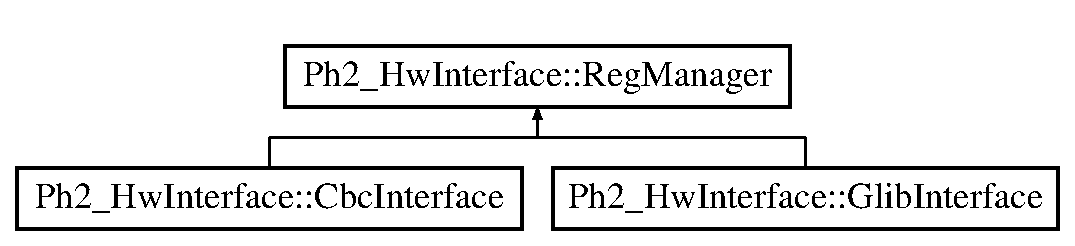
\includegraphics[height=2.000000cm]{class_ph2___hw_interface_1_1_reg_manager}
\end{center}
\end{figure}
\subsection*{Public Member Functions}
\begin{DoxyCompactItemize}
\item 
\hyperlink{class_ph2___hw_interface_1_1_reg_manager_a938f6b582b1fffcb478f35fd9d81954f}{Reg\-Manager} (const char $\ast$pu\-Hal\-Config\-File\-Name)
\begin{DoxyCompactList}\small\item\em Constructor of the \hyperlink{class_ph2___hw_interface_1_1_reg_manager}{Reg\-Manager} class. \end{DoxyCompactList}\item 
virtual \hyperlink{class_ph2___hw_interface_1_1_reg_manager_a5d650c4e6467153f98f999abbbfc354c}{$\sim$\-Reg\-Manager} ()
\begin{DoxyCompactList}\small\item\em Destructor of the \hyperlink{class_ph2___hw_interface_1_1_reg_manager}{Reg\-Manager} class. \end{DoxyCompactList}\item 
virtual void \hyperlink{class_ph2___hw_interface_1_1_reg_manager_a409c95948e25ea5fb7f897926e9de1e6}{Stack\-Reg} (const std\-::string \&p\-Reg\-Node, const uint32\-\_\-t \&p\-Val, bool p\-Send=false)
\end{DoxyCompactItemize}
\subsection*{Protected Member Functions}
\begin{DoxyCompactItemize}
\item 
virtual bool \hyperlink{class_ph2___hw_interface_1_1_reg_manager_a31174516fef6706c88c3f59dd93e4fdf}{Write\-Reg} (const std\-::string \&p\-Reg\-Node, const uint32\-\_\-t \&p\-Val)
\begin{DoxyCompactList}\small\item\em Write a register. \end{DoxyCompactList}\item 
virtual bool \hyperlink{class_ph2___hw_interface_1_1_reg_manager_ac67c49c17b1c171ef9836ae463d8bc18}{Write\-Stack\-Reg} (std\-::vector$<$ std\-::pair$<$ std\-::string, uint32\-\_\-t $>$ $>$ \&p\-Vec\-Reg)
\begin{DoxyCompactList}\small\item\em Write a stack of registers. \end{DoxyCompactList}\item 
virtual bool \hyperlink{class_ph2___hw_interface_1_1_reg_manager_a888f5cccb05daa28896cf622abfdcbd6}{Write\-Block\-Reg} (const std\-::string \&p\-Reg\-Node, const std\-::vector$<$ uint32\-\_\-t $>$ \&p\-Values)
\begin{DoxyCompactList}\small\item\em Write a block of values in a register. \end{DoxyCompactList}\item 
virtual uhal\-::\-Val\-Word$<$ uint32\-\_\-t $>$ \hyperlink{class_ph2___hw_interface_1_1_reg_manager_a077e0a18592206365150680213345112}{Read\-Reg} (const std\-::string \&p\-Reg\-Node)
\begin{DoxyCompactList}\small\item\em Read a value in a register. \end{DoxyCompactList}\item 
virtual uhal\-::\-Val\-Vector$<$ uint32\-\_\-t $>$ \hyperlink{class_ph2___hw_interface_1_1_reg_manager_a6481c211d27badc409ff0e7af20575e4}{Read\-Block\-Reg} (const std\-::string \&p\-Reg\-Node, const uint32\-\_\-t \&p\-Blocksize)
\begin{DoxyCompactList}\small\item\em Read a block of values in a register. \end{DoxyCompactList}\item 
virtual void \hyperlink{class_ph2___hw_interface_1_1_reg_manager_ab4e24cf318772c09a6c7e24b88b1dedb}{Stack\-Write\-Time\-Out} ()
\begin{DoxyCompactList}\small\item\em Stack the commands, deliver when full or timeout. \end{DoxyCompactList}\item 
virtual void \hyperlink{class_ph2___hw_interface_1_1_reg_manager_a20c502bcad5115c6ae16d4d356b72f0c}{Choose\-Board} (uint8\-\_\-t p\-Board\-Id)
\begin{DoxyCompactList}\small\item\em Choose the board we want to talk with. \end{DoxyCompactList}\end{DoxyCompactItemize}
\subsection*{Protected Attributes}
\begin{DoxyCompactItemize}
\item 
uhal\-::\-Hw\-Interface $\ast$ \hyperlink{class_ph2___hw_interface_1_1_reg_manager_a0d4908ec834a3a0b7d8139872fd0a4a0}{f\-Board}
\item 
const char $\ast$ \hyperlink{class_ph2___hw_interface_1_1_reg_manager_aaaa29ca65c283acc645132c7bef0f24f}{f\-U\-Hal\-Config\-File\-Name}
\item 
std\-::map$<$ uint8\-\_\-t, \\*
uhal\-::\-Hw\-Interface $\ast$ $>$ \hyperlink{class_ph2___hw_interface_1_1_reg_manager_a9c34ffe467a572796c05036533bb6d39}{f\-Board\-Map}
\item 
std\-::vector$<$ std\-::pair\\*
$<$ std\-::string, uint32\-\_\-t $>$ $>$ \hyperlink{class_ph2___hw_interface_1_1_reg_manager_a382c1c2373fde66d98a44e4aa0208e81}{f\-Stack\-Reg}
\item 
std\-::thread \hyperlink{class_ph2___hw_interface_1_1_reg_manager_a3aa2f1c4769f122a2e902f2d70865b30}{f\-Thread}
\item 
bool \hyperlink{class_ph2___hw_interface_1_1_reg_manager_ae337041a55b10db74bbd8e171424807a}{f\-Deactive\-Thread}
\item 
std\-::mutex \hyperlink{class_ph2___hw_interface_1_1_reg_manager_ab5fdbe722820897d3a1344f300cc4a92}{f\-Board\-Mutex}
\end{DoxyCompactItemize}


\subsection{Detailed Description}
Permit connection to given boards and r/w given registers. 

\subsection{Constructor \& Destructor Documentation}
\hypertarget{class_ph2___hw_interface_1_1_reg_manager_a938f6b582b1fffcb478f35fd9d81954f}{\index{Ph2\-\_\-\-Hw\-Interface\-::\-Reg\-Manager@{Ph2\-\_\-\-Hw\-Interface\-::\-Reg\-Manager}!Reg\-Manager@{Reg\-Manager}}
\index{Reg\-Manager@{Reg\-Manager}!Ph2_HwInterface::RegManager@{Ph2\-\_\-\-Hw\-Interface\-::\-Reg\-Manager}}
\subsubsection[{Reg\-Manager}]{\setlength{\rightskip}{0pt plus 5cm}Ph2\-\_\-\-Hw\-Interface\-::\-Reg\-Manager\-::\-Reg\-Manager (
\begin{DoxyParamCaption}
\item[{const char $\ast$}]{pu\-Hal\-Config\-File\-Name}
\end{DoxyParamCaption}
)}}\label{class_ph2___hw_interface_1_1_reg_manager_a938f6b582b1fffcb478f35fd9d81954f}


Constructor of the \hyperlink{class_ph2___hw_interface_1_1_reg_manager}{Reg\-Manager} class. 


\begin{DoxyParams}{Parameters}
{\em pu\-Hal\-Config\-File\-Name} & \-: path of the u\-Hal Config File \\
\hline
\end{DoxyParams}
\hypertarget{class_ph2___hw_interface_1_1_reg_manager_a5d650c4e6467153f98f999abbbfc354c}{\index{Ph2\-\_\-\-Hw\-Interface\-::\-Reg\-Manager@{Ph2\-\_\-\-Hw\-Interface\-::\-Reg\-Manager}!$\sim$\-Reg\-Manager@{$\sim$\-Reg\-Manager}}
\index{$\sim$\-Reg\-Manager@{$\sim$\-Reg\-Manager}!Ph2_HwInterface::RegManager@{Ph2\-\_\-\-Hw\-Interface\-::\-Reg\-Manager}}
\subsubsection[{$\sim$\-Reg\-Manager}]{\setlength{\rightskip}{0pt plus 5cm}Ph2\-\_\-\-Hw\-Interface\-::\-Reg\-Manager\-::$\sim$\-Reg\-Manager (
\begin{DoxyParamCaption}
{}
\end{DoxyParamCaption}
)\hspace{0.3cm}{\ttfamily [virtual]}}}\label{class_ph2___hw_interface_1_1_reg_manager_a5d650c4e6467153f98f999abbbfc354c}


Destructor of the \hyperlink{class_ph2___hw_interface_1_1_reg_manager}{Reg\-Manager} class. 



\subsection{Member Function Documentation}
\hypertarget{class_ph2___hw_interface_1_1_reg_manager_a20c502bcad5115c6ae16d4d356b72f0c}{\index{Ph2\-\_\-\-Hw\-Interface\-::\-Reg\-Manager@{Ph2\-\_\-\-Hw\-Interface\-::\-Reg\-Manager}!Choose\-Board@{Choose\-Board}}
\index{Choose\-Board@{Choose\-Board}!Ph2_HwInterface::RegManager@{Ph2\-\_\-\-Hw\-Interface\-::\-Reg\-Manager}}
\subsubsection[{Choose\-Board}]{\setlength{\rightskip}{0pt plus 5cm}void Ph2\-\_\-\-Hw\-Interface\-::\-Reg\-Manager\-::\-Choose\-Board (
\begin{DoxyParamCaption}
\item[{uint8\-\_\-t}]{p\-Board\-Id}
\end{DoxyParamCaption}
)\hspace{0.3cm}{\ttfamily [protected]}, {\ttfamily [virtual]}}}\label{class_ph2___hw_interface_1_1_reg_manager_a20c502bcad5115c6ae16d4d356b72f0c}


Choose the board we want to talk with. 


\begin{DoxyParams}{Parameters}
{\em p\-Board\-Id} & \-: Id of the Board to connect to \\
\hline
\end{DoxyParams}
\hypertarget{class_ph2___hw_interface_1_1_reg_manager_a6481c211d27badc409ff0e7af20575e4}{\index{Ph2\-\_\-\-Hw\-Interface\-::\-Reg\-Manager@{Ph2\-\_\-\-Hw\-Interface\-::\-Reg\-Manager}!Read\-Block\-Reg@{Read\-Block\-Reg}}
\index{Read\-Block\-Reg@{Read\-Block\-Reg}!Ph2_HwInterface::RegManager@{Ph2\-\_\-\-Hw\-Interface\-::\-Reg\-Manager}}
\subsubsection[{Read\-Block\-Reg}]{\setlength{\rightskip}{0pt plus 5cm}uhal\-::\-Val\-Vector$<$ uint32\-\_\-t $>$ Ph2\-\_\-\-Hw\-Interface\-::\-Reg\-Manager\-::\-Read\-Block\-Reg (
\begin{DoxyParamCaption}
\item[{const std\-::string \&}]{p\-Reg\-Node, }
\item[{const uint32\-\_\-t \&}]{p\-Blocksize}
\end{DoxyParamCaption}
)\hspace{0.3cm}{\ttfamily [protected]}, {\ttfamily [virtual]}}}\label{class_ph2___hw_interface_1_1_reg_manager_a6481c211d27badc409ff0e7af20575e4}


Read a block of values in a register. 


\begin{DoxyParams}{Parameters}
{\em p\-Reg\-Node} & \-: Node of the register to read \\
\hline
{\em p\-Blocksize} & \-: Size of the block to read \\
\hline
\end{DoxyParams}
\begin{DoxyReturn}{Returns}
Val\-Vector block values of the register 
\end{DoxyReturn}
\hypertarget{class_ph2___hw_interface_1_1_reg_manager_a077e0a18592206365150680213345112}{\index{Ph2\-\_\-\-Hw\-Interface\-::\-Reg\-Manager@{Ph2\-\_\-\-Hw\-Interface\-::\-Reg\-Manager}!Read\-Reg@{Read\-Reg}}
\index{Read\-Reg@{Read\-Reg}!Ph2_HwInterface::RegManager@{Ph2\-\_\-\-Hw\-Interface\-::\-Reg\-Manager}}
\subsubsection[{Read\-Reg}]{\setlength{\rightskip}{0pt plus 5cm}uhal\-::\-Val\-Word$<$ uint32\-\_\-t $>$ Ph2\-\_\-\-Hw\-Interface\-::\-Reg\-Manager\-::\-Read\-Reg (
\begin{DoxyParamCaption}
\item[{const std\-::string \&}]{p\-Reg\-Node}
\end{DoxyParamCaption}
)\hspace{0.3cm}{\ttfamily [protected]}, {\ttfamily [virtual]}}}\label{class_ph2___hw_interface_1_1_reg_manager_a077e0a18592206365150680213345112}


Read a value in a register. 


\begin{DoxyParams}{Parameters}
{\em p\-Reg\-Node} & \-: Node of the register to read \\
\hline
\end{DoxyParams}
\begin{DoxyReturn}{Returns}
Val\-Word value of the register 
\end{DoxyReturn}
\hypertarget{class_ph2___hw_interface_1_1_reg_manager_a409c95948e25ea5fb7f897926e9de1e6}{\index{Ph2\-\_\-\-Hw\-Interface\-::\-Reg\-Manager@{Ph2\-\_\-\-Hw\-Interface\-::\-Reg\-Manager}!Stack\-Reg@{Stack\-Reg}}
\index{Stack\-Reg@{Stack\-Reg}!Ph2_HwInterface::RegManager@{Ph2\-\_\-\-Hw\-Interface\-::\-Reg\-Manager}}
\subsubsection[{Stack\-Reg}]{\setlength{\rightskip}{0pt plus 5cm}void Ph2\-\_\-\-Hw\-Interface\-::\-Reg\-Manager\-::\-Stack\-Reg (
\begin{DoxyParamCaption}
\item[{const std\-::string \&}]{p\-Reg\-Node, }
\item[{const uint32\-\_\-t \&}]{p\-Val, }
\item[{bool}]{p\-Send = {\ttfamily false}}
\end{DoxyParamCaption}
)\hspace{0.3cm}{\ttfamily [virtual]}}}\label{class_ph2___hw_interface_1_1_reg_manager_a409c95948e25ea5fb7f897926e9de1e6}
\hypertarget{class_ph2___hw_interface_1_1_reg_manager_ab4e24cf318772c09a6c7e24b88b1dedb}{\index{Ph2\-\_\-\-Hw\-Interface\-::\-Reg\-Manager@{Ph2\-\_\-\-Hw\-Interface\-::\-Reg\-Manager}!Stack\-Write\-Time\-Out@{Stack\-Write\-Time\-Out}}
\index{Stack\-Write\-Time\-Out@{Stack\-Write\-Time\-Out}!Ph2_HwInterface::RegManager@{Ph2\-\_\-\-Hw\-Interface\-::\-Reg\-Manager}}
\subsubsection[{Stack\-Write\-Time\-Out}]{\setlength{\rightskip}{0pt plus 5cm}void Ph2\-\_\-\-Hw\-Interface\-::\-Reg\-Manager\-::\-Stack\-Write\-Time\-Out (
\begin{DoxyParamCaption}
{}
\end{DoxyParamCaption}
)\hspace{0.3cm}{\ttfamily [protected]}, {\ttfamily [virtual]}}}\label{class_ph2___hw_interface_1_1_reg_manager_ab4e24cf318772c09a6c7e24b88b1dedb}


Stack the commands, deliver when full or timeout. 


\begin{DoxyParams}{Parameters}
{\em Time} & Out for sending the register/value stack in the writting. It has only to be set in a detached thread from the one you're working on \\
\hline
\end{DoxyParams}
\hypertarget{class_ph2___hw_interface_1_1_reg_manager_a888f5cccb05daa28896cf622abfdcbd6}{\index{Ph2\-\_\-\-Hw\-Interface\-::\-Reg\-Manager@{Ph2\-\_\-\-Hw\-Interface\-::\-Reg\-Manager}!Write\-Block\-Reg@{Write\-Block\-Reg}}
\index{Write\-Block\-Reg@{Write\-Block\-Reg}!Ph2_HwInterface::RegManager@{Ph2\-\_\-\-Hw\-Interface\-::\-Reg\-Manager}}
\subsubsection[{Write\-Block\-Reg}]{\setlength{\rightskip}{0pt plus 5cm}bool Ph2\-\_\-\-Hw\-Interface\-::\-Reg\-Manager\-::\-Write\-Block\-Reg (
\begin{DoxyParamCaption}
\item[{const std\-::string \&}]{p\-Reg\-Node, }
\item[{const std\-::vector$<$ uint32\-\_\-t $>$ \&}]{p\-Values}
\end{DoxyParamCaption}
)\hspace{0.3cm}{\ttfamily [protected]}, {\ttfamily [virtual]}}}\label{class_ph2___hw_interface_1_1_reg_manager_a888f5cccb05daa28896cf622abfdcbd6}


Write a block of values in a register. 


\begin{DoxyParams}{Parameters}
{\em p\-Reg\-Node} & \-: Node of the register to write \\
\hline
{\em p\-Values} & \-: Block of values to write \\
\hline
\end{DoxyParams}
\begin{DoxyReturn}{Returns}
boolean confirming the writing 
\end{DoxyReturn}
\hypertarget{class_ph2___hw_interface_1_1_reg_manager_a31174516fef6706c88c3f59dd93e4fdf}{\index{Ph2\-\_\-\-Hw\-Interface\-::\-Reg\-Manager@{Ph2\-\_\-\-Hw\-Interface\-::\-Reg\-Manager}!Write\-Reg@{Write\-Reg}}
\index{Write\-Reg@{Write\-Reg}!Ph2_HwInterface::RegManager@{Ph2\-\_\-\-Hw\-Interface\-::\-Reg\-Manager}}
\subsubsection[{Write\-Reg}]{\setlength{\rightskip}{0pt plus 5cm}bool Ph2\-\_\-\-Hw\-Interface\-::\-Reg\-Manager\-::\-Write\-Reg (
\begin{DoxyParamCaption}
\item[{const std\-::string \&}]{p\-Reg\-Node, }
\item[{const uint32\-\_\-t \&}]{p\-Val}
\end{DoxyParamCaption}
)\hspace{0.3cm}{\ttfamily [protected]}, {\ttfamily [virtual]}}}\label{class_ph2___hw_interface_1_1_reg_manager_a31174516fef6706c88c3f59dd93e4fdf}


Write a register. 


\begin{DoxyParams}{Parameters}
{\em p\-Reg\-Node} & \-: Node of the register to write \\
\hline
{\em p\-Val} & \-: Value to write \\
\hline
\end{DoxyParams}
\begin{DoxyReturn}{Returns}
boolean confirming the writing 
\end{DoxyReturn}
\hypertarget{class_ph2___hw_interface_1_1_reg_manager_ac67c49c17b1c171ef9836ae463d8bc18}{\index{Ph2\-\_\-\-Hw\-Interface\-::\-Reg\-Manager@{Ph2\-\_\-\-Hw\-Interface\-::\-Reg\-Manager}!Write\-Stack\-Reg@{Write\-Stack\-Reg}}
\index{Write\-Stack\-Reg@{Write\-Stack\-Reg}!Ph2_HwInterface::RegManager@{Ph2\-\_\-\-Hw\-Interface\-::\-Reg\-Manager}}
\subsubsection[{Write\-Stack\-Reg}]{\setlength{\rightskip}{0pt plus 5cm}bool Ph2\-\_\-\-Hw\-Interface\-::\-Reg\-Manager\-::\-Write\-Stack\-Reg (
\begin{DoxyParamCaption}
\item[{std\-::vector$<$ std\-::pair$<$ std\-::string, uint32\-\_\-t $>$ $>$ \&}]{p\-Vec\-Reg}
\end{DoxyParamCaption}
)\hspace{0.3cm}{\ttfamily [protected]}, {\ttfamily [virtual]}}}\label{class_ph2___hw_interface_1_1_reg_manager_ac67c49c17b1c171ef9836ae463d8bc18}


Write a stack of registers. 


\begin{DoxyParams}{Parameters}
{\em p\-Vec\-Reg} & \-: vector containing the registers and the associated values to write \\
\hline
\end{DoxyParams}
\begin{DoxyReturn}{Returns}
boolean confirming the writing 
\end{DoxyReturn}


\subsection{Field Documentation}
\hypertarget{class_ph2___hw_interface_1_1_reg_manager_a0d4908ec834a3a0b7d8139872fd0a4a0}{\index{Ph2\-\_\-\-Hw\-Interface\-::\-Reg\-Manager@{Ph2\-\_\-\-Hw\-Interface\-::\-Reg\-Manager}!f\-Board@{f\-Board}}
\index{f\-Board@{f\-Board}!Ph2_HwInterface::RegManager@{Ph2\-\_\-\-Hw\-Interface\-::\-Reg\-Manager}}
\subsubsection[{f\-Board}]{\setlength{\rightskip}{0pt plus 5cm}uhal\-::\-Hw\-Interface$\ast$ Ph2\-\_\-\-Hw\-Interface\-::\-Reg\-Manager\-::f\-Board\hspace{0.3cm}{\ttfamily [protected]}}}\label{class_ph2___hw_interface_1_1_reg_manager_a0d4908ec834a3a0b7d8139872fd0a4a0}
Board in use \hypertarget{class_ph2___hw_interface_1_1_reg_manager_a9c34ffe467a572796c05036533bb6d39}{\index{Ph2\-\_\-\-Hw\-Interface\-::\-Reg\-Manager@{Ph2\-\_\-\-Hw\-Interface\-::\-Reg\-Manager}!f\-Board\-Map@{f\-Board\-Map}}
\index{f\-Board\-Map@{f\-Board\-Map}!Ph2_HwInterface::RegManager@{Ph2\-\_\-\-Hw\-Interface\-::\-Reg\-Manager}}
\subsubsection[{f\-Board\-Map}]{\setlength{\rightskip}{0pt plus 5cm}std\-::map$<$uint8\-\_\-t,uhal\-::\-Hw\-Interface$\ast$$>$ Ph2\-\_\-\-Hw\-Interface\-::\-Reg\-Manager\-::f\-Board\-Map\hspace{0.3cm}{\ttfamily [protected]}}}\label{class_ph2___hw_interface_1_1_reg_manager_a9c34ffe467a572796c05036533bb6d39}
Board Map with all known boards \hypertarget{class_ph2___hw_interface_1_1_reg_manager_ab5fdbe722820897d3a1344f300cc4a92}{\index{Ph2\-\_\-\-Hw\-Interface\-::\-Reg\-Manager@{Ph2\-\_\-\-Hw\-Interface\-::\-Reg\-Manager}!f\-Board\-Mutex@{f\-Board\-Mutex}}
\index{f\-Board\-Mutex@{f\-Board\-Mutex}!Ph2_HwInterface::RegManager@{Ph2\-\_\-\-Hw\-Interface\-::\-Reg\-Manager}}
\subsubsection[{f\-Board\-Mutex}]{\setlength{\rightskip}{0pt plus 5cm}std\-::mutex Ph2\-\_\-\-Hw\-Interface\-::\-Reg\-Manager\-::f\-Board\-Mutex\hspace{0.3cm}{\ttfamily [protected]}}}\label{class_ph2___hw_interface_1_1_reg_manager_ab5fdbe722820897d3a1344f300cc4a92}
Mutex to avoid conflict btw threads on shared resources \hypertarget{class_ph2___hw_interface_1_1_reg_manager_ae337041a55b10db74bbd8e171424807a}{\index{Ph2\-\_\-\-Hw\-Interface\-::\-Reg\-Manager@{Ph2\-\_\-\-Hw\-Interface\-::\-Reg\-Manager}!f\-Deactive\-Thread@{f\-Deactive\-Thread}}
\index{f\-Deactive\-Thread@{f\-Deactive\-Thread}!Ph2_HwInterface::RegManager@{Ph2\-\_\-\-Hw\-Interface\-::\-Reg\-Manager}}
\subsubsection[{f\-Deactive\-Thread}]{\setlength{\rightskip}{0pt plus 5cm}bool Ph2\-\_\-\-Hw\-Interface\-::\-Reg\-Manager\-::f\-Deactive\-Thread\hspace{0.3cm}{\ttfamily [protected]}}}\label{class_ph2___hw_interface_1_1_reg_manager_ae337041a55b10db74bbd8e171424807a}
Bool to terminate the thread in the destructor \hypertarget{class_ph2___hw_interface_1_1_reg_manager_a382c1c2373fde66d98a44e4aa0208e81}{\index{Ph2\-\_\-\-Hw\-Interface\-::\-Reg\-Manager@{Ph2\-\_\-\-Hw\-Interface\-::\-Reg\-Manager}!f\-Stack\-Reg@{f\-Stack\-Reg}}
\index{f\-Stack\-Reg@{f\-Stack\-Reg}!Ph2_HwInterface::RegManager@{Ph2\-\_\-\-Hw\-Interface\-::\-Reg\-Manager}}
\subsubsection[{f\-Stack\-Reg}]{\setlength{\rightskip}{0pt plus 5cm}std\-::vector$<$ std\-::pair$<$std\-::string,uint32\-\_\-t$>$ $>$ Ph2\-\_\-\-Hw\-Interface\-::\-Reg\-Manager\-::f\-Stack\-Reg\hspace{0.3cm}{\ttfamily [protected]}}}\label{class_ph2___hw_interface_1_1_reg_manager_a382c1c2373fde66d98a44e4aa0208e81}
Stack of registers \hypertarget{class_ph2___hw_interface_1_1_reg_manager_a3aa2f1c4769f122a2e902f2d70865b30}{\index{Ph2\-\_\-\-Hw\-Interface\-::\-Reg\-Manager@{Ph2\-\_\-\-Hw\-Interface\-::\-Reg\-Manager}!f\-Thread@{f\-Thread}}
\index{f\-Thread@{f\-Thread}!Ph2_HwInterface::RegManager@{Ph2\-\_\-\-Hw\-Interface\-::\-Reg\-Manager}}
\subsubsection[{f\-Thread}]{\setlength{\rightskip}{0pt plus 5cm}std\-::thread Ph2\-\_\-\-Hw\-Interface\-::\-Reg\-Manager\-::f\-Thread\hspace{0.3cm}{\ttfamily [protected]}}}\label{class_ph2___hw_interface_1_1_reg_manager_a3aa2f1c4769f122a2e902f2d70865b30}
Thread for timeout stack writing \hypertarget{class_ph2___hw_interface_1_1_reg_manager_aaaa29ca65c283acc645132c7bef0f24f}{\index{Ph2\-\_\-\-Hw\-Interface\-::\-Reg\-Manager@{Ph2\-\_\-\-Hw\-Interface\-::\-Reg\-Manager}!f\-U\-Hal\-Config\-File\-Name@{f\-U\-Hal\-Config\-File\-Name}}
\index{f\-U\-Hal\-Config\-File\-Name@{f\-U\-Hal\-Config\-File\-Name}!Ph2_HwInterface::RegManager@{Ph2\-\_\-\-Hw\-Interface\-::\-Reg\-Manager}}
\subsubsection[{f\-U\-Hal\-Config\-File\-Name}]{\setlength{\rightskip}{0pt plus 5cm}const char$\ast$ Ph2\-\_\-\-Hw\-Interface\-::\-Reg\-Manager\-::f\-U\-Hal\-Config\-File\-Name\hspace{0.3cm}{\ttfamily [protected]}}}\label{class_ph2___hw_interface_1_1_reg_manager_aaaa29ca65c283acc645132c7bef0f24f}
path of the u\-Hal Config File 

The documentation for this class was generated from the following files\-:\begin{DoxyCompactItemize}
\item 
H\-W\-Interface/\hyperlink{_reg_manager_8h}{Reg\-Manager.\-h}\item 
H\-W\-Interface/\hyperlink{_reg_manager_8cc}{Reg\-Manager.\-cc}\end{DoxyCompactItemize}

\chapter{File Documentation}
\input{_be_board_8cc}
\hypertarget{_be_board_8h}{\section{H\-W\-Description/\-Be\-Board.h File Reference}
\label{_be_board_8h}\index{H\-W\-Description/\-Be\-Board.\-h@{H\-W\-Description/\-Be\-Board.\-h}}
}


Be\-Board Description class, configs of the Be\-Board.  


{\ttfamily \#include \char`\"{}Definition.\-h\char`\"{}}\\*
{\ttfamily \#include \char`\"{}Module.\-h\char`\"{}}\\*
{\ttfamily \#include $<$vector$>$}\\*
{\ttfamily \#include $<$map$>$}\\*
{\ttfamily \#include $<$boost/cstdint.\-hpp$>$}\\*
\subsection*{Data Structures}
\begin{DoxyCompactItemize}
\item 
class \hyperlink{class_ph2___hw_description_1_1_be_board}{Ph2\-\_\-\-Hw\-Description\-::\-Be\-Board}
\begin{DoxyCompactList}\small\item\em Read/\-Write \hyperlink{class_ph2___hw_description_1_1_be_board}{Be\-Board}'s registers on a file, contains a register map and contains a vector of \hyperlink{class_ph2___hw_description_1_1_module}{Module} which are connected to the \hyperlink{class_ph2___hw_description_1_1_be_board}{Be\-Board}. \end{DoxyCompactList}\end{DoxyCompactItemize}
\subsection*{Namespaces}
\begin{DoxyCompactItemize}
\item 
\hyperlink{namespace_ph2___hw_description}{Ph2\-\_\-\-Hw\-Description}
\begin{DoxyCompactList}\small\item\em Namespace regrouping all the hardware description. \end{DoxyCompactList}\end{DoxyCompactItemize}
\subsection*{Typedefs}
\begin{DoxyCompactItemize}
\item 
typedef std\-::map$<$ std\-::string, \\*
uint16\-\_\-t $>$ \hyperlink{namespace_ph2___hw_description_a2e13fb82c8ed98154c60f9d0f8467d72}{Ph2\-\_\-\-Hw\-Description\-::\-Be\-Board\-Reg\-Map}
\end{DoxyCompactItemize}
\subsection*{Enumerations}
\begin{DoxyCompactItemize}
\item 
enum \hyperlink{namespace_ph2___hw_description_a891c19542f306c932b747f42fe48fc2b}{Ph2\-\_\-\-Hw\-Description\-::nb\-\_\-\-F\-E} \{ \hyperlink{namespace_ph2___hw_description_a891c19542f306c932b747f42fe48fc2baa30d72f6d58dc25b003fbf8bf56b3ace}{Ph2\-\_\-\-Hw\-Description\-::\-S\-I\-N\-G\-L\-E\-\_\-\-F\-E}, 
\hyperlink{namespace_ph2___hw_description_a891c19542f306c932b747f42fe48fc2ba6e0b877d015d017f61b07618e057c452}{Ph2\-\_\-\-Hw\-Description\-::\-F\-E\-\_\-\-T\-R\-G}, 
\hyperlink{namespace_ph2___hw_description_a891c19542f306c932b747f42fe48fc2bae3b57cb16641bb367bfc57a00315a4ca}{Ph2\-\_\-\-Hw\-Description\-::\-D\-U\-A\-L\-\_\-\-F\-E}
 \}
\end{DoxyCompactItemize}


\subsection{Detailed Description}
Be\-Board Description class, configs of the Be\-Board. \begin{DoxyAuthor}{Author}
Lorenzo B\-I\-D\-E\-G\-A\-I\-N 
\end{DoxyAuthor}
\begin{DoxyDate}{Date}
14/07/14
\end{DoxyDate}
Support \-: mail to \-: \href{mailto:lorenzo.bidegain@cern.ch}{\tt lorenzo.\-bidegain@cern.\-ch} 
\input{_cbc_8cc}
\input{_cbc_8h}
\input{_cbc_reg_item_8h}
\hypertarget{_definition_8h}{\section{H\-W\-Description/\-Definition.h File Reference}
\label{_definition_8h}\index{H\-W\-Description/\-Definition.\-h@{H\-W\-Description/\-Definition.\-h}}
}
\subsection*{Macros}
\begin{DoxyCompactItemize}
\item 
\#define \hyperlink{_definition_8h_a887b6fc7c99e60908c9f185fff066443}{U\-H\-A\-L\-\_\-\-C\-O\-N\-N\-E\-C\-T\-I\-O\-N\-\_\-\-F\-I\-L\-E}~\char`\"{}file\-:///afs/cern.\-ch/user/n/npierre/2\-C\-B\-C/settings/connections.\-xml\char`\"{}
\item 
\#define \hyperlink{_definition_8h_a9a33e5f7e6ec12c2dd3f55317c6c16f1}{D\-E\-F\-A\-U\-L\-T\-\_\-\-G\-L\-I\-B\-\_\-\-F\-I\-L\-E}~\char`\"{}settings/glib\-\_\-settings.\-cfg\char`\"{}
\item 
\#define \hyperlink{_definition_8h_a5dc29b5a1e12da7983d60e10635114da}{D\-E\-F\-A\-U\-L\-T\-\_\-\-F\-I\-L\-E}~\char`\"{}settings/default\-\_\-file.\-txt\char`\"{}
\item 
\#define \hyperlink{_definition_8h_a3fae339a37a0fe73d984b3aab670d592}{F\-E0\-C\-B\-C0\-H\-O\-L\-E}~\char`\"{}settings/F\-E0\-C\-B\-C0\-Hole.\-txt\char`\"{}
\item 
\#define \hyperlink{_definition_8h_a94c8858f23020abc363336aeb9a5713c}{F\-E0\-C\-B\-C1}~\char`\"{}settings/F\-E0\-C\-B\-C1.\-txt\char`\"{}
\item 
\#define \hyperlink{_definition_8h_a5b3a756582189084a13c551862ca14c8}{F\-E0\-C\-B\-C1\-H\-O\-L\-E}~\char`\"{}settings/F\-E0\-C\-B\-C1\-Hole.\-txt\char`\"{}
\item 
\#define \hyperlink{_definition_8h_a7538d40fca6562ecc1768f6d07cef2fa}{I2\-C\-\_\-\-C\-T\-R\-L\-\_\-\-E\-N\-A\-B\-L\-E}~0x000009\-F4
\item 
\#define \hyperlink{_definition_8h_ab1dd2d69bec1712857cc2a103c85c26d}{I2\-C\-\_\-\-C\-T\-R\-L\-\_\-\-D\-I\-S\-A\-B\-L\-E}~0
\item 
\#define \hyperlink{_definition_8h_a8d3f448d28b023f560e3df976bb3ff9c}{I2\-C\-\_\-\-S\-T\-R\-O\-B\-E}~1
\item 
\#define \hyperlink{_definition_8h_aae239b4919cbd8d8dced934150986de3}{I2\-C\-\_\-\-M16\-B}~0
\item 
\#define \hyperlink{_definition_8h_ac030aa7b3fbd8b2432a9c66fc49fc4ae}{I2\-C\-\_\-\-M\-E\-M}~1
\item 
\#define \hyperlink{_definition_8h_a7978167075eb8954c1090fc7ce9647c6}{I2\-C\-\_\-\-W\-R\-I\-T\-E\-\_\-\-A\-D\-D\-R}~0x09
\item 
\#define \hyperlink{_definition_8h_a11a0148c64950f3315f38d957cd43d37}{I2\-C\-\_\-\-R\-E\-A\-D\-\_\-\-A\-D\-D\-R}~0x06
\item 
\#define \hyperlink{_definition_8h_ab15137f7c592d05573de99f078516157}{I2\-C\-\_\-\-S\-L\-A\-V\-E}~0x5\-B
\item 
\#define \hyperlink{_definition_8h_ae308275dafb538f2511ea285fea768d0}{I2\-C\-\_\-\-C\-O\-M\-M\-A\-N\-D}~\char`\"{}user\-\_\-wb\-\_\-ttc\-\_\-fmc\-\_\-regs.\-cbc\-\_\-reg\-\_\-i2c\-\_\-command\char`\"{}
\item 
\#define \hyperlink{_definition_8h_a46aaa2293185dfc3cd655f65bea7f614}{I2\-C\-\_\-\-R\-E\-P\-L\-Y}~\char`\"{}user\-\_\-wb\-\_\-ttc\-\_\-fmc\-\_\-regs.\-cbc\-\_\-reg\-\_\-i2c\-\_\-reply\char`\"{}
\item 
\#define \hyperlink{_definition_8h_a15db09e24617ea5c5843213672ac8a03}{I2\-C\-\_\-\-S\-E\-T\-T\-I\-N\-G\-S}~\char`\"{}user\-\_\-wb\-\_\-ttc\-\_\-fmc\-\_\-regs.\-cbc\-\_\-reg\-\_\-i2c\-\_\-settings\char`\"{}
\item 
\#define \hyperlink{_definition_8h_a30957298974d3b5c605a9e6e3cf33ff9}{M\-A\-X\-\_\-\-N\-B\-\_\-\-L\-O\-O\-P}~100
\item 
\#define \hyperlink{_definition_8h_a9b229c5fa667622ae84c26cbbfca2c4a}{B\-O\-A\-R\-D\-\_\-\-T\-Y\-P\-E}~\char`\"{}board\-\_\-id\char`\"{}
\item 
\#define \hyperlink{_definition_8h_a5a209f781c62e738bb2f3868604fbe77}{F\-W\-\_\-\-V\-E\-R\-S\-I\-O\-N\-\_\-\-M\-A\-J\-O\-R}~\char`\"{}firm\-\_\-id.\-firmware\-\_\-major\char`\"{}
\item 
\#define \hyperlink{_definition_8h_ae224d2fae5df95eef5b8b1638b714731}{F\-W\-\_\-\-V\-E\-R\-S\-I\-O\-N\-\_\-\-M\-I\-N\-O\-R}~\char`\"{}firm\-\_\-id.\-firmware\-\_\-minor\char`\"{}
\item 
\#define \hyperlink{_definition_8h_a46d23f1b70547c7ec03a7ede5a4a53c1}{F\-W\-\_\-\-V\-E\-R\-S\-I\-O\-N\-\_\-\-B\-U\-I\-L\-D}~\char`\"{}firm\-\_\-id.\-firmware\-\_\-build\char`\"{}
\item 
\#define \hyperlink{_definition_8h_ace8447cf1974d876d5655fb2fb48f7a9}{F\-M\-C1\-\_\-\-P\-R\-E\-S\-E\-N\-T}~\char`\"{}status.\-fmc1\-\_\-present\char`\"{}
\item 
\#define \hyperlink{_definition_8h_adc6f5f1944441c702829bb535878c480}{F\-M\-C2\-\_\-\-P\-R\-E\-S\-E\-N\-T}~\char`\"{}status.\-fmc2\-\_\-present\char`\"{}
\item 
\#define \hyperlink{_definition_8h_a6124cfaca7b122eb740cc81165fdb52d}{F\-M\-C\-\_\-\-U\-S\-E\-R\-\_\-\-B\-O\-A\-R\-D\-\_\-\-I\-D}~\char`\"{}user\-\_\-wb\-\_\-ttc\-\_\-fmc\-\_\-regs.\-user\-\_\-board\-\_\-id\char`\"{}
\item 
\#define \hyperlink{_definition_8h_a63344015089bba1295e33de70c0bd6d1}{F\-M\-C\-\_\-\-U\-S\-E\-R\-\_\-\-S\-Y\-S\-\_\-\-I\-D}~\char`\"{}user\-\_\-wb\-\_\-ttc\-\_\-fmc\-\_\-regs.\-user\-\_\-sys\-\_\-id\char`\"{}
\item 
\#define \hyperlink{_definition_8h_ae326374c67375e752225499c19882801}{F\-M\-C\-\_\-\-U\-S\-E\-R\-\_\-\-V\-E\-R\-S\-I\-O\-N}~\char`\"{}user\-\_\-wb\-\_\-ttc\-\_\-fmc\-\_\-regs.\-user\-\_\-version\char`\"{}
\item 
\#define \hyperlink{_definition_8h_a6a7f90395054dfa1a2f6521213aad848}{S\-R\-A\-M1}~\char`\"{}sram1\char`\"{}
\item 
\#define \hyperlink{_definition_8h_a14684bbbabb20ef143bc395b2c7e2ed9}{S\-R\-A\-M2}~\char`\"{}sram2\char`\"{}
\item 
\#define \hyperlink{_definition_8h_adf5585d61d19b17bc9af074a461fde93}{S\-R\-A\-M1\-\_\-\-U\-S\-R\-\_\-\-L\-O\-G\-I\-C}~\char`\"{}ctrl\-\_\-sram.\-sram1\-\_\-user\-\_\-logic\char`\"{}
\item 
\#define \hyperlink{_definition_8h_ad891becc0588c44642479f53d559c1a5}{S\-R\-A\-M2\-\_\-\-U\-S\-R\-\_\-\-L\-O\-G\-I\-C}~\char`\"{}ctrl\-\_\-sram.\-sram2\-\_\-user\-\_\-logic\char`\"{}
\item 
\#define \hyperlink{_definition_8h_a96bfb08d3abc89fde1c50f2db0b640de}{S\-R\-A\-M1\-\_\-\-E\-N\-D\-\_\-\-R\-E\-A\-D\-O\-U\-T}~\char`\"{}user\-\_\-wb\-\_\-ttc\-\_\-fmc\-\_\-regs.\-pc\-\_\-commands.\-S\-R\-A\-M1\-\_\-end\-\_\-readout\char`\"{}
\item 
\#define \hyperlink{_definition_8h_adf4e9d9d29b9c2e8e501dae3131be2a3}{S\-R\-A\-M2\-\_\-\-E\-N\-D\-\_\-\-R\-E\-A\-D\-O\-U\-T}~\char`\"{}user\-\_\-wb\-\_\-ttc\-\_\-fmc\-\_\-regs.\-pc\-\_\-commands.\-S\-R\-A\-M2\-\_\-end\-\_\-readout\char`\"{}
\item 
\#define \hyperlink{_definition_8h_a08761f200e1c7a6fe97e09d7af9c7a15}{S\-R\-A\-M1\-\_\-\-F\-U\-L\-L}~\char`\"{}user\-\_\-wb\-\_\-ttc\-\_\-fmc\-\_\-regs.\-flags.\-S\-R\-A\-M1\-\_\-full\char`\"{}
\item 
\#define \hyperlink{_definition_8h_a937e26b9dc4d1f265bbc8982b410451b}{S\-R\-A\-M2\-\_\-\-F\-U\-L\-L}~\char`\"{}user\-\_\-wb\-\_\-ttc\-\_\-fmc\-\_\-regs.\-flags.\-S\-R\-A\-M2\-\_\-full\char`\"{}
\item 
\#define \hyperlink{_definition_8h_a6190016044b4e4aafb00bc3767600a34}{F\-A\-K\-E\-\_\-\-D\-A\-T\-A}~\char`\"{}user\-\_\-wb\-\_\-ttc\-\_\-fmc\-\_\-regs.\-pc\-\_\-commands.\-C\-B\-C\-\_\-\-D\-A\-T\-A\-\_\-\-G\-E\-N\-E\char`\"{}
\item 
\#define \hyperlink{_definition_8h_ac2006ced84fd829c1eaea6ee77c73fce}{E\-X\-T\-\_\-\-T\-R\-G}~\char`\"{}user\-\_\-wb\-\_\-ttc\-\_\-fmc\-\_\-regs.\-pc\-\_\-commands.\-T\-R\-I\-G\-G\-E\-R\-\_\-\-S\-E\-L\char`\"{}
\item 
\#define \hyperlink{_definition_8h_a67670806b37e9b321f2d1dc4a45f55a2}{H\-Y\-B\-R\-I\-D\-\_\-\-T\-Y\-P\-E}~\char`\"{}user\-\_\-wb\-\_\-ttc\-\_\-fmc\-\_\-regs.\-new.\-hybrid\-\_\-type\char`\"{}
\item 
\#define \hyperlink{_definition_8h_a7da27b2738428e3dfeb39e351e551556}{C\-B\-C\-\_\-\-E\-X\-P\-E\-C\-T\-E\-D}~\char`\"{}C\-B\-C\-\_\-expected\char`\"{}
\item 
\#define \hyperlink{_definition_8h_a4c95b734f201124f65fdf525484f905c}{C\-B\-C\-\_\-\-P\-A\-C\-K\-E\-T\-\_\-\-N\-B}~\char`\"{}user\-\_\-wb\-\_\-ttc\-\_\-fmc\-\_\-regs.\-pc\-\_\-commands.\-C\-B\-C\-\_\-\-D\-A\-T\-A\-\_\-\-P\-A\-C\-K\-E\-T\-\_\-\-N\-U\-M\-B\-E\-R\char`\"{}
\item 
\#define \hyperlink{_definition_8h_ab41e5a6624129af07cf04896a2638e05}{C\-B\-C\-\_\-\-T\-E\-S\-T\-\_\-\-P\-U\-L\-S\-E\-\_\-\-V\-A\-L\-I\-D}~\char`\"{}C\-O\-M\-M\-I\-S\-S\-I\-O\-N\-N\-I\-N\-G\-\_\-\-M\-O\-D\-E\-\_\-\-C\-B\-C\-\_\-\-T\-E\-S\-T\-\_\-\-P\-U\-L\-S\-E\-\_\-\-V\-A\-L\-I\-D\char`\"{}
\item 
\#define \hyperlink{_definition_8h_aa8b47c8d93bc3a0a17f13d7aba88eebd}{C\-B\-C\-\_\-\-D\-A\-T\-A\-\_\-\-G\-E\-N\-E}~\char`\"{}user\-\_\-wb\-\_\-ttc\-\_\-fmc\-\_\-regs.\-pc\-\_\-commands.\-C\-B\-C\-\_\-\-D\-A\-T\-A\-\_\-\-G\-E\-N\-E\char`\"{}
\item 
\#define \hyperlink{_definition_8h_af707b6c693823387a84c1ae5b5dc01c7}{C\-B\-C\-\_\-\-T\-R\-I\-G\-G\-E\-R\-\_\-1\-S\-H\-O\-T}~\char`\"{}user\-\_\-wb\-\_\-ttc\-\_\-fmc\-\_\-regs.\-cbc\-\_\-acquisition.\-C\-B\-C\-\_\-\-T\-R\-I\-G\-G\-E\-R\-\_\-\-O\-N\-E\-\_\-\-S\-H\-O\-T\char`\"{}
\item 
\#define \hyperlink{_definition_8h_a74f2bb936c6db739349d53796624df22}{C\-B\-C\-\_\-\-S\-T\-U\-B\-\_\-\-L\-A\-T\-E\-N\-C\-Y}~\char`\"{}cbc\-\_\-stubdata\-\_\-latency\-\_\-adjust\char`\"{}
\item 
\#define \hyperlink{_definition_8h_adcbbe8574bdf346be21ae23451c410ec}{C\-B\-C\-\_\-\-S\-T\-U\-B\-\_\-\-L\-A\-T\-E\-N\-C\-Y\-\_\-\-F\-E1}~\char`\"{}cbc\-\_\-stubdata\-\_\-latency\-\_\-adjust\-\_\-fe1\char`\"{}
\item 
\#define \hyperlink{_definition_8h_a99153490571202993a0d92d1ffb62df0}{C\-B\-C\-\_\-\-S\-T\-U\-B\-\_\-\-L\-A\-T\-E\-N\-C\-Y\-\_\-\-F\-E2}~\char`\"{}cbc\-\_\-stubdata\-\_\-latency\-\_\-adjust\-\_\-fe2\char`\"{}
\item 
\#define \hyperlink{_definition_8h_a980fdc4242ab14da9fcd648b1e9a50a4}{C\-B\-C\-\_\-\-I2\-C\-\_\-\-C\-M\-D\-\_\-\-A\-C\-K}~\char`\"{}cbc\-\_\-i2c\-\_\-cmd\-\_\-ack\char`\"{}
\item 
\#define \hyperlink{_definition_8h_a8a4f3b344351ac3f9e05f3a3d27ffbf6}{C\-B\-C\-\_\-\-I2\-C\-\_\-\-C\-M\-D\-\_\-\-A\-C\-K\-\_\-\-F\-E1}~\char`\"{}cbc\-\_\-i2c\-\_\-cmd\-\_\-ack\-\_\-fe1\char`\"{}
\item 
\#define \hyperlink{_definition_8h_ad7ef355ab00621a8d2984b3a4d2b5336}{C\-B\-C\-\_\-\-I2\-C\-\_\-\-C\-M\-D\-\_\-\-A\-C\-K\-\_\-\-F\-E2}~\char`\"{}cbc\-\_\-i2c\-\_\-cmd\-\_\-ack\-\_\-fe2\char`\"{}
\item 
\#define \hyperlink{_definition_8h_aa92f4a416201bbe9742da9f72ba0bb46}{C\-B\-C\-\_\-\-I2\-C\-\_\-\-C\-M\-D\-\_\-\-R\-Q}~\char`\"{}cbc\-\_\-i2c\-\_\-cmd\-\_\-rq\char`\"{}
\item 
\#define \hyperlink{_definition_8h_a27f1d47d65b52569c75ae7abb12c850c}{C\-B\-C\-\_\-\-I2\-C\-\_\-\-C\-M\-D\-\_\-\-R\-Q\-\_\-\-F\-E1}~\char`\"{}cbc\-\_\-i2c\-\_\-cmd\-\_\-rq\-\_\-fe1\char`\"{}
\item 
\#define \hyperlink{_definition_8h_a386e61ed089e53095e19b1dded969001}{C\-B\-C\-\_\-\-I2\-C\-\_\-\-C\-M\-D\-\_\-\-R\-Q\-\_\-\-F\-E2}~\char`\"{}cbc\-\_\-i2c\-\_\-cmd\-\_\-rq\-\_\-fe2\char`\"{}
\item 
\#define \hyperlink{_definition_8h_a339750768b74eeb2a5e15d27002e5ed1}{C\-B\-C\-\_\-\-H\-A\-R\-D\-\_\-\-R\-E\-S\-E\-T}~\char`\"{}cbc\-\_\-hard\-\_\-reset\char`\"{}
\item 
\#define \hyperlink{_definition_8h_a1afae7c30406c0520e384fa1806e97ca}{C\-B\-C\-\_\-\-H\-A\-R\-D\-\_\-\-R\-E\-S\-E\-T\-\_\-\-F\-E1}~\char`\"{}cbc\-\_\-hard\-\_\-reset\-\_\-fe1\char`\"{}
\item 
\#define \hyperlink{_definition_8h_ae6dcd5d0b1ff293b4ad62fe648e34127}{C\-B\-C\-\_\-\-H\-A\-R\-D\-\_\-\-R\-E\-S\-E\-T\-\_\-\-F\-E2}~\char`\"{}cbc\-\_\-hard\-\_\-reset\-\_\-fe2\char`\"{}
\item 
\#define \hyperlink{_definition_8h_a46c24affadd18b38f8f180c29996c917}{C\-B\-C\-\_\-\-F\-A\-S\-T\-\_\-\-R\-E\-S\-E\-T}~\char`\"{}cbc\-\_\-fast\-\_\-reset\char`\"{}
\item 
\#define \hyperlink{_definition_8h_a14ca43ce56b6ba3282562ec26d4dd1d4}{C\-B\-C\-\_\-\-F\-A\-S\-T\-\_\-\-R\-E\-S\-E\-T\-\_\-\-F\-E1}~\char`\"{}cbc\-\_\-fast\-\_\-reset\-\_\-fe1\char`\"{}
\item 
\#define \hyperlink{_definition_8h_aac0c28e4301536787f75b2b7c8f8a4ab}{C\-B\-C\-\_\-\-F\-A\-S\-T\-\_\-\-R\-E\-S\-E\-T\-\_\-\-F\-E2}~\char`\"{}cbc\-\_\-fast\-\_\-reset\-\_\-fe2\char`\"{}
\item 
\#define \hyperlink{_definition_8h_aa8f2e0c6d69fa30c6f3df3a1ce79191b}{D\-E\-L\-A\-Y\-\_\-\-A\-F\-\_\-\-F\-A\-S\-T\-\_\-\-R\-E\-S\-E\-T}~\char`\"{}C\-O\-M\-M\-I\-S\-S\-I\-O\-N\-N\-I\-N\-G\-\_\-\-M\-O\-D\-E\-\_\-\-D\-E\-L\-A\-Y\-\_\-\-A\-F\-T\-E\-R\-\_\-\-F\-A\-S\-T\-\_\-\-R\-E\-S\-E\-T\char`\"{}
\item 
\#define \hyperlink{_definition_8h_a54b90cd00f1ecb699b4addd24a1991f5}{D\-E\-L\-A\-Y\-\_\-\-A\-F\-\_\-\-L1\-A}~\char`\"{}C\-O\-M\-M\-I\-S\-S\-I\-O\-N\-N\-I\-N\-G\-\_\-\-M\-O\-D\-E\-\_\-\-D\-E\-L\-A\-Y\-\_\-\-A\-F\-T\-E\-R\-\_\-\-L1\-A\char`\"{}
\item 
\#define \hyperlink{_definition_8h_ade36f0b97b019d8e26695fc406262b42}{D\-E\-L\-A\-Y\-\_\-\-A\-F\-\_\-\-T\-E\-S\-T\-\_\-\-P\-U\-L\-S\-E}~\char`\"{}C\-O\-M\-M\-I\-S\-S\-I\-O\-N\-N\-I\-N\-G\-\_\-\-M\-O\-D\-E\-\_\-\-D\-E\-L\-A\-Y\-\_\-\-A\-F\-T\-E\-R\-\_\-\-T\-E\-S\-T\-\_\-\-P\-U\-L\-S\-E\char`\"{}
\item 
\#define \hyperlink{_definition_8h_a001a688d4bf711101d3b626ba6ae8726}{B\-R\-E\-A\-K\-\_\-\-T\-R\-I\-G\-G\-E\-R}~\char`\"{}break\-\_\-trigger\char`\"{}
\item 
\#define \hyperlink{_definition_8h_a11ea004b3c38d4dae3309a13db5b6f78}{I\-N\-T\-\_\-\-T\-R\-I\-G\-G\-E\-R\-\_\-\-F\-R\-E\-Q}~\char`\"{}user\-\_\-wb\-\_\-ttc\-\_\-fmc\-\_\-regs.\-pc\-\_\-commands.\-I\-N\-T\-\_\-\-T\-R\-I\-G\-G\-E\-R\-\_\-\-F\-R\-E\-Q\char`\"{}
\item 
\#define \hyperlink{_definition_8h_a1f0933a2debf91dff9cf62493a7d0225}{T\-R\-I\-G\-G\-E\-R\-\_\-\-S\-E\-L\-E\-C\-T}~\char`\"{}user\-\_\-wb\-\_\-ttc\-\_\-fmc\-\_\-regs.\-pc\-\_\-commands.\-T\-R\-I\-G\-G\-E\-R\-\_\-\-S\-E\-L\char`\"{}
\item 
\#define \hyperlink{_definition_8h_aaa08b81a680d7b782f1709b09969346b}{E\-V\-E\-N\-T\-\_\-\-N\-U\-M\-B\-E\-R}~100
\item 
\#define \hyperlink{_definition_8h_a99f68b90851a6e4f890bd520f4ae5a8f}{E\-V\-E\-N\-T\-\_\-\-S\-I\-Z\-E\-\_\-32}~4$\ast$9+6
\item 
\#define \hyperlink{_definition_8h_af02f6ff9a143548736b70c9b5dd340ef}{O\-F\-F\-S\-E\-T\-\_\-\-B\-U\-N\-C\-H}~8
\item 
\#define \hyperlink{_definition_8h_a80ed4da02244b01e9002b83b08622833}{W\-I\-D\-T\-H\-\_\-\-B\-U\-N\-C\-H}~24
\item 
\#define \hyperlink{_definition_8h_a7e3f5dcd64e350b19cfe6ac8d8b9de55}{O\-F\-F\-S\-E\-T\-\_\-\-O\-R\-B\-I\-T}~1$\ast$32+8
\item 
\#define \hyperlink{_definition_8h_aa9aa442bb5c1632ae55291cc8745df4f}{W\-I\-D\-T\-H\-\_\-\-O\-R\-B\-I\-T}~24
\item 
\#define \hyperlink{_definition_8h_aa726e7f33789f31d51f8e23c8027331f}{O\-F\-F\-S\-E\-T\-\_\-\-L\-U\-M\-I}~2$\ast$32+8
\item 
\#define \hyperlink{_definition_8h_a8e0d7d1baf50ff405315799885e5fe1f}{W\-I\-D\-T\-H\-\_\-\-L\-U\-M\-I}~24
\item 
\#define \hyperlink{_definition_8h_a19dec49d149ed0fe8b2b40b897e02a0a}{O\-F\-F\-S\-E\-T\-\_\-\-E\-V\-E\-N\-T\-\_\-\-C\-O\-U\-N\-T}~3$\ast$32+8
\item 
\#define \hyperlink{_definition_8h_a7ffea0c86604775c2c6f3eb39b721439}{W\-I\-D\-T\-H\-\_\-\-E\-V\-E\-N\-T\-\_\-\-C\-O\-U\-N\-T}~24
\item 
\#define \hyperlink{_definition_8h_aebd462ec6df98e8ed895658b76d46b0a}{O\-F\-F\-S\-E\-T\-\_\-\-E\-V\-E\-N\-T\-\_\-\-C\-O\-U\-N\-T\-\_\-\-C\-B\-C}~4$\ast$32+8
\item 
\#define \hyperlink{_definition_8h_a8a9f30d30ccc6d269a97f1a7fd278a0a}{W\-I\-D\-T\-H\-\_\-\-E\-V\-E\-N\-T\-\_\-\-C\-O\-U\-N\-T\-\_\-\-C\-B\-C}~3$\ast$8
\item 
\#define \hyperlink{_definition_8h_a169ef5cf3d45b89a73525ce7856a9c10}{O\-F\-F\-S\-E\-T\-\_\-\-F\-E\-\_\-\-E\-V\-E\-N\-T}~5$\ast$4
\item 
\#define \hyperlink{_definition_8h_a472dc6061c390a709875f8aff275b224}{W\-I\-D\-T\-H\-\_\-\-F\-E\-\_\-\-E\-V\-E\-N\-T}~9$\ast$4$\ast$2
\item 
\#define \hyperlink{_definition_8h_ab92be247eb48959138e31f51abdb4595}{O\-F\-F\-S\-E\-T\-\_\-\-T\-D\-C}~5$\ast$32+9$\ast$4$\ast$2
\item 
\#define \hyperlink{_definition_8h_a35a886560b7c229138c6d0cf9d49bb8d}{W\-I\-D\-T\-H\-\_\-\-T\-D\-C}~32
\item 
\#define \hyperlink{_definition_8h_a48e38123a19c8946d3f3d43e397aac44}{F\-E\-\_\-\-N\-C\-H\-A\-R}~9$\ast$4$\ast$2
\item 
\#define \hyperlink{_definition_8h_aaa87103510bece40808b6bd48b0816de}{N\-S\-E\-N\-S\-O\-R}~254
\item 
\#define \hyperlink{_definition_8h_ad2bc6c3edfeacef111e6c48a1e7d4292}{O\-F\-F\-S\-E\-T\-\_\-\-E\-R\-R\-O\-R}~0
\item 
\#define \hyperlink{_definition_8h_a2631e8313c2ad88efde5a688e59268b1}{W\-I\-D\-T\-H\-\_\-\-E\-R\-R\-O\-R}~2
\item 
\#define \hyperlink{_definition_8h_a5868314549e40a5df9050c0aefdd28d5}{O\-F\-F\-S\-E\-T\-\_\-\-P\-I\-P\-E\-L\-I\-N\-E\-\_\-\-A\-D\-D\-R\-E\-S\-S}~2
\item 
\#define \hyperlink{_definition_8h_a700bfc7826a1bf6c5a0d70b702c686a1}{W\-I\-D\-T\-H\-\_\-\-P\-I\-P\-E\-L\-I\-N\-E\-\_\-\-A\-D\-D\-R\-E\-S\-S}~8
\item 
\#define \hyperlink{_definition_8h_a1314086b8661fda4ef495c9bb7acc09c}{O\-F\-F\-S\-E\-T\-\_\-\-C\-B\-C\-D\-A\-T\-A}~2+8
\item 
\#define \hyperlink{_definition_8h_a0769a751209824a05e5036e98a1f8ffd}{W\-I\-D\-T\-H\-\_\-\-C\-B\-C\-D\-A\-T\-A}~254
\item 
\#define \hyperlink{_definition_8h_a5bc72cc73fd4c639404f07920d4e4a32}{O\-F\-F\-S\-E\-T\-\_\-\-G\-L\-I\-B\-F\-L\-A\-G}~10+254
\item 
\#define \hyperlink{_definition_8h_a1ce95bad2fed3f0ae933f08daa0961e6}{W\-I\-D\-T\-H\-\_\-\-G\-L\-I\-B\-F\-L\-A\-G}~12
\item 
\#define \hyperlink{_definition_8h_aa9d274ac8baab1202ecfade41a222123}{O\-F\-F\-S\-E\-T\-\_\-\-C\-B\-C\-S\-T\-A\-B\-D\-A\-T\-A}~264+12
\item 
\#define \hyperlink{_definition_8h_a2ae263eeff9ce8a6b740a21726914ce8}{W\-I\-D\-T\-H\-\_\-\-C\-B\-C\-S\-T\-A\-B\-D\-A\-T\-A}~12
\item 
\#define \hyperlink{_definition_8h_ad6f5a85a8f621db82c92957e53000b61}{C\-B\-C\-\_\-\-N\-C\-H\-A\-R}~9$\ast$4
\item 
\#define \hyperlink{_definition_8h_a1489698bb660d3265c22ac35ab990bdc}{P\-C\-\_\-\-C\-O\-N\-F\-I\-G\-\_\-\-O\-K}~\char`\"{}user\-\_\-wb\-\_\-ttc\-\_\-fmc\-\_\-regs.\-pc\-\_\-commands.\-P\-C\-\_\-config\-\_\-ok\char`\"{}
\item 
\#define \hyperlink{_definition_8h_ab207427d943afb5b5fc19364720a69a7}{S\-P\-U\-R\-I\-O\-U\-S\-\_\-\-F\-R\-A\-M\-E}~\char`\"{}user\-\_\-wb\-\_\-ttc\-\_\-fmc\-\_\-regs.\-pc\-\_\-commands.\-S\-P\-U\-R\-I\-O\-U\-S\-\_\-\-F\-R\-A\-M\-E\char`\"{}
\item 
\#define \hyperlink{_definition_8h_a29d2e6a95762c3eac0a1a346b80c9749}{F\-O\-R\-C\-E\-\_\-\-B\-G0\-\_\-\-S\-T\-A\-R\-T}~\char`\"{}user\-\_\-wb\-\_\-ttc\-\_\-fmc\-\_\-regs.\-pc\-\_\-commands2.\-force\-\_\-\-B\-G0\-\_\-start\char`\"{}
\item 
\#define \hyperlink{_definition_8h_aee17fc2a301953d9c76d8e9f71afcc70}{C\-M\-D\-\_\-\-S\-T\-A\-R\-T\-\_\-\-V\-A\-L\-I\-D}~\char`\"{}user\-\_\-wb\-\_\-ttc\-\_\-fmc\-\_\-regs.\-status\-\_\-flags.\-C\-M\-D\-\_\-\-S\-T\-A\-R\-T\-\_\-\-V\-A\-L\-I\-D\char`\"{}
\item 
\#define \hyperlink{_definition_8h_abec4b50692225e50c27448e9a5bee66a}{F\-E\-\_\-\-E\-X\-P\-E\-C\-T\-E\-D}~\char`\"{}F\-E\-\_\-expected\char`\"{}
\item 
\#define \hyperlink{_definition_8h_aa816b503e037321d1934b973f7e33028}{R\-Q}~\char`\"{}C\-O\-M\-M\-I\-S\-S\-I\-O\-N\-N\-I\-N\-G\-\_\-\-M\-O\-D\-E\-\_\-\-R\-Q\char`\"{}
\item 
\#define \hyperlink{_definition_8h_a9b250570624323c4222a15d1cd6b8005}{A\-C\-Q\-\_\-\-M\-O\-D\-E}~\char`\"{}user\-\_\-wb\-\_\-ttc\-\_\-fmc\-\_\-regs.\-pc\-\_\-commands.\-A\-C\-Q\-\_\-\-M\-O\-D\-E\char`\"{}
\item 
\#define \hyperlink{_definition_8h_ab4cc301c3b8aa0dce7713b7d025c2789}{C\-L\-O\-C\-K\-\_\-\-S\-H\-I\-F\-T}~\char`\"{}user\-\_\-wb\-\_\-ttc\-\_\-fmc\-\_\-regs.\-pc\-\_\-commands2.\-clock\-\_\-shift\char`\"{}
\item 
\#define \hyperlink{_definition_8h_a001731cf7d6166aebeaa24ba4df58bf2}{N\-E\-G\-\_\-\-L\-O\-G\-I\-C\-\_\-\-C\-B\-C}~\char`\"{}user\-\_\-wb\-\_\-ttc\-\_\-fmc\-\_\-regs.\-pc\-\_\-commands2.\-negative\-\_\-logic\-\_\-\-C\-B\-C\char`\"{}
\item 
\#define \hyperlink{_definition_8h_a3f8b0dba172c42abbc1d2909bce9fcfa}{N\-E\-G\-\_\-\-L\-O\-G\-I\-C\-\_\-\-S\-T\-T\-S}~\char`\"{}user\-\_\-wb\-\_\-ttc\-\_\-fmc\-\_\-regs.\-pc\-\_\-commands2.\-negative\-\_\-logic\-\_\-s\-T\-T\-S\char`\"{}
\item 
\#define \hyperlink{_definition_8h_a94a72e10ee4b5a41ce4221a48ffe5f06}{P\-O\-L\-A\-R\-I\-T\-Y}~\char`\"{}user\-\_\-wb\-\_\-ttc\-\_\-fmc\-\_\-regs.\-pc\-\_\-commands2.\-polarity\-\_\-tlu\char`\"{}
\item 
\#define \hyperlink{_definition_8h_aebdc7d8ca8e25ed8efc90bb88ef7ef5b}{P\-A\-C\-K\-E\-T\-\_\-\-S\-I\-Z\-E}~32
\item 
\#define \hyperlink{_definition_8h_a799517031a8334a42807b119bb456c53}{T\-I\-M\-E\-\_\-\-O\-U\-T}~5
\end{DoxyCompactItemize}


\subsection{Macro Definition Documentation}
\hypertarget{_definition_8h_a9b250570624323c4222a15d1cd6b8005}{\index{Definition.\-h@{Definition.\-h}!A\-C\-Q\-\_\-\-M\-O\-D\-E@{A\-C\-Q\-\_\-\-M\-O\-D\-E}}
\index{A\-C\-Q\-\_\-\-M\-O\-D\-E@{A\-C\-Q\-\_\-\-M\-O\-D\-E}!Definition.h@{Definition.\-h}}
\subsubsection[{A\-C\-Q\-\_\-\-M\-O\-D\-E}]{\setlength{\rightskip}{0pt plus 5cm}\#define A\-C\-Q\-\_\-\-M\-O\-D\-E~\char`\"{}user\-\_\-wb\-\_\-ttc\-\_\-fmc\-\_\-regs.\-pc\-\_\-commands.\-A\-C\-Q\-\_\-\-M\-O\-D\-E\char`\"{}}}\label{_definition_8h_a9b250570624323c4222a15d1cd6b8005}
\hypertarget{_definition_8h_a9b229c5fa667622ae84c26cbbfca2c4a}{\index{Definition.\-h@{Definition.\-h}!B\-O\-A\-R\-D\-\_\-\-T\-Y\-P\-E@{B\-O\-A\-R\-D\-\_\-\-T\-Y\-P\-E}}
\index{B\-O\-A\-R\-D\-\_\-\-T\-Y\-P\-E@{B\-O\-A\-R\-D\-\_\-\-T\-Y\-P\-E}!Definition.h@{Definition.\-h}}
\subsubsection[{B\-O\-A\-R\-D\-\_\-\-T\-Y\-P\-E}]{\setlength{\rightskip}{0pt plus 5cm}\#define B\-O\-A\-R\-D\-\_\-\-T\-Y\-P\-E~\char`\"{}board\-\_\-id\char`\"{}}}\label{_definition_8h_a9b229c5fa667622ae84c26cbbfca2c4a}
\hypertarget{_definition_8h_a001a688d4bf711101d3b626ba6ae8726}{\index{Definition.\-h@{Definition.\-h}!B\-R\-E\-A\-K\-\_\-\-T\-R\-I\-G\-G\-E\-R@{B\-R\-E\-A\-K\-\_\-\-T\-R\-I\-G\-G\-E\-R}}
\index{B\-R\-E\-A\-K\-\_\-\-T\-R\-I\-G\-G\-E\-R@{B\-R\-E\-A\-K\-\_\-\-T\-R\-I\-G\-G\-E\-R}!Definition.h@{Definition.\-h}}
\subsubsection[{B\-R\-E\-A\-K\-\_\-\-T\-R\-I\-G\-G\-E\-R}]{\setlength{\rightskip}{0pt plus 5cm}\#define B\-R\-E\-A\-K\-\_\-\-T\-R\-I\-G\-G\-E\-R~\char`\"{}break\-\_\-trigger\char`\"{}}}\label{_definition_8h_a001a688d4bf711101d3b626ba6ae8726}
\hypertarget{_definition_8h_aa8b47c8d93bc3a0a17f13d7aba88eebd}{\index{Definition.\-h@{Definition.\-h}!C\-B\-C\-\_\-\-D\-A\-T\-A\-\_\-\-G\-E\-N\-E@{C\-B\-C\-\_\-\-D\-A\-T\-A\-\_\-\-G\-E\-N\-E}}
\index{C\-B\-C\-\_\-\-D\-A\-T\-A\-\_\-\-G\-E\-N\-E@{C\-B\-C\-\_\-\-D\-A\-T\-A\-\_\-\-G\-E\-N\-E}!Definition.h@{Definition.\-h}}
\subsubsection[{C\-B\-C\-\_\-\-D\-A\-T\-A\-\_\-\-G\-E\-N\-E}]{\setlength{\rightskip}{0pt plus 5cm}\#define C\-B\-C\-\_\-\-D\-A\-T\-A\-\_\-\-G\-E\-N\-E~\char`\"{}user\-\_\-wb\-\_\-ttc\-\_\-fmc\-\_\-regs.\-pc\-\_\-commands.\-C\-B\-C\-\_\-\-D\-A\-T\-A\-\_\-\-G\-E\-N\-E\char`\"{}}}\label{_definition_8h_aa8b47c8d93bc3a0a17f13d7aba88eebd}
\hypertarget{_definition_8h_a7da27b2738428e3dfeb39e351e551556}{\index{Definition.\-h@{Definition.\-h}!C\-B\-C\-\_\-\-E\-X\-P\-E\-C\-T\-E\-D@{C\-B\-C\-\_\-\-E\-X\-P\-E\-C\-T\-E\-D}}
\index{C\-B\-C\-\_\-\-E\-X\-P\-E\-C\-T\-E\-D@{C\-B\-C\-\_\-\-E\-X\-P\-E\-C\-T\-E\-D}!Definition.h@{Definition.\-h}}
\subsubsection[{C\-B\-C\-\_\-\-E\-X\-P\-E\-C\-T\-E\-D}]{\setlength{\rightskip}{0pt plus 5cm}\#define C\-B\-C\-\_\-\-E\-X\-P\-E\-C\-T\-E\-D~\char`\"{}C\-B\-C\-\_\-expected\char`\"{}}}\label{_definition_8h_a7da27b2738428e3dfeb39e351e551556}
\hypertarget{_definition_8h_a46c24affadd18b38f8f180c29996c917}{\index{Definition.\-h@{Definition.\-h}!C\-B\-C\-\_\-\-F\-A\-S\-T\-\_\-\-R\-E\-S\-E\-T@{C\-B\-C\-\_\-\-F\-A\-S\-T\-\_\-\-R\-E\-S\-E\-T}}
\index{C\-B\-C\-\_\-\-F\-A\-S\-T\-\_\-\-R\-E\-S\-E\-T@{C\-B\-C\-\_\-\-F\-A\-S\-T\-\_\-\-R\-E\-S\-E\-T}!Definition.h@{Definition.\-h}}
\subsubsection[{C\-B\-C\-\_\-\-F\-A\-S\-T\-\_\-\-R\-E\-S\-E\-T}]{\setlength{\rightskip}{0pt plus 5cm}\#define C\-B\-C\-\_\-\-F\-A\-S\-T\-\_\-\-R\-E\-S\-E\-T~\char`\"{}cbc\-\_\-fast\-\_\-reset\char`\"{}}}\label{_definition_8h_a46c24affadd18b38f8f180c29996c917}
\hypertarget{_definition_8h_a14ca43ce56b6ba3282562ec26d4dd1d4}{\index{Definition.\-h@{Definition.\-h}!C\-B\-C\-\_\-\-F\-A\-S\-T\-\_\-\-R\-E\-S\-E\-T\-\_\-\-F\-E1@{C\-B\-C\-\_\-\-F\-A\-S\-T\-\_\-\-R\-E\-S\-E\-T\-\_\-\-F\-E1}}
\index{C\-B\-C\-\_\-\-F\-A\-S\-T\-\_\-\-R\-E\-S\-E\-T\-\_\-\-F\-E1@{C\-B\-C\-\_\-\-F\-A\-S\-T\-\_\-\-R\-E\-S\-E\-T\-\_\-\-F\-E1}!Definition.h@{Definition.\-h}}
\subsubsection[{C\-B\-C\-\_\-\-F\-A\-S\-T\-\_\-\-R\-E\-S\-E\-T\-\_\-\-F\-E1}]{\setlength{\rightskip}{0pt plus 5cm}\#define C\-B\-C\-\_\-\-F\-A\-S\-T\-\_\-\-R\-E\-S\-E\-T\-\_\-\-F\-E1~\char`\"{}cbc\-\_\-fast\-\_\-reset\-\_\-fe1\char`\"{}}}\label{_definition_8h_a14ca43ce56b6ba3282562ec26d4dd1d4}
\hypertarget{_definition_8h_aac0c28e4301536787f75b2b7c8f8a4ab}{\index{Definition.\-h@{Definition.\-h}!C\-B\-C\-\_\-\-F\-A\-S\-T\-\_\-\-R\-E\-S\-E\-T\-\_\-\-F\-E2@{C\-B\-C\-\_\-\-F\-A\-S\-T\-\_\-\-R\-E\-S\-E\-T\-\_\-\-F\-E2}}
\index{C\-B\-C\-\_\-\-F\-A\-S\-T\-\_\-\-R\-E\-S\-E\-T\-\_\-\-F\-E2@{C\-B\-C\-\_\-\-F\-A\-S\-T\-\_\-\-R\-E\-S\-E\-T\-\_\-\-F\-E2}!Definition.h@{Definition.\-h}}
\subsubsection[{C\-B\-C\-\_\-\-F\-A\-S\-T\-\_\-\-R\-E\-S\-E\-T\-\_\-\-F\-E2}]{\setlength{\rightskip}{0pt plus 5cm}\#define C\-B\-C\-\_\-\-F\-A\-S\-T\-\_\-\-R\-E\-S\-E\-T\-\_\-\-F\-E2~\char`\"{}cbc\-\_\-fast\-\_\-reset\-\_\-fe2\char`\"{}}}\label{_definition_8h_aac0c28e4301536787f75b2b7c8f8a4ab}
\hypertarget{_definition_8h_a339750768b74eeb2a5e15d27002e5ed1}{\index{Definition.\-h@{Definition.\-h}!C\-B\-C\-\_\-\-H\-A\-R\-D\-\_\-\-R\-E\-S\-E\-T@{C\-B\-C\-\_\-\-H\-A\-R\-D\-\_\-\-R\-E\-S\-E\-T}}
\index{C\-B\-C\-\_\-\-H\-A\-R\-D\-\_\-\-R\-E\-S\-E\-T@{C\-B\-C\-\_\-\-H\-A\-R\-D\-\_\-\-R\-E\-S\-E\-T}!Definition.h@{Definition.\-h}}
\subsubsection[{C\-B\-C\-\_\-\-H\-A\-R\-D\-\_\-\-R\-E\-S\-E\-T}]{\setlength{\rightskip}{0pt plus 5cm}\#define C\-B\-C\-\_\-\-H\-A\-R\-D\-\_\-\-R\-E\-S\-E\-T~\char`\"{}cbc\-\_\-hard\-\_\-reset\char`\"{}}}\label{_definition_8h_a339750768b74eeb2a5e15d27002e5ed1}
\hypertarget{_definition_8h_a1afae7c30406c0520e384fa1806e97ca}{\index{Definition.\-h@{Definition.\-h}!C\-B\-C\-\_\-\-H\-A\-R\-D\-\_\-\-R\-E\-S\-E\-T\-\_\-\-F\-E1@{C\-B\-C\-\_\-\-H\-A\-R\-D\-\_\-\-R\-E\-S\-E\-T\-\_\-\-F\-E1}}
\index{C\-B\-C\-\_\-\-H\-A\-R\-D\-\_\-\-R\-E\-S\-E\-T\-\_\-\-F\-E1@{C\-B\-C\-\_\-\-H\-A\-R\-D\-\_\-\-R\-E\-S\-E\-T\-\_\-\-F\-E1}!Definition.h@{Definition.\-h}}
\subsubsection[{C\-B\-C\-\_\-\-H\-A\-R\-D\-\_\-\-R\-E\-S\-E\-T\-\_\-\-F\-E1}]{\setlength{\rightskip}{0pt plus 5cm}\#define C\-B\-C\-\_\-\-H\-A\-R\-D\-\_\-\-R\-E\-S\-E\-T\-\_\-\-F\-E1~\char`\"{}cbc\-\_\-hard\-\_\-reset\-\_\-fe1\char`\"{}}}\label{_definition_8h_a1afae7c30406c0520e384fa1806e97ca}
\hypertarget{_definition_8h_ae6dcd5d0b1ff293b4ad62fe648e34127}{\index{Definition.\-h@{Definition.\-h}!C\-B\-C\-\_\-\-H\-A\-R\-D\-\_\-\-R\-E\-S\-E\-T\-\_\-\-F\-E2@{C\-B\-C\-\_\-\-H\-A\-R\-D\-\_\-\-R\-E\-S\-E\-T\-\_\-\-F\-E2}}
\index{C\-B\-C\-\_\-\-H\-A\-R\-D\-\_\-\-R\-E\-S\-E\-T\-\_\-\-F\-E2@{C\-B\-C\-\_\-\-H\-A\-R\-D\-\_\-\-R\-E\-S\-E\-T\-\_\-\-F\-E2}!Definition.h@{Definition.\-h}}
\subsubsection[{C\-B\-C\-\_\-\-H\-A\-R\-D\-\_\-\-R\-E\-S\-E\-T\-\_\-\-F\-E2}]{\setlength{\rightskip}{0pt plus 5cm}\#define C\-B\-C\-\_\-\-H\-A\-R\-D\-\_\-\-R\-E\-S\-E\-T\-\_\-\-F\-E2~\char`\"{}cbc\-\_\-hard\-\_\-reset\-\_\-fe2\char`\"{}}}\label{_definition_8h_ae6dcd5d0b1ff293b4ad62fe648e34127}
\hypertarget{_definition_8h_a980fdc4242ab14da9fcd648b1e9a50a4}{\index{Definition.\-h@{Definition.\-h}!C\-B\-C\-\_\-\-I2\-C\-\_\-\-C\-M\-D\-\_\-\-A\-C\-K@{C\-B\-C\-\_\-\-I2\-C\-\_\-\-C\-M\-D\-\_\-\-A\-C\-K}}
\index{C\-B\-C\-\_\-\-I2\-C\-\_\-\-C\-M\-D\-\_\-\-A\-C\-K@{C\-B\-C\-\_\-\-I2\-C\-\_\-\-C\-M\-D\-\_\-\-A\-C\-K}!Definition.h@{Definition.\-h}}
\subsubsection[{C\-B\-C\-\_\-\-I2\-C\-\_\-\-C\-M\-D\-\_\-\-A\-C\-K}]{\setlength{\rightskip}{0pt plus 5cm}\#define C\-B\-C\-\_\-\-I2\-C\-\_\-\-C\-M\-D\-\_\-\-A\-C\-K~\char`\"{}cbc\-\_\-i2c\-\_\-cmd\-\_\-ack\char`\"{}}}\label{_definition_8h_a980fdc4242ab14da9fcd648b1e9a50a4}
\hypertarget{_definition_8h_a8a4f3b344351ac3f9e05f3a3d27ffbf6}{\index{Definition.\-h@{Definition.\-h}!C\-B\-C\-\_\-\-I2\-C\-\_\-\-C\-M\-D\-\_\-\-A\-C\-K\-\_\-\-F\-E1@{C\-B\-C\-\_\-\-I2\-C\-\_\-\-C\-M\-D\-\_\-\-A\-C\-K\-\_\-\-F\-E1}}
\index{C\-B\-C\-\_\-\-I2\-C\-\_\-\-C\-M\-D\-\_\-\-A\-C\-K\-\_\-\-F\-E1@{C\-B\-C\-\_\-\-I2\-C\-\_\-\-C\-M\-D\-\_\-\-A\-C\-K\-\_\-\-F\-E1}!Definition.h@{Definition.\-h}}
\subsubsection[{C\-B\-C\-\_\-\-I2\-C\-\_\-\-C\-M\-D\-\_\-\-A\-C\-K\-\_\-\-F\-E1}]{\setlength{\rightskip}{0pt plus 5cm}\#define C\-B\-C\-\_\-\-I2\-C\-\_\-\-C\-M\-D\-\_\-\-A\-C\-K\-\_\-\-F\-E1~\char`\"{}cbc\-\_\-i2c\-\_\-cmd\-\_\-ack\-\_\-fe1\char`\"{}}}\label{_definition_8h_a8a4f3b344351ac3f9e05f3a3d27ffbf6}
\hypertarget{_definition_8h_ad7ef355ab00621a8d2984b3a4d2b5336}{\index{Definition.\-h@{Definition.\-h}!C\-B\-C\-\_\-\-I2\-C\-\_\-\-C\-M\-D\-\_\-\-A\-C\-K\-\_\-\-F\-E2@{C\-B\-C\-\_\-\-I2\-C\-\_\-\-C\-M\-D\-\_\-\-A\-C\-K\-\_\-\-F\-E2}}
\index{C\-B\-C\-\_\-\-I2\-C\-\_\-\-C\-M\-D\-\_\-\-A\-C\-K\-\_\-\-F\-E2@{C\-B\-C\-\_\-\-I2\-C\-\_\-\-C\-M\-D\-\_\-\-A\-C\-K\-\_\-\-F\-E2}!Definition.h@{Definition.\-h}}
\subsubsection[{C\-B\-C\-\_\-\-I2\-C\-\_\-\-C\-M\-D\-\_\-\-A\-C\-K\-\_\-\-F\-E2}]{\setlength{\rightskip}{0pt plus 5cm}\#define C\-B\-C\-\_\-\-I2\-C\-\_\-\-C\-M\-D\-\_\-\-A\-C\-K\-\_\-\-F\-E2~\char`\"{}cbc\-\_\-i2c\-\_\-cmd\-\_\-ack\-\_\-fe2\char`\"{}}}\label{_definition_8h_ad7ef355ab00621a8d2984b3a4d2b5336}
\hypertarget{_definition_8h_aa92f4a416201bbe9742da9f72ba0bb46}{\index{Definition.\-h@{Definition.\-h}!C\-B\-C\-\_\-\-I2\-C\-\_\-\-C\-M\-D\-\_\-\-R\-Q@{C\-B\-C\-\_\-\-I2\-C\-\_\-\-C\-M\-D\-\_\-\-R\-Q}}
\index{C\-B\-C\-\_\-\-I2\-C\-\_\-\-C\-M\-D\-\_\-\-R\-Q@{C\-B\-C\-\_\-\-I2\-C\-\_\-\-C\-M\-D\-\_\-\-R\-Q}!Definition.h@{Definition.\-h}}
\subsubsection[{C\-B\-C\-\_\-\-I2\-C\-\_\-\-C\-M\-D\-\_\-\-R\-Q}]{\setlength{\rightskip}{0pt plus 5cm}\#define C\-B\-C\-\_\-\-I2\-C\-\_\-\-C\-M\-D\-\_\-\-R\-Q~\char`\"{}cbc\-\_\-i2c\-\_\-cmd\-\_\-rq\char`\"{}}}\label{_definition_8h_aa92f4a416201bbe9742da9f72ba0bb46}
\hypertarget{_definition_8h_a27f1d47d65b52569c75ae7abb12c850c}{\index{Definition.\-h@{Definition.\-h}!C\-B\-C\-\_\-\-I2\-C\-\_\-\-C\-M\-D\-\_\-\-R\-Q\-\_\-\-F\-E1@{C\-B\-C\-\_\-\-I2\-C\-\_\-\-C\-M\-D\-\_\-\-R\-Q\-\_\-\-F\-E1}}
\index{C\-B\-C\-\_\-\-I2\-C\-\_\-\-C\-M\-D\-\_\-\-R\-Q\-\_\-\-F\-E1@{C\-B\-C\-\_\-\-I2\-C\-\_\-\-C\-M\-D\-\_\-\-R\-Q\-\_\-\-F\-E1}!Definition.h@{Definition.\-h}}
\subsubsection[{C\-B\-C\-\_\-\-I2\-C\-\_\-\-C\-M\-D\-\_\-\-R\-Q\-\_\-\-F\-E1}]{\setlength{\rightskip}{0pt plus 5cm}\#define C\-B\-C\-\_\-\-I2\-C\-\_\-\-C\-M\-D\-\_\-\-R\-Q\-\_\-\-F\-E1~\char`\"{}cbc\-\_\-i2c\-\_\-cmd\-\_\-rq\-\_\-fe1\char`\"{}}}\label{_definition_8h_a27f1d47d65b52569c75ae7abb12c850c}
\hypertarget{_definition_8h_a386e61ed089e53095e19b1dded969001}{\index{Definition.\-h@{Definition.\-h}!C\-B\-C\-\_\-\-I2\-C\-\_\-\-C\-M\-D\-\_\-\-R\-Q\-\_\-\-F\-E2@{C\-B\-C\-\_\-\-I2\-C\-\_\-\-C\-M\-D\-\_\-\-R\-Q\-\_\-\-F\-E2}}
\index{C\-B\-C\-\_\-\-I2\-C\-\_\-\-C\-M\-D\-\_\-\-R\-Q\-\_\-\-F\-E2@{C\-B\-C\-\_\-\-I2\-C\-\_\-\-C\-M\-D\-\_\-\-R\-Q\-\_\-\-F\-E2}!Definition.h@{Definition.\-h}}
\subsubsection[{C\-B\-C\-\_\-\-I2\-C\-\_\-\-C\-M\-D\-\_\-\-R\-Q\-\_\-\-F\-E2}]{\setlength{\rightskip}{0pt plus 5cm}\#define C\-B\-C\-\_\-\-I2\-C\-\_\-\-C\-M\-D\-\_\-\-R\-Q\-\_\-\-F\-E2~\char`\"{}cbc\-\_\-i2c\-\_\-cmd\-\_\-rq\-\_\-fe2\char`\"{}}}\label{_definition_8h_a386e61ed089e53095e19b1dded969001}
\hypertarget{_definition_8h_ad6f5a85a8f621db82c92957e53000b61}{\index{Definition.\-h@{Definition.\-h}!C\-B\-C\-\_\-\-N\-C\-H\-A\-R@{C\-B\-C\-\_\-\-N\-C\-H\-A\-R}}
\index{C\-B\-C\-\_\-\-N\-C\-H\-A\-R@{C\-B\-C\-\_\-\-N\-C\-H\-A\-R}!Definition.h@{Definition.\-h}}
\subsubsection[{C\-B\-C\-\_\-\-N\-C\-H\-A\-R}]{\setlength{\rightskip}{0pt plus 5cm}\#define C\-B\-C\-\_\-\-N\-C\-H\-A\-R~9$\ast$4}}\label{_definition_8h_ad6f5a85a8f621db82c92957e53000b61}
\hypertarget{_definition_8h_a4c95b734f201124f65fdf525484f905c}{\index{Definition.\-h@{Definition.\-h}!C\-B\-C\-\_\-\-P\-A\-C\-K\-E\-T\-\_\-\-N\-B@{C\-B\-C\-\_\-\-P\-A\-C\-K\-E\-T\-\_\-\-N\-B}}
\index{C\-B\-C\-\_\-\-P\-A\-C\-K\-E\-T\-\_\-\-N\-B@{C\-B\-C\-\_\-\-P\-A\-C\-K\-E\-T\-\_\-\-N\-B}!Definition.h@{Definition.\-h}}
\subsubsection[{C\-B\-C\-\_\-\-P\-A\-C\-K\-E\-T\-\_\-\-N\-B}]{\setlength{\rightskip}{0pt plus 5cm}\#define C\-B\-C\-\_\-\-P\-A\-C\-K\-E\-T\-\_\-\-N\-B~\char`\"{}user\-\_\-wb\-\_\-ttc\-\_\-fmc\-\_\-regs.\-pc\-\_\-commands.\-C\-B\-C\-\_\-\-D\-A\-T\-A\-\_\-\-P\-A\-C\-K\-E\-T\-\_\-\-N\-U\-M\-B\-E\-R\char`\"{}}}\label{_definition_8h_a4c95b734f201124f65fdf525484f905c}
\hypertarget{_definition_8h_a74f2bb936c6db739349d53796624df22}{\index{Definition.\-h@{Definition.\-h}!C\-B\-C\-\_\-\-S\-T\-U\-B\-\_\-\-L\-A\-T\-E\-N\-C\-Y@{C\-B\-C\-\_\-\-S\-T\-U\-B\-\_\-\-L\-A\-T\-E\-N\-C\-Y}}
\index{C\-B\-C\-\_\-\-S\-T\-U\-B\-\_\-\-L\-A\-T\-E\-N\-C\-Y@{C\-B\-C\-\_\-\-S\-T\-U\-B\-\_\-\-L\-A\-T\-E\-N\-C\-Y}!Definition.h@{Definition.\-h}}
\subsubsection[{C\-B\-C\-\_\-\-S\-T\-U\-B\-\_\-\-L\-A\-T\-E\-N\-C\-Y}]{\setlength{\rightskip}{0pt plus 5cm}\#define C\-B\-C\-\_\-\-S\-T\-U\-B\-\_\-\-L\-A\-T\-E\-N\-C\-Y~\char`\"{}cbc\-\_\-stubdata\-\_\-latency\-\_\-adjust\char`\"{}}}\label{_definition_8h_a74f2bb936c6db739349d53796624df22}
\hypertarget{_definition_8h_adcbbe8574bdf346be21ae23451c410ec}{\index{Definition.\-h@{Definition.\-h}!C\-B\-C\-\_\-\-S\-T\-U\-B\-\_\-\-L\-A\-T\-E\-N\-C\-Y\-\_\-\-F\-E1@{C\-B\-C\-\_\-\-S\-T\-U\-B\-\_\-\-L\-A\-T\-E\-N\-C\-Y\-\_\-\-F\-E1}}
\index{C\-B\-C\-\_\-\-S\-T\-U\-B\-\_\-\-L\-A\-T\-E\-N\-C\-Y\-\_\-\-F\-E1@{C\-B\-C\-\_\-\-S\-T\-U\-B\-\_\-\-L\-A\-T\-E\-N\-C\-Y\-\_\-\-F\-E1}!Definition.h@{Definition.\-h}}
\subsubsection[{C\-B\-C\-\_\-\-S\-T\-U\-B\-\_\-\-L\-A\-T\-E\-N\-C\-Y\-\_\-\-F\-E1}]{\setlength{\rightskip}{0pt plus 5cm}\#define C\-B\-C\-\_\-\-S\-T\-U\-B\-\_\-\-L\-A\-T\-E\-N\-C\-Y\-\_\-\-F\-E1~\char`\"{}cbc\-\_\-stubdata\-\_\-latency\-\_\-adjust\-\_\-fe1\char`\"{}}}\label{_definition_8h_adcbbe8574bdf346be21ae23451c410ec}
\hypertarget{_definition_8h_a99153490571202993a0d92d1ffb62df0}{\index{Definition.\-h@{Definition.\-h}!C\-B\-C\-\_\-\-S\-T\-U\-B\-\_\-\-L\-A\-T\-E\-N\-C\-Y\-\_\-\-F\-E2@{C\-B\-C\-\_\-\-S\-T\-U\-B\-\_\-\-L\-A\-T\-E\-N\-C\-Y\-\_\-\-F\-E2}}
\index{C\-B\-C\-\_\-\-S\-T\-U\-B\-\_\-\-L\-A\-T\-E\-N\-C\-Y\-\_\-\-F\-E2@{C\-B\-C\-\_\-\-S\-T\-U\-B\-\_\-\-L\-A\-T\-E\-N\-C\-Y\-\_\-\-F\-E2}!Definition.h@{Definition.\-h}}
\subsubsection[{C\-B\-C\-\_\-\-S\-T\-U\-B\-\_\-\-L\-A\-T\-E\-N\-C\-Y\-\_\-\-F\-E2}]{\setlength{\rightskip}{0pt plus 5cm}\#define C\-B\-C\-\_\-\-S\-T\-U\-B\-\_\-\-L\-A\-T\-E\-N\-C\-Y\-\_\-\-F\-E2~\char`\"{}cbc\-\_\-stubdata\-\_\-latency\-\_\-adjust\-\_\-fe2\char`\"{}}}\label{_definition_8h_a99153490571202993a0d92d1ffb62df0}
\hypertarget{_definition_8h_ab41e5a6624129af07cf04896a2638e05}{\index{Definition.\-h@{Definition.\-h}!C\-B\-C\-\_\-\-T\-E\-S\-T\-\_\-\-P\-U\-L\-S\-E\-\_\-\-V\-A\-L\-I\-D@{C\-B\-C\-\_\-\-T\-E\-S\-T\-\_\-\-P\-U\-L\-S\-E\-\_\-\-V\-A\-L\-I\-D}}
\index{C\-B\-C\-\_\-\-T\-E\-S\-T\-\_\-\-P\-U\-L\-S\-E\-\_\-\-V\-A\-L\-I\-D@{C\-B\-C\-\_\-\-T\-E\-S\-T\-\_\-\-P\-U\-L\-S\-E\-\_\-\-V\-A\-L\-I\-D}!Definition.h@{Definition.\-h}}
\subsubsection[{C\-B\-C\-\_\-\-T\-E\-S\-T\-\_\-\-P\-U\-L\-S\-E\-\_\-\-V\-A\-L\-I\-D}]{\setlength{\rightskip}{0pt plus 5cm}\#define C\-B\-C\-\_\-\-T\-E\-S\-T\-\_\-\-P\-U\-L\-S\-E\-\_\-\-V\-A\-L\-I\-D~\char`\"{}C\-O\-M\-M\-I\-S\-S\-I\-O\-N\-N\-I\-N\-G\-\_\-\-M\-O\-D\-E\-\_\-\-C\-B\-C\-\_\-\-T\-E\-S\-T\-\_\-\-P\-U\-L\-S\-E\-\_\-\-V\-A\-L\-I\-D\char`\"{}}}\label{_definition_8h_ab41e5a6624129af07cf04896a2638e05}
\hypertarget{_definition_8h_af707b6c693823387a84c1ae5b5dc01c7}{\index{Definition.\-h@{Definition.\-h}!C\-B\-C\-\_\-\-T\-R\-I\-G\-G\-E\-R\-\_\-1\-S\-H\-O\-T@{C\-B\-C\-\_\-\-T\-R\-I\-G\-G\-E\-R\-\_\-1\-S\-H\-O\-T}}
\index{C\-B\-C\-\_\-\-T\-R\-I\-G\-G\-E\-R\-\_\-1\-S\-H\-O\-T@{C\-B\-C\-\_\-\-T\-R\-I\-G\-G\-E\-R\-\_\-1\-S\-H\-O\-T}!Definition.h@{Definition.\-h}}
\subsubsection[{C\-B\-C\-\_\-\-T\-R\-I\-G\-G\-E\-R\-\_\-1\-S\-H\-O\-T}]{\setlength{\rightskip}{0pt plus 5cm}\#define C\-B\-C\-\_\-\-T\-R\-I\-G\-G\-E\-R\-\_\-1\-S\-H\-O\-T~\char`\"{}user\-\_\-wb\-\_\-ttc\-\_\-fmc\-\_\-regs.\-cbc\-\_\-acquisition.\-C\-B\-C\-\_\-\-T\-R\-I\-G\-G\-E\-R\-\_\-\-O\-N\-E\-\_\-\-S\-H\-O\-T\char`\"{}}}\label{_definition_8h_af707b6c693823387a84c1ae5b5dc01c7}
\hypertarget{_definition_8h_ab4cc301c3b8aa0dce7713b7d025c2789}{\index{Definition.\-h@{Definition.\-h}!C\-L\-O\-C\-K\-\_\-\-S\-H\-I\-F\-T@{C\-L\-O\-C\-K\-\_\-\-S\-H\-I\-F\-T}}
\index{C\-L\-O\-C\-K\-\_\-\-S\-H\-I\-F\-T@{C\-L\-O\-C\-K\-\_\-\-S\-H\-I\-F\-T}!Definition.h@{Definition.\-h}}
\subsubsection[{C\-L\-O\-C\-K\-\_\-\-S\-H\-I\-F\-T}]{\setlength{\rightskip}{0pt plus 5cm}\#define C\-L\-O\-C\-K\-\_\-\-S\-H\-I\-F\-T~\char`\"{}user\-\_\-wb\-\_\-ttc\-\_\-fmc\-\_\-regs.\-pc\-\_\-commands2.\-clock\-\_\-shift\char`\"{}}}\label{_definition_8h_ab4cc301c3b8aa0dce7713b7d025c2789}
\hypertarget{_definition_8h_aee17fc2a301953d9c76d8e9f71afcc70}{\index{Definition.\-h@{Definition.\-h}!C\-M\-D\-\_\-\-S\-T\-A\-R\-T\-\_\-\-V\-A\-L\-I\-D@{C\-M\-D\-\_\-\-S\-T\-A\-R\-T\-\_\-\-V\-A\-L\-I\-D}}
\index{C\-M\-D\-\_\-\-S\-T\-A\-R\-T\-\_\-\-V\-A\-L\-I\-D@{C\-M\-D\-\_\-\-S\-T\-A\-R\-T\-\_\-\-V\-A\-L\-I\-D}!Definition.h@{Definition.\-h}}
\subsubsection[{C\-M\-D\-\_\-\-S\-T\-A\-R\-T\-\_\-\-V\-A\-L\-I\-D}]{\setlength{\rightskip}{0pt plus 5cm}\#define C\-M\-D\-\_\-\-S\-T\-A\-R\-T\-\_\-\-V\-A\-L\-I\-D~\char`\"{}user\-\_\-wb\-\_\-ttc\-\_\-fmc\-\_\-regs.\-status\-\_\-flags.\-C\-M\-D\-\_\-\-S\-T\-A\-R\-T\-\_\-\-V\-A\-L\-I\-D\char`\"{}}}\label{_definition_8h_aee17fc2a301953d9c76d8e9f71afcc70}
\hypertarget{_definition_8h_a5dc29b5a1e12da7983d60e10635114da}{\index{Definition.\-h@{Definition.\-h}!D\-E\-F\-A\-U\-L\-T\-\_\-\-F\-I\-L\-E@{D\-E\-F\-A\-U\-L\-T\-\_\-\-F\-I\-L\-E}}
\index{D\-E\-F\-A\-U\-L\-T\-\_\-\-F\-I\-L\-E@{D\-E\-F\-A\-U\-L\-T\-\_\-\-F\-I\-L\-E}!Definition.h@{Definition.\-h}}
\subsubsection[{D\-E\-F\-A\-U\-L\-T\-\_\-\-F\-I\-L\-E}]{\setlength{\rightskip}{0pt plus 5cm}\#define D\-E\-F\-A\-U\-L\-T\-\_\-\-F\-I\-L\-E~\char`\"{}settings/default\-\_\-file.\-txt\char`\"{}}}\label{_definition_8h_a5dc29b5a1e12da7983d60e10635114da}
\hypertarget{_definition_8h_a9a33e5f7e6ec12c2dd3f55317c6c16f1}{\index{Definition.\-h@{Definition.\-h}!D\-E\-F\-A\-U\-L\-T\-\_\-\-G\-L\-I\-B\-\_\-\-F\-I\-L\-E@{D\-E\-F\-A\-U\-L\-T\-\_\-\-G\-L\-I\-B\-\_\-\-F\-I\-L\-E}}
\index{D\-E\-F\-A\-U\-L\-T\-\_\-\-G\-L\-I\-B\-\_\-\-F\-I\-L\-E@{D\-E\-F\-A\-U\-L\-T\-\_\-\-G\-L\-I\-B\-\_\-\-F\-I\-L\-E}!Definition.h@{Definition.\-h}}
\subsubsection[{D\-E\-F\-A\-U\-L\-T\-\_\-\-G\-L\-I\-B\-\_\-\-F\-I\-L\-E}]{\setlength{\rightskip}{0pt plus 5cm}\#define D\-E\-F\-A\-U\-L\-T\-\_\-\-G\-L\-I\-B\-\_\-\-F\-I\-L\-E~\char`\"{}settings/glib\-\_\-settings.\-cfg\char`\"{}}}\label{_definition_8h_a9a33e5f7e6ec12c2dd3f55317c6c16f1}
\hypertarget{_definition_8h_aa8f2e0c6d69fa30c6f3df3a1ce79191b}{\index{Definition.\-h@{Definition.\-h}!D\-E\-L\-A\-Y\-\_\-\-A\-F\-\_\-\-F\-A\-S\-T\-\_\-\-R\-E\-S\-E\-T@{D\-E\-L\-A\-Y\-\_\-\-A\-F\-\_\-\-F\-A\-S\-T\-\_\-\-R\-E\-S\-E\-T}}
\index{D\-E\-L\-A\-Y\-\_\-\-A\-F\-\_\-\-F\-A\-S\-T\-\_\-\-R\-E\-S\-E\-T@{D\-E\-L\-A\-Y\-\_\-\-A\-F\-\_\-\-F\-A\-S\-T\-\_\-\-R\-E\-S\-E\-T}!Definition.h@{Definition.\-h}}
\subsubsection[{D\-E\-L\-A\-Y\-\_\-\-A\-F\-\_\-\-F\-A\-S\-T\-\_\-\-R\-E\-S\-E\-T}]{\setlength{\rightskip}{0pt plus 5cm}\#define D\-E\-L\-A\-Y\-\_\-\-A\-F\-\_\-\-F\-A\-S\-T\-\_\-\-R\-E\-S\-E\-T~\char`\"{}C\-O\-M\-M\-I\-S\-S\-I\-O\-N\-N\-I\-N\-G\-\_\-\-M\-O\-D\-E\-\_\-\-D\-E\-L\-A\-Y\-\_\-\-A\-F\-T\-E\-R\-\_\-\-F\-A\-S\-T\-\_\-\-R\-E\-S\-E\-T\char`\"{}}}\label{_definition_8h_aa8f2e0c6d69fa30c6f3df3a1ce79191b}
\hypertarget{_definition_8h_a54b90cd00f1ecb699b4addd24a1991f5}{\index{Definition.\-h@{Definition.\-h}!D\-E\-L\-A\-Y\-\_\-\-A\-F\-\_\-\-L1\-A@{D\-E\-L\-A\-Y\-\_\-\-A\-F\-\_\-\-L1\-A}}
\index{D\-E\-L\-A\-Y\-\_\-\-A\-F\-\_\-\-L1\-A@{D\-E\-L\-A\-Y\-\_\-\-A\-F\-\_\-\-L1\-A}!Definition.h@{Definition.\-h}}
\subsubsection[{D\-E\-L\-A\-Y\-\_\-\-A\-F\-\_\-\-L1\-A}]{\setlength{\rightskip}{0pt plus 5cm}\#define D\-E\-L\-A\-Y\-\_\-\-A\-F\-\_\-\-L1\-A~\char`\"{}C\-O\-M\-M\-I\-S\-S\-I\-O\-N\-N\-I\-N\-G\-\_\-\-M\-O\-D\-E\-\_\-\-D\-E\-L\-A\-Y\-\_\-\-A\-F\-T\-E\-R\-\_\-\-L1\-A\char`\"{}}}\label{_definition_8h_a54b90cd00f1ecb699b4addd24a1991f5}
\hypertarget{_definition_8h_ade36f0b97b019d8e26695fc406262b42}{\index{Definition.\-h@{Definition.\-h}!D\-E\-L\-A\-Y\-\_\-\-A\-F\-\_\-\-T\-E\-S\-T\-\_\-\-P\-U\-L\-S\-E@{D\-E\-L\-A\-Y\-\_\-\-A\-F\-\_\-\-T\-E\-S\-T\-\_\-\-P\-U\-L\-S\-E}}
\index{D\-E\-L\-A\-Y\-\_\-\-A\-F\-\_\-\-T\-E\-S\-T\-\_\-\-P\-U\-L\-S\-E@{D\-E\-L\-A\-Y\-\_\-\-A\-F\-\_\-\-T\-E\-S\-T\-\_\-\-P\-U\-L\-S\-E}!Definition.h@{Definition.\-h}}
\subsubsection[{D\-E\-L\-A\-Y\-\_\-\-A\-F\-\_\-\-T\-E\-S\-T\-\_\-\-P\-U\-L\-S\-E}]{\setlength{\rightskip}{0pt plus 5cm}\#define D\-E\-L\-A\-Y\-\_\-\-A\-F\-\_\-\-T\-E\-S\-T\-\_\-\-P\-U\-L\-S\-E~\char`\"{}C\-O\-M\-M\-I\-S\-S\-I\-O\-N\-N\-I\-N\-G\-\_\-\-M\-O\-D\-E\-\_\-\-D\-E\-L\-A\-Y\-\_\-\-A\-F\-T\-E\-R\-\_\-\-T\-E\-S\-T\-\_\-\-P\-U\-L\-S\-E\char`\"{}}}\label{_definition_8h_ade36f0b97b019d8e26695fc406262b42}
\hypertarget{_definition_8h_aaa08b81a680d7b782f1709b09969346b}{\index{Definition.\-h@{Definition.\-h}!E\-V\-E\-N\-T\-\_\-\-N\-U\-M\-B\-E\-R@{E\-V\-E\-N\-T\-\_\-\-N\-U\-M\-B\-E\-R}}
\index{E\-V\-E\-N\-T\-\_\-\-N\-U\-M\-B\-E\-R@{E\-V\-E\-N\-T\-\_\-\-N\-U\-M\-B\-E\-R}!Definition.h@{Definition.\-h}}
\subsubsection[{E\-V\-E\-N\-T\-\_\-\-N\-U\-M\-B\-E\-R}]{\setlength{\rightskip}{0pt plus 5cm}\#define E\-V\-E\-N\-T\-\_\-\-N\-U\-M\-B\-E\-R~100}}\label{_definition_8h_aaa08b81a680d7b782f1709b09969346b}
\hypertarget{_definition_8h_a99f68b90851a6e4f890bd520f4ae5a8f}{\index{Definition.\-h@{Definition.\-h}!E\-V\-E\-N\-T\-\_\-\-S\-I\-Z\-E\-\_\-32@{E\-V\-E\-N\-T\-\_\-\-S\-I\-Z\-E\-\_\-32}}
\index{E\-V\-E\-N\-T\-\_\-\-S\-I\-Z\-E\-\_\-32@{E\-V\-E\-N\-T\-\_\-\-S\-I\-Z\-E\-\_\-32}!Definition.h@{Definition.\-h}}
\subsubsection[{E\-V\-E\-N\-T\-\_\-\-S\-I\-Z\-E\-\_\-32}]{\setlength{\rightskip}{0pt plus 5cm}\#define E\-V\-E\-N\-T\-\_\-\-S\-I\-Z\-E\-\_\-32~4$\ast$9+6}}\label{_definition_8h_a99f68b90851a6e4f890bd520f4ae5a8f}
\hypertarget{_definition_8h_ac2006ced84fd829c1eaea6ee77c73fce}{\index{Definition.\-h@{Definition.\-h}!E\-X\-T\-\_\-\-T\-R\-G@{E\-X\-T\-\_\-\-T\-R\-G}}
\index{E\-X\-T\-\_\-\-T\-R\-G@{E\-X\-T\-\_\-\-T\-R\-G}!Definition.h@{Definition.\-h}}
\subsubsection[{E\-X\-T\-\_\-\-T\-R\-G}]{\setlength{\rightskip}{0pt plus 5cm}\#define E\-X\-T\-\_\-\-T\-R\-G~\char`\"{}user\-\_\-wb\-\_\-ttc\-\_\-fmc\-\_\-regs.\-pc\-\_\-commands.\-T\-R\-I\-G\-G\-E\-R\-\_\-\-S\-E\-L\char`\"{}}}\label{_definition_8h_ac2006ced84fd829c1eaea6ee77c73fce}
\hypertarget{_definition_8h_a6190016044b4e4aafb00bc3767600a34}{\index{Definition.\-h@{Definition.\-h}!F\-A\-K\-E\-\_\-\-D\-A\-T\-A@{F\-A\-K\-E\-\_\-\-D\-A\-T\-A}}
\index{F\-A\-K\-E\-\_\-\-D\-A\-T\-A@{F\-A\-K\-E\-\_\-\-D\-A\-T\-A}!Definition.h@{Definition.\-h}}
\subsubsection[{F\-A\-K\-E\-\_\-\-D\-A\-T\-A}]{\setlength{\rightskip}{0pt plus 5cm}\#define F\-A\-K\-E\-\_\-\-D\-A\-T\-A~\char`\"{}user\-\_\-wb\-\_\-ttc\-\_\-fmc\-\_\-regs.\-pc\-\_\-commands.\-C\-B\-C\-\_\-\-D\-A\-T\-A\-\_\-\-G\-E\-N\-E\char`\"{}}}\label{_definition_8h_a6190016044b4e4aafb00bc3767600a34}
\hypertarget{_definition_8h_a3fae339a37a0fe73d984b3aab670d592}{\index{Definition.\-h@{Definition.\-h}!F\-E0\-C\-B\-C0\-H\-O\-L\-E@{F\-E0\-C\-B\-C0\-H\-O\-L\-E}}
\index{F\-E0\-C\-B\-C0\-H\-O\-L\-E@{F\-E0\-C\-B\-C0\-H\-O\-L\-E}!Definition.h@{Definition.\-h}}
\subsubsection[{F\-E0\-C\-B\-C0\-H\-O\-L\-E}]{\setlength{\rightskip}{0pt plus 5cm}\#define F\-E0\-C\-B\-C0\-H\-O\-L\-E~\char`\"{}settings/F\-E0\-C\-B\-C0\-Hole.\-txt\char`\"{}}}\label{_definition_8h_a3fae339a37a0fe73d984b3aab670d592}
\hypertarget{_definition_8h_a94c8858f23020abc363336aeb9a5713c}{\index{Definition.\-h@{Definition.\-h}!F\-E0\-C\-B\-C1@{F\-E0\-C\-B\-C1}}
\index{F\-E0\-C\-B\-C1@{F\-E0\-C\-B\-C1}!Definition.h@{Definition.\-h}}
\subsubsection[{F\-E0\-C\-B\-C1}]{\setlength{\rightskip}{0pt plus 5cm}\#define F\-E0\-C\-B\-C1~\char`\"{}settings/F\-E0\-C\-B\-C1.\-txt\char`\"{}}}\label{_definition_8h_a94c8858f23020abc363336aeb9a5713c}
\hypertarget{_definition_8h_a5b3a756582189084a13c551862ca14c8}{\index{Definition.\-h@{Definition.\-h}!F\-E0\-C\-B\-C1\-H\-O\-L\-E@{F\-E0\-C\-B\-C1\-H\-O\-L\-E}}
\index{F\-E0\-C\-B\-C1\-H\-O\-L\-E@{F\-E0\-C\-B\-C1\-H\-O\-L\-E}!Definition.h@{Definition.\-h}}
\subsubsection[{F\-E0\-C\-B\-C1\-H\-O\-L\-E}]{\setlength{\rightskip}{0pt plus 5cm}\#define F\-E0\-C\-B\-C1\-H\-O\-L\-E~\char`\"{}settings/F\-E0\-C\-B\-C1\-Hole.\-txt\char`\"{}}}\label{_definition_8h_a5b3a756582189084a13c551862ca14c8}
\hypertarget{_definition_8h_abec4b50692225e50c27448e9a5bee66a}{\index{Definition.\-h@{Definition.\-h}!F\-E\-\_\-\-E\-X\-P\-E\-C\-T\-E\-D@{F\-E\-\_\-\-E\-X\-P\-E\-C\-T\-E\-D}}
\index{F\-E\-\_\-\-E\-X\-P\-E\-C\-T\-E\-D@{F\-E\-\_\-\-E\-X\-P\-E\-C\-T\-E\-D}!Definition.h@{Definition.\-h}}
\subsubsection[{F\-E\-\_\-\-E\-X\-P\-E\-C\-T\-E\-D}]{\setlength{\rightskip}{0pt plus 5cm}\#define F\-E\-\_\-\-E\-X\-P\-E\-C\-T\-E\-D~\char`\"{}F\-E\-\_\-expected\char`\"{}}}\label{_definition_8h_abec4b50692225e50c27448e9a5bee66a}
\hypertarget{_definition_8h_a48e38123a19c8946d3f3d43e397aac44}{\index{Definition.\-h@{Definition.\-h}!F\-E\-\_\-\-N\-C\-H\-A\-R@{F\-E\-\_\-\-N\-C\-H\-A\-R}}
\index{F\-E\-\_\-\-N\-C\-H\-A\-R@{F\-E\-\_\-\-N\-C\-H\-A\-R}!Definition.h@{Definition.\-h}}
\subsubsection[{F\-E\-\_\-\-N\-C\-H\-A\-R}]{\setlength{\rightskip}{0pt plus 5cm}\#define F\-E\-\_\-\-N\-C\-H\-A\-R~9$\ast$4$\ast$2}}\label{_definition_8h_a48e38123a19c8946d3f3d43e397aac44}
\hypertarget{_definition_8h_ace8447cf1974d876d5655fb2fb48f7a9}{\index{Definition.\-h@{Definition.\-h}!F\-M\-C1\-\_\-\-P\-R\-E\-S\-E\-N\-T@{F\-M\-C1\-\_\-\-P\-R\-E\-S\-E\-N\-T}}
\index{F\-M\-C1\-\_\-\-P\-R\-E\-S\-E\-N\-T@{F\-M\-C1\-\_\-\-P\-R\-E\-S\-E\-N\-T}!Definition.h@{Definition.\-h}}
\subsubsection[{F\-M\-C1\-\_\-\-P\-R\-E\-S\-E\-N\-T}]{\setlength{\rightskip}{0pt plus 5cm}\#define F\-M\-C1\-\_\-\-P\-R\-E\-S\-E\-N\-T~\char`\"{}status.\-fmc1\-\_\-present\char`\"{}}}\label{_definition_8h_ace8447cf1974d876d5655fb2fb48f7a9}
\hypertarget{_definition_8h_adc6f5f1944441c702829bb535878c480}{\index{Definition.\-h@{Definition.\-h}!F\-M\-C2\-\_\-\-P\-R\-E\-S\-E\-N\-T@{F\-M\-C2\-\_\-\-P\-R\-E\-S\-E\-N\-T}}
\index{F\-M\-C2\-\_\-\-P\-R\-E\-S\-E\-N\-T@{F\-M\-C2\-\_\-\-P\-R\-E\-S\-E\-N\-T}!Definition.h@{Definition.\-h}}
\subsubsection[{F\-M\-C2\-\_\-\-P\-R\-E\-S\-E\-N\-T}]{\setlength{\rightskip}{0pt plus 5cm}\#define F\-M\-C2\-\_\-\-P\-R\-E\-S\-E\-N\-T~\char`\"{}status.\-fmc2\-\_\-present\char`\"{}}}\label{_definition_8h_adc6f5f1944441c702829bb535878c480}
\hypertarget{_definition_8h_a6124cfaca7b122eb740cc81165fdb52d}{\index{Definition.\-h@{Definition.\-h}!F\-M\-C\-\_\-\-U\-S\-E\-R\-\_\-\-B\-O\-A\-R\-D\-\_\-\-I\-D@{F\-M\-C\-\_\-\-U\-S\-E\-R\-\_\-\-B\-O\-A\-R\-D\-\_\-\-I\-D}}
\index{F\-M\-C\-\_\-\-U\-S\-E\-R\-\_\-\-B\-O\-A\-R\-D\-\_\-\-I\-D@{F\-M\-C\-\_\-\-U\-S\-E\-R\-\_\-\-B\-O\-A\-R\-D\-\_\-\-I\-D}!Definition.h@{Definition.\-h}}
\subsubsection[{F\-M\-C\-\_\-\-U\-S\-E\-R\-\_\-\-B\-O\-A\-R\-D\-\_\-\-I\-D}]{\setlength{\rightskip}{0pt plus 5cm}\#define F\-M\-C\-\_\-\-U\-S\-E\-R\-\_\-\-B\-O\-A\-R\-D\-\_\-\-I\-D~\char`\"{}user\-\_\-wb\-\_\-ttc\-\_\-fmc\-\_\-regs.\-user\-\_\-board\-\_\-id\char`\"{}}}\label{_definition_8h_a6124cfaca7b122eb740cc81165fdb52d}
\hypertarget{_definition_8h_a63344015089bba1295e33de70c0bd6d1}{\index{Definition.\-h@{Definition.\-h}!F\-M\-C\-\_\-\-U\-S\-E\-R\-\_\-\-S\-Y\-S\-\_\-\-I\-D@{F\-M\-C\-\_\-\-U\-S\-E\-R\-\_\-\-S\-Y\-S\-\_\-\-I\-D}}
\index{F\-M\-C\-\_\-\-U\-S\-E\-R\-\_\-\-S\-Y\-S\-\_\-\-I\-D@{F\-M\-C\-\_\-\-U\-S\-E\-R\-\_\-\-S\-Y\-S\-\_\-\-I\-D}!Definition.h@{Definition.\-h}}
\subsubsection[{F\-M\-C\-\_\-\-U\-S\-E\-R\-\_\-\-S\-Y\-S\-\_\-\-I\-D}]{\setlength{\rightskip}{0pt plus 5cm}\#define F\-M\-C\-\_\-\-U\-S\-E\-R\-\_\-\-S\-Y\-S\-\_\-\-I\-D~\char`\"{}user\-\_\-wb\-\_\-ttc\-\_\-fmc\-\_\-regs.\-user\-\_\-sys\-\_\-id\char`\"{}}}\label{_definition_8h_a63344015089bba1295e33de70c0bd6d1}
\hypertarget{_definition_8h_ae326374c67375e752225499c19882801}{\index{Definition.\-h@{Definition.\-h}!F\-M\-C\-\_\-\-U\-S\-E\-R\-\_\-\-V\-E\-R\-S\-I\-O\-N@{F\-M\-C\-\_\-\-U\-S\-E\-R\-\_\-\-V\-E\-R\-S\-I\-O\-N}}
\index{F\-M\-C\-\_\-\-U\-S\-E\-R\-\_\-\-V\-E\-R\-S\-I\-O\-N@{F\-M\-C\-\_\-\-U\-S\-E\-R\-\_\-\-V\-E\-R\-S\-I\-O\-N}!Definition.h@{Definition.\-h}}
\subsubsection[{F\-M\-C\-\_\-\-U\-S\-E\-R\-\_\-\-V\-E\-R\-S\-I\-O\-N}]{\setlength{\rightskip}{0pt plus 5cm}\#define F\-M\-C\-\_\-\-U\-S\-E\-R\-\_\-\-V\-E\-R\-S\-I\-O\-N~\char`\"{}user\-\_\-wb\-\_\-ttc\-\_\-fmc\-\_\-regs.\-user\-\_\-version\char`\"{}}}\label{_definition_8h_ae326374c67375e752225499c19882801}
\hypertarget{_definition_8h_a29d2e6a95762c3eac0a1a346b80c9749}{\index{Definition.\-h@{Definition.\-h}!F\-O\-R\-C\-E\-\_\-\-B\-G0\-\_\-\-S\-T\-A\-R\-T@{F\-O\-R\-C\-E\-\_\-\-B\-G0\-\_\-\-S\-T\-A\-R\-T}}
\index{F\-O\-R\-C\-E\-\_\-\-B\-G0\-\_\-\-S\-T\-A\-R\-T@{F\-O\-R\-C\-E\-\_\-\-B\-G0\-\_\-\-S\-T\-A\-R\-T}!Definition.h@{Definition.\-h}}
\subsubsection[{F\-O\-R\-C\-E\-\_\-\-B\-G0\-\_\-\-S\-T\-A\-R\-T}]{\setlength{\rightskip}{0pt plus 5cm}\#define F\-O\-R\-C\-E\-\_\-\-B\-G0\-\_\-\-S\-T\-A\-R\-T~\char`\"{}user\-\_\-wb\-\_\-ttc\-\_\-fmc\-\_\-regs.\-pc\-\_\-commands2.\-force\-\_\-\-B\-G0\-\_\-start\char`\"{}}}\label{_definition_8h_a29d2e6a95762c3eac0a1a346b80c9749}
\hypertarget{_definition_8h_a46d23f1b70547c7ec03a7ede5a4a53c1}{\index{Definition.\-h@{Definition.\-h}!F\-W\-\_\-\-V\-E\-R\-S\-I\-O\-N\-\_\-\-B\-U\-I\-L\-D@{F\-W\-\_\-\-V\-E\-R\-S\-I\-O\-N\-\_\-\-B\-U\-I\-L\-D}}
\index{F\-W\-\_\-\-V\-E\-R\-S\-I\-O\-N\-\_\-\-B\-U\-I\-L\-D@{F\-W\-\_\-\-V\-E\-R\-S\-I\-O\-N\-\_\-\-B\-U\-I\-L\-D}!Definition.h@{Definition.\-h}}
\subsubsection[{F\-W\-\_\-\-V\-E\-R\-S\-I\-O\-N\-\_\-\-B\-U\-I\-L\-D}]{\setlength{\rightskip}{0pt plus 5cm}\#define F\-W\-\_\-\-V\-E\-R\-S\-I\-O\-N\-\_\-\-B\-U\-I\-L\-D~\char`\"{}firm\-\_\-id.\-firmware\-\_\-build\char`\"{}}}\label{_definition_8h_a46d23f1b70547c7ec03a7ede5a4a53c1}
\hypertarget{_definition_8h_a5a209f781c62e738bb2f3868604fbe77}{\index{Definition.\-h@{Definition.\-h}!F\-W\-\_\-\-V\-E\-R\-S\-I\-O\-N\-\_\-\-M\-A\-J\-O\-R@{F\-W\-\_\-\-V\-E\-R\-S\-I\-O\-N\-\_\-\-M\-A\-J\-O\-R}}
\index{F\-W\-\_\-\-V\-E\-R\-S\-I\-O\-N\-\_\-\-M\-A\-J\-O\-R@{F\-W\-\_\-\-V\-E\-R\-S\-I\-O\-N\-\_\-\-M\-A\-J\-O\-R}!Definition.h@{Definition.\-h}}
\subsubsection[{F\-W\-\_\-\-V\-E\-R\-S\-I\-O\-N\-\_\-\-M\-A\-J\-O\-R}]{\setlength{\rightskip}{0pt plus 5cm}\#define F\-W\-\_\-\-V\-E\-R\-S\-I\-O\-N\-\_\-\-M\-A\-J\-O\-R~\char`\"{}firm\-\_\-id.\-firmware\-\_\-major\char`\"{}}}\label{_definition_8h_a5a209f781c62e738bb2f3868604fbe77}
\hypertarget{_definition_8h_ae224d2fae5df95eef5b8b1638b714731}{\index{Definition.\-h@{Definition.\-h}!F\-W\-\_\-\-V\-E\-R\-S\-I\-O\-N\-\_\-\-M\-I\-N\-O\-R@{F\-W\-\_\-\-V\-E\-R\-S\-I\-O\-N\-\_\-\-M\-I\-N\-O\-R}}
\index{F\-W\-\_\-\-V\-E\-R\-S\-I\-O\-N\-\_\-\-M\-I\-N\-O\-R@{F\-W\-\_\-\-V\-E\-R\-S\-I\-O\-N\-\_\-\-M\-I\-N\-O\-R}!Definition.h@{Definition.\-h}}
\subsubsection[{F\-W\-\_\-\-V\-E\-R\-S\-I\-O\-N\-\_\-\-M\-I\-N\-O\-R}]{\setlength{\rightskip}{0pt plus 5cm}\#define F\-W\-\_\-\-V\-E\-R\-S\-I\-O\-N\-\_\-\-M\-I\-N\-O\-R~\char`\"{}firm\-\_\-id.\-firmware\-\_\-minor\char`\"{}}}\label{_definition_8h_ae224d2fae5df95eef5b8b1638b714731}
\hypertarget{_definition_8h_a67670806b37e9b321f2d1dc4a45f55a2}{\index{Definition.\-h@{Definition.\-h}!H\-Y\-B\-R\-I\-D\-\_\-\-T\-Y\-P\-E@{H\-Y\-B\-R\-I\-D\-\_\-\-T\-Y\-P\-E}}
\index{H\-Y\-B\-R\-I\-D\-\_\-\-T\-Y\-P\-E@{H\-Y\-B\-R\-I\-D\-\_\-\-T\-Y\-P\-E}!Definition.h@{Definition.\-h}}
\subsubsection[{H\-Y\-B\-R\-I\-D\-\_\-\-T\-Y\-P\-E}]{\setlength{\rightskip}{0pt plus 5cm}\#define H\-Y\-B\-R\-I\-D\-\_\-\-T\-Y\-P\-E~\char`\"{}user\-\_\-wb\-\_\-ttc\-\_\-fmc\-\_\-regs.\-new.\-hybrid\-\_\-type\char`\"{}}}\label{_definition_8h_a67670806b37e9b321f2d1dc4a45f55a2}
\hypertarget{_definition_8h_ae308275dafb538f2511ea285fea768d0}{\index{Definition.\-h@{Definition.\-h}!I2\-C\-\_\-\-C\-O\-M\-M\-A\-N\-D@{I2\-C\-\_\-\-C\-O\-M\-M\-A\-N\-D}}
\index{I2\-C\-\_\-\-C\-O\-M\-M\-A\-N\-D@{I2\-C\-\_\-\-C\-O\-M\-M\-A\-N\-D}!Definition.h@{Definition.\-h}}
\subsubsection[{I2\-C\-\_\-\-C\-O\-M\-M\-A\-N\-D}]{\setlength{\rightskip}{0pt plus 5cm}\#define I2\-C\-\_\-\-C\-O\-M\-M\-A\-N\-D~\char`\"{}user\-\_\-wb\-\_\-ttc\-\_\-fmc\-\_\-regs.\-cbc\-\_\-reg\-\_\-i2c\-\_\-command\char`\"{}}}\label{_definition_8h_ae308275dafb538f2511ea285fea768d0}
\hypertarget{_definition_8h_ab1dd2d69bec1712857cc2a103c85c26d}{\index{Definition.\-h@{Definition.\-h}!I2\-C\-\_\-\-C\-T\-R\-L\-\_\-\-D\-I\-S\-A\-B\-L\-E@{I2\-C\-\_\-\-C\-T\-R\-L\-\_\-\-D\-I\-S\-A\-B\-L\-E}}
\index{I2\-C\-\_\-\-C\-T\-R\-L\-\_\-\-D\-I\-S\-A\-B\-L\-E@{I2\-C\-\_\-\-C\-T\-R\-L\-\_\-\-D\-I\-S\-A\-B\-L\-E}!Definition.h@{Definition.\-h}}
\subsubsection[{I2\-C\-\_\-\-C\-T\-R\-L\-\_\-\-D\-I\-S\-A\-B\-L\-E}]{\setlength{\rightskip}{0pt plus 5cm}\#define I2\-C\-\_\-\-C\-T\-R\-L\-\_\-\-D\-I\-S\-A\-B\-L\-E~0}}\label{_definition_8h_ab1dd2d69bec1712857cc2a103c85c26d}
\hypertarget{_definition_8h_a7538d40fca6562ecc1768f6d07cef2fa}{\index{Definition.\-h@{Definition.\-h}!I2\-C\-\_\-\-C\-T\-R\-L\-\_\-\-E\-N\-A\-B\-L\-E@{I2\-C\-\_\-\-C\-T\-R\-L\-\_\-\-E\-N\-A\-B\-L\-E}}
\index{I2\-C\-\_\-\-C\-T\-R\-L\-\_\-\-E\-N\-A\-B\-L\-E@{I2\-C\-\_\-\-C\-T\-R\-L\-\_\-\-E\-N\-A\-B\-L\-E}!Definition.h@{Definition.\-h}}
\subsubsection[{I2\-C\-\_\-\-C\-T\-R\-L\-\_\-\-E\-N\-A\-B\-L\-E}]{\setlength{\rightskip}{0pt plus 5cm}\#define I2\-C\-\_\-\-C\-T\-R\-L\-\_\-\-E\-N\-A\-B\-L\-E~0x000009\-F4}}\label{_definition_8h_a7538d40fca6562ecc1768f6d07cef2fa}
\hypertarget{_definition_8h_aae239b4919cbd8d8dced934150986de3}{\index{Definition.\-h@{Definition.\-h}!I2\-C\-\_\-\-M16\-B@{I2\-C\-\_\-\-M16\-B}}
\index{I2\-C\-\_\-\-M16\-B@{I2\-C\-\_\-\-M16\-B}!Definition.h@{Definition.\-h}}
\subsubsection[{I2\-C\-\_\-\-M16\-B}]{\setlength{\rightskip}{0pt plus 5cm}\#define I2\-C\-\_\-\-M16\-B~0}}\label{_definition_8h_aae239b4919cbd8d8dced934150986de3}
\hypertarget{_definition_8h_ac030aa7b3fbd8b2432a9c66fc49fc4ae}{\index{Definition.\-h@{Definition.\-h}!I2\-C\-\_\-\-M\-E\-M@{I2\-C\-\_\-\-M\-E\-M}}
\index{I2\-C\-\_\-\-M\-E\-M@{I2\-C\-\_\-\-M\-E\-M}!Definition.h@{Definition.\-h}}
\subsubsection[{I2\-C\-\_\-\-M\-E\-M}]{\setlength{\rightskip}{0pt plus 5cm}\#define I2\-C\-\_\-\-M\-E\-M~1}}\label{_definition_8h_ac030aa7b3fbd8b2432a9c66fc49fc4ae}
\hypertarget{_definition_8h_a11a0148c64950f3315f38d957cd43d37}{\index{Definition.\-h@{Definition.\-h}!I2\-C\-\_\-\-R\-E\-A\-D\-\_\-\-A\-D\-D\-R@{I2\-C\-\_\-\-R\-E\-A\-D\-\_\-\-A\-D\-D\-R}}
\index{I2\-C\-\_\-\-R\-E\-A\-D\-\_\-\-A\-D\-D\-R@{I2\-C\-\_\-\-R\-E\-A\-D\-\_\-\-A\-D\-D\-R}!Definition.h@{Definition.\-h}}
\subsubsection[{I2\-C\-\_\-\-R\-E\-A\-D\-\_\-\-A\-D\-D\-R}]{\setlength{\rightskip}{0pt plus 5cm}\#define I2\-C\-\_\-\-R\-E\-A\-D\-\_\-\-A\-D\-D\-R~0x06}}\label{_definition_8h_a11a0148c64950f3315f38d957cd43d37}
\hypertarget{_definition_8h_a46aaa2293185dfc3cd655f65bea7f614}{\index{Definition.\-h@{Definition.\-h}!I2\-C\-\_\-\-R\-E\-P\-L\-Y@{I2\-C\-\_\-\-R\-E\-P\-L\-Y}}
\index{I2\-C\-\_\-\-R\-E\-P\-L\-Y@{I2\-C\-\_\-\-R\-E\-P\-L\-Y}!Definition.h@{Definition.\-h}}
\subsubsection[{I2\-C\-\_\-\-R\-E\-P\-L\-Y}]{\setlength{\rightskip}{0pt plus 5cm}\#define I2\-C\-\_\-\-R\-E\-P\-L\-Y~\char`\"{}user\-\_\-wb\-\_\-ttc\-\_\-fmc\-\_\-regs.\-cbc\-\_\-reg\-\_\-i2c\-\_\-reply\char`\"{}}}\label{_definition_8h_a46aaa2293185dfc3cd655f65bea7f614}
\hypertarget{_definition_8h_a15db09e24617ea5c5843213672ac8a03}{\index{Definition.\-h@{Definition.\-h}!I2\-C\-\_\-\-S\-E\-T\-T\-I\-N\-G\-S@{I2\-C\-\_\-\-S\-E\-T\-T\-I\-N\-G\-S}}
\index{I2\-C\-\_\-\-S\-E\-T\-T\-I\-N\-G\-S@{I2\-C\-\_\-\-S\-E\-T\-T\-I\-N\-G\-S}!Definition.h@{Definition.\-h}}
\subsubsection[{I2\-C\-\_\-\-S\-E\-T\-T\-I\-N\-G\-S}]{\setlength{\rightskip}{0pt plus 5cm}\#define I2\-C\-\_\-\-S\-E\-T\-T\-I\-N\-G\-S~\char`\"{}user\-\_\-wb\-\_\-ttc\-\_\-fmc\-\_\-regs.\-cbc\-\_\-reg\-\_\-i2c\-\_\-settings\char`\"{}}}\label{_definition_8h_a15db09e24617ea5c5843213672ac8a03}
\hypertarget{_definition_8h_ab15137f7c592d05573de99f078516157}{\index{Definition.\-h@{Definition.\-h}!I2\-C\-\_\-\-S\-L\-A\-V\-E@{I2\-C\-\_\-\-S\-L\-A\-V\-E}}
\index{I2\-C\-\_\-\-S\-L\-A\-V\-E@{I2\-C\-\_\-\-S\-L\-A\-V\-E}!Definition.h@{Definition.\-h}}
\subsubsection[{I2\-C\-\_\-\-S\-L\-A\-V\-E}]{\setlength{\rightskip}{0pt plus 5cm}\#define I2\-C\-\_\-\-S\-L\-A\-V\-E~0x5\-B}}\label{_definition_8h_ab15137f7c592d05573de99f078516157}
\hypertarget{_definition_8h_a8d3f448d28b023f560e3df976bb3ff9c}{\index{Definition.\-h@{Definition.\-h}!I2\-C\-\_\-\-S\-T\-R\-O\-B\-E@{I2\-C\-\_\-\-S\-T\-R\-O\-B\-E}}
\index{I2\-C\-\_\-\-S\-T\-R\-O\-B\-E@{I2\-C\-\_\-\-S\-T\-R\-O\-B\-E}!Definition.h@{Definition.\-h}}
\subsubsection[{I2\-C\-\_\-\-S\-T\-R\-O\-B\-E}]{\setlength{\rightskip}{0pt plus 5cm}\#define I2\-C\-\_\-\-S\-T\-R\-O\-B\-E~1}}\label{_definition_8h_a8d3f448d28b023f560e3df976bb3ff9c}
\hypertarget{_definition_8h_a7978167075eb8954c1090fc7ce9647c6}{\index{Definition.\-h@{Definition.\-h}!I2\-C\-\_\-\-W\-R\-I\-T\-E\-\_\-\-A\-D\-D\-R@{I2\-C\-\_\-\-W\-R\-I\-T\-E\-\_\-\-A\-D\-D\-R}}
\index{I2\-C\-\_\-\-W\-R\-I\-T\-E\-\_\-\-A\-D\-D\-R@{I2\-C\-\_\-\-W\-R\-I\-T\-E\-\_\-\-A\-D\-D\-R}!Definition.h@{Definition.\-h}}
\subsubsection[{I2\-C\-\_\-\-W\-R\-I\-T\-E\-\_\-\-A\-D\-D\-R}]{\setlength{\rightskip}{0pt plus 5cm}\#define I2\-C\-\_\-\-W\-R\-I\-T\-E\-\_\-\-A\-D\-D\-R~0x09}}\label{_definition_8h_a7978167075eb8954c1090fc7ce9647c6}
\hypertarget{_definition_8h_a11ea004b3c38d4dae3309a13db5b6f78}{\index{Definition.\-h@{Definition.\-h}!I\-N\-T\-\_\-\-T\-R\-I\-G\-G\-E\-R\-\_\-\-F\-R\-E\-Q@{I\-N\-T\-\_\-\-T\-R\-I\-G\-G\-E\-R\-\_\-\-F\-R\-E\-Q}}
\index{I\-N\-T\-\_\-\-T\-R\-I\-G\-G\-E\-R\-\_\-\-F\-R\-E\-Q@{I\-N\-T\-\_\-\-T\-R\-I\-G\-G\-E\-R\-\_\-\-F\-R\-E\-Q}!Definition.h@{Definition.\-h}}
\subsubsection[{I\-N\-T\-\_\-\-T\-R\-I\-G\-G\-E\-R\-\_\-\-F\-R\-E\-Q}]{\setlength{\rightskip}{0pt plus 5cm}\#define I\-N\-T\-\_\-\-T\-R\-I\-G\-G\-E\-R\-\_\-\-F\-R\-E\-Q~\char`\"{}user\-\_\-wb\-\_\-ttc\-\_\-fmc\-\_\-regs.\-pc\-\_\-commands.\-I\-N\-T\-\_\-\-T\-R\-I\-G\-G\-E\-R\-\_\-\-F\-R\-E\-Q\char`\"{}}}\label{_definition_8h_a11ea004b3c38d4dae3309a13db5b6f78}
\hypertarget{_definition_8h_a30957298974d3b5c605a9e6e3cf33ff9}{\index{Definition.\-h@{Definition.\-h}!M\-A\-X\-\_\-\-N\-B\-\_\-\-L\-O\-O\-P@{M\-A\-X\-\_\-\-N\-B\-\_\-\-L\-O\-O\-P}}
\index{M\-A\-X\-\_\-\-N\-B\-\_\-\-L\-O\-O\-P@{M\-A\-X\-\_\-\-N\-B\-\_\-\-L\-O\-O\-P}!Definition.h@{Definition.\-h}}
\subsubsection[{M\-A\-X\-\_\-\-N\-B\-\_\-\-L\-O\-O\-P}]{\setlength{\rightskip}{0pt plus 5cm}\#define M\-A\-X\-\_\-\-N\-B\-\_\-\-L\-O\-O\-P~100}}\label{_definition_8h_a30957298974d3b5c605a9e6e3cf33ff9}
\hypertarget{_definition_8h_a001731cf7d6166aebeaa24ba4df58bf2}{\index{Definition.\-h@{Definition.\-h}!N\-E\-G\-\_\-\-L\-O\-G\-I\-C\-\_\-\-C\-B\-C@{N\-E\-G\-\_\-\-L\-O\-G\-I\-C\-\_\-\-C\-B\-C}}
\index{N\-E\-G\-\_\-\-L\-O\-G\-I\-C\-\_\-\-C\-B\-C@{N\-E\-G\-\_\-\-L\-O\-G\-I\-C\-\_\-\-C\-B\-C}!Definition.h@{Definition.\-h}}
\subsubsection[{N\-E\-G\-\_\-\-L\-O\-G\-I\-C\-\_\-\-C\-B\-C}]{\setlength{\rightskip}{0pt plus 5cm}\#define N\-E\-G\-\_\-\-L\-O\-G\-I\-C\-\_\-\-C\-B\-C~\char`\"{}user\-\_\-wb\-\_\-ttc\-\_\-fmc\-\_\-regs.\-pc\-\_\-commands2.\-negative\-\_\-logic\-\_\-\-C\-B\-C\char`\"{}}}\label{_definition_8h_a001731cf7d6166aebeaa24ba4df58bf2}
\hypertarget{_definition_8h_a3f8b0dba172c42abbc1d2909bce9fcfa}{\index{Definition.\-h@{Definition.\-h}!N\-E\-G\-\_\-\-L\-O\-G\-I\-C\-\_\-\-S\-T\-T\-S@{N\-E\-G\-\_\-\-L\-O\-G\-I\-C\-\_\-\-S\-T\-T\-S}}
\index{N\-E\-G\-\_\-\-L\-O\-G\-I\-C\-\_\-\-S\-T\-T\-S@{N\-E\-G\-\_\-\-L\-O\-G\-I\-C\-\_\-\-S\-T\-T\-S}!Definition.h@{Definition.\-h}}
\subsubsection[{N\-E\-G\-\_\-\-L\-O\-G\-I\-C\-\_\-\-S\-T\-T\-S}]{\setlength{\rightskip}{0pt plus 5cm}\#define N\-E\-G\-\_\-\-L\-O\-G\-I\-C\-\_\-\-S\-T\-T\-S~\char`\"{}user\-\_\-wb\-\_\-ttc\-\_\-fmc\-\_\-regs.\-pc\-\_\-commands2.\-negative\-\_\-logic\-\_\-s\-T\-T\-S\char`\"{}}}\label{_definition_8h_a3f8b0dba172c42abbc1d2909bce9fcfa}
\hypertarget{_definition_8h_aaa87103510bece40808b6bd48b0816de}{\index{Definition.\-h@{Definition.\-h}!N\-S\-E\-N\-S\-O\-R@{N\-S\-E\-N\-S\-O\-R}}
\index{N\-S\-E\-N\-S\-O\-R@{N\-S\-E\-N\-S\-O\-R}!Definition.h@{Definition.\-h}}
\subsubsection[{N\-S\-E\-N\-S\-O\-R}]{\setlength{\rightskip}{0pt plus 5cm}\#define N\-S\-E\-N\-S\-O\-R~254}}\label{_definition_8h_aaa87103510bece40808b6bd48b0816de}
\hypertarget{_definition_8h_af02f6ff9a143548736b70c9b5dd340ef}{\index{Definition.\-h@{Definition.\-h}!O\-F\-F\-S\-E\-T\-\_\-\-B\-U\-N\-C\-H@{O\-F\-F\-S\-E\-T\-\_\-\-B\-U\-N\-C\-H}}
\index{O\-F\-F\-S\-E\-T\-\_\-\-B\-U\-N\-C\-H@{O\-F\-F\-S\-E\-T\-\_\-\-B\-U\-N\-C\-H}!Definition.h@{Definition.\-h}}
\subsubsection[{O\-F\-F\-S\-E\-T\-\_\-\-B\-U\-N\-C\-H}]{\setlength{\rightskip}{0pt plus 5cm}\#define O\-F\-F\-S\-E\-T\-\_\-\-B\-U\-N\-C\-H~8}}\label{_definition_8h_af02f6ff9a143548736b70c9b5dd340ef}
\hypertarget{_definition_8h_a1314086b8661fda4ef495c9bb7acc09c}{\index{Definition.\-h@{Definition.\-h}!O\-F\-F\-S\-E\-T\-\_\-\-C\-B\-C\-D\-A\-T\-A@{O\-F\-F\-S\-E\-T\-\_\-\-C\-B\-C\-D\-A\-T\-A}}
\index{O\-F\-F\-S\-E\-T\-\_\-\-C\-B\-C\-D\-A\-T\-A@{O\-F\-F\-S\-E\-T\-\_\-\-C\-B\-C\-D\-A\-T\-A}!Definition.h@{Definition.\-h}}
\subsubsection[{O\-F\-F\-S\-E\-T\-\_\-\-C\-B\-C\-D\-A\-T\-A}]{\setlength{\rightskip}{0pt plus 5cm}\#define O\-F\-F\-S\-E\-T\-\_\-\-C\-B\-C\-D\-A\-T\-A~2+8}}\label{_definition_8h_a1314086b8661fda4ef495c9bb7acc09c}
\hypertarget{_definition_8h_aa9d274ac8baab1202ecfade41a222123}{\index{Definition.\-h@{Definition.\-h}!O\-F\-F\-S\-E\-T\-\_\-\-C\-B\-C\-S\-T\-A\-B\-D\-A\-T\-A@{O\-F\-F\-S\-E\-T\-\_\-\-C\-B\-C\-S\-T\-A\-B\-D\-A\-T\-A}}
\index{O\-F\-F\-S\-E\-T\-\_\-\-C\-B\-C\-S\-T\-A\-B\-D\-A\-T\-A@{O\-F\-F\-S\-E\-T\-\_\-\-C\-B\-C\-S\-T\-A\-B\-D\-A\-T\-A}!Definition.h@{Definition.\-h}}
\subsubsection[{O\-F\-F\-S\-E\-T\-\_\-\-C\-B\-C\-S\-T\-A\-B\-D\-A\-T\-A}]{\setlength{\rightskip}{0pt plus 5cm}\#define O\-F\-F\-S\-E\-T\-\_\-\-C\-B\-C\-S\-T\-A\-B\-D\-A\-T\-A~264+12}}\label{_definition_8h_aa9d274ac8baab1202ecfade41a222123}
\hypertarget{_definition_8h_ad2bc6c3edfeacef111e6c48a1e7d4292}{\index{Definition.\-h@{Definition.\-h}!O\-F\-F\-S\-E\-T\-\_\-\-E\-R\-R\-O\-R@{O\-F\-F\-S\-E\-T\-\_\-\-E\-R\-R\-O\-R}}
\index{O\-F\-F\-S\-E\-T\-\_\-\-E\-R\-R\-O\-R@{O\-F\-F\-S\-E\-T\-\_\-\-E\-R\-R\-O\-R}!Definition.h@{Definition.\-h}}
\subsubsection[{O\-F\-F\-S\-E\-T\-\_\-\-E\-R\-R\-O\-R}]{\setlength{\rightskip}{0pt plus 5cm}\#define O\-F\-F\-S\-E\-T\-\_\-\-E\-R\-R\-O\-R~0}}\label{_definition_8h_ad2bc6c3edfeacef111e6c48a1e7d4292}
\hypertarget{_definition_8h_a19dec49d149ed0fe8b2b40b897e02a0a}{\index{Definition.\-h@{Definition.\-h}!O\-F\-F\-S\-E\-T\-\_\-\-E\-V\-E\-N\-T\-\_\-\-C\-O\-U\-N\-T@{O\-F\-F\-S\-E\-T\-\_\-\-E\-V\-E\-N\-T\-\_\-\-C\-O\-U\-N\-T}}
\index{O\-F\-F\-S\-E\-T\-\_\-\-E\-V\-E\-N\-T\-\_\-\-C\-O\-U\-N\-T@{O\-F\-F\-S\-E\-T\-\_\-\-E\-V\-E\-N\-T\-\_\-\-C\-O\-U\-N\-T}!Definition.h@{Definition.\-h}}
\subsubsection[{O\-F\-F\-S\-E\-T\-\_\-\-E\-V\-E\-N\-T\-\_\-\-C\-O\-U\-N\-T}]{\setlength{\rightskip}{0pt plus 5cm}\#define O\-F\-F\-S\-E\-T\-\_\-\-E\-V\-E\-N\-T\-\_\-\-C\-O\-U\-N\-T~3$\ast$32+8}}\label{_definition_8h_a19dec49d149ed0fe8b2b40b897e02a0a}
\hypertarget{_definition_8h_aebd462ec6df98e8ed895658b76d46b0a}{\index{Definition.\-h@{Definition.\-h}!O\-F\-F\-S\-E\-T\-\_\-\-E\-V\-E\-N\-T\-\_\-\-C\-O\-U\-N\-T\-\_\-\-C\-B\-C@{O\-F\-F\-S\-E\-T\-\_\-\-E\-V\-E\-N\-T\-\_\-\-C\-O\-U\-N\-T\-\_\-\-C\-B\-C}}
\index{O\-F\-F\-S\-E\-T\-\_\-\-E\-V\-E\-N\-T\-\_\-\-C\-O\-U\-N\-T\-\_\-\-C\-B\-C@{O\-F\-F\-S\-E\-T\-\_\-\-E\-V\-E\-N\-T\-\_\-\-C\-O\-U\-N\-T\-\_\-\-C\-B\-C}!Definition.h@{Definition.\-h}}
\subsubsection[{O\-F\-F\-S\-E\-T\-\_\-\-E\-V\-E\-N\-T\-\_\-\-C\-O\-U\-N\-T\-\_\-\-C\-B\-C}]{\setlength{\rightskip}{0pt plus 5cm}\#define O\-F\-F\-S\-E\-T\-\_\-\-E\-V\-E\-N\-T\-\_\-\-C\-O\-U\-N\-T\-\_\-\-C\-B\-C~4$\ast$32+8}}\label{_definition_8h_aebd462ec6df98e8ed895658b76d46b0a}
\hypertarget{_definition_8h_a169ef5cf3d45b89a73525ce7856a9c10}{\index{Definition.\-h@{Definition.\-h}!O\-F\-F\-S\-E\-T\-\_\-\-F\-E\-\_\-\-E\-V\-E\-N\-T@{O\-F\-F\-S\-E\-T\-\_\-\-F\-E\-\_\-\-E\-V\-E\-N\-T}}
\index{O\-F\-F\-S\-E\-T\-\_\-\-F\-E\-\_\-\-E\-V\-E\-N\-T@{O\-F\-F\-S\-E\-T\-\_\-\-F\-E\-\_\-\-E\-V\-E\-N\-T}!Definition.h@{Definition.\-h}}
\subsubsection[{O\-F\-F\-S\-E\-T\-\_\-\-F\-E\-\_\-\-E\-V\-E\-N\-T}]{\setlength{\rightskip}{0pt plus 5cm}\#define O\-F\-F\-S\-E\-T\-\_\-\-F\-E\-\_\-\-E\-V\-E\-N\-T~5$\ast$4}}\label{_definition_8h_a169ef5cf3d45b89a73525ce7856a9c10}
\hypertarget{_definition_8h_a5bc72cc73fd4c639404f07920d4e4a32}{\index{Definition.\-h@{Definition.\-h}!O\-F\-F\-S\-E\-T\-\_\-\-G\-L\-I\-B\-F\-L\-A\-G@{O\-F\-F\-S\-E\-T\-\_\-\-G\-L\-I\-B\-F\-L\-A\-G}}
\index{O\-F\-F\-S\-E\-T\-\_\-\-G\-L\-I\-B\-F\-L\-A\-G@{O\-F\-F\-S\-E\-T\-\_\-\-G\-L\-I\-B\-F\-L\-A\-G}!Definition.h@{Definition.\-h}}
\subsubsection[{O\-F\-F\-S\-E\-T\-\_\-\-G\-L\-I\-B\-F\-L\-A\-G}]{\setlength{\rightskip}{0pt plus 5cm}\#define O\-F\-F\-S\-E\-T\-\_\-\-G\-L\-I\-B\-F\-L\-A\-G~10+254}}\label{_definition_8h_a5bc72cc73fd4c639404f07920d4e4a32}
\hypertarget{_definition_8h_aa726e7f33789f31d51f8e23c8027331f}{\index{Definition.\-h@{Definition.\-h}!O\-F\-F\-S\-E\-T\-\_\-\-L\-U\-M\-I@{O\-F\-F\-S\-E\-T\-\_\-\-L\-U\-M\-I}}
\index{O\-F\-F\-S\-E\-T\-\_\-\-L\-U\-M\-I@{O\-F\-F\-S\-E\-T\-\_\-\-L\-U\-M\-I}!Definition.h@{Definition.\-h}}
\subsubsection[{O\-F\-F\-S\-E\-T\-\_\-\-L\-U\-M\-I}]{\setlength{\rightskip}{0pt plus 5cm}\#define O\-F\-F\-S\-E\-T\-\_\-\-L\-U\-M\-I~2$\ast$32+8}}\label{_definition_8h_aa726e7f33789f31d51f8e23c8027331f}
\hypertarget{_definition_8h_a7e3f5dcd64e350b19cfe6ac8d8b9de55}{\index{Definition.\-h@{Definition.\-h}!O\-F\-F\-S\-E\-T\-\_\-\-O\-R\-B\-I\-T@{O\-F\-F\-S\-E\-T\-\_\-\-O\-R\-B\-I\-T}}
\index{O\-F\-F\-S\-E\-T\-\_\-\-O\-R\-B\-I\-T@{O\-F\-F\-S\-E\-T\-\_\-\-O\-R\-B\-I\-T}!Definition.h@{Definition.\-h}}
\subsubsection[{O\-F\-F\-S\-E\-T\-\_\-\-O\-R\-B\-I\-T}]{\setlength{\rightskip}{0pt plus 5cm}\#define O\-F\-F\-S\-E\-T\-\_\-\-O\-R\-B\-I\-T~1$\ast$32+8}}\label{_definition_8h_a7e3f5dcd64e350b19cfe6ac8d8b9de55}
\hypertarget{_definition_8h_a5868314549e40a5df9050c0aefdd28d5}{\index{Definition.\-h@{Definition.\-h}!O\-F\-F\-S\-E\-T\-\_\-\-P\-I\-P\-E\-L\-I\-N\-E\-\_\-\-A\-D\-D\-R\-E\-S\-S@{O\-F\-F\-S\-E\-T\-\_\-\-P\-I\-P\-E\-L\-I\-N\-E\-\_\-\-A\-D\-D\-R\-E\-S\-S}}
\index{O\-F\-F\-S\-E\-T\-\_\-\-P\-I\-P\-E\-L\-I\-N\-E\-\_\-\-A\-D\-D\-R\-E\-S\-S@{O\-F\-F\-S\-E\-T\-\_\-\-P\-I\-P\-E\-L\-I\-N\-E\-\_\-\-A\-D\-D\-R\-E\-S\-S}!Definition.h@{Definition.\-h}}
\subsubsection[{O\-F\-F\-S\-E\-T\-\_\-\-P\-I\-P\-E\-L\-I\-N\-E\-\_\-\-A\-D\-D\-R\-E\-S\-S}]{\setlength{\rightskip}{0pt plus 5cm}\#define O\-F\-F\-S\-E\-T\-\_\-\-P\-I\-P\-E\-L\-I\-N\-E\-\_\-\-A\-D\-D\-R\-E\-S\-S~2}}\label{_definition_8h_a5868314549e40a5df9050c0aefdd28d5}
\hypertarget{_definition_8h_ab92be247eb48959138e31f51abdb4595}{\index{Definition.\-h@{Definition.\-h}!O\-F\-F\-S\-E\-T\-\_\-\-T\-D\-C@{O\-F\-F\-S\-E\-T\-\_\-\-T\-D\-C}}
\index{O\-F\-F\-S\-E\-T\-\_\-\-T\-D\-C@{O\-F\-F\-S\-E\-T\-\_\-\-T\-D\-C}!Definition.h@{Definition.\-h}}
\subsubsection[{O\-F\-F\-S\-E\-T\-\_\-\-T\-D\-C}]{\setlength{\rightskip}{0pt plus 5cm}\#define O\-F\-F\-S\-E\-T\-\_\-\-T\-D\-C~5$\ast$32+9$\ast$4$\ast$2}}\label{_definition_8h_ab92be247eb48959138e31f51abdb4595}
\hypertarget{_definition_8h_aebdc7d8ca8e25ed8efc90bb88ef7ef5b}{\index{Definition.\-h@{Definition.\-h}!P\-A\-C\-K\-E\-T\-\_\-\-S\-I\-Z\-E@{P\-A\-C\-K\-E\-T\-\_\-\-S\-I\-Z\-E}}
\index{P\-A\-C\-K\-E\-T\-\_\-\-S\-I\-Z\-E@{P\-A\-C\-K\-E\-T\-\_\-\-S\-I\-Z\-E}!Definition.h@{Definition.\-h}}
\subsubsection[{P\-A\-C\-K\-E\-T\-\_\-\-S\-I\-Z\-E}]{\setlength{\rightskip}{0pt plus 5cm}\#define P\-A\-C\-K\-E\-T\-\_\-\-S\-I\-Z\-E~32}}\label{_definition_8h_aebdc7d8ca8e25ed8efc90bb88ef7ef5b}
\hypertarget{_definition_8h_a1489698bb660d3265c22ac35ab990bdc}{\index{Definition.\-h@{Definition.\-h}!P\-C\-\_\-\-C\-O\-N\-F\-I\-G\-\_\-\-O\-K@{P\-C\-\_\-\-C\-O\-N\-F\-I\-G\-\_\-\-O\-K}}
\index{P\-C\-\_\-\-C\-O\-N\-F\-I\-G\-\_\-\-O\-K@{P\-C\-\_\-\-C\-O\-N\-F\-I\-G\-\_\-\-O\-K}!Definition.h@{Definition.\-h}}
\subsubsection[{P\-C\-\_\-\-C\-O\-N\-F\-I\-G\-\_\-\-O\-K}]{\setlength{\rightskip}{0pt plus 5cm}\#define P\-C\-\_\-\-C\-O\-N\-F\-I\-G\-\_\-\-O\-K~\char`\"{}user\-\_\-wb\-\_\-ttc\-\_\-fmc\-\_\-regs.\-pc\-\_\-commands.\-P\-C\-\_\-config\-\_\-ok\char`\"{}}}\label{_definition_8h_a1489698bb660d3265c22ac35ab990bdc}
\hypertarget{_definition_8h_a94a72e10ee4b5a41ce4221a48ffe5f06}{\index{Definition.\-h@{Definition.\-h}!P\-O\-L\-A\-R\-I\-T\-Y@{P\-O\-L\-A\-R\-I\-T\-Y}}
\index{P\-O\-L\-A\-R\-I\-T\-Y@{P\-O\-L\-A\-R\-I\-T\-Y}!Definition.h@{Definition.\-h}}
\subsubsection[{P\-O\-L\-A\-R\-I\-T\-Y}]{\setlength{\rightskip}{0pt plus 5cm}\#define P\-O\-L\-A\-R\-I\-T\-Y~\char`\"{}user\-\_\-wb\-\_\-ttc\-\_\-fmc\-\_\-regs.\-pc\-\_\-commands2.\-polarity\-\_\-tlu\char`\"{}}}\label{_definition_8h_a94a72e10ee4b5a41ce4221a48ffe5f06}
\hypertarget{_definition_8h_aa816b503e037321d1934b973f7e33028}{\index{Definition.\-h@{Definition.\-h}!R\-Q@{R\-Q}}
\index{R\-Q@{R\-Q}!Definition.h@{Definition.\-h}}
\subsubsection[{R\-Q}]{\setlength{\rightskip}{0pt plus 5cm}\#define R\-Q~\char`\"{}C\-O\-M\-M\-I\-S\-S\-I\-O\-N\-N\-I\-N\-G\-\_\-\-M\-O\-D\-E\-\_\-\-R\-Q\char`\"{}}}\label{_definition_8h_aa816b503e037321d1934b973f7e33028}
\hypertarget{_definition_8h_ab207427d943afb5b5fc19364720a69a7}{\index{Definition.\-h@{Definition.\-h}!S\-P\-U\-R\-I\-O\-U\-S\-\_\-\-F\-R\-A\-M\-E@{S\-P\-U\-R\-I\-O\-U\-S\-\_\-\-F\-R\-A\-M\-E}}
\index{S\-P\-U\-R\-I\-O\-U\-S\-\_\-\-F\-R\-A\-M\-E@{S\-P\-U\-R\-I\-O\-U\-S\-\_\-\-F\-R\-A\-M\-E}!Definition.h@{Definition.\-h}}
\subsubsection[{S\-P\-U\-R\-I\-O\-U\-S\-\_\-\-F\-R\-A\-M\-E}]{\setlength{\rightskip}{0pt plus 5cm}\#define S\-P\-U\-R\-I\-O\-U\-S\-\_\-\-F\-R\-A\-M\-E~\char`\"{}user\-\_\-wb\-\_\-ttc\-\_\-fmc\-\_\-regs.\-pc\-\_\-commands.\-S\-P\-U\-R\-I\-O\-U\-S\-\_\-\-F\-R\-A\-M\-E\char`\"{}}}\label{_definition_8h_ab207427d943afb5b5fc19364720a69a7}
\hypertarget{_definition_8h_a6a7f90395054dfa1a2f6521213aad848}{\index{Definition.\-h@{Definition.\-h}!S\-R\-A\-M1@{S\-R\-A\-M1}}
\index{S\-R\-A\-M1@{S\-R\-A\-M1}!Definition.h@{Definition.\-h}}
\subsubsection[{S\-R\-A\-M1}]{\setlength{\rightskip}{0pt plus 5cm}\#define S\-R\-A\-M1~\char`\"{}sram1\char`\"{}}}\label{_definition_8h_a6a7f90395054dfa1a2f6521213aad848}
\hypertarget{_definition_8h_a96bfb08d3abc89fde1c50f2db0b640de}{\index{Definition.\-h@{Definition.\-h}!S\-R\-A\-M1\-\_\-\-E\-N\-D\-\_\-\-R\-E\-A\-D\-O\-U\-T@{S\-R\-A\-M1\-\_\-\-E\-N\-D\-\_\-\-R\-E\-A\-D\-O\-U\-T}}
\index{S\-R\-A\-M1\-\_\-\-E\-N\-D\-\_\-\-R\-E\-A\-D\-O\-U\-T@{S\-R\-A\-M1\-\_\-\-E\-N\-D\-\_\-\-R\-E\-A\-D\-O\-U\-T}!Definition.h@{Definition.\-h}}
\subsubsection[{S\-R\-A\-M1\-\_\-\-E\-N\-D\-\_\-\-R\-E\-A\-D\-O\-U\-T}]{\setlength{\rightskip}{0pt plus 5cm}\#define S\-R\-A\-M1\-\_\-\-E\-N\-D\-\_\-\-R\-E\-A\-D\-O\-U\-T~\char`\"{}user\-\_\-wb\-\_\-ttc\-\_\-fmc\-\_\-regs.\-pc\-\_\-commands.\-S\-R\-A\-M1\-\_\-end\-\_\-readout\char`\"{}}}\label{_definition_8h_a96bfb08d3abc89fde1c50f2db0b640de}
\hypertarget{_definition_8h_a08761f200e1c7a6fe97e09d7af9c7a15}{\index{Definition.\-h@{Definition.\-h}!S\-R\-A\-M1\-\_\-\-F\-U\-L\-L@{S\-R\-A\-M1\-\_\-\-F\-U\-L\-L}}
\index{S\-R\-A\-M1\-\_\-\-F\-U\-L\-L@{S\-R\-A\-M1\-\_\-\-F\-U\-L\-L}!Definition.h@{Definition.\-h}}
\subsubsection[{S\-R\-A\-M1\-\_\-\-F\-U\-L\-L}]{\setlength{\rightskip}{0pt plus 5cm}\#define S\-R\-A\-M1\-\_\-\-F\-U\-L\-L~\char`\"{}user\-\_\-wb\-\_\-ttc\-\_\-fmc\-\_\-regs.\-flags.\-S\-R\-A\-M1\-\_\-full\char`\"{}}}\label{_definition_8h_a08761f200e1c7a6fe97e09d7af9c7a15}
\hypertarget{_definition_8h_adf5585d61d19b17bc9af074a461fde93}{\index{Definition.\-h@{Definition.\-h}!S\-R\-A\-M1\-\_\-\-U\-S\-R\-\_\-\-L\-O\-G\-I\-C@{S\-R\-A\-M1\-\_\-\-U\-S\-R\-\_\-\-L\-O\-G\-I\-C}}
\index{S\-R\-A\-M1\-\_\-\-U\-S\-R\-\_\-\-L\-O\-G\-I\-C@{S\-R\-A\-M1\-\_\-\-U\-S\-R\-\_\-\-L\-O\-G\-I\-C}!Definition.h@{Definition.\-h}}
\subsubsection[{S\-R\-A\-M1\-\_\-\-U\-S\-R\-\_\-\-L\-O\-G\-I\-C}]{\setlength{\rightskip}{0pt plus 5cm}\#define S\-R\-A\-M1\-\_\-\-U\-S\-R\-\_\-\-L\-O\-G\-I\-C~\char`\"{}ctrl\-\_\-sram.\-sram1\-\_\-user\-\_\-logic\char`\"{}}}\label{_definition_8h_adf5585d61d19b17bc9af074a461fde93}
\hypertarget{_definition_8h_a14684bbbabb20ef143bc395b2c7e2ed9}{\index{Definition.\-h@{Definition.\-h}!S\-R\-A\-M2@{S\-R\-A\-M2}}
\index{S\-R\-A\-M2@{S\-R\-A\-M2}!Definition.h@{Definition.\-h}}
\subsubsection[{S\-R\-A\-M2}]{\setlength{\rightskip}{0pt plus 5cm}\#define S\-R\-A\-M2~\char`\"{}sram2\char`\"{}}}\label{_definition_8h_a14684bbbabb20ef143bc395b2c7e2ed9}
\hypertarget{_definition_8h_adf4e9d9d29b9c2e8e501dae3131be2a3}{\index{Definition.\-h@{Definition.\-h}!S\-R\-A\-M2\-\_\-\-E\-N\-D\-\_\-\-R\-E\-A\-D\-O\-U\-T@{S\-R\-A\-M2\-\_\-\-E\-N\-D\-\_\-\-R\-E\-A\-D\-O\-U\-T}}
\index{S\-R\-A\-M2\-\_\-\-E\-N\-D\-\_\-\-R\-E\-A\-D\-O\-U\-T@{S\-R\-A\-M2\-\_\-\-E\-N\-D\-\_\-\-R\-E\-A\-D\-O\-U\-T}!Definition.h@{Definition.\-h}}
\subsubsection[{S\-R\-A\-M2\-\_\-\-E\-N\-D\-\_\-\-R\-E\-A\-D\-O\-U\-T}]{\setlength{\rightskip}{0pt plus 5cm}\#define S\-R\-A\-M2\-\_\-\-E\-N\-D\-\_\-\-R\-E\-A\-D\-O\-U\-T~\char`\"{}user\-\_\-wb\-\_\-ttc\-\_\-fmc\-\_\-regs.\-pc\-\_\-commands.\-S\-R\-A\-M2\-\_\-end\-\_\-readout\char`\"{}}}\label{_definition_8h_adf4e9d9d29b9c2e8e501dae3131be2a3}
\hypertarget{_definition_8h_a937e26b9dc4d1f265bbc8982b410451b}{\index{Definition.\-h@{Definition.\-h}!S\-R\-A\-M2\-\_\-\-F\-U\-L\-L@{S\-R\-A\-M2\-\_\-\-F\-U\-L\-L}}
\index{S\-R\-A\-M2\-\_\-\-F\-U\-L\-L@{S\-R\-A\-M2\-\_\-\-F\-U\-L\-L}!Definition.h@{Definition.\-h}}
\subsubsection[{S\-R\-A\-M2\-\_\-\-F\-U\-L\-L}]{\setlength{\rightskip}{0pt plus 5cm}\#define S\-R\-A\-M2\-\_\-\-F\-U\-L\-L~\char`\"{}user\-\_\-wb\-\_\-ttc\-\_\-fmc\-\_\-regs.\-flags.\-S\-R\-A\-M2\-\_\-full\char`\"{}}}\label{_definition_8h_a937e26b9dc4d1f265bbc8982b410451b}
\hypertarget{_definition_8h_ad891becc0588c44642479f53d559c1a5}{\index{Definition.\-h@{Definition.\-h}!S\-R\-A\-M2\-\_\-\-U\-S\-R\-\_\-\-L\-O\-G\-I\-C@{S\-R\-A\-M2\-\_\-\-U\-S\-R\-\_\-\-L\-O\-G\-I\-C}}
\index{S\-R\-A\-M2\-\_\-\-U\-S\-R\-\_\-\-L\-O\-G\-I\-C@{S\-R\-A\-M2\-\_\-\-U\-S\-R\-\_\-\-L\-O\-G\-I\-C}!Definition.h@{Definition.\-h}}
\subsubsection[{S\-R\-A\-M2\-\_\-\-U\-S\-R\-\_\-\-L\-O\-G\-I\-C}]{\setlength{\rightskip}{0pt plus 5cm}\#define S\-R\-A\-M2\-\_\-\-U\-S\-R\-\_\-\-L\-O\-G\-I\-C~\char`\"{}ctrl\-\_\-sram.\-sram2\-\_\-user\-\_\-logic\char`\"{}}}\label{_definition_8h_ad891becc0588c44642479f53d559c1a5}
\hypertarget{_definition_8h_a799517031a8334a42807b119bb456c53}{\index{Definition.\-h@{Definition.\-h}!T\-I\-M\-E\-\_\-\-O\-U\-T@{T\-I\-M\-E\-\_\-\-O\-U\-T}}
\index{T\-I\-M\-E\-\_\-\-O\-U\-T@{T\-I\-M\-E\-\_\-\-O\-U\-T}!Definition.h@{Definition.\-h}}
\subsubsection[{T\-I\-M\-E\-\_\-\-O\-U\-T}]{\setlength{\rightskip}{0pt plus 5cm}\#define T\-I\-M\-E\-\_\-\-O\-U\-T~5}}\label{_definition_8h_a799517031a8334a42807b119bb456c53}
\hypertarget{_definition_8h_a1f0933a2debf91dff9cf62493a7d0225}{\index{Definition.\-h@{Definition.\-h}!T\-R\-I\-G\-G\-E\-R\-\_\-\-S\-E\-L\-E\-C\-T@{T\-R\-I\-G\-G\-E\-R\-\_\-\-S\-E\-L\-E\-C\-T}}
\index{T\-R\-I\-G\-G\-E\-R\-\_\-\-S\-E\-L\-E\-C\-T@{T\-R\-I\-G\-G\-E\-R\-\_\-\-S\-E\-L\-E\-C\-T}!Definition.h@{Definition.\-h}}
\subsubsection[{T\-R\-I\-G\-G\-E\-R\-\_\-\-S\-E\-L\-E\-C\-T}]{\setlength{\rightskip}{0pt plus 5cm}\#define T\-R\-I\-G\-G\-E\-R\-\_\-\-S\-E\-L\-E\-C\-T~\char`\"{}user\-\_\-wb\-\_\-ttc\-\_\-fmc\-\_\-regs.\-pc\-\_\-commands.\-T\-R\-I\-G\-G\-E\-R\-\_\-\-S\-E\-L\char`\"{}}}\label{_definition_8h_a1f0933a2debf91dff9cf62493a7d0225}
\hypertarget{_definition_8h_a887b6fc7c99e60908c9f185fff066443}{\index{Definition.\-h@{Definition.\-h}!U\-H\-A\-L\-\_\-\-C\-O\-N\-N\-E\-C\-T\-I\-O\-N\-\_\-\-F\-I\-L\-E@{U\-H\-A\-L\-\_\-\-C\-O\-N\-N\-E\-C\-T\-I\-O\-N\-\_\-\-F\-I\-L\-E}}
\index{U\-H\-A\-L\-\_\-\-C\-O\-N\-N\-E\-C\-T\-I\-O\-N\-\_\-\-F\-I\-L\-E@{U\-H\-A\-L\-\_\-\-C\-O\-N\-N\-E\-C\-T\-I\-O\-N\-\_\-\-F\-I\-L\-E}!Definition.h@{Definition.\-h}}
\subsubsection[{U\-H\-A\-L\-\_\-\-C\-O\-N\-N\-E\-C\-T\-I\-O\-N\-\_\-\-F\-I\-L\-E}]{\setlength{\rightskip}{0pt plus 5cm}\#define U\-H\-A\-L\-\_\-\-C\-O\-N\-N\-E\-C\-T\-I\-O\-N\-\_\-\-F\-I\-L\-E~\char`\"{}file\-:///afs/cern.\-ch/user/n/npierre/2\-C\-B\-C/settings/connections.\-xml\char`\"{}}}\label{_definition_8h_a887b6fc7c99e60908c9f185fff066443}
\hypertarget{_definition_8h_a80ed4da02244b01e9002b83b08622833}{\index{Definition.\-h@{Definition.\-h}!W\-I\-D\-T\-H\-\_\-\-B\-U\-N\-C\-H@{W\-I\-D\-T\-H\-\_\-\-B\-U\-N\-C\-H}}
\index{W\-I\-D\-T\-H\-\_\-\-B\-U\-N\-C\-H@{W\-I\-D\-T\-H\-\_\-\-B\-U\-N\-C\-H}!Definition.h@{Definition.\-h}}
\subsubsection[{W\-I\-D\-T\-H\-\_\-\-B\-U\-N\-C\-H}]{\setlength{\rightskip}{0pt plus 5cm}\#define W\-I\-D\-T\-H\-\_\-\-B\-U\-N\-C\-H~24}}\label{_definition_8h_a80ed4da02244b01e9002b83b08622833}
\hypertarget{_definition_8h_a0769a751209824a05e5036e98a1f8ffd}{\index{Definition.\-h@{Definition.\-h}!W\-I\-D\-T\-H\-\_\-\-C\-B\-C\-D\-A\-T\-A@{W\-I\-D\-T\-H\-\_\-\-C\-B\-C\-D\-A\-T\-A}}
\index{W\-I\-D\-T\-H\-\_\-\-C\-B\-C\-D\-A\-T\-A@{W\-I\-D\-T\-H\-\_\-\-C\-B\-C\-D\-A\-T\-A}!Definition.h@{Definition.\-h}}
\subsubsection[{W\-I\-D\-T\-H\-\_\-\-C\-B\-C\-D\-A\-T\-A}]{\setlength{\rightskip}{0pt plus 5cm}\#define W\-I\-D\-T\-H\-\_\-\-C\-B\-C\-D\-A\-T\-A~254}}\label{_definition_8h_a0769a751209824a05e5036e98a1f8ffd}
\hypertarget{_definition_8h_a2ae263eeff9ce8a6b740a21726914ce8}{\index{Definition.\-h@{Definition.\-h}!W\-I\-D\-T\-H\-\_\-\-C\-B\-C\-S\-T\-A\-B\-D\-A\-T\-A@{W\-I\-D\-T\-H\-\_\-\-C\-B\-C\-S\-T\-A\-B\-D\-A\-T\-A}}
\index{W\-I\-D\-T\-H\-\_\-\-C\-B\-C\-S\-T\-A\-B\-D\-A\-T\-A@{W\-I\-D\-T\-H\-\_\-\-C\-B\-C\-S\-T\-A\-B\-D\-A\-T\-A}!Definition.h@{Definition.\-h}}
\subsubsection[{W\-I\-D\-T\-H\-\_\-\-C\-B\-C\-S\-T\-A\-B\-D\-A\-T\-A}]{\setlength{\rightskip}{0pt plus 5cm}\#define W\-I\-D\-T\-H\-\_\-\-C\-B\-C\-S\-T\-A\-B\-D\-A\-T\-A~12}}\label{_definition_8h_a2ae263eeff9ce8a6b740a21726914ce8}
\hypertarget{_definition_8h_a2631e8313c2ad88efde5a688e59268b1}{\index{Definition.\-h@{Definition.\-h}!W\-I\-D\-T\-H\-\_\-\-E\-R\-R\-O\-R@{W\-I\-D\-T\-H\-\_\-\-E\-R\-R\-O\-R}}
\index{W\-I\-D\-T\-H\-\_\-\-E\-R\-R\-O\-R@{W\-I\-D\-T\-H\-\_\-\-E\-R\-R\-O\-R}!Definition.h@{Definition.\-h}}
\subsubsection[{W\-I\-D\-T\-H\-\_\-\-E\-R\-R\-O\-R}]{\setlength{\rightskip}{0pt plus 5cm}\#define W\-I\-D\-T\-H\-\_\-\-E\-R\-R\-O\-R~2}}\label{_definition_8h_a2631e8313c2ad88efde5a688e59268b1}
\hypertarget{_definition_8h_a7ffea0c86604775c2c6f3eb39b721439}{\index{Definition.\-h@{Definition.\-h}!W\-I\-D\-T\-H\-\_\-\-E\-V\-E\-N\-T\-\_\-\-C\-O\-U\-N\-T@{W\-I\-D\-T\-H\-\_\-\-E\-V\-E\-N\-T\-\_\-\-C\-O\-U\-N\-T}}
\index{W\-I\-D\-T\-H\-\_\-\-E\-V\-E\-N\-T\-\_\-\-C\-O\-U\-N\-T@{W\-I\-D\-T\-H\-\_\-\-E\-V\-E\-N\-T\-\_\-\-C\-O\-U\-N\-T}!Definition.h@{Definition.\-h}}
\subsubsection[{W\-I\-D\-T\-H\-\_\-\-E\-V\-E\-N\-T\-\_\-\-C\-O\-U\-N\-T}]{\setlength{\rightskip}{0pt plus 5cm}\#define W\-I\-D\-T\-H\-\_\-\-E\-V\-E\-N\-T\-\_\-\-C\-O\-U\-N\-T~24}}\label{_definition_8h_a7ffea0c86604775c2c6f3eb39b721439}
\hypertarget{_definition_8h_a8a9f30d30ccc6d269a97f1a7fd278a0a}{\index{Definition.\-h@{Definition.\-h}!W\-I\-D\-T\-H\-\_\-\-E\-V\-E\-N\-T\-\_\-\-C\-O\-U\-N\-T\-\_\-\-C\-B\-C@{W\-I\-D\-T\-H\-\_\-\-E\-V\-E\-N\-T\-\_\-\-C\-O\-U\-N\-T\-\_\-\-C\-B\-C}}
\index{W\-I\-D\-T\-H\-\_\-\-E\-V\-E\-N\-T\-\_\-\-C\-O\-U\-N\-T\-\_\-\-C\-B\-C@{W\-I\-D\-T\-H\-\_\-\-E\-V\-E\-N\-T\-\_\-\-C\-O\-U\-N\-T\-\_\-\-C\-B\-C}!Definition.h@{Definition.\-h}}
\subsubsection[{W\-I\-D\-T\-H\-\_\-\-E\-V\-E\-N\-T\-\_\-\-C\-O\-U\-N\-T\-\_\-\-C\-B\-C}]{\setlength{\rightskip}{0pt plus 5cm}\#define W\-I\-D\-T\-H\-\_\-\-E\-V\-E\-N\-T\-\_\-\-C\-O\-U\-N\-T\-\_\-\-C\-B\-C~3$\ast$8}}\label{_definition_8h_a8a9f30d30ccc6d269a97f1a7fd278a0a}
\hypertarget{_definition_8h_a472dc6061c390a709875f8aff275b224}{\index{Definition.\-h@{Definition.\-h}!W\-I\-D\-T\-H\-\_\-\-F\-E\-\_\-\-E\-V\-E\-N\-T@{W\-I\-D\-T\-H\-\_\-\-F\-E\-\_\-\-E\-V\-E\-N\-T}}
\index{W\-I\-D\-T\-H\-\_\-\-F\-E\-\_\-\-E\-V\-E\-N\-T@{W\-I\-D\-T\-H\-\_\-\-F\-E\-\_\-\-E\-V\-E\-N\-T}!Definition.h@{Definition.\-h}}
\subsubsection[{W\-I\-D\-T\-H\-\_\-\-F\-E\-\_\-\-E\-V\-E\-N\-T}]{\setlength{\rightskip}{0pt plus 5cm}\#define W\-I\-D\-T\-H\-\_\-\-F\-E\-\_\-\-E\-V\-E\-N\-T~9$\ast$4$\ast$2}}\label{_definition_8h_a472dc6061c390a709875f8aff275b224}
\hypertarget{_definition_8h_a1ce95bad2fed3f0ae933f08daa0961e6}{\index{Definition.\-h@{Definition.\-h}!W\-I\-D\-T\-H\-\_\-\-G\-L\-I\-B\-F\-L\-A\-G@{W\-I\-D\-T\-H\-\_\-\-G\-L\-I\-B\-F\-L\-A\-G}}
\index{W\-I\-D\-T\-H\-\_\-\-G\-L\-I\-B\-F\-L\-A\-G@{W\-I\-D\-T\-H\-\_\-\-G\-L\-I\-B\-F\-L\-A\-G}!Definition.h@{Definition.\-h}}
\subsubsection[{W\-I\-D\-T\-H\-\_\-\-G\-L\-I\-B\-F\-L\-A\-G}]{\setlength{\rightskip}{0pt plus 5cm}\#define W\-I\-D\-T\-H\-\_\-\-G\-L\-I\-B\-F\-L\-A\-G~12}}\label{_definition_8h_a1ce95bad2fed3f0ae933f08daa0961e6}
\hypertarget{_definition_8h_a8e0d7d1baf50ff405315799885e5fe1f}{\index{Definition.\-h@{Definition.\-h}!W\-I\-D\-T\-H\-\_\-\-L\-U\-M\-I@{W\-I\-D\-T\-H\-\_\-\-L\-U\-M\-I}}
\index{W\-I\-D\-T\-H\-\_\-\-L\-U\-M\-I@{W\-I\-D\-T\-H\-\_\-\-L\-U\-M\-I}!Definition.h@{Definition.\-h}}
\subsubsection[{W\-I\-D\-T\-H\-\_\-\-L\-U\-M\-I}]{\setlength{\rightskip}{0pt plus 5cm}\#define W\-I\-D\-T\-H\-\_\-\-L\-U\-M\-I~24}}\label{_definition_8h_a8e0d7d1baf50ff405315799885e5fe1f}
\hypertarget{_definition_8h_aa9aa442bb5c1632ae55291cc8745df4f}{\index{Definition.\-h@{Definition.\-h}!W\-I\-D\-T\-H\-\_\-\-O\-R\-B\-I\-T@{W\-I\-D\-T\-H\-\_\-\-O\-R\-B\-I\-T}}
\index{W\-I\-D\-T\-H\-\_\-\-O\-R\-B\-I\-T@{W\-I\-D\-T\-H\-\_\-\-O\-R\-B\-I\-T}!Definition.h@{Definition.\-h}}
\subsubsection[{W\-I\-D\-T\-H\-\_\-\-O\-R\-B\-I\-T}]{\setlength{\rightskip}{0pt plus 5cm}\#define W\-I\-D\-T\-H\-\_\-\-O\-R\-B\-I\-T~24}}\label{_definition_8h_aa9aa442bb5c1632ae55291cc8745df4f}
\hypertarget{_definition_8h_a700bfc7826a1bf6c5a0d70b702c686a1}{\index{Definition.\-h@{Definition.\-h}!W\-I\-D\-T\-H\-\_\-\-P\-I\-P\-E\-L\-I\-N\-E\-\_\-\-A\-D\-D\-R\-E\-S\-S@{W\-I\-D\-T\-H\-\_\-\-P\-I\-P\-E\-L\-I\-N\-E\-\_\-\-A\-D\-D\-R\-E\-S\-S}}
\index{W\-I\-D\-T\-H\-\_\-\-P\-I\-P\-E\-L\-I\-N\-E\-\_\-\-A\-D\-D\-R\-E\-S\-S@{W\-I\-D\-T\-H\-\_\-\-P\-I\-P\-E\-L\-I\-N\-E\-\_\-\-A\-D\-D\-R\-E\-S\-S}!Definition.h@{Definition.\-h}}
\subsubsection[{W\-I\-D\-T\-H\-\_\-\-P\-I\-P\-E\-L\-I\-N\-E\-\_\-\-A\-D\-D\-R\-E\-S\-S}]{\setlength{\rightskip}{0pt plus 5cm}\#define W\-I\-D\-T\-H\-\_\-\-P\-I\-P\-E\-L\-I\-N\-E\-\_\-\-A\-D\-D\-R\-E\-S\-S~8}}\label{_definition_8h_a700bfc7826a1bf6c5a0d70b702c686a1}
\hypertarget{_definition_8h_a35a886560b7c229138c6d0cf9d49bb8d}{\index{Definition.\-h@{Definition.\-h}!W\-I\-D\-T\-H\-\_\-\-T\-D\-C@{W\-I\-D\-T\-H\-\_\-\-T\-D\-C}}
\index{W\-I\-D\-T\-H\-\_\-\-T\-D\-C@{W\-I\-D\-T\-H\-\_\-\-T\-D\-C}!Definition.h@{Definition.\-h}}
\subsubsection[{W\-I\-D\-T\-H\-\_\-\-T\-D\-C}]{\setlength{\rightskip}{0pt plus 5cm}\#define W\-I\-D\-T\-H\-\_\-\-T\-D\-C~32}}\label{_definition_8h_a35a886560b7c229138c6d0cf9d49bb8d}

\input{_front_end_description_8cc}
\input{_front_end_description_8h}
\input{_glib_8cc}
\input{_glib_8h}
\input{_module_8cc}
\input{_module_8h}
\hypertarget{_cbc_interface_8cc}{\section{H\-W\-Interface/\-Cbc\-Interface.cc File Reference}
\label{_cbc_interface_8cc}\index{H\-W\-Interface/\-Cbc\-Interface.\-cc@{H\-W\-Interface/\-Cbc\-Interface.\-cc}}
}
{\ttfamily \#include $<$uhal/uhal.\-hpp$>$}\\*
{\ttfamily \#include $<$boost/format.\-hpp$>$}\\*
{\ttfamily \#include $<$boost/date\-\_\-time.\-hpp$>$}\\*
{\ttfamily \#include $<$boost/thread.\-hpp$>$}\\*
{\ttfamily \#include $<$time.\-h$>$}\\*
{\ttfamily \#include \char`\"{}Cbc\-Interface.\-h\char`\"{}}\\*
{\ttfamily \#include \char`\"{}Utilities.\-h\char`\"{}}\\*
{\ttfamily \#include \char`\"{}Exception.\-h\char`\"{}}\\*
\subsection*{Namespaces}
\begin{DoxyCompactItemize}
\item 
\hyperlink{namespace_ph2___hw_interface}{Ph2\-\_\-\-Hw\-Interface}
\begin{DoxyCompactList}\small\item\em Namespace regrouping all the interfaces to the hardware. \end{DoxyCompactList}\end{DoxyCompactItemize}
\subsection*{Macros}
\begin{DoxyCompactItemize}
\item 
\#define \hyperlink{_cbc_interface_8cc_a58e0334fd019cc0616b8f7474ba61137}{D\-E\-V\-\_\-\-F\-L\-A\-G}~0
\item 
\#define \hyperlink{_cbc_interface_8cc_a7947352543cbba2232fe263500cc4fe9}{V\-E\-R\-I\-F\-I\-C\-A\-T\-I\-O\-N\-\_\-\-L\-O\-O\-P}~0
\end{DoxyCompactItemize}


\subsection{Macro Definition Documentation}
\hypertarget{_cbc_interface_8cc_a58e0334fd019cc0616b8f7474ba61137}{\index{Cbc\-Interface.\-cc@{Cbc\-Interface.\-cc}!D\-E\-V\-\_\-\-F\-L\-A\-G@{D\-E\-V\-\_\-\-F\-L\-A\-G}}
\index{D\-E\-V\-\_\-\-F\-L\-A\-G@{D\-E\-V\-\_\-\-F\-L\-A\-G}!CbcInterface.cc@{Cbc\-Interface.\-cc}}
\subsubsection[{D\-E\-V\-\_\-\-F\-L\-A\-G}]{\setlength{\rightskip}{0pt plus 5cm}\#define D\-E\-V\-\_\-\-F\-L\-A\-G~0}}\label{_cbc_interface_8cc_a58e0334fd019cc0616b8f7474ba61137}
\hypertarget{_cbc_interface_8cc_a7947352543cbba2232fe263500cc4fe9}{\index{Cbc\-Interface.\-cc@{Cbc\-Interface.\-cc}!V\-E\-R\-I\-F\-I\-C\-A\-T\-I\-O\-N\-\_\-\-L\-O\-O\-P@{V\-E\-R\-I\-F\-I\-C\-A\-T\-I\-O\-N\-\_\-\-L\-O\-O\-P}}
\index{V\-E\-R\-I\-F\-I\-C\-A\-T\-I\-O\-N\-\_\-\-L\-O\-O\-P@{V\-E\-R\-I\-F\-I\-C\-A\-T\-I\-O\-N\-\_\-\-L\-O\-O\-P}!CbcInterface.cc@{Cbc\-Interface.\-cc}}
\subsubsection[{V\-E\-R\-I\-F\-I\-C\-A\-T\-I\-O\-N\-\_\-\-L\-O\-O\-P}]{\setlength{\rightskip}{0pt plus 5cm}\#define V\-E\-R\-I\-F\-I\-C\-A\-T\-I\-O\-N\-\_\-\-L\-O\-O\-P~0}}\label{_cbc_interface_8cc_a7947352543cbba2232fe263500cc4fe9}

\hypertarget{_cbc_interface_8h}{\section{H\-W\-Interface/\-Cbc\-Interface.h File Reference}
\label{_cbc_interface_8h}\index{H\-W\-Interface/\-Cbc\-Interface.\-h@{H\-W\-Interface/\-Cbc\-Interface.\-h}}
}
{\ttfamily \#include $<$time.\-h$>$}\\*
{\ttfamily \#include $<$string$>$}\\*
{\ttfamily \#include $<$T\-R\-O\-O\-T.\-h$>$}\\*
{\ttfamily \#include $<$limits.\-h$>$}\\*
{\ttfamily \#include $<$boost/cstdint.\-hpp$>$}\\*
{\ttfamily \#include \char`\"{}Reg\-Manager.\-h\char`\"{}}\\*
{\ttfamily \#include \char`\"{}../\-H\-W\-Description/\-Definition.\-h\char`\"{}}\\*
{\ttfamily \#include \char`\"{}../\-H\-W\-Description/\-Cbc\-Reg\-Item.\-h\char`\"{}}\\*
{\ttfamily \#include \char`\"{}../\-H\-W\-Description/\-Cbc.\-h\char`\"{}}\\*
{\ttfamily \#include \char`\"{}../\-H\-W\-Description/\-Module.\-h\char`\"{}}\\*
\subsection*{Data Structures}
\begin{DoxyCompactItemize}
\item 
class \hyperlink{class_ph2___hw_interface_1_1_cbc_interface}{Ph2\-\_\-\-Hw\-Interface\-::\-Cbc\-Interface}
\begin{DoxyCompactList}\small\item\em Permit r/w given registers in the Cbc you specify. \end{DoxyCompactList}\end{DoxyCompactItemize}
\subsection*{Namespaces}
\begin{DoxyCompactItemize}
\item 
\hyperlink{namespace_ph2___hw_interface}{Ph2\-\_\-\-Hw\-Interface}
\begin{DoxyCompactList}\small\item\em Namespace regrouping all the interfaces to the hardware. \end{DoxyCompactList}\end{DoxyCompactItemize}

\input{_data_8cc}
\hypertarget{_data_8h}{\section{H\-W\-Interface/\-Data.h File Reference}
\label{_data_8h}\index{H\-W\-Interface/\-Data.\-h@{H\-W\-Interface/\-Data.\-h}}
}
{\ttfamily \#include $<$uhal/uhal.\-hpp$>$}\\*
{\ttfamily \#include $<$ios$>$}\\*
{\ttfamily \#include $<$istream$>$}\\*
{\ttfamily \#include \char`\"{}Event.\-h\char`\"{}}\\*
{\ttfamily \#include \char`\"{}../\-H\-W\-Description/\-Be\-Board.\-h\char`\"{}}\\*
\subsection*{Data Structures}
\begin{DoxyCompactItemize}
\item 
class \hyperlink{class_ph2___hw_interface_1_1_data}{Ph2\-\_\-\-Hw\-Interface\-::\-Data}
\begin{DoxyCompactList}\small\item\em \hyperlink{class_ph2___hw_interface_1_1_data}{Data} container to manipulate data flux from the Cbc. \end{DoxyCompactList}\end{DoxyCompactItemize}
\subsection*{Namespaces}
\begin{DoxyCompactItemize}
\item 
\hyperlink{namespace_ph2___hw_interface}{Ph2\-\_\-\-Hw\-Interface}
\begin{DoxyCompactList}\small\item\em Namespace regrouping all the interfaces to the hardware. \end{DoxyCompactList}\end{DoxyCompactItemize}

\input{_event_8cc}
\hypertarget{_event_8h}{\section{H\-W\-Interface/\-Event.h File Reference}
\label{_event_8h}\index{H\-W\-Interface/\-Event.\-h@{H\-W\-Interface/\-Event.\-h}}
}
{\ttfamily \#include $<$string$>$}\\*
{\ttfamily \#include $<$sstream$>$}\\*
{\ttfamily \#include $<$cstring$>$}\\*
{\ttfamily \#include $<$T\-R\-O\-O\-T.\-h$>$}\\*
{\ttfamily \#include $<$iomanip$>$}\\*
{\ttfamily \#include \char`\"{}../\-H\-W\-Description/\-Definition.\-h\char`\"{}}\\*
{\ttfamily \#include \char`\"{}../\-H\-W\-Description/\-Be\-Board.\-h\char`\"{}}\\*
\subsection*{Data Structures}
\begin{DoxyCompactItemize}
\item 
class \hyperlink{class_ph2___hw_interface_1_1_event}{Ph2\-\_\-\-Hw\-Interface\-::\-Event}
\begin{DoxyCompactList}\small\item\em \hyperlink{class_ph2___hw_interface_1_1_event}{Event} container to manipulate event flux from the Cbc. \end{DoxyCompactList}\end{DoxyCompactItemize}
\subsection*{Namespaces}
\begin{DoxyCompactItemize}
\item 
\hyperlink{namespace_ph2___hw_interface}{Ph2\-\_\-\-Hw\-Interface}
\begin{DoxyCompactList}\small\item\em Namespace regrouping all the interfaces to the hardware. \end{DoxyCompactList}\end{DoxyCompactItemize}
\subsection*{Typedefs}
\begin{DoxyCompactItemize}
\item 
typedef std\-::map$<$ uint32\-\_\-t, \\*
char $\ast$ $>$ \hyperlink{namespace_ph2___hw_interface_a50d97ee46941c2c0c2ecadc929e41b05}{Ph2\-\_\-\-Hw\-Interface\-::\-Fe\-Event\-Map}
\item 
typedef std\-::map$<$ uint32\-\_\-t, \\*
Fe\-Event\-Map $>$ \hyperlink{namespace_ph2___hw_interface_acf9f41d647e7a3ad9bae233b04b9e3bc}{Ph2\-\_\-\-Hw\-Interface\-::\-Event\-Map}
\end{DoxyCompactItemize}

\input{_exception_8cc}
\hypertarget{_exception_8h}{\section{H\-W\-Interface/\-Exception.h File Reference}
\label{_exception_8h}\index{H\-W\-Interface/\-Exception.\-h@{H\-W\-Interface/\-Exception.\-h}}
}
{\ttfamily \#include $<$exception$>$}\\*
{\ttfamily \#include $<$string$>$}\\*
\subsection*{Data Structures}
\begin{DoxyCompactItemize}
\item 
class \hyperlink{class_ph2___hw_interface_1_1_exception}{Ph2\-\_\-\-Hw\-Interface\-::\-Exception}
\begin{DoxyCompactList}\small\item\em \hyperlink{class_ph2___hw_interface_1_1_exception}{Exception} handling class, inheriting from std\-::exception. \end{DoxyCompactList}\end{DoxyCompactItemize}
\subsection*{Namespaces}
\begin{DoxyCompactItemize}
\item 
\hyperlink{namespace_ph2___hw_interface}{Ph2\-\_\-\-Hw\-Interface}
\begin{DoxyCompactList}\small\item\em Namespace regrouping all the interfaces to the hardware. \end{DoxyCompactList}\end{DoxyCompactItemize}

\input{_g_l_i_b_interface_8cc}
\input{_g_l_i_b_interface_8h}
\hypertarget{_reg_manager_8cc}{\section{H\-W\-Interface/\-Reg\-Manager.cc File Reference}
\label{_reg_manager_8cc}\index{H\-W\-Interface/\-Reg\-Manager.\-cc@{H\-W\-Interface/\-Reg\-Manager.\-cc}}
}
{\ttfamily \#include $<$uhal/uhal.\-hpp$>$}\\*
{\ttfamily \#include $<$boost/format.\-hpp$>$}\\*
{\ttfamily \#include \char`\"{}Reg\-Manager.\-h\char`\"{}}\\*
{\ttfamily \#include \char`\"{}Utilities.\-h\char`\"{}}\\*
{\ttfamily \#include \char`\"{}../\-H\-W\-Description/\-Definition.\-h\char`\"{}}\\*
\subsection*{Namespaces}
\begin{DoxyCompactItemize}
\item 
\hyperlink{namespace_ph2___hw_interface}{Ph2\-\_\-\-Hw\-Interface}
\begin{DoxyCompactList}\small\item\em Namespace regrouping all the interfaces to the hardware. \end{DoxyCompactList}\end{DoxyCompactItemize}
\subsection*{Macros}
\begin{DoxyCompactItemize}
\item 
\#define \hyperlink{_reg_manager_8cc_a58e0334fd019cc0616b8f7474ba61137}{D\-E\-V\-\_\-\-F\-L\-A\-G}~0
\end{DoxyCompactItemize}
\subsection*{Functions}
\begin{DoxyCompactItemize}
\item 
\hyperlink{namespace_ph2___hw_interface_a45c84dee08a5b37d565bbcd5eeab2b4d}{Ph2\-\_\-\-Hw\-Interface\-::f\-Deactive\-Thread} (false)
\end{DoxyCompactItemize}


\subsection{Macro Definition Documentation}
\hypertarget{_reg_manager_8cc_a58e0334fd019cc0616b8f7474ba61137}{\index{Reg\-Manager.\-cc@{Reg\-Manager.\-cc}!D\-E\-V\-\_\-\-F\-L\-A\-G@{D\-E\-V\-\_\-\-F\-L\-A\-G}}
\index{D\-E\-V\-\_\-\-F\-L\-A\-G@{D\-E\-V\-\_\-\-F\-L\-A\-G}!RegManager.cc@{Reg\-Manager.\-cc}}
\subsubsection[{D\-E\-V\-\_\-\-F\-L\-A\-G}]{\setlength{\rightskip}{0pt plus 5cm}\#define D\-E\-V\-\_\-\-F\-L\-A\-G~0}}\label{_reg_manager_8cc_a58e0334fd019cc0616b8f7474ba61137}

\input{_reg_manager_8h}
\input{_utilities_8cc}
\input{_utilities_8h}
\input{_r_e_a_d_m_e_8md}
\input{mcp_8cc}
\input{test_8cc}
%--- End generated contents ---

% Index
\newpage
\phantomsection
\addcontentsline{toc}{part}{Index}
\printindex

\end{document}
